\part{急危重症常用诊疗技术}

\chapter{气管插管术}

将合适的导管插入气管内的操作称为气管插管术。它是建立人工气道的可靠径路。其作用有:①任何体位下均能保持呼吸道通畅;②便于呼吸管理或进行辅助或控制呼吸;③减少无效腔和降低呼吸道阻力从而增加有效气体交换量;④便于清除气管支气管分泌物或脓血;⑤防止呕吐或反流致误吸窒息的危险;⑥便于气管内用药(吸入或滴入),以进行呼吸道内的局部治疗。因此,它在危重患者呼吸循环的抢救与治疗中有极其重要作用。

\subsubsection{适应证}

\subparagraph{实施机械通气}

需要接受机械通气的患者,首先应建立人工气道,提供与呼吸机连接的通道。主要用于呼吸心脏骤停、呼吸衰竭、呼吸肌麻痹和呼吸抑制者等。

\subparagraph{上呼吸道梗阻}

口鼻咽及喉部软组织损伤、异物或分泌物潴留均可引起上呼吸道梗阻。

\subparagraph{气道保护性机制受损}

患者意识改变(尤其是昏迷)以及麻醉时,正常的生理反射受到抑制,导致气道保护性机制受损,易发生误吸及分泌物潴留,可能导致严重肺部感染。对于气道保护性机制受损的患者,应建立人工气道,以防止误吸及分泌物潴留。

\subparagraph{气道分泌物潴留}

咳嗽反射受损时,使分泌物在大气道潴留,易导致肺部感染及呼吸道梗阻。及时建立人工气道,对气道分泌物是必要的。

\subsubsection{禁忌证}

经口气管插管无绝对禁忌证,但患者存在以下情况时,可能导致插管困难或有引起上呼吸道黏膜和脊髓严重损伤的可能,应慎重操作或选择其他人工气道建立的方法。①口腔颌面部外伤;②上呼吸道烧伤;③喉及气管外伤;④颈椎损伤。

\subsubsection{操作要点}

根据插管的途径,插管术可分为经口腔和经鼻腔插管;亦可根据插管时是否用喉镜显露声门,分为明视插管和盲探插管;患者清醒,在表面麻醉下进行插管,为清醒插管;还可行全麻下插管等。但临床急救中最常用的是经口腔明视插管术。其方法为:

1.患者仰卧,头后仰,颈上抬,使口腔、咽部(声门)和气管成一直线以便直视插管。

2.不论操作者右利或左利,都应用右手拇指推开患者下唇和下颌,示指抵住上门齿,必要时使用开口器。左手持喉镜沿右侧口角进入口腔,压住舌背,将舌体推向左侧,镜片得以移至口腔中部,显露悬雍垂(为暴露声门的第1标志)。再循咽部自然弧度慢推镜片使其顶端抵达舌根,即可见到会厌(为暴露声门的第2标志)。进镜时注意以左手腕为支撑点,千万不能以上门齿作支撑点。

3.弯型镜片前端应放在舌根部与会厌之间
,向上提起镜片即显露声门,而不需直接挑起会厌;直型镜片的前端应放在会厌喉面后壁,需挑起会厌才能显露声门。

4.直视下插入气管导管
右手以握笔式持气管导管(握持部位在导管的中后1/3段交界处),斜口端朝左对准声门裂,沿喉镜片压舌板凹槽送入,至声门时轻旋导管进入声门裂1cm后,拔出管芯再前进。把气管导管轻轻送至距声门成人4~6cm,儿童2~3cm。一般情况下,男性患者插入深度为距离门齿24~26cm,女性为20~22cm。调整并确认插管深度后,往气管导管前端的套囊内充气5~10ml。

5.确定导管是否在气管内
①出气法:按压患者双侧胸部,听和看导管开口是否有温热气流呼出;②进气法:用简易人工呼吸器压入气体观察双侧胸廓是否均匀抬起,同时听诊两侧肺有无对称的呼吸音,而上腹部无气过水声,以确定导管已在气管内。然后安置牙垫,拔出喉镜。

6.固定导管
确定导管在气管内以后再进行外固定:用两条胶布十字交叉,将导管固定于患者面颊部;第一条胶布应把导管与牙垫分开缠绕一圈后,再将两者捆绑在一起。

\subsubsection{注意事项}

\subparagraph{术前充分准备}

包括患者、器械等,以免临阵忙乱。

\subparagraph{麻醉问题}

为顺利地进行气管插管术,常需麻醉(吸入、静脉或表面麻醉),使嚼肌松弛,咽喉反射迟钝或消失;否则,插管困难或因受机械刺激发生喉痉挛,甚或呼吸心搏骤停。但用于急救时,应视患者病情而定:①凡嚼肌松弛、咽喉反射迟钝或消失的患者如深昏迷、心肺复苏时,均可直接行气管内插管;②嚼肌松弛适当,但喉镜下见咽喉反射较活跃者,可直接对咽喉、声带和气管黏膜喷雾表面麻醉后行气管插管;③意识障碍而躁动不安不合作,但又能较安全接受麻醉药的患者,可静注地西泮(安定)10~20mg或硫喷妥钠100~200mg和琥珀胆碱50~100mg,待肌肉完全松弛后插管,应同时作人工通气;④凡估计气管插管有困难(如体胖、颈短、喉结过高、气管移位等)、插管时可能发生反流误吸窒息(如胃胀满、呕吐频繁、消化道梗阻、上消化道大出血等)、口咽喉部损伤并出血、气道不全梗阻(如痰多、咯血、咽后壁脓肿等)或严重呼吸循环功能抑制的患者,应在经环甲膜穿刺向气管注射表面麻醉药和经口施行咽喉喷雾表面麻醉后清醒插管。

3.纤维光导支气管(喉)镜引导插管法
尤其适用于插管困难病例施行清醒插管。本法无需将患者的头颈摆成特殊位置,又避免插管的麻醉或用药可能发生的意外,故更能安全地用于呼吸困难处于强迫体位或呼吸循环处于严重抑制状态患者的气管插管。拟经口腔内插管者,先将气管导管套在纤维光导支气管(喉)镜镜杆上,然后镜杆沿舌背正中线插入咽喉腔,窥见声门裂后将镜杆前端插至气管中段,然后再引导气管导管进入气管,退出镜杆,固定牙垫和气管导管。该法插管较可靠,但耗时长,一般需4~5分钟,甚至更长时间,心肺复苏等紧急情况下不宜采用。

4.插管操作不应超过30~40秒,如一次操作不成功,应立即面罩给氧。待血氧饱和度上升后再重复上述步骤。

5.选择合适导管
导管过细,增加呼吸阻力;过粗,套囊充气压力过大,易致气管黏膜缺血性坏死,形成溃疡瘢痕及狭窄。一般经口腔插管,男性可选用F36~40号、女性可用F32~38号气管导管;1岁以上小儿,按导管口径(F)=年龄(岁)+
18选用。同时掌握气管内插管的深度,因插入过浅容易使导管脱出;过深则可使导管进入一侧总支气管,造成对侧肺不能通气。

6.气管导管套囊的管理
注入导管套囊内的气量以辅助或控制呼吸时不漏气和囊内压不超过20~30mmHg为宜,一般约注气5~10ml。不需对气囊进行定期的放气-充气。应常规作好紧急更换人工气道的必要准备,包括:准备同样型号(或偏小)的气管插管导管、紧急插管器械、面罩、手动呼吸球囊等。一旦气囊漏气,及时更换。

7.防止意外拔管
①正确、牢靠固定气管插管,每日检查,并及时更换固定胶布或固定带。②检查气管插管深度,过浅易脱出。③烦躁或意识不清者,用约束带将患者手臂固定,防止患者拔管。④呼吸机管道不宜固定过牢,应具有一定的活动范围,以防患者翻身或头部活动时导管被牵拉而脱出。⑤一旦发生意外拔管,应立即重建人工气道,保证患者氧供。

8.吸痰是气管插管后保持呼吸道通畅的主要措施要求是:①有效;②尽可能避免夹杂感染;③尽可能避免气管黏膜损伤;④不因吸痰而引起或加重缺氧;⑤认真预防因吸痰而致心搏骤停。每次吸痰前把手洗净并消毒,以手指持管,轻轻送入有痰部位,边转边吸;床旁应准备多根无菌吸痰管,每根吸痰管只用一次,灭菌后再用。口、鼻咽腔吸痰管要与气管内者分开,不能混用。为避免吸痰时引起或加重缺氧,应注意:①每次吸痰前后,应输给高浓度氧;②视患者自主呼吸强弱,一次吸痰时间不应超过10秒;③除有特殊需要,吸痰管不要太粗,负压不要太大;④不能边送入吸痰管边吸引,可在启动吸引器后进行吸引前用手指压闭吸痰管外端,待吸痰管进入有痰部位后再松指吸引。

9.更换气管插管的指征
①气囊漏气或破裂,不能有效封密气道,或选用的导管和气囊与气管比较相对较小,完全充气后仍漏气过多;②导管被痰痂或黏液栓堵塞,经滴注2\%碳酸氢钠或生理盐水后多次吸痰仍无明显效果,吸痰管不能插入;③插管保留一段时间后该侧发生鼻窦炎,中耳炎或插管持久压迫后鼻道严重溃烂,需引流分泌物;④为了重新放置较粗的导管以减轻过高的气流阻力,或为了经气管导管插入纤维支气管镜进行必要的检查和治疗,而原来的气管导管过细,不能容纳纤维支气管镜的插入。

10.气管插管保留多长时间需要气管切开
?撤机困难和意识障碍的患者是气管切开的最常见适应证。气管插管保留多长时间是合适的?多数学者主张可保留2~3周。所有患者在气管插管2周后,应仔细地进行评估,再过1~2周是否病情能取得明确稳定的进展和是否有拔管的可能,如果有可能,则继续保留气管插管;如果基础疾病不能逆转,病程会延长并超过此期限,或怀疑鼻窦炎等并发症,则应行气管切开。气管切开可减少解剖无效腔,部分恢复声带功能,改善气道分泌物廓清,增加患者的舒适感,有可能允许患者经口进食。

11.防止并发症
①缺氧:每次操作时间不超过30~40秒,监测血氧饱和度,一旦低于90\%,应停止插管,保证氧供。②损伤:有口腔、舌、咽喉部的黏膜擦伤、出血,牙齿脱落和喉头水肿。动作应规范,不应用喉镜冲撞上门齿,并以此为杠杆,导致牙齿缺损。③误吸:插管时可引起呕吐和胃内容物误吸,导致严重的肺部感染和呼吸衰竭。必要时在插管前放置胃管,尽可能吸尽胃内容物,避免误吸。④插管位置不当:导管远端开口嵌顿于隆突、气管侧壁或支气管,多见于导管插入过深或位置不当等。立即调整气管插管位置。⑤痰栓或异物阻塞管道:应进行有效的人工气道护理,如充分湿化、保温、气道抽吸等。⑥气道出血:常见原因包括气道抽吸、肺部感染、急性心源性肺水肿、肺栓塞、气道腐蚀和血液病等。

\protect\hypertarget{text00364.html}{}{}

\hypertarget{text00364.htmlux5cux23CHP16-1-5}{}
参 考 文 献

1. 马爱群.内科临床基本操作.北京:人民卫生出版社,2003:9

2. 中华医学会
.临床技术操作规范重症医学分册.北京:人民军医出版社,2009:137

3. 俞森洋
,蔡柏蔷.呼吸内科主治医生660问.第2版.北京:中国协和医科大学出版社,2009:54

\protect\hypertarget{text00365.html}{}{}

\chapter{气管切开术}

气管切开术(tracheotomy)是切开颈段气管前壁并插入气管套管,使患者可以经过新建立的通道进行呼吸的一种手术。

\subsubsection{适应证}

1.需要长时间接受机械通气的重症患者。

2.喉阻塞
如喉部炎症、肿瘤、外伤、异物等原因引起的喉阻塞,呼吸困难明显而病因不能消除者。

3.下呼吸道分泌物阻塞
严重颅脑外伤、胸部外伤、肺部感染、各种原因所致的昏迷、颅脑病变、神经麻痹、呼吸道烧伤或胸部大手术后等,咳嗽反射受抑制或消失,致下呼吸道分泌物潴留者。气管切开不仅可用吸引器通过气管套管充分吸出阻塞之分泌物,减少呼吸道死腔和阻力,增加肺部有效的气体交换,并可将药物直接送入下呼吸道,提高治疗效果;在呼吸停止时,还可施行人工呼吸器控制呼吸。

4.预防性气管切开术 作为口腔、咽、喉,或颈部大手术的辅助手术。

5.极度呼吸困难
、无条件行气管插管和无时间、不允许行正规气管切开术时,可行紧急气管切开术。

\subsubsection{禁忌证}

无绝对禁忌证,明显出血倾向时慎用。COPD反复合并呼衰者应权衡利弊,避免过早气管切开。

\subsubsection{操作要点}

\subparagraph{体位}

一般取仰卧位,肩部垫高,头后仰,使气管上提并与皮肤接近,便于手术时暴露气管。若后仰使呼吸困难加重,则可使头部稍平,或待切开皮肤分离筋膜后再逐渐将头后仰。如呼吸困难严重不能平卧时,可采用半坐位或坐位,但暴露气管比平卧时困难。头一定不能偏斜,使颈段气管保持在颈中线上,头部可由助手扶持。

\subparagraph{消毒与麻醉}

常规消毒(范围自下颌骨下缘至上胸部)、铺巾,以1\%普鲁卡因溶液或1\%~2\%利多卡因溶液作颈部前方皮肤与皮下组织浸润麻醉。病情十分危急时,可不消毒麻醉而立即作紧急气管切开术。

\subparagraph{切口选择}

①横切口:在颈前环状软骨下约2cm处沿皮肤横纹横行切开长4~5cm的皮肤、皮下组织。②纵切口:术者站于患者右侧,以左手拇指和中指固定环状软骨,示指抵住甲状软骨切迹,在甲状软骨下缘至胸骨上缘之上1cm之间,沿颈正中线切开皮肤与皮下组织(切口长度约4~5cm),暴露两侧颈前带状肌交界的白线。纵切口所需手术时间稍短,但遗留瘢痕明显。现今常规气管切开术中,纵切口已逐渐被横切口取代。但对病情严重、颈部粗短或肿胀的患者,宜采用纵切口并使切口加长,以便操作及缩短手术时间。

\subparagraph{分离气管前组织}

用血管钳沿中线分离组织,将胸骨舌骨肌及胸骨甲状肌向两侧分开。分离时,可能遇到怒张的颈前静脉,必要时可切断、结扎。如覆盖于气管前壁的甲状腺峡部过宽,在其下缘稍行分离后,用拉钩将峡部向上牵引,需要时可将峡部切断、缝扎,以便暴露气管。在分离过程中,切口双侧拉钩的力量应均匀,并常以手指触摸环状软骨及气管,以便手术始终沿气管前中线进行。注意不要损伤可能暴露的血管,并禁忌向气管两侧及下方深部分离,以免损伤颈侧大血管和胸膜顶而致大出血和气胸。

\subparagraph{确认气管}

分离甲状腺后,可透过气管前筋膜隐约看到气管环,并可用手指摸到环形的软骨结构。确认有困难时,可用注射器穿刺,视有无气体抽出,以免在紧急时把颈部大血管误认为气管。在确认气管已显露后,尽可能不分离气管前筋膜,否则,切开气管后,空气可进入该筋膜下,并下溢致纵隔气肿。

\subparagraph{切开气管}

确定气管后,于第3~4软骨环处,用尖刀于气管前壁正中自下向上挑开两个气管环。尖刀切勿插入过深,以免刺伤气管后壁和食管前壁,引起气管食管瘘。切口不可偏斜,否则插入气管套管后容易将气管软骨环压迫塌陷;切开部位过高易损伤环状软骨而导致术后瘢痕性狭窄。如气管套管需留置时间较长,为避免软骨环长期受压坏死或发生软骨膜炎,可将气管前壁切成一圆形瘘孔。

\subparagraph{插入气管套管}

切开气管后,用弯血管钳或气管切口扩张器插入切口,向两侧撑开。此时即有大量黏痰随刺激性咳嗽咳出,用吸引器充分吸净后,再将带有管芯的套管外管顺弧形方向插入气管,并迅速拔出管芯,放入内管。若有分泌物自管口咳出,证实套管确已插入气管;如无分泌物咳出,可用少许纱布纤维置于管口,视其是否随呼吸飘动;否则,即为套管不在气管内,需拔出套管重新插入。

\subparagraph{创口处理}

套管插入后,仔细检查创口并充分止血。如皮肤切口过长,可缝合1~2针,一般不缝下端,因下端缝合过紧,气管套管和气管前壁切口的下部间隙可有空气溢出至皮下组织而致皮下气肿。将套管两侧缚带系于颈后部固定,注意松紧要适度,不要打活结,以防套管脱出而突然窒息。最后在套管底板下垫一消毒剪口纱布。

有时在行气管切开术前,可先插入支气管镜或气管插管,以维护气道通畅,以便有充裕的时间施行手术,并使寻找气管较为方便。

\subparagraph{紧急气管切开术}

适用于病情危急、需立即解除呼吸困难者。方法是以左手拇指和中指固定喉部,在正中线自环状软骨下缘向下,一次纵形切开皮肤、皮下组织、颈阔肌,直至气管前壁,在第2~3气管软骨环处向下切开2个软骨环,立即用血管钳撑开气管切口,或用刀柄插入气管切口后再转向撑开,随后迅速插入气管套管,呼吸道阻塞解除后,按常规方法处理套管和切口。

\subsubsection{注意事项}

\subparagraph{应注意气管切开的正确部位}

在气管两侧、胸锁乳突肌的深部,有颈内静脉和颈总动脉等重要血管。在环状软骨水平,上述血管距中线位置较远,向下逐渐移向中线,于胸骨上窝处与气管靠近。气管切开术应在以胸骨上窝为顶、胸锁乳突肌前缘为边的安全三角区内沿中线进行,不得高于第二气管环或低于第五气管环。

\subparagraph{选择合适的气管套管}

术前选好合适的气管套管是十分重要的。气管套管多用合金制成,分外管、内管和管芯三个部分,应注意这三个部分的长短、粗细是否一致,管芯插入外管和内管插入外管时,是否相互吻合无间歇而又灵活。套管的长短与管径的大小,要与患者年龄相适合。一般成人女性用5号(内径9.0mm、长度75mm)、男性用6号(内径10mm、长度80mm)气管套管。在合理的范围内,应选用较粗的套管,它有以下优点:①减少呼吸阻力;②便于吸痰;③套管较易居于气管中央而不易偏向一侧;④气囊内注入少量气体即可在较低压力下使气管密闭。

\subparagraph{保证气管套管通畅}

是术后护理的关键。应随时吸除过多的和擦去咳出的分泌物。内管一般12小时清洗和煮沸消毒一次。如分泌物过多,应根据情况增加次数(4~6小时一次),但每次取出内管时间不宜过长,以防外管分泌物结成干痂堵塞,最好有同号的两个内管交替使用。外管10天后每周更换1次。外管脱出、或临时、定期换管时,应注意:①换管全部用具及给氧急救药品、器械,都应事先准备好;②换管给高浓度氧吸入;③首先吸净咽腔内分泌物;④摆好患者体位,头颈位置要摆正,头后仰;⑤术后1周内,气管软组织尚未形成窦道;若套管脱出或必须换时,重新插入可能有困难,要在良好照明下,细心地将原伤口扩开,认清方向,借助于气管切开扩张器,找出气管内腔,而后送入。

\subparagraph{维持下呼吸道通畅}

室内应保持适宜的温度(22℃)和湿度(相对湿度90\%以上),以免分泌物干稠结痂堵塞套管和减少下呼吸道感染的机会。可用1~2层无菌纱布以生理盐水湿润后覆盖于气管套管口。每2~4小时向套管内滴入数滴含有抗生素、糜蛋白酶或1\%碳酸氢钠溶液,以防止气管黏膜炎症及分泌物过于黏稠。

\subparagraph{防止套管阻塞或脱出}

气管切开后患者再次发生呼吸困难,应考虑如下三种原因,应及时处理:①套管内管阻塞:迅速拔出套管内管,呼吸即可改善,说明内管阻塞,清洁后再放入;②套管外管阻塞:拔出内管后仍无呼吸改善,滴入抗生素药液,并吸出管内渗出分泌物后呼吸困难即可缓解。③套管脱出:脱管的原因多见于套管缚带太松,或是气囊漏气,或为活结易解开;套管太短或颈部粗肿;皮下气肿及剧烈咳嗽、挣扎等。如脱管,应立刻重新插入。应经常检查套管是否在气管内。

\subparagraph{防止伤口感染}

每日至少更换消毒剪口纱布和伤口消毒一次,并酌情应用抗生素。

\subparagraph{拔管}

如气道阻塞或引起呼吸困难的病因已去除后,可以准备拔管。先可试行塞管,用软木塞先半堵,后全堵塞套管各12~24小时(堵管24~48小时),使患者经喉呼吸,患者在活动与睡眠时呼吸皆平稳,方可拔管,拔管时作好抢救准备。拔出套管后,用蝶形胶布将创缘拉拢,数日内即可愈合;如不愈合,再考虑缝合。拔管后1~2天仍应准备好气管切开器械与气管套管,以防止拔管后出现呼吸困难时重插时用。拔管困难的原因,除因呼吸困难的原发病未愈外,还可能为气管软骨塌陷、气管切口部肉芽组织向气管内增生、环状软骨损伤或发生软骨膜炎而致瘢痕狭窄,也可因带管时间长,拔管时患者过于紧张与恐惧的精神因素而发生喉痉挛等。需针对不同情况予以相应处理。

\subparagraph{术后并发症的防治}

气管切开术常见的并发症有:①皮下气肿:最常见。多因手术时气管周围组织分离过多、气管切口过长或皮肤切口下端缝合过紧等所致。切开气管或插入套管时发生剧烈咳嗽,易促使气肿形成。吸气时气体经切口进入颈部软组织中,沿肌肉、筋膜、神经、血管壁间隙扩散而达皮下。轻者仅限于颈部切口附近,重者蔓延至颌面部、胸、背、腹部等。皮下气肿一般在24小时内停止发展,可在1周左右自行吸收。严重者应立即拆除伤口缝线,以利气体逸出。范围太大者应注意有无气胸或纵隔气肿。②气胸与纵隔气肿:呼吸极度困难时,胸腔负压很大而肺内气压很小,气管切开后,大量空气骤然进入肺泡;加上剧烈咳嗽,肺内气压突然剧增,可使肺泡破裂而成气胸。手术时损伤胸膜顶也是直接造成气胸的原因。过多分离气管前筋膜,气体可由此进入纵隔致纵隔气肿。少量可自行吸收,严重者可行胸腔穿刺排气或引流;纵隔气肿可由气管前向纵隔插入钝针头或塑料管排气。③出血:分为原发性和继发性出血。前者较常见,多因损伤颈前动脉、静脉、甲状腺等,术中止血不彻底或血管结扎线头脱落所致。术后少量出血,可在套管周围填入无菌纱条,压迫止血。若出血多,立即打开伤口,结扎出血点。继发性出血较少见,其原因为:气管切口过低,套管下端过分向前弯曲磨损无名动脉、静脉,引起大出血。遇有大出血时,应立即换入带气囊的套管或麻醉插管,气囊充气,以保持呼吸道通畅的同时采取积极的抢救措施。④拔管困难:其原因见前述。应行喉镜、气管镜检查、喉侧位X线拍片等,了解气管套管位置是否正常、气道局部有无感染,查明原因加以治疗。⑤气管切开段再狭窄:拔管后气管切开段结缔组织增生,瘢痕挛缩,可导致气管切开段再狭窄。⑥其他:可能有伤口与下呼吸道感染、气管食管瘘、气管狭窄、气管扩张和软化等。

\protect\hypertarget{text00366.html}{}{}

\hypertarget{text00366.htmlux5cux23CHP16-2-5}{}
参 考 文 献

1. 马爱群.内科临床基本操作.北京:人民卫生出版社,2003:12

2. 中华医学会
.临床技术操作规范重症医学分册.北京:人民军医出版社,2009:142

\protect\hypertarget{text00367.html}{}{}

\chapter{人工呼吸机的临床应用}

\section{呼吸机工作原理与分类}

呼吸功能包括外呼吸与内呼吸,呼吸机只能替代和改善外呼吸,所以应该称为机械通气机(mechanical
ventilator)或人工通气机(artificial
ventilator)。鉴于人们长期的应用习惯,还鉴于呼吸机的不断改进和完善,依靠呼吸机解决的肺功能障碍已越来越多,故将机械通气(人工通气)或机械通气机(人工通气机)说成人工呼吸或人工呼吸机也无妨。为了以更加通俗易懂的方式介绍呼吸机临床应用技术,本文将统一称为人工呼吸或呼吸机。

呼吸机是借助人工装呼吸机的机械力量,产生或辅助患者的呼吸动作,达到增强和改善呼吸功能目的的一种治疗措施或方法。能引起呼吸衰竭的急诊疾病和因素很多,当这些疾病和因素在短期内无法控制或去除时,仅缺氧或二氧化碳潴留就足以造成患者死亡。呼吸功能纠正缺氧和二氧化碳潴留,不但能挽救患者生命,而且能为原发病治疗赢得时间,是急诊医学发展中不可缺少的治疗手段和措施。

正常呼吸动作有赖于呼吸中枢调节下的呼吸肌、胸廓、气管、支气管树、肺和肺泡等器官和组织的共同协调运动,呼吸功能脱离呼吸中枢的控制和调节,人为产生呼吸动作,满足呼吸功能的需要。呼吸机类型或模式不同,工作原理也不尽相同,但最终目的还是改善呼吸功能,纠正缺氧和二氧化碳潴留。

\subsubsection{具体作用环节}

\hypertarget{text00367.htmlux5cux23CHP16-3-1-1-1}{}
(一) 人为产生呼吸动作

呼吸功能替代呼吸中枢
、神经、肌肉等,产生、控制和调节呼吸动作,适用于任何原因引起的呼吸停止与减弱,如脑外伤、脑出血、脑梗死、脑炎与脑膜炎等中枢性呼吸衰竭;各种神经肌肉疾患引起的呼吸肌麻痹性呼吸衰竭,如多发性神经根炎、外伤性高位截瘫、重症肌无力、食物或药物中毒引起的呼吸肌麻痹等。

\hypertarget{text00367.htmlux5cux23CHP16-3-1-1-2}{}
(二) 改善通气

呼吸机的正压气流,不但可以使呼吸道通畅的患者得到足够的潮气量(tidal
volume,TV)和分钟通气量(minute
volume,MV),即便对有气道阻力增加和顺应性下降的患者,也能通过不同的方式和途径,克服气道阻力增加和顺应性下降引起的TV和MV下降,改善通气功能。与改善换气功能相比,呼吸机改善通气的能力远大于改善换气的能力,除非有气道阻塞,否则各种原因造成的通气功能障碍均能依靠呼吸机得以纠正。

\hypertarget{text00367.htmlux5cux23CHP16-3-1-1-3}{}
(三) 改善换气

虽然呼吸机的主要功能是改善通气
,但也可以通过不同模式和功能,在一定程度上改善换气功能,如通过提高吸入氧浓度(FiO\textsubscript{2}
)、延长吸气时间或吸气末屏气、应用呼气末正压(PEEP)等,改善肺内的气体分布,增加氧的弥散,减少肺内分流({}
),纠正通气/血流({} )比例失调,最终达到改善换气功能的目的。

\hypertarget{text00367.htmlux5cux23CHP16-3-1-1-4}{}
(四) 减少呼吸做功

呼吸机可以不依赖神经、肌肉的兴奋、传导与收缩,产生呼吸动作,并依靠正压气流,克服各种原因引起的气道阻力增加,降低呼吸肌的氧耗量,减少呼吸做功。

\hypertarget{text00367.htmlux5cux23CHP16-3-1-1-5}{}
(五) 纠正病理性呼吸动作

呼吸机同样是利用气道内正压
,纠正病理性呼吸动作,如多发、多处肋骨骨折所致连枷胸引起的反常呼吸运动(paradoxical
respiratory
movement),不但能纠正由连枷胸反常呼吸运动引起的缺氧与二氧化碳潴留,还能克服连枷胸反常呼吸运动导致的纵隔摆动,纠正纵隔摆动引起的血流动力学障碍。

\subsubsection{呼吸机分类}

\hypertarget{text00367.htmlux5cux23CHP16-3-1-2-1}{}
(一) 按使用类型

呼吸机应用的分类方法很多 ,按使用类型可分控制性(control mechanical
ventilation,CMV)和辅助性(assistant mechanical
ventilation,AMV)通气。CMV指在自主呼吸消失或减弱状态下,完全由呼吸机产生、控制和调节患者的呼吸;AMV指在自主呼吸存在的状态下,由呼吸机辅助或增强患者的呼吸动作。目前市场拥有的多为多功能型呼吸机,用A/C键表示CMV/AMV,CMV与AMV不取决于呼吸机类型,而主要取决于患者是否有呼吸动作;对有自主呼吸的患者而言,就是AMV;对无自主呼吸的患者而言,就是CMV。

\hypertarget{text00367.htmlux5cux23CHP16-3-1-2-2}{}
(二) 按吸、呼气相切换方式

定压、定容、定时型呼吸机。定压型(pressure
control,PC)呼吸机以压力切换,定容型(volume
control,VC)呼吸机是以容量切换,定时型(time
control)呼吸机是以时间切换。通常容量与时间切换组合,构成定容型呼吸机;压力与时间切换组合,构成定压型呼吸机。定压型呼吸受气道阻力影响明显,容量不恒定,也不保证,有气道阻力增高的患者,需要克服气道阻力的压力增加,采用定压型呼吸机和通气模式,常会出现TV不足,故不适合应用定压型呼吸机和定压型通气模式。定容型虽然容量能保证,但由于不能随意增减TV,且流速固定,患者常因出现流速饥饿而感到不适,镇静药物使用多,呼吸机治疗时间长;另外,容量保证了,气道峰压不容易控制,气压伤发生率高。因此,目前人们已逐渐主张尽量用定压型呼吸机或定压型通气模式。随着科学技术的发展,鉴于定压型(PC)、定容型(VC)呼吸机各有利弊,呼吸机已日趋倾向于多功能型,即兼有容量、压力、时间等调节或切换,又称多功能型呼吸机(versatile
ventilator),除便携式抢救呼吸机外,市场上已很少有单独的定压或定容型呼吸机,以往传统定压、定容、定时分类方法,仅适用于对多功能型呼吸机配置的不同通气模式解释与理解。

\hypertarget{text00367.htmlux5cux23CHP16-3-1-2-3}{}
(三) 按通气频率

高频(high frequency
ventilation,HFV)与常频通气。高频通气初始于六十年代末,呼吸频率通常均>
60次/分,是借助高压气源向气道内节律性地、短促地喷气,并以较小的TV、较高的通气频率达到间歇正压通气(IPPV)的目的;具有低气道压、低胸内压、对循环干扰小、无需密闭气道、FiO\textsubscript{2}
保证等优点,故不需要建立人工气道,气体弥散好;可分为高频正压通气(high
frequency positive pressure ventilation,HFPPV)、高频喷射通气(high
frequency jet ventilation,HFJV)、高频振荡通气(high frequency
oscillatory
ventilation,HFOV)三种;常频通气的呼吸频率可以任意调节,但一般均<
60次/分。

\hypertarget{text00367.htmlux5cux23CHP16-3-1-2-4}{}
(四) 按适用对象

分婴儿型
、小儿型、成人型呼吸机,成人型呼吸机主要适用对象30kg体重以上的患者。按应用场合分简易呼吸器和常规呼吸机,简易呼吸器就是俗称的捏皮球方式,它是一种特殊的简易呼吸器,一般只具有一个气囊和呼气活瓣,吸/呼、TV、压力、流速及呼吸频率均可由操作者根据病情调节;因体积小,便于携带和安放,是临床不可缺少的装置,尤其适合应用于各种场合下的急诊抢救、搬运途中、机器故障或停电、停气时的临床替代。

\hypertarget{text00367.htmlux5cux23CHP16-3-1-2-5}{}
(五) 按呼吸机治疗对人体的危害

分有创(invasive)与无创(noninvasive)呼吸机。有创与无创的主要区别,在于与呼吸机相连的方法,有创呼吸机治疗是通过经口、鼻气管插管或气管切开与呼吸机相连,无创呼吸机治疗则是通过口鼻面罩或鼻罩与呼吸机相连,经口、鼻气管插管或气管切开损伤大,口鼻面罩或鼻罩损伤小。通常有创呼吸机结构复杂,功能齐全,几乎适用于所有类型的呼吸衰竭;无创呼吸机结构与功能简单,主要适用于某些慢性呼吸衰竭的早期阶段,如COPD缓解期治疗或急性加重时的早期阶段,神经肌肉疾患的早期阶段等。虽然有些有创呼吸机配置了实施无创通气的装置,可以替代无创呼吸机实施无创通气,但无创呼吸机基本不能替代有创呼吸机实施有创通气。

\protect\hypertarget{text00368.html}{}{}

\section{呼吸机模式与功能}

模式(Mode)与功能(Function)是两个完全不同的概念。模式是指一种独立的通气方式,依靠这种通气方式,患者能接受呼吸机治疗,并可以基本解决或完成呼吸动作;功能是指机械通气机所附带的某些特殊功能,依靠这些功能通气,可以更好地解决或改善患者某种类型的呼吸功能不全和障碍,但它不是一种独立的通气方式,患者不能单独依靠某种通气功能完成呼吸动作,而必须与某种通气模式同时应用。

\subsubsection{呼吸机模式}

\hypertarget{text00368.htmlux5cux23CHP16-3-2-1-1}{}
(一) 间歇正压通气(intermittent positive pressure ventilation,IPPV)

IPPV指吸气相为正压、呼气相压力降为零的通气模式(图\ref{fig136-1})。在IPPV模式下,呼吸机只在吸气相产生压力,呼气相压力下降。IPPV模式是临床应用最早、最普遍、最基本的通气模式,很多模式均是在IPPV基础上,通过改变对压力、容量、时间调节机制和组合而设计和产生的,充分认识和理解IPPV工作原理,有助于理解所有通气模式。

\begin{figure}[!htbp]
 \centering
 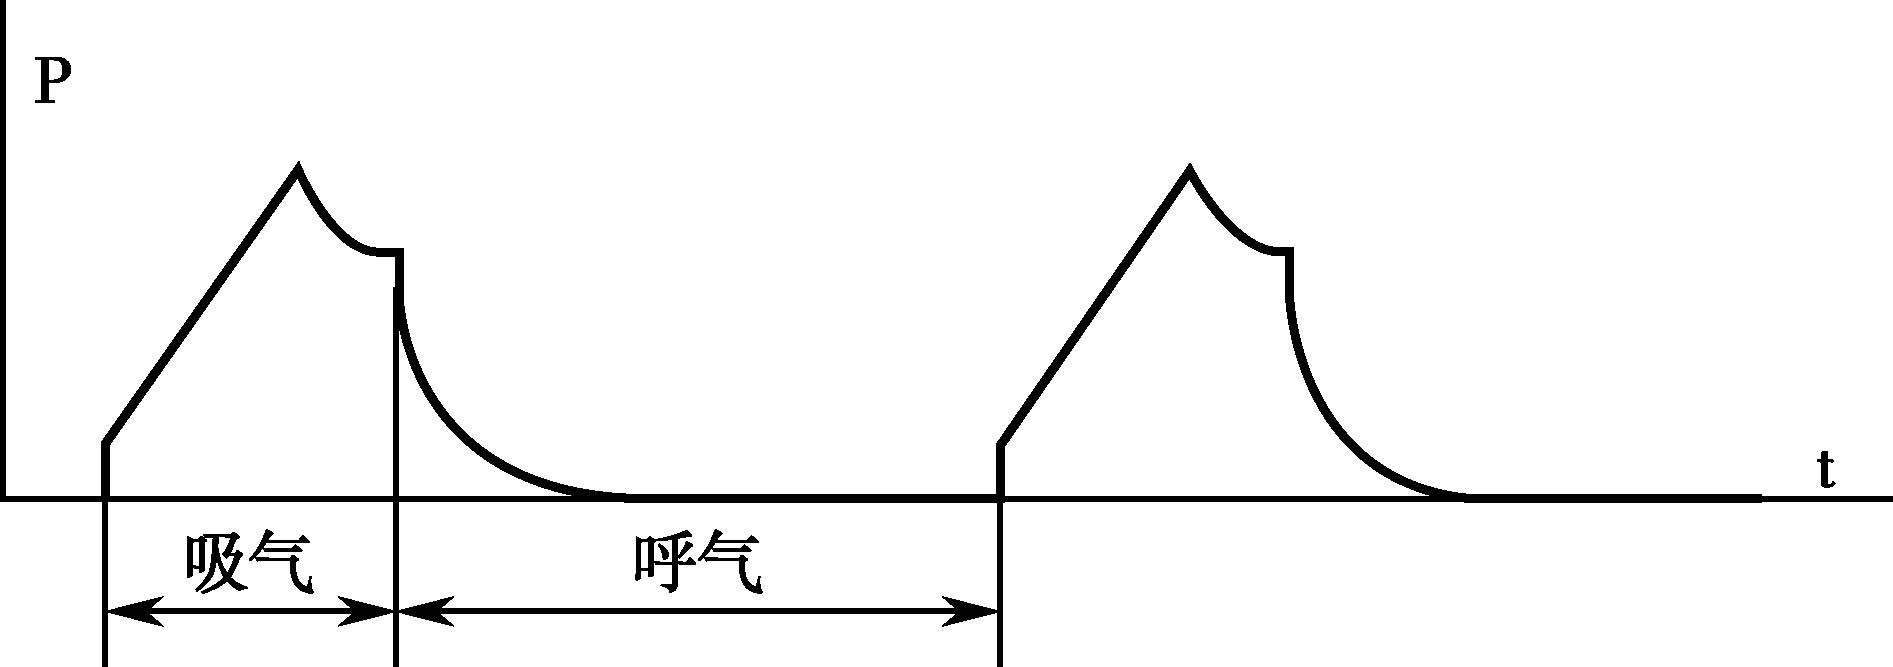
\includegraphics[width=3.11458in,height=1.09375in]{./images/Image00507.jpg}
 \captionsetup{justification=centering}
 \caption{间歇正压通气(IPPV)模式}
 \label{fig136-1}
  \end{figure} 

\hypertarget{text00368.htmlux5cux23CHP16-3-2-1-2}{}
(二) 持续正压气道通气(continuous positive airway pressure,CPAP)

CPAP是指在有自主呼吸条件下,整个呼吸周期内均由呼吸机产生一定水平的正压,辅助患者的呼吸动作,改善呼吸功能的通气模式,又可称为自主呼吸基础上的全周期正压通气(图\ref{fig136-2})。CPAP是一种独立的通气模式,虽然与呼气末正压(positive
end-expiratory
pressure,PEEP)相仿,也能增加FRC、防止气道闭合和肺泡萎陷,但因CPAP仅是一种自主呼吸的通气方式,呼吸机并不提供恒定的潮气容积与吸气流速,故在纠正由严重肺功能障碍所致的换气功能障碍时,远不如PEEP效果明显。由于CPAP对自主呼吸要求较高,许多有严重肺功能障碍的患者,不适合应用CPAP通气模式,这在相当程度上限制了其应用范围。CPAP通气模式的主要优点是吸气时恒定的持续正压气流>吸气气流,使吸气省力,呼吸作功减少;此外,呼吸机与患者连接的方式较为灵活,经人工气道或面罩均可。主要用于脱机前过渡或观察自主呼吸情况,如吸气压力、TV、MV等。CPAP对人体的影响与PEEP相同,如对循环干扰,回心血量减少、心排量下降、血压下降、心脏负荷增加和气压伤等。

\hypertarget{text00368.htmlux5cux23CHP16-3-2-1-3}{}
(三) 间歇指令通气(intermittent mandatory
ventilation,IMV)/同步间歇指令通气(synchronized intermittent mandatory
ventilation,SIMV)

IMV最初是为脱机设计和发明的通气模式。在IMV过程中,患者可以有自主呼吸,整个呼吸过程分指令与自主呼吸(图\ref{fig136-3})。用于撤离呼吸机时,通过逐渐降低指令呼吸频率,有助于锻炼患者应用自主呼吸维持呼吸功能。早先的IMV模式,不具备同步装置,以后为了让呼吸机提供的指令呼吸与患者的自主呼吸更好地协同,就发展成为有同步装置的SIMV,即便是呼吸机提供的指令呼吸,也可以通过呼吸机固有的同步装置,由患者吸气触发,并与自主呼吸配合。因此,目前呼吸机的模式基本均以SIMV替代了IMV。SIMV的优点是将IPPV与自主呼吸很好地结合和协调,不但能保证有效通气量,还能避免过度通气和通气不足,减少呼吸性碱中毒和酸中毒的发生;脱机过程中应用SIMV,可以逐渐减少呼吸机的辅助呼吸,充分发挥患者自身调节呼吸的能力,减少呼吸肌发生失用性萎缩的可能,也有助于逐渐撤离呼吸机,使从机械通气到自主呼吸的过渡更安全和可靠,避免脱机过程中的盲目性。多数情况下,当逐渐降低指令通气频率至5~8次/分,如果患者能维持较好的呼吸功能,且没有其他影响脱机的因素,基本就不存在脱机失败的顾虑了。随着呼吸机的临床应用,鉴于SIMV模式能较好地将指令与自主呼吸结合,既可以避免呼吸肌失用性萎缩,也不至于过于盲目依靠患者的自主呼吸,SIMV模式的应用范围在扩大,很多呼吸机上还配有定压型的SIMV,并与PSV组合,成为定压型的SIMV
+ PSV和定容型SIMV +
PSV。目前已经成为临床应用较普遍的一种通气模式,甚至替代了IPPV。值得注意的是,使用低频率(<
10次/分)SIMV的时间不宜过长,以免因为指令呼吸频率太少,自主呼吸又无PSV辅助,引起呼吸肌疲劳;通常在使用SIMV过程中,如果指令呼吸频率<
16次/分,就应常规加用(PSV)。此外,如果呼吸机的SIMV模式没有说明是定压或定容型,那就一定是定容型SIMV,特点与定容型模式相同。

\begin{figure}[!htbp]
 \centering
 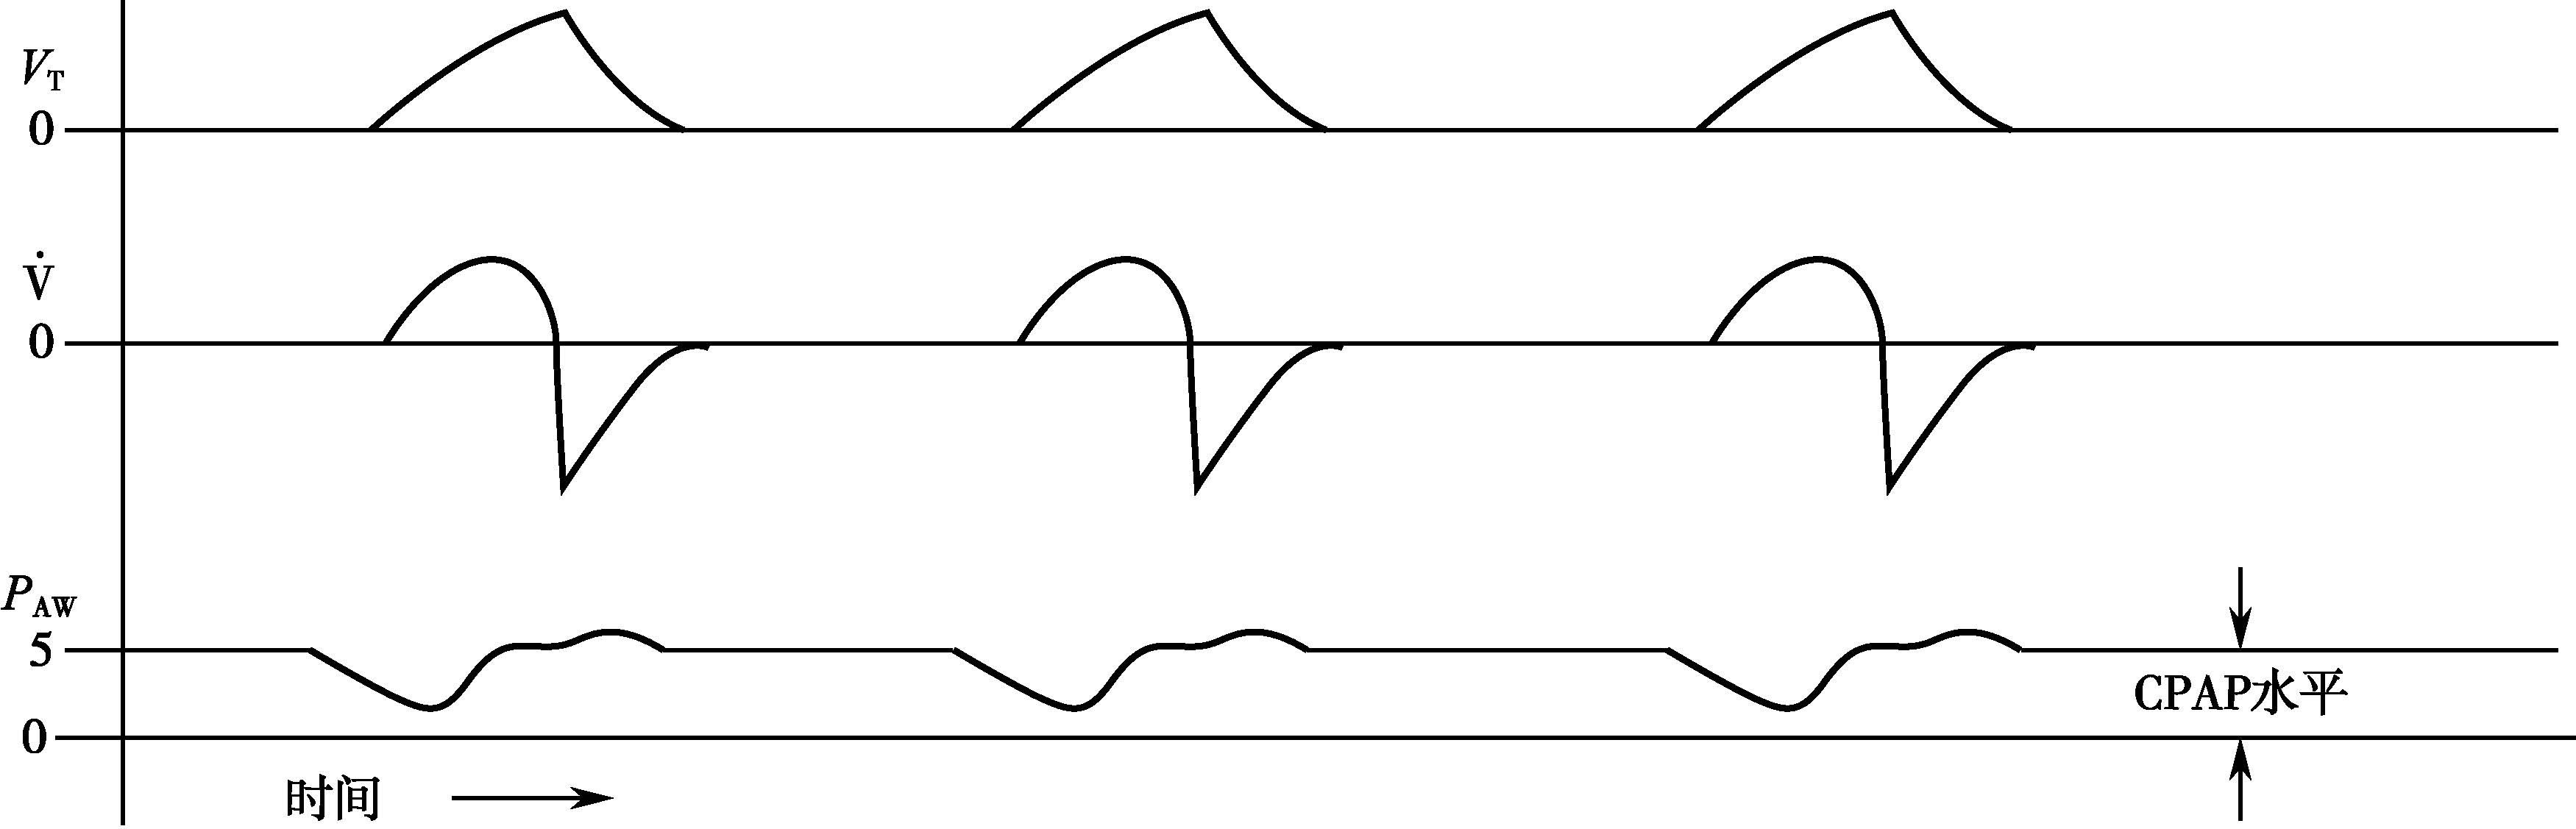
\includegraphics[width=5.83333in,height=1.875in]{./images/Image00508.jpg}
 \captionsetup{justification=centering}
 \caption{持续正压气道通气(CPAP)模式}
 \label{fig136-2}
  \end{figure} 

\begin{figure}[!htbp]
 \centering
 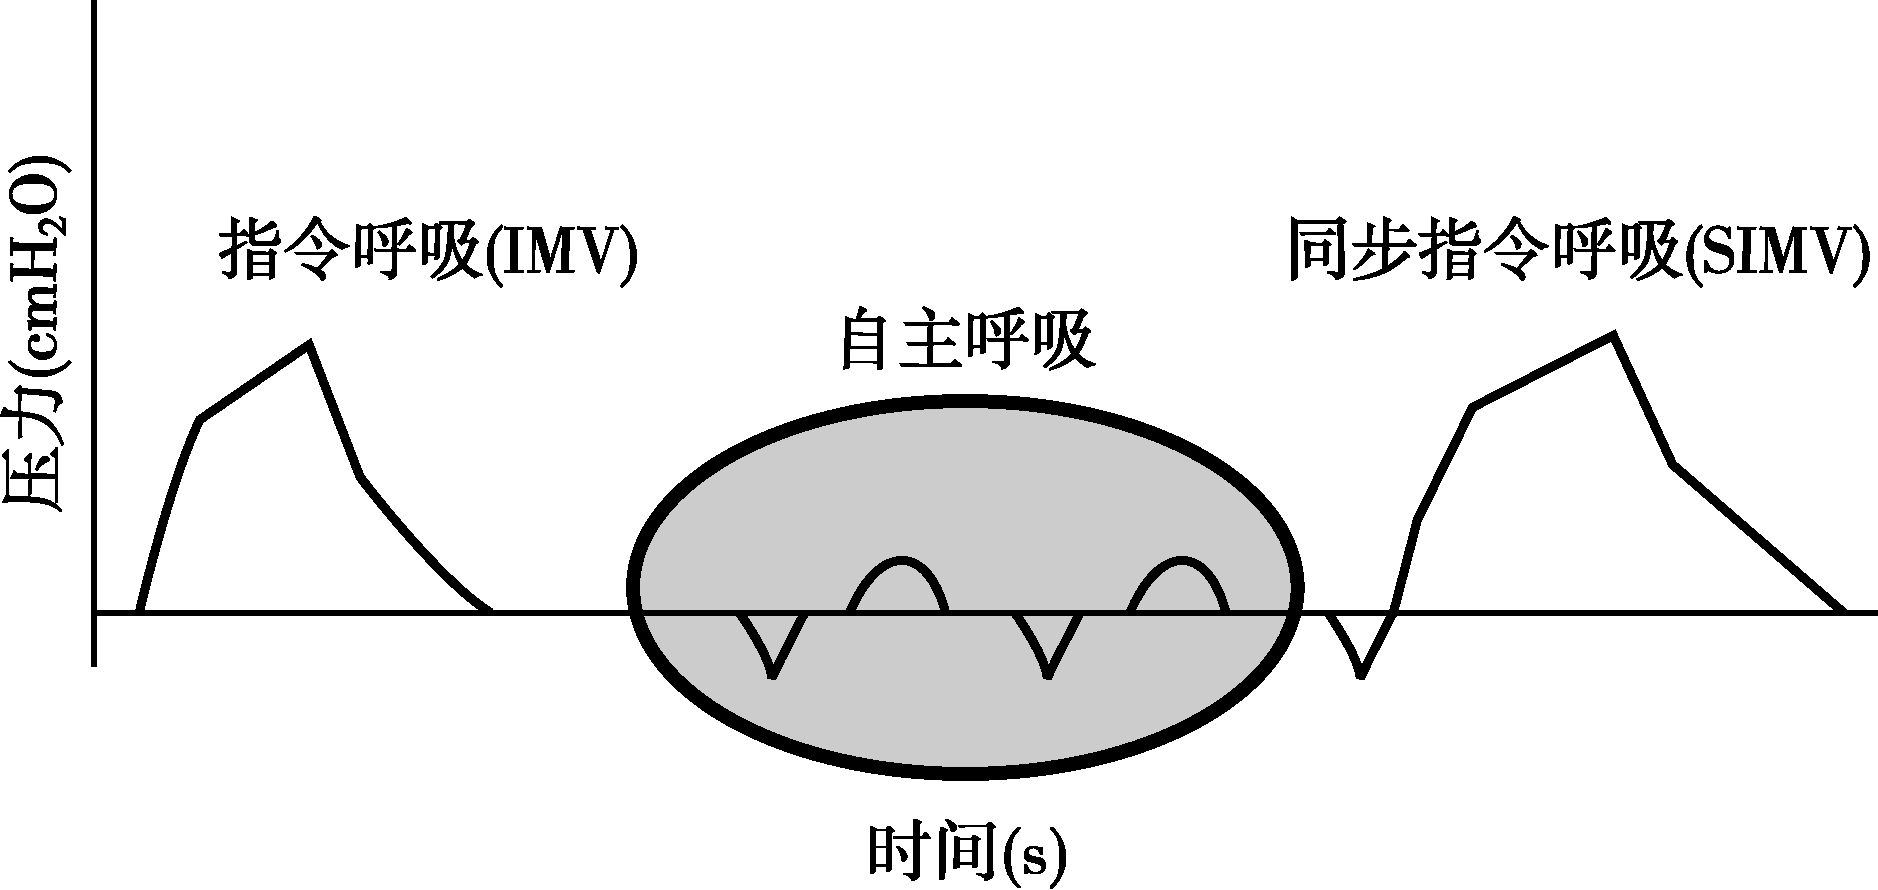
\includegraphics[width=3.125in,height=1.47917in]{./images/Image00509.jpg}
 \captionsetup{justification=centering}
 \caption{间歇指令通气/同步间歇指令通气(IMV/SIMV)模式}
 \label{fig136-3}
  \end{figure} 

\hypertarget{text00368.htmlux5cux23CHP16-3-2-1-4}{}
(四) 压力支持通气(pressure support ventilation,PSV)

PSV是一种辅助通气方式,即在自主呼吸的前提下,每次吸气都接受一定水平的压力支持,辅助患者的吸气能力,增加吸气幅度和吸入气量(图\ref{fig136-4})。PSV既可以作为一种独立的通气模式,辅助患者的呼吸动作,也可以作为一种通气功能与其他通气模式同时使用(图\ref{fig136-5})。应用时吸气压力或称支持压力需设定,并可以任意调节。吸气压力随吸气动作开始,随吸气流速减少到一定程度或患者呼气用力而结束。呼气用力时,即出现呼吸切换,其呼吸频率可以减慢,潮气量和吸气时间均可随意,而辅助通气的潮气量和吸气时间均是恒定的。PSV是类似带有同步装置的定压型辅助呼吸,但吸气相压力恒定,吸气到呼气切换方式不尽相同。PSV与SIMV通气模式的不同之处,是患者的每次吸气,均可得到压力的支持,但支持的水平可随需要不同而可设定。临床应用适用于自主呼吸能力不足,但神经调节无明显异常的患者。

\hypertarget{text00368.htmlux5cux23CHP16-3-2-1-5}{}
(五) 双水平正压通气(Bi-level positive airway pressure,BiPAP)

BiPAP是80年代中后期产生的通气模式,起初用于治疗ARDS,其实质是一种定压型的通气模式。BiPAP模式下,通过调节两个压力(P\textsubscript{1}
与P\textsubscript{2} )和两个时间(T\textsubscript{1}
与T\textsubscript{2}
)的调节,可以调节出不同的定压型通气模式,CMV或AMV(图\ref{fig136-6})。BiPAP模式的两个压力设置可以完全不同,分高(Phigh)和低(Plow)压;依据Phigh和Plow,两个时间也可以不同,分别为高压(Thigh)和低压(Tlow)时间。临床应用时,Phigh和Plow、Thigh和Tlow可以被任意设置与组合,并相当于不同的通气模式。如果以CMV为例,依据设置的压力不同,所形成的压力变化图形,分别相当于CMV-BIPAP、IMV-BIPAP、传统(genuine)-BIPAP、CPAP等。但无论怎样设置,所有的模式均可能是PCV模式。PCV与BIPAP主要的不同点是,PCV模式下,患者在吸气相,不能任意地进行自主呼吸;而在BIPAP模式下,各个周期均允许患者存在或出现任意的自主呼吸(图\ref{fig136-7}),故具备同步性能好、舒适、镇静药使用减少等。因此,BIPAP是将PCV与自主呼吸结合最好的通气模式(图\ref{fig136-8})。BiPAP模式临床应用较广,但鉴于其是定压型通气模式,不适用于气道阻力增加、需要吸气压力过高的患者,如对支气管哮喘的患者,常可能出现潮气量不保证。保护性肺通气策略(lung
protective ventilatory strategy,LVPS)与肺开放(open
lung)/复张(recruitment
maneuver,RA)提出后,应用BiPAP模式实施肺开放/复张策略,取得较好的疗效。

\begin{figure}[!htbp]
 \centering
 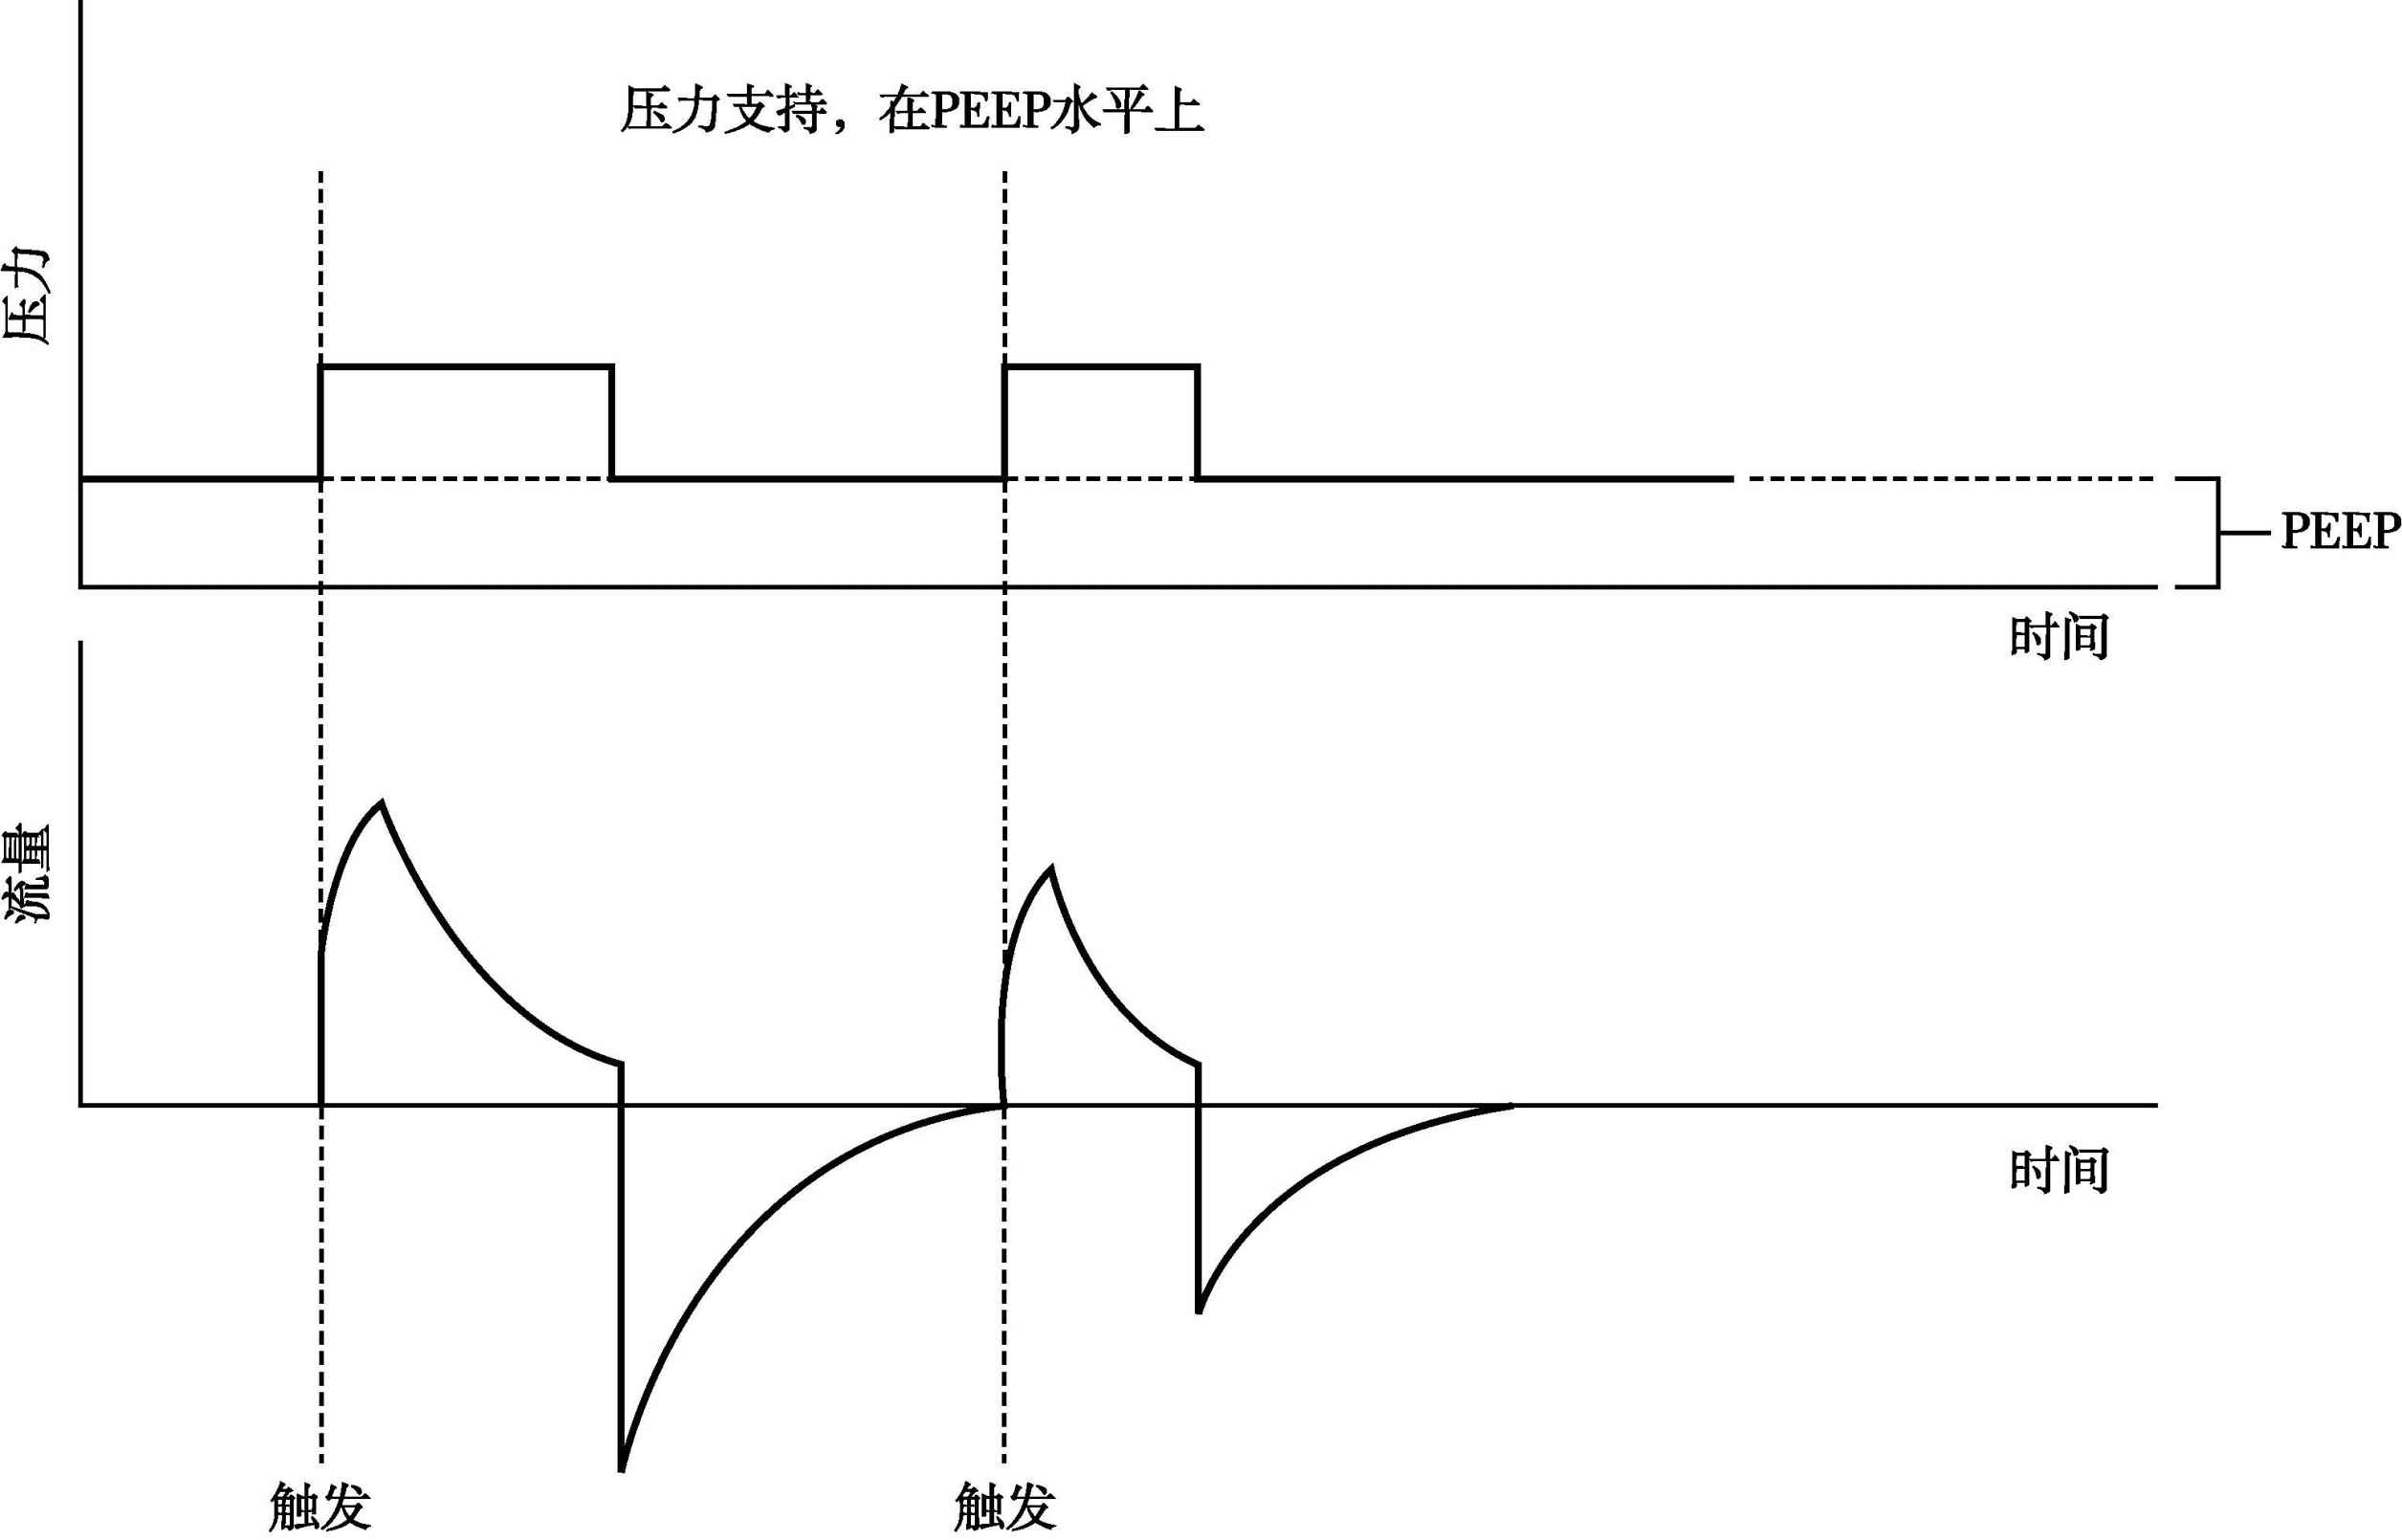
\includegraphics[width=5.16667in,height=3.3125in]{./images/Image00510.jpg}
 \captionsetup{justification=centering}
 \caption{压力支持通气(PSV)模式}
 \label{fig136-4}
  \end{figure} 

\begin{figure}[!htbp]
 \centering
 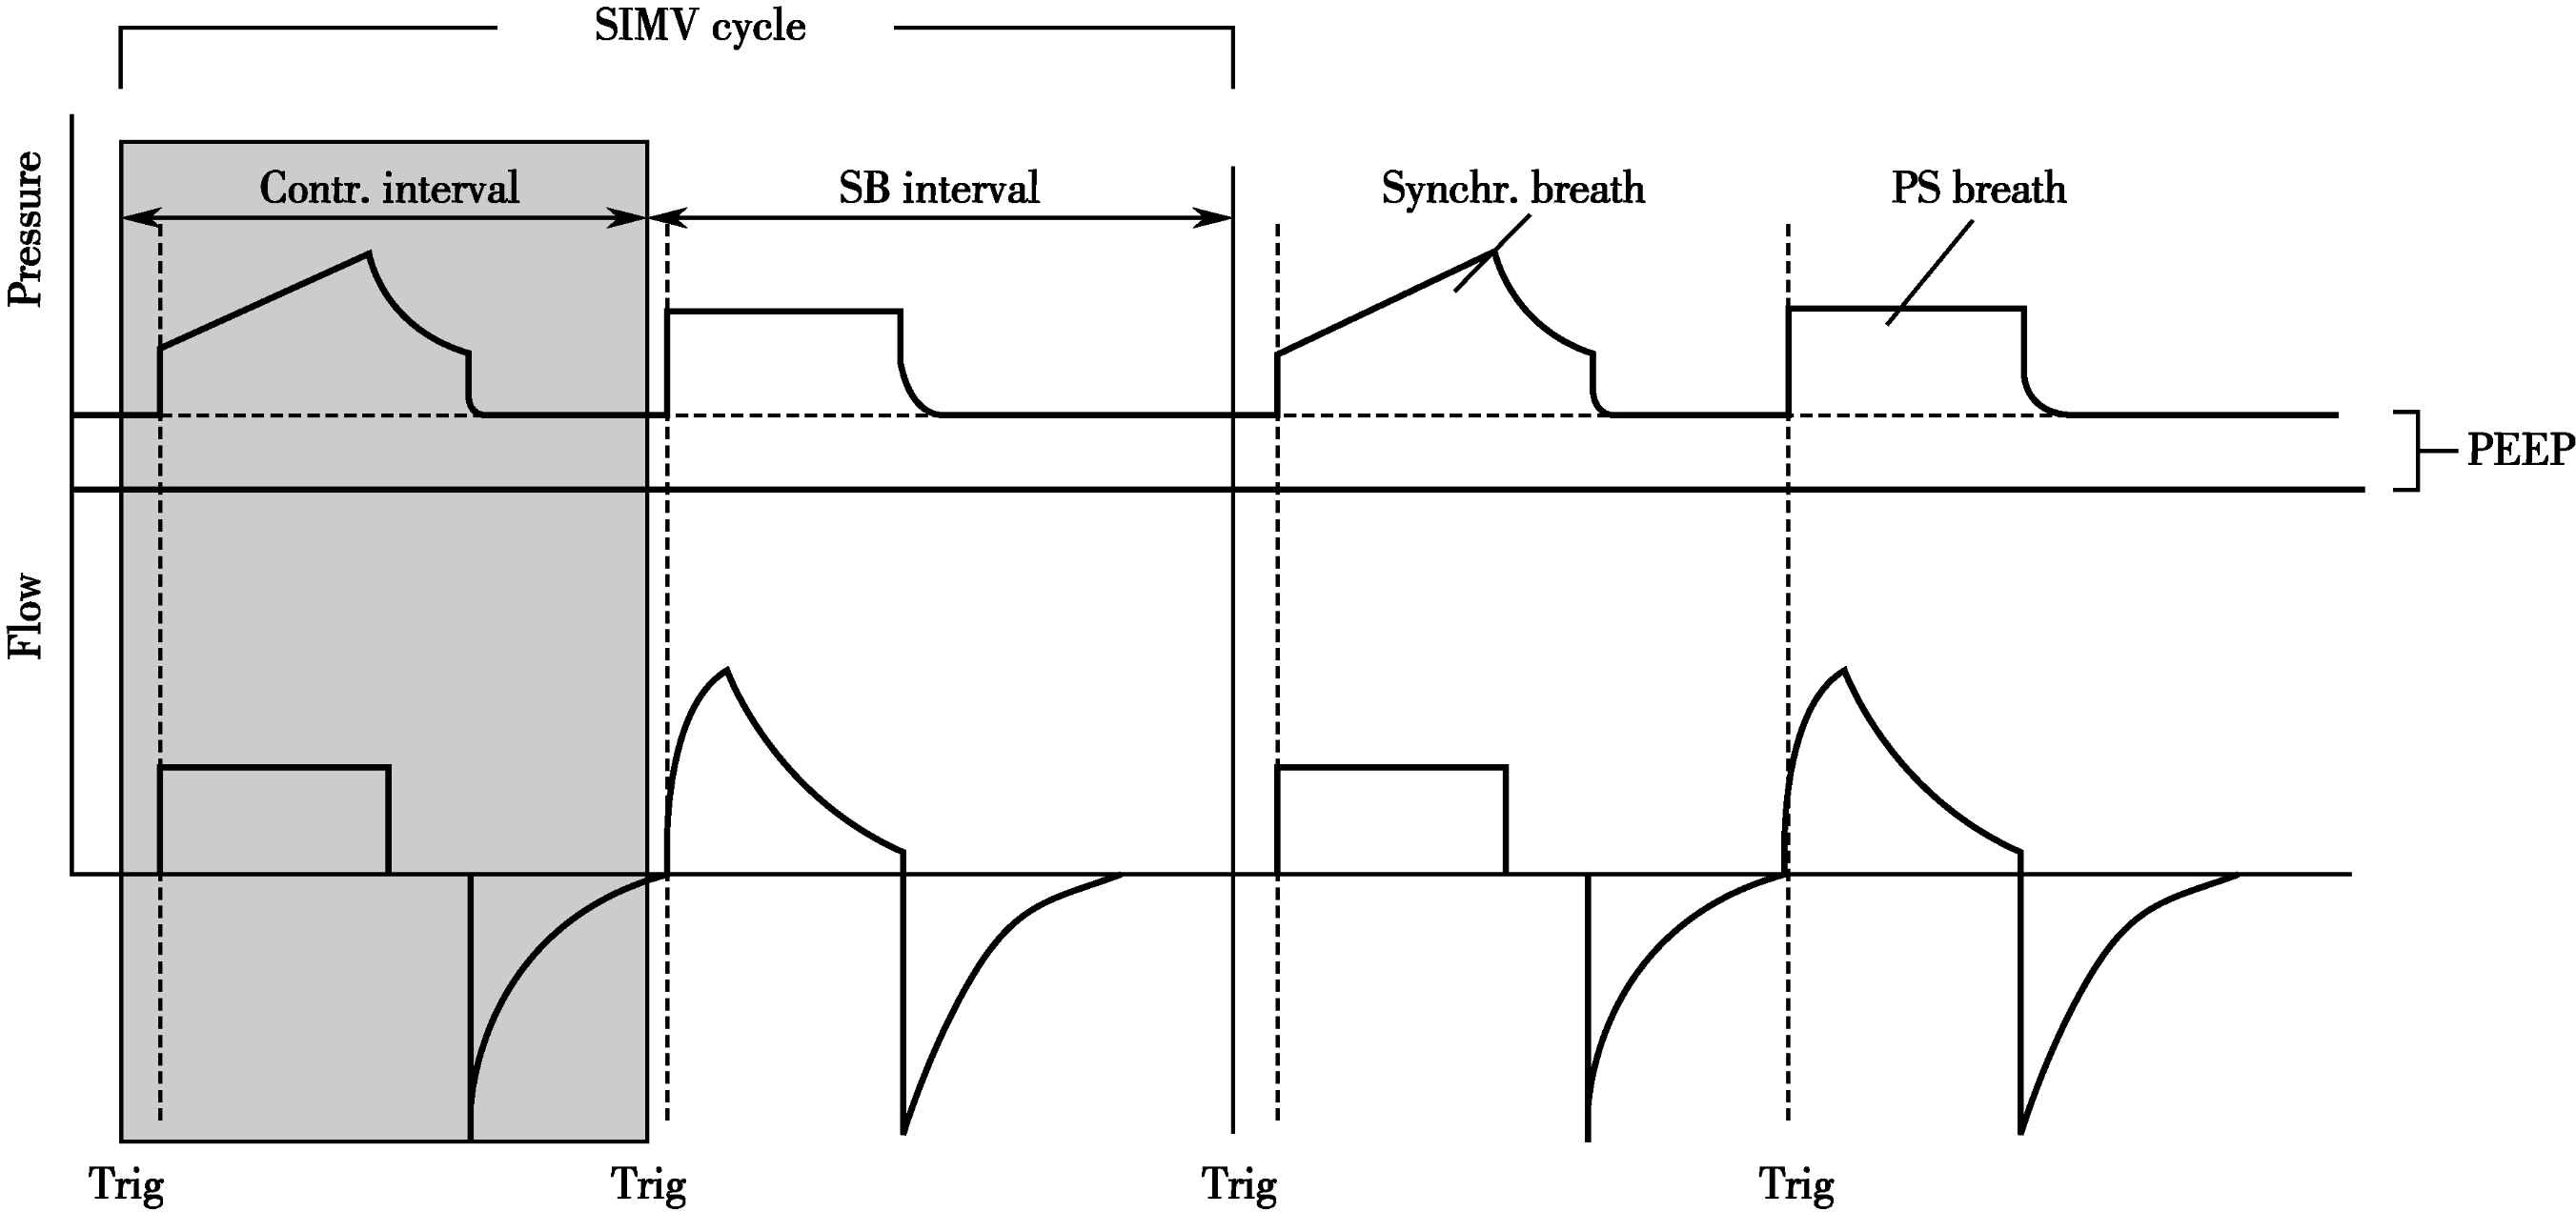
\includegraphics[width=6.15625in,height=2.89583in]{./images/Image00511.jpg}
 \captionsetup{justification=centering}
 \caption{间歇指令通气/同步间歇指令通气+压力支持通气(IMV/SIMV +}
 \label{fig136-5}
  \end{figure} 
PSV)模式

\begin{figure}[!htbp]
 \centering
 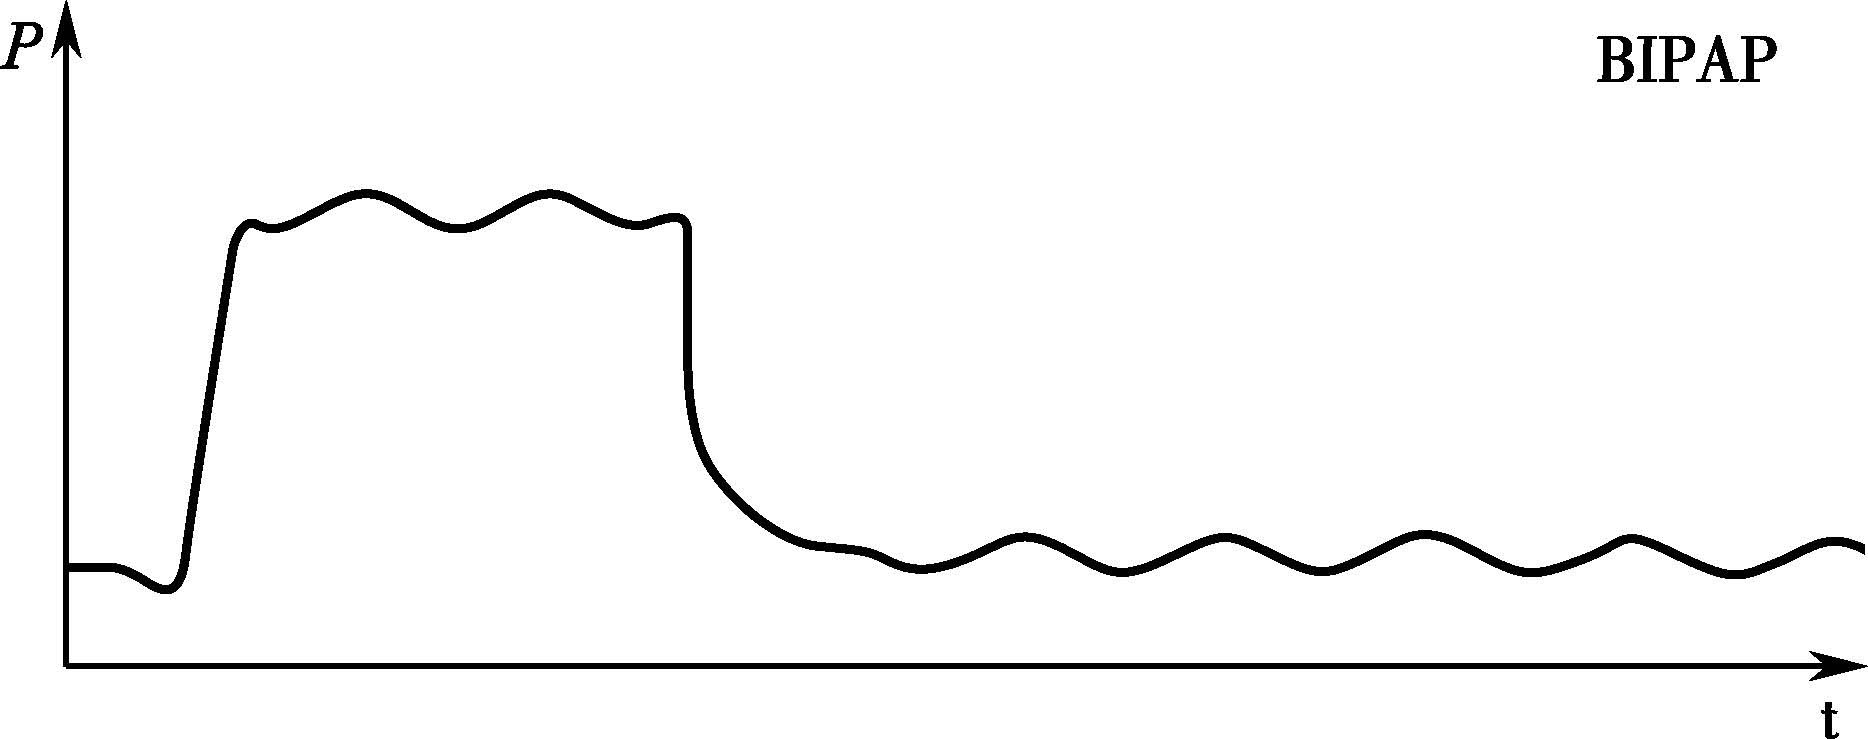
\includegraphics[width=3.10417in,height=1.22917in]{./images/Image00512.jpg}
 \captionsetup{justification=centering}
 \caption{两个压力水平下的 CMV或AMV}
 \label{fig136-6}
  \end{figure} 

\hypertarget{text00368.htmlux5cux23CHP16-3-2-1-6}{}
(六) 压力/容量双控模式

随着呼吸机生产工艺的迅速发展与改进,多功能型呼吸机已经逐渐替代了以往单纯PC或VC型呼吸机,但呼吸机模式还存在PCV或VCV之分。由于PCV或VCV模式各有利弊,压力/容量双控模式的发明与产生,正是为了克服它们的弊,集中它们的利为一体。因此,双控模式的出现,使呼吸机的使用达到了更加高度智能化的水平。

\subparagraph{压力调节容量控制(pressure regulated volume control,PRVC)}

PRVC模式的优点是能在确保预置VT等参数的基础上,通过自动连续监测胸廓/肺顺应性和P-V,反馈调节下一次通气的吸气压力,以将气道压力控制在最低水平,不但能确保恒定的VT,还能减少气压伤。PRVC与
VSV相比,有相同处,也有不同处。相同处是两种通气模式均受压力和容量双重调节;不同处是PRVC既可以用于控制性呼吸,也可以用于辅助性呼吸。PRVC模式下,患者的呼吸可以不由患者的自主呼吸触发,而是机器按操作者设置的参数工作,患者的呼吸频率、I∶E、压力及容量(VT、MV)等,均可以预先设置。PRVC模式最适合用于有肺力学改变的患者,尤其是气道阻力增加,顺应性严重下降的患者,代表性的疾病是严重支气管哮喘和ARDS。

\begin{figure}[!htbp]
 \centering
 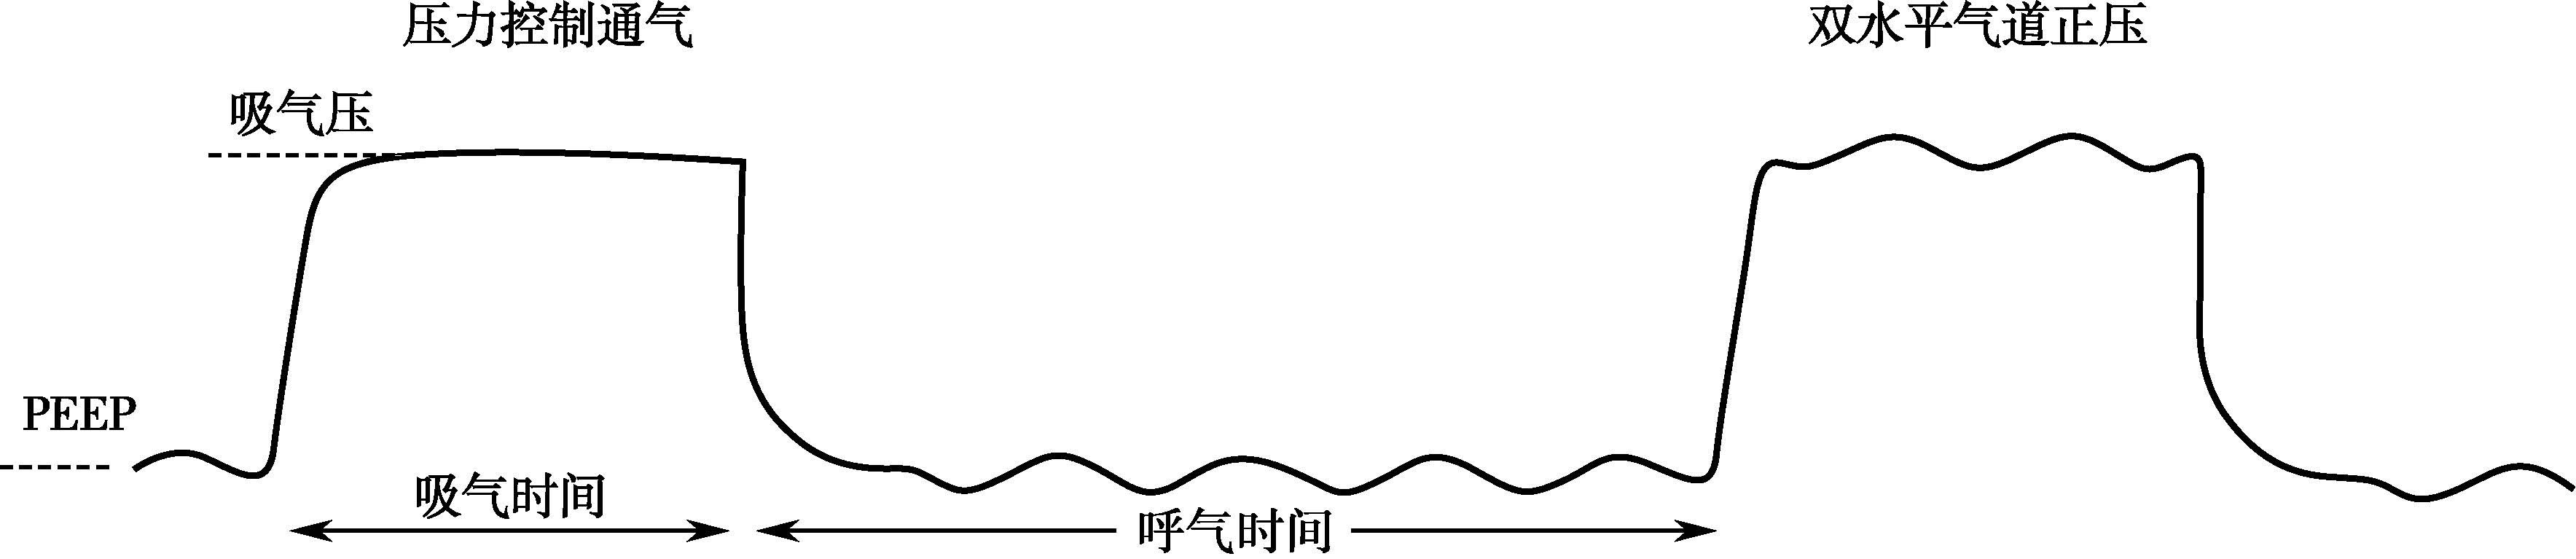
\includegraphics[width=5.88542in,height=1.27083in]{./images/Image00513.jpg}
 \captionsetup{justification=centering}
 \caption{BIPAP各个周期均允许患者存在或出现任意的自主呼吸}
 \label{fig136-7}
  \end{figure} 

\begin{figure}[!htbp]
 \centering
 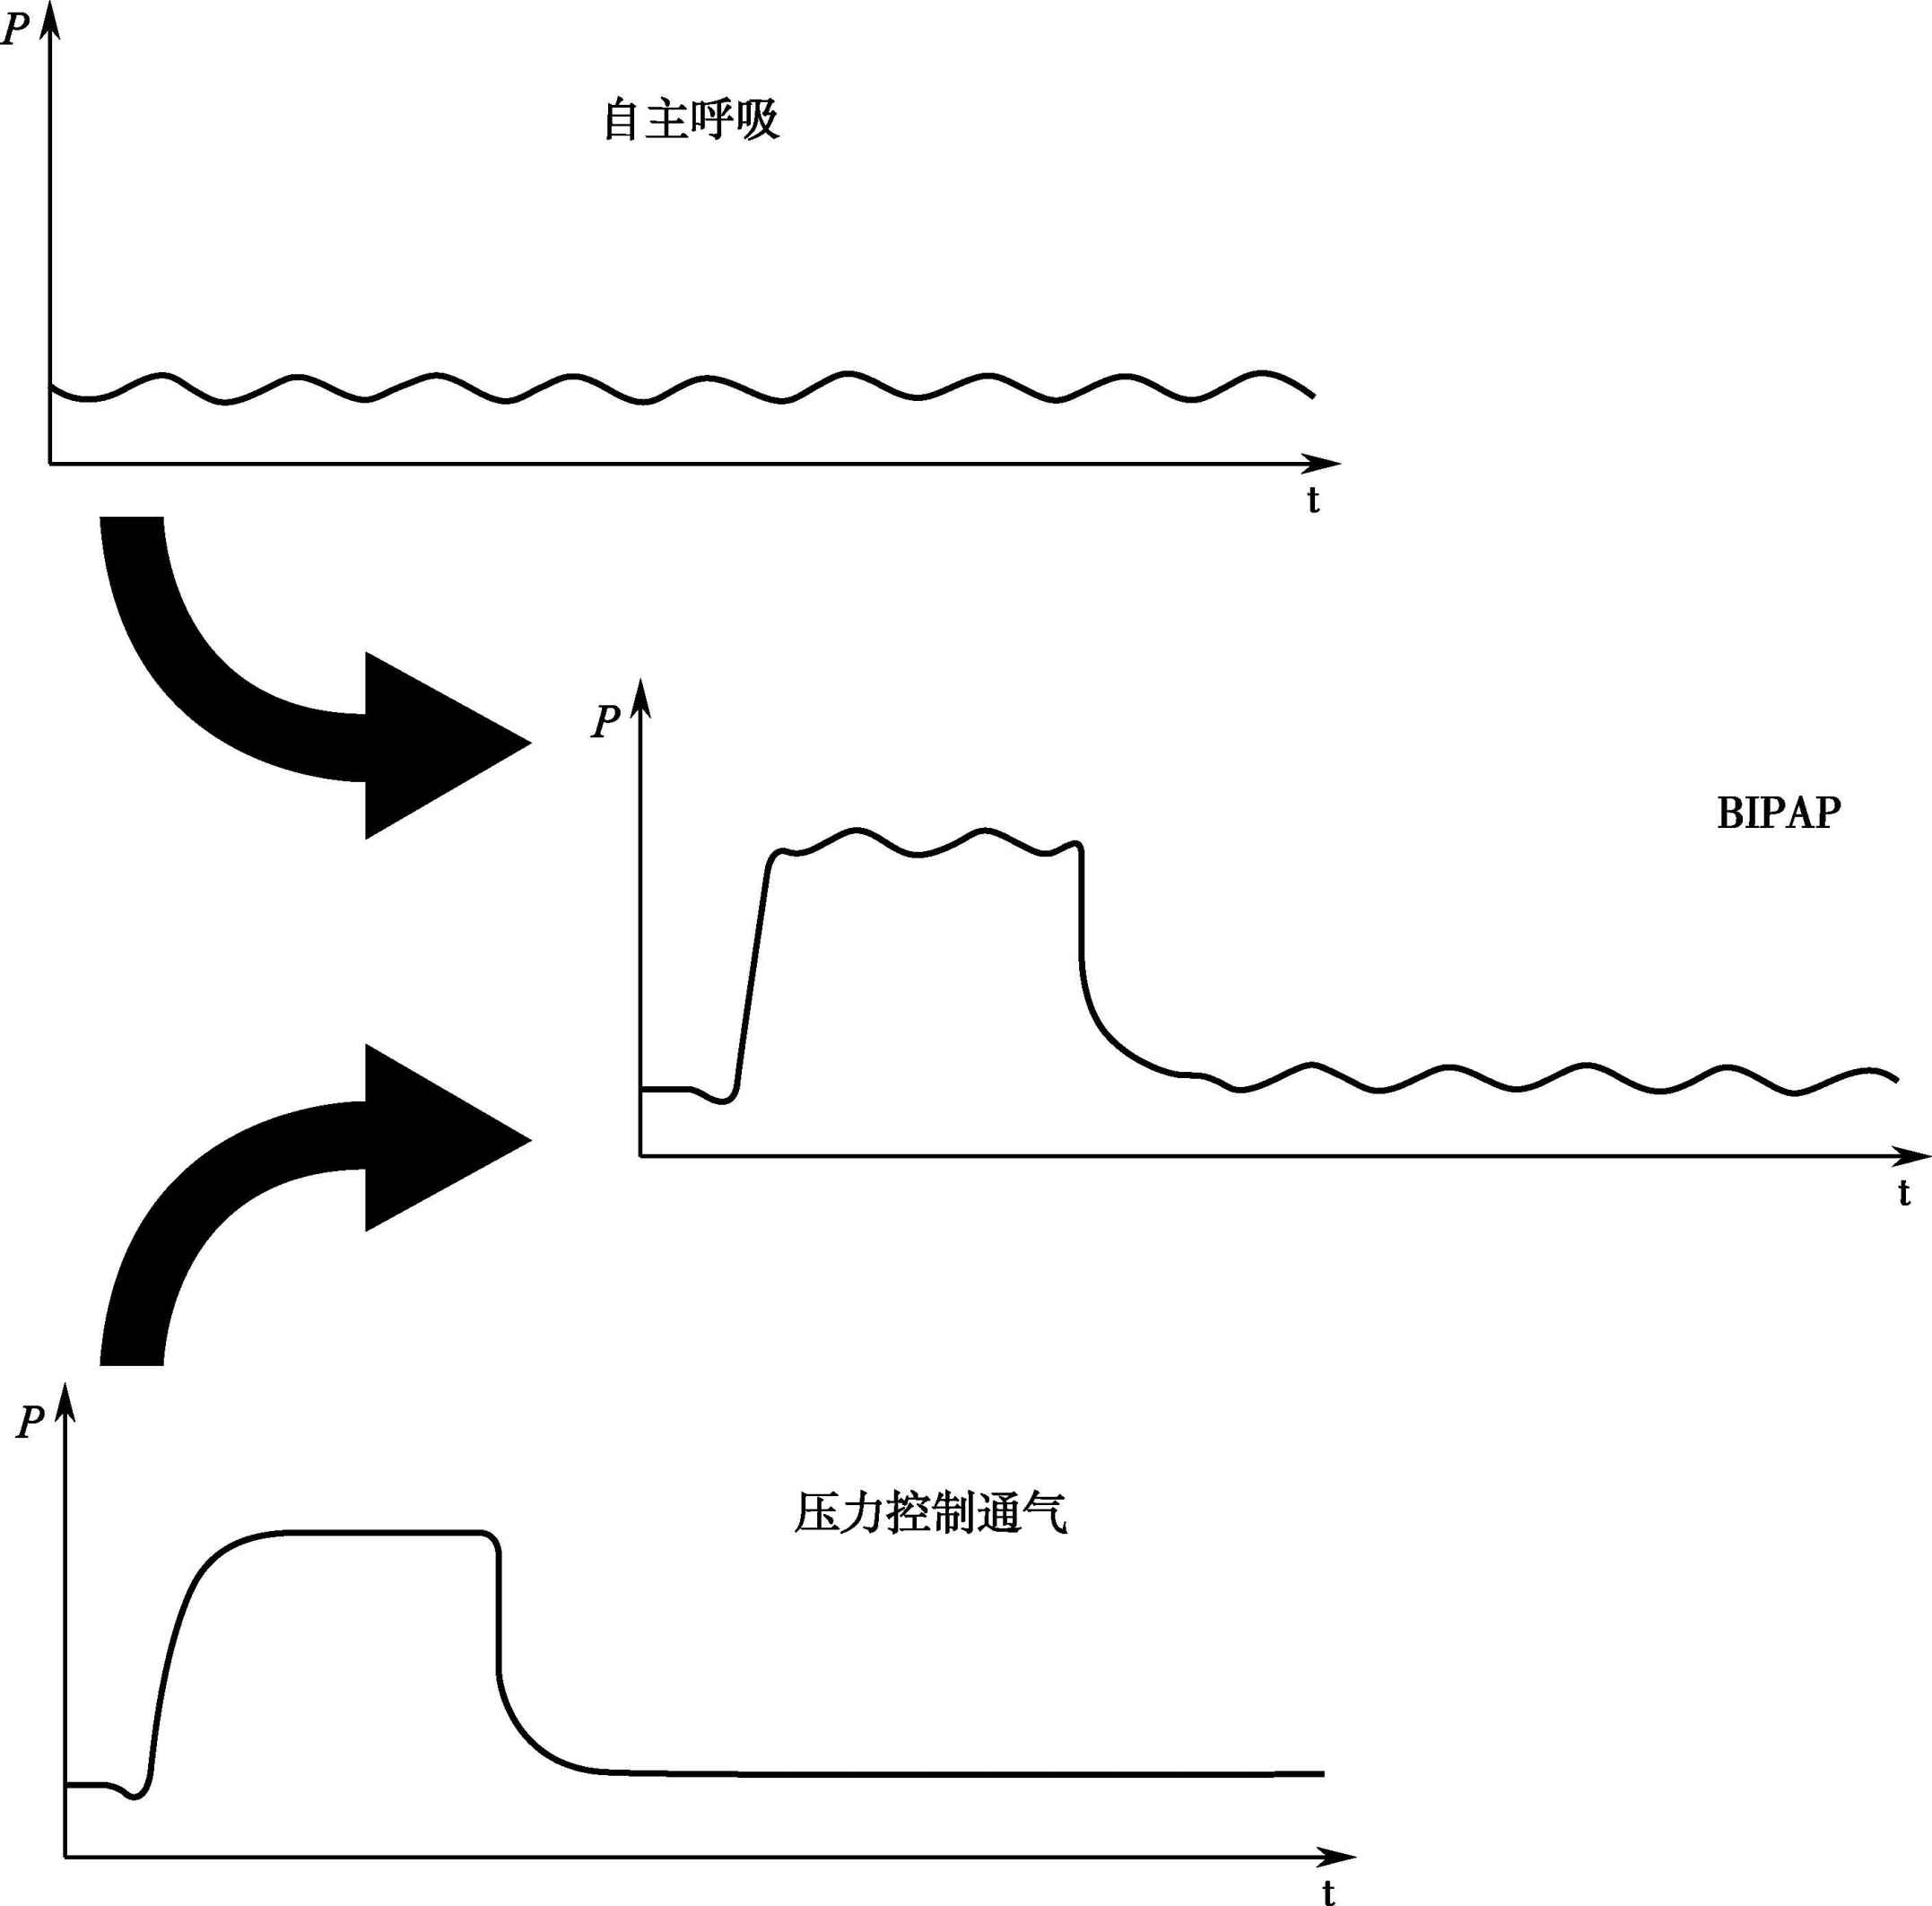
\includegraphics[width=4.6875in,height=4.625in]{./images/Image00514.jpg}
 \captionsetup{justification=centering}
 \caption{BIPAP将PCV与自主呼吸很好结合}
 \label{fig136-8}
  \end{figure} 

\subparagraph{容量保证压力支持(volume assured pressure support,VAPS)}

VAPS模式与PRVC模式相比,目标一致,但调节机制不同。VAPS模式又被称为压力扩增(pressure
augmentation,PA)模式,它是将容量辅助通气(VAV)与PSV很好地结合,呼吸机以容量切换为基础,以PSV模式或功能作为容量保证的主要途径,即呼吸机将预设的VT输送给患者后即转为呼气,能避免PSV中VT不保证的缺点。当患者无自主呼吸、PSV模式或功能无法实施时,即转换为VCV模式。因此,VAPS模式通常只需要一次呼吸周期就能达到预定的容量目标,而PRVC模式则可能需要三次呼吸周期才能达到预定的容量目标,这是两者最主要的区别。

\hypertarget{text00368.htmlux5cux23CHP16-3-2-1-7}{}
(七) 指令分钟通气(mandatory minute ventilation,MMV)

MMV模式的工作原理是通过微电脑持续监控患者的分钟通气量,操作者依据患者的年龄、性别、身高、体重、体表面积或动脉血气分析等,预设好一定水平的分钟通气量,如单位时间内自主呼吸的通气量已达到或超过预设的分钟通气量水平,呼吸机则不作指令通气,而只提供一个持续的正压气流,供自主呼吸时用;如单位时间内自主呼吸的通气量低于预设的分钟通气量水平,无需操作者调节呼吸机,呼吸机就会自动通过增加指令通气方式,增加分钟通气量,使其达到预设的分钟通气量水平。采用MMV通气模式时,无论患者的自主呼吸如何,呼吸机均能保证患者得到足够的分钟通气量,即预设的分钟通气量。MMV模式类似于IMV/SIMV,能减少呼吸性碱中毒的发生、减少正压通气对循环和肺组织的影响,有助于充分发挥患者的自主呼吸能力,锻炼和维持患者呼吸肌的功能。

\hypertarget{text00368.htmlux5cux23CHP16-3-2-1-8}{}
(八) 容量支持通气(volume support ventilation,VSV)

VSV模式的实际临床意义与MMV通气方式类似,不同点是具体的调节机制。应用VSV通气模式时,呼吸机的每一次供气均由自主呼吸触发,当实际TV或MV低于或高于设置的TV或MV时,呼吸机可通过自动反馈信息,使TV和MV增加或降低,以达到实际通气量不变或恒定的目的。采用VSV时,呼吸频率和吸/呼(I∶E)均由患者自己调节。VSV通气模式下,如果每一次呼吸均由患者自主呼吸触发,患者也可以不要任何支持进行呼吸,并能达到预设的TV和MV水平,呼吸机允许患者进行真正的自主呼吸,通气本身将只是起到监测患者实际TV或MV的作用。与PSV相似,自主呼吸停止时,呼吸机不被触发,呼吸机不可能供气。为防止意外,该通气模式下通常设有呼吸暂停时间阈值(apnea
limit),当自主呼吸停止时,呼吸机可自动转换为另一种呼吸模式,以维持相对正常的呼吸。VSV与PSV通气模式比较,优点是能自动根据患者肺力学特点,如气道阻力和肺、胸的顺应性,调整能达预设TV和MV所需的最低吸气压力;能以最可能低的压力或压力支持,达到最合适的通气量,即可将呼吸机造成气压伤的可能性,降低到最低限度;能将自主呼吸的能力和机械通气机辅助呼吸的作用很好地结合和协调,既能充分发挥自主呼吸的能力,又能保障足够和安全的通气。这些均是PSV通气模式所不可及的。应用VSV通气模式时,气道压上限值的设置不能过低,否则有可能因机器所能调节的最高吸气压力均低于设置压力限制水平下5cmH\textsubscript{2}
O,而导致实际TV低于预设的TV,造成通气不足。VSV通气模式时,每次呼吸均有赖于患者自主呼吸的触发,倘若呼吸机与自主呼吸协调不好,呼吸机监测误差的增加,每次数据不一致而引起吸气压力水平多变,可能使患者感到不适。故应用VSV通气模式时,对患者的自主呼吸要求较高。如遇呼吸机与自主呼吸协调不好时,应及时采取措施协调呼吸机,否则应立即改变通气模式。

\hypertarget{text00368.htmlux5cux23CHP16-3-2-1-9}{}
(九) 压力释放通气(airway pressure release ventilation,APRV)

APRV的实质是一种定压型通气模式,即呼吸机按照设置能使吸气压力维持在一定水平,以达到满意的潮气量,并相当于在CPAP下的辅助通气模式。所不同的是,在呼气的回路,装有电动或气动的压力释放阀,能按要求使CPAP降低至零或某个预先设置的水平,一定时间后再重新回到CPAP水平,并重复上述的辅助呼吸程序。APRV模式与所有定压型通气模式一样,由于潮气量不保证,不适合用于有气道阻力增加的患者。优点是能控制和降低气道峰压在一定水平,避免胸内压过高引起的血流动力学改变;能通过压力释放至一定水平(高于零),即相当于

PEEP作用,改善气体分布与{}
失调,纠正缺氧;允许患者在任何压力和时间相存在自主呼吸,如果与呼吸机协调得好,患者会感到十分舒适。APRV可作为一种通气模式,独立存在于某种类型的呼吸机上,也可以通过BiPAP模式实施。BiPAP模式下,当设置Phigh或P\textsubscript{1}
> Plow和P\textsubscript{2} ,且Thigh或T\textsubscript{1} >
Tlow和T\textsubscript{2}
时,即相当于APRV-BIPAP,其实质是PCV模式下的反比通气(inverse ratio
ventilation,IRV),即PC-IRV-BIPAP。

\hypertarget{text00368.htmlux5cux23CHP16-3-2-1-10}{}
(十) 成比例辅助通气(proportional assisted
ventilation,PAV)或成比例压力支持(proportional pressure support,PPS)

PAV与PPS模式临床应用也不普遍,实用价值亟待探讨。通气原理是呼吸机通过对吸气压力或流速的成比例辅助和支持,维持呼吸功能,减少呼吸作功。呼吸机对自主呼吸辅助和支持的比例是可以设置的,优点是如果呼吸功能得到满足,呼吸机与患者的协调好,患者感觉舒适,避免由于参数设置不佳造成的过度通气或通气不足,减少镇静剂使用,避免气道压力过高。与定压型呼吸模式相同,应用PAV/PPS模式时,要充分了解患者气道阻力和胸肺顺应性的改变,否则通气量会无法保障;此外,导管漏气也可以影响PAV/PPS模式的功能。PPS与PSV的区别在于,PSV压力支持水平恒定,只要患者触发,呼吸机就可能给予支持;PPS随吸气力的变化,给予压力支持,对患者的自主呼吸作最合适的调节。这些模式临床应用并不普遍,实用价值亟待探讨。

\subsubsection{呼吸机功能}

呼吸机拥有的功能很多,尤其是近年来的发展,各种不同类型功能相继出现。本章仅就常用的呼吸机功能简介如下。

\hypertarget{text00368.htmlux5cux23CHP16-3-2-2-1}{}
(一) 呼气末正压通气(positive end-expiratory pressure,PEEP)

正常在IPPV通气模式下,呼气时压力降为零,而PEEP是指呼吸机所具备的,能在呼气末仍保持一定水平正压的功能(图\ref{fig136-9})。

\begin{figure}[!htbp]
 \centering
 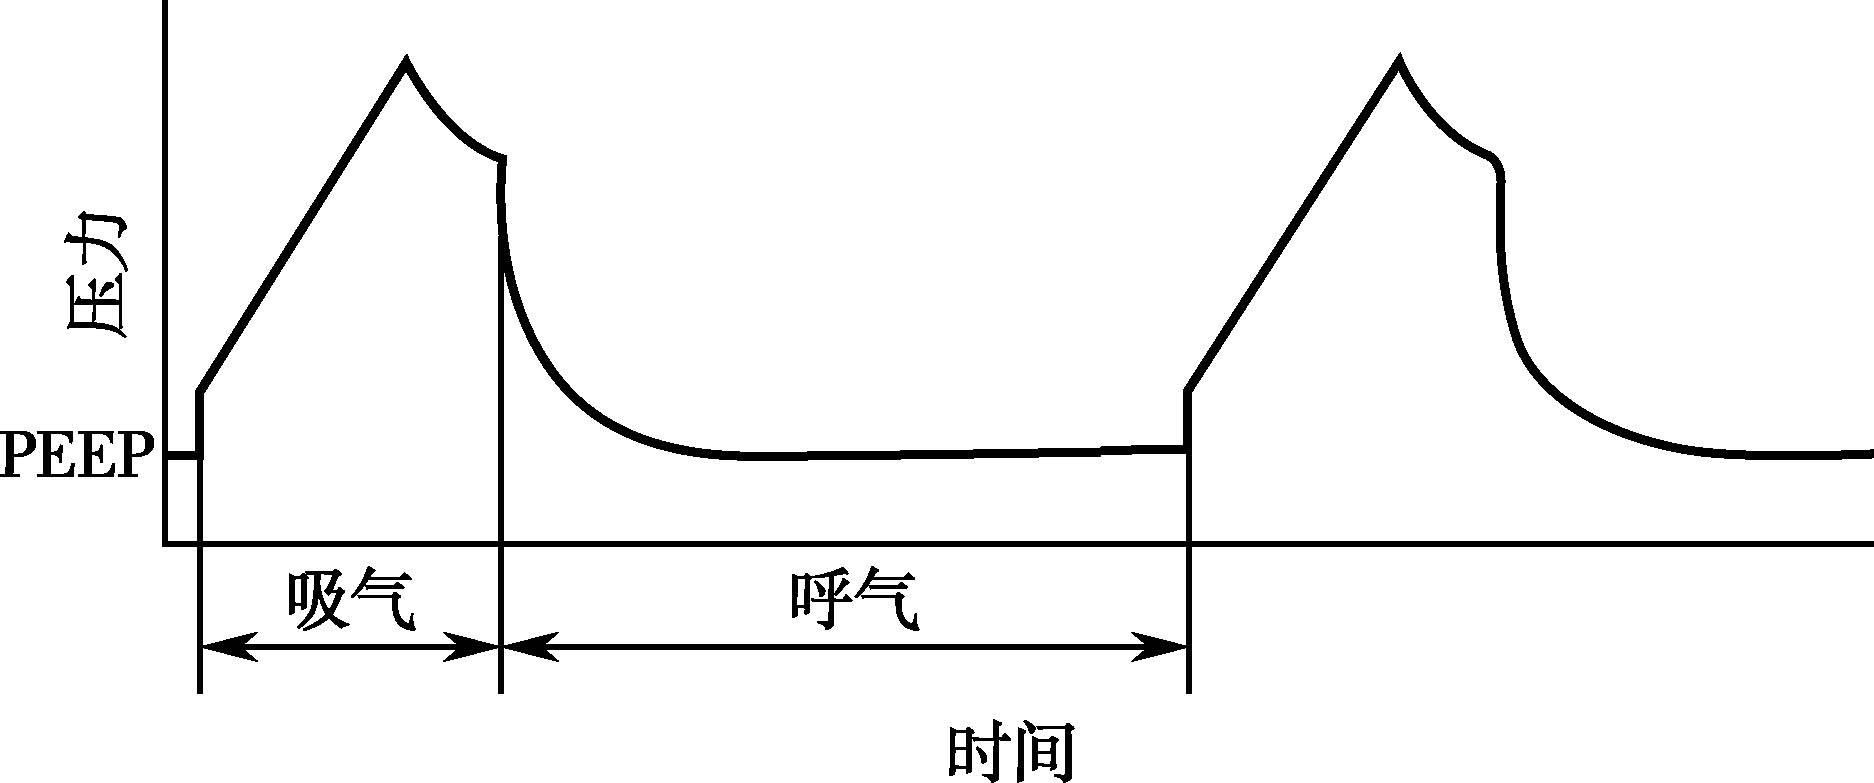
\includegraphics[width=3.11458in,height=1.30208in]{./images/Image00516.jpg}
 \captionsetup{justification=centering}
 \caption{呼气末正压通气(PEEP)}
 \label{fig136-9}
  \end{figure} 

\subparagraph{临床应用}

主要适用于由{}
增加所致的低氧血症,如以ARDS为代表的临床疾病。PEEP纠正ARDS低氧血症的作用机制是避免和防止小气道的闭合,减少肺泡萎陷,降低{}
,纠正由{}
增加所致的低氧血症;增加FRC,有利于肺泡-毛细血管两侧气体的充分交换(O\textsubscript{2}
与CO\textsubscript{2} );肺泡压升高,在FiO\textsubscript{2}
不变的前提下,能使D(A-a)O\textsubscript{2}
升高,有利于氧向肺毛细血管内弥散;PEEP使肺泡始终处于膨胀状态,能增加肺泡的弥散面积,也有助于氧的弥散;肺泡充气的改善,能使肺顺应性增加,在改善肺的通气、弥散{}
失调的同时,还可减少呼吸作功。

\subparagraph{最佳PEEP选择}

是能使萎陷的肺泡膨胀至最好状态、{} 降低至最低水平、PaO\textsubscript{2}
被提高至基本满意水平,而对血流动力学影响和肺组织气压伤降低至最低程度的PEEP水平。随疾病和病情严重程度不同,最佳PEEP水平不同;即使是同一个患者,在疾病发生和发展的不同阶段,所需要的最佳PEEP也可能不同。最佳PEEP选择一直是受关注的热点,至今仍无十分简便易行的方法。有主张通过观察压力-容量曲线(F-V)环下拐点(down
inflection
point,DIP)的方法,寻找最佳PEEP水平;有主张在CT扫描下,依据萎陷肺泡复张的状况,选择最佳PEEP;临床应用最多的,还是选择循环能承受、FiO\textsubscript{2}
≤60\%、PaO\textsubscript{2}
≥60mmHg时的最低PEEP水平。应用过程中,还需要根据氧合改善与恶化具体情况,随时调节PEEP水平。

\subparagraph{内源(内生)性PEEP(PEEPi)或自发性PEEP(auto-PEEP)}

指因呼气时间短或呼吸阻力过高,致肺泡内气体滞留,使肺泡内压在整个呼吸周期均保持正压,相当于PEEP的作用,称PEEPi或auto-PEEP。多由疾病造成,如当某种疾病使呼吸道阻力增加时,呼气所需的时间延长,在呼吸频率增加的情况下,由于呼气时间的缩短和同等时间内气道阻力增加所致的呼出气的减少,吸入的气体明显多于呼出的气体;随肺泡内气体逐渐增多,肺泡内压逐渐增加,PEEPi即由此产生。克服PEEPi的常用方法是应用相同水平的PEEP。

\hypertarget{text00368.htmlux5cux23CHP16-3-2-2-2}{}
(二) 呼气延长或延迟(expiratory retard)和呼气末屏气(end-expiratory
hold)

根据等压点(equal pressure
point,EPP)学说,呼气延长或延迟可减少气道(小支气管)的动态压缩,有助于气体排出。COPD患者习惯于撅嘴样呼吸,目的在于使EPP向远端(口腔端)移动,减少气道的动态压缩,有利于呼气。

\hypertarget{text00368.htmlux5cux23CHP16-3-2-2-3}{}
(三) 叹息(sigh)

叹息即指深吸气。不同呼吸机设置的叹息次数和量不尽相同,一般每50~100次呼吸周期中有1~3次相当于1.5~2倍于潮气量的深吸气,它相当于正常人的呵欠。目的是使那些易于陷闭的肺泡定时膨胀,改善这些部位肺泡的通气,防止肺不张,对长期卧床和接受机械通气治疗的患者有一定价值。

\hypertarget{text00368.htmlux5cux23CHP16-3-2-2-4}{}
(四) 吸气末屏气(inspiratory hold)

临床应用进行某些肺功能测定,如静态吸气压、静态顺应性等;也可用于令患者被动性、强制性在充分吸气的状态下拍胸部X线片。

\hypertarget{text00368.htmlux5cux23CHP16-3-2-2-5}{}
(五) 反比通气(inverse rate ventilation,IRV)

正常情况下,吸气时间总是少于呼气时间,吸/呼(I/E)多在1∶1.5~2左右。IRV时,吸气延长,并>呼气时间,I/E可在1.1~1.7∶1之间。吸气延长有利于气体分布,能改善氧合、纠正缺氧、减少二氧化碳排出,多用于治疗各种原因所致的低碳酸血症。IRV最大的缺点是对血流动力学的影响,吸气延长,胸内压增加时间也延长,回心血量减少明显,血压下降;此外,吸气延长,胸内压增加时间延长,气压伤发生可能性大。临床一般很少选用IRV。

\hypertarget{text00368.htmlux5cux23CHP16-3-2-2-6}{}
(六) 自动流量(auto flow)

是呼吸机的一项功能,通过将呼气阀打开,允许患者在任意时间段进行自主呼吸,避免当患者呼气时,因呼气阀尚未打开,气道峰压过高产生的肺损伤。

\hypertarget{text00368.htmlux5cux23CHP16-3-2-2-7}{}
(七) 自动气道补偿(auto trach compensation,ATC)

ATC是接受机械通气治疗过程中,由于人工气道建立(气管插管或切开),气道管径缩小,能引起气道阻力增加,ATC功能就是专为克服这些额外气道阻力增加所设计的。按照气管插管或切开选择的管径大小,事先测算出克服这些气道阻力增加额外需要做的功,当选择了ATC功能后,呼吸机会自动补偿气道阻力增加需要的额外压力,以此来减少呼吸做功。

\subsubsection{呼吸机类型、模式、功能选择}

合理选择和应用不同类型的呼吸机、模式和功能,也是呼吸机临床应用的重要内容。

\hypertarget{text00368.htmlux5cux23CHP16-3-2-3-1}{}
(一) 呼吸机类型选择

市场上拥有的呼吸机类型很多。不同类型的呼吸机有不同的临床特点,适用于不同的患者。各单位财力有限,不可能具备所有类型的呼吸机,实际应用过程中,应根据本单位所拥有呼吸机类型,作合理地选择。选择呼吸机类型时,一般从以下几个方面考虑。

\subparagraph{肺功能状况}

虽然呼吸机主要应用于各种原因造成的呼吸衰竭,但依据呼吸衰竭的发生机制,肺功能受损的严重程度可能截然不同。通常肺部病变引起的呼吸衰竭,肺功能受损严重,对呼吸机的模式、功能等性能要求高;肺外疾病引起的呼吸衰竭,肺功能受损轻,对呼吸机要求不高。如神经肌肉疾患、高位截瘫等引起的呼吸衰竭,产生的原因主要是呼吸肌功能障碍,患者的气道阻力、肺顺应性等可能基本正常;脑部病变引起的中枢性呼吸衰竭也是同样,如脑外伤、出血、梗死、炎症等引起的呼吸衰竭,除非合并肺部感染或ARDS,否则肺功能可以完全正常。这种类型的呼吸衰竭,通常均对呼吸机要求不高,对呼吸机模式和功能的需求也不多。对呼吸机要求高的还是肺功能损害严重的疾病,如各种类型的肺炎、肺间质性疾病、支气管哮喘、ARDS、肺挫伤等,由于肺组织结构改变严重,产生的肺功能损害严重,气道阻力和胸肺顺应性改变明显,缺氧产生的机制复杂,对呼吸机模式和功能的需求很多;缺氧是引起呼吸频率增快的主要因素,当自主呼吸快而不规则时,同步性能再好的呼吸机也可能不能满足患者的需求。这些情况下,虽然需要借助药物如呼吸抑制剂等协同,但选择同步性能好、模式与功能齐全的呼吸机也很重要。

\subparagraph{呼吸机治疗的场所与状况}

危重病抢救可以发生在任何场所,接受呼吸机治疗的场所与状况,与呼吸机的类型也很有关系。如危重病的搬运途中,就需要选择简易、轻便、有蓄电池装置的呼吸机,短时间搬运患者做某些特殊检查与治疗或翻身、吸痰、更换导管等状况下,简易呼吸器就是最好的选择;汽车、飞机、轮船等交通工具上的抢救,简易呼吸器固然好,但远不如电动、气动的便携式呼吸机好;急诊抢救室与ICU等固定抢救的地点,尤其是ICU,为了提高抢救成功率,选择性能良好、模式与功能齐全的呼吸机十分必要。鉴于不是所有呼吸衰竭的患者都有严重肺功能损害,呼吸机的成本也是医疗资源的重要内容,ICU内并不需要所有的呼吸机均为高档、多功能的,通常高、中、低挡搭配是合理的。

\hypertarget{text00368.htmlux5cux23CHP16-3-2-3-2}{}
(二) 呼吸机通气方式选择

指选择辅助或控制、同步或非同步、有创与无创、高频或常频通气等,可从三方面因素考虑。

\subparagraph{自主呼吸状况}

自主呼吸规则、强弱正常,不存在自主呼吸突然停止可能性的患者,适合选用辅助和同步通气方式;反之,为减少呼吸做功、避免自主呼吸突然停止造成的危害,适合选用控制和非同步的通气方式。

\subparagraph{呼吸道分泌物多寡}

呼吸道分泌物多的患者,不适合应用无创呼吸机。

\subparagraph{气道密闭的程度}

气道密闭不好或无法密闭的患者,如五官、口腔科手术,无法建立人工气道;气管导管气囊漏气,一时无法更换时等,均适合选用高频通气,因为不需要密闭气道,能解决缺氧的问题。否则,仍以常频机械通气为主。

\hypertarget{text00368.htmlux5cux23CHP16-3-2-3-3}{}
(三) 呼吸机模式和功能选择

呼吸机模式和功能很多
,各种不同类型呼吸机上拥有的模式和功能更多,符号也多。出于商业运作的考虑,不少呼吸机模式和功能的名称等术语,受专利的保护和限制,同样的模式和功能在不同类型的呼吸机上却可能应用不同的名称。合理应用这些模式和功能,是应用呼吸机的精粹。临床上常用的有IPPV、PCV(压力控制,pressure
control)、VCV(容量控制,volume
control)、A/C(辅助与控制)、CPAP、SIMV、PSV、BiPAP、SIMV + PSV
(PC型SIMV + PSV和VC型SIMV + PSV)、PRVC、VAPS、PRVC +
SIMV、APRV、PAV、PEEP、auto
flow、ATC等,选择和应用各种通气模式和功能时,首先要对呼吸机拥有的通气模式和功能的设计原理有初步地认识和理解,其次要分析和掌握患者的病理生理,应用过程中还应根据病情变化,不断调整和改变通气模式和功能。归纳选择呼吸机模式和功能时需要考虑的因素如下。

\subparagraph{缺氧纠正情况}

接受呼吸机治疗后,缺氧未得到很好纠正,应及时应用和调整各种通气模式和功能,使缺氧状况迅速得到纠正。关于模式,选择时应该先从定压和定容考虑,虽然目前为预防和减少气压伤,便于患者舒适,避免定容模式中可能存在的流速饥饿,有主张多用定压模式的趋势,但有气道阻力增加的疾病,不宜选择定压型模式;应用定压模式最大的顾忌是容量能否被保证。定容模式适合用于所有呼吸衰竭的患者,需要注意的是气道峰压。有胸肺顺应性下降和气道阻力增加时,为保证容量,可能会出现高气道峰压,有条件可选择PRVC和VAPS模式,尤其是对有气道阻力增加的患者,最能体现这两种模式的优势;条件不允许时,只能借助药物(镇静和肌肉松弛剂)和病因治疗,以求尽早降低气道阻力,再考虑合适的通气模式。考虑功能时,一般先从产生缺氧的机制分析,由肺内分流所致的缺氧,应首先考虑应用不同水平的PEEP;由气道阻力增加、时间常数不等、气体分布不均所致的缺氧,可从吸气时间上下工夫,如延长吸气时间、选择方波或正弦波、应用吸气末屏气和反比通气等;如分析为弥散障碍引起的缺氧,提高FiO\textsubscript{2}
至100\%是最佳选择;为防止长期卧床所致的肺底部小灶性肺不张因素参与,也可选择叹息(sign)功能。临床出现较多的还是多种混合因素共同造成低氧血症,选择的方法就是同时应用提高FiO\textsubscript{2}
至100\%、PEEP、延长吸气时间、选择方波或正弦波等。

\subparagraph{二氧化碳潴留情况}

虽然接受呼吸机治疗的患者,二氧化碳潴留纠正不良的情况并不多见,但也需要考虑;二氧化碳排出受呼气影响,纠正二氧化碳潴留不能依靠增加呼吸频率和潮气量,而应延长呼气时间至1∶2~3,其次才是依靠药物解痉、平喘等。

\subparagraph{呼吸肌的力量}

当患者呼吸肌力量不足时,吸气力量不够,可借助PSV功能,增强或锻炼呼吸肌的力量,使吸气的力量逐渐增强,直至达到满意的水平。

\subparagraph{气道阻力}

如前所述,气道阻力正常的患者呼吸机治疗的效果容易满意;有气道阻力增高时,还可借助呼吸机所具有的特殊功能,降低气道阻力,如呼气延长或呼气末屏气功能就能通过减慢气体流速、减少气道动态压缩的机制,达到降低气道阻力作用,对有气道阻力增高的患者,有较好的作用。

\subparagraph{脱机前准备或过渡}

无论脱机的难易程度如何,常规经历脱机模式还是十分必要的。脱机前准备或过渡应用最多的模式还是SIMV
+ PSV,依据脱机的难易,SIMV +
PSV过程时间长短不一;脱机容易的患者,数小时期间就能将指令通气频率从16次/分降至8次/分,最后完全脱机;脱机困难的患者,可能要经历数天或数周。也有应用其他模式进行脱机,如PSV、VSV、MVV等,各人的体会和经验不同,应用和掌握的方法也不同,不强求一致,但强调脱机的安全和可靠性。

\subparagraph{慢性肺部疾病}

各种慢性肺功能不全或障碍,在疾病的早期或缓解期,及时依靠无创呼吸机(noninvasive
NIPPV)作为家庭治疗(home
care)的主要方法十分有前景,不但能维持和保障肺功能,提高生活质量,还能显著减少急性发作住院率,降低病死率,起到事半功倍的治疗作用。

原则上讲,在选择呼吸机模式和功能时,熟悉各种类型呼吸机配置的各种模式和功能十分重要,不同类型呼吸机的模式和功能,出于设计原理或结构的不同,可能存在差异,应用时应注意观察。对不熟悉的模式和功能,不要盲目使用,以免造成不良影响。

\protect\hypertarget{text00369.html}{}{}

\section{呼吸机连接方式与选择}

呼吸机连接方式也是呼吸机应用的重要内容,合理选择和应用各种连接方式,直接关系着呼吸机治疗的临床疗效和并发症预防。

\subsubsection{连接方式类型}

\hypertarget{text00369.htmlux5cux23CHP16-3-3-1-1}{}
(一) 接口或口含管

指借助接口或口含管将患者与呼吸机相连接
,应用这种方法时,必须使用鼻夹,以避免呼吸机供给的气体从鼻腔外溢。口含管置于咽喉部,呼吸机供给的气体既可以进入肺内,也可以进入胃肠道,主要取决于患者会厌的活动方向。这种类型连接方式主要适用于神志清醒和能配合的患者,临床应用不多,原因是容易因体位变动和吞咽动作滑出,也容易造成胃肠道胀气,这些都可能加重呼吸功能不全。

\hypertarget{text00369.htmlux5cux23CHP16-3-3-1-2}{}
(二) 面罩和鼻罩

\subparagraph{面罩}

是将大小适中的面罩扣于患者的口鼻部,使面罩将口鼻部完全遮盖,然后再通过面罩将患者与呼吸机连接。面罩较口含管舒适,无损伤而安全,适用于需反复接受呼吸机治疗的患者。缺点是手法固定太费力;四头带固定时,太松时密闭不好容易漏气,太紧时会感到不舒适而难以接受;此外,当患者配合不好或不协调时,容易引起胃肠胀气。意识障碍的患者,应用面罩吸氧或呼吸机治疗时,需要助手将患者的上腹部按压,以减少胃肠道胀气。面罩作为应用机械通气的连接方式时,时间不宜过长,除上述不利因素外,也不利于进行口腔护理和气道湿化与吸引。

\subparagraph{鼻罩}

是将大小适中的鼻罩扣于患者的鼻部,将鼻部完全遮盖。应用鼻罩连接机械通气时,虽然也属于无创性人工气道,但与口鼻面罩的不同之处是应要求患者将口唇紧闭,否则将可能漏气。鼻罩固定的方法与口鼻面罩相同,可以采用人工方法,即令操作者或患者本人单手将鼻罩固定在鼻部;也可以借助四头带将鼻罩固定在鼻部。鼻罩较口鼻面罩更舒适,也不影响患者饮食、饮水与排痰。作为辅助性机械通气时,还不影响患者讲话,因为少量漏气对这类患者的辅助性机械通气影响并不大。

\subparagraph{喉罩}

是近年才开始应用的连接方式。它是借助大小适中的喉罩,置放于喉头,周边有用于密封的气囊。优点同样属于无损伤性,较口含管和面罩有利的方面是无引起胃肠道胀气的顾忌,易于耐受。缺点是不利于气道湿化和吸引,不适合用于呼吸道分泌物多的患者。

\hypertarget{text00369.htmlux5cux23CHP16-3-3-1-3}{}
(三) 气管插管

分经口和经鼻气管插管两种,各有利弊。

\subparagraph{经口气管插管}

应用普遍,易于掌握;缺点是口腔护理困难,容易引起呼吸道逆行感染;固定也有困难,容易滑脱。

\subparagraph{经鼻气管插管}

较经口易被耐受,维持时间长,一般可维持一周以上,气道护理适当时,可维持时间更长;经鼻插管较经口插管容易固定,不影响口腔护理。缺点是导管细,无效腔大,气道护理有一定困难;气道护理不当时,管腔内容易形成痰痂,并可能将导管完全或不完全性阻塞,使气道护理更加困难。严重时还可能阻塞气道,使气道压力升高,影响呼吸机的临床疗效。

\hypertarget{text00369.htmlux5cux23CHP16-3-3-1-4}{}
(四) 气管切开造口置管

气管切开造口置管死腔最小
,导管易于固定,气道湿化和分泌物吸引便利,患者舒适,易于耐受,不影响口腔护理和饮食,意外拔管后由于瘘口已经形成,很容易重新置入,可以长期耐受,适用于长时间接受呼吸机治疗的患者;缺点是损伤大,有一定并发症,如感染、出血、压迫坏死及术后留有瘢痕等,该法一般不适用于需要反复接受呼吸机治疗的患者。

\subsubsection{连接方式的选择}

连接方式各有利弊,选择合适的连接方式也是机械通气治疗中应考虑的因素。

\hypertarget{text00369.htmlux5cux23CHP16-3-3-2-1}{}
(一) 病情急缓程度

病情紧急、容不得耽误时间的患者,易采用最快、最简便易行、且又有效的方法,一般选择经口气管插管;时间紧,缺氧严重到有可能立即造成患者死亡的危险程度时,应用面罩加压给氧,待缺氧有所缓解后,再考虑建立能维持较长时间的人工气道。

\hypertarget{text00369.htmlux5cux23CHP16-3-3-2-2}{}
(二) 接受呼吸机治疗的时间

短时间内接受呼吸机治疗的患者
,经口气管插管、面罩、鼻罩、喉罩,甚至口含管均可,估计肯定在数小时以上时,只能考虑经口气管插管或喉罩,面罩和口含管最多只能维持数小时;估计应用时间较长(72小时以内),仍可考虑应用经口气管插管;超过72小时以上,最好直接选择能保留相对长一些时间的人工气道法,如经鼻气管插管和气管切开造口置管术,除非患者存在某些建立这两种人工气道法的不利因素时。对应用时间估计有困难的患者,宁肯先选择效果肯定而又安全、容易耐受、损伤小的方法,如先选择经口或经鼻气管插管法,以后视病情发展,酌情改行气管切开造口置管术等。

\hypertarget{text00369.htmlux5cux23CHP16-3-3-2-3}{}
(三) 是否需要反复应用呼吸机

对某些慢性疾病
,有反复接受呼吸机和建立人工气道的可能,不适合应用损伤大的方式,如气管切开造口置管术等,即使估计应用时间可能超过一周,也应尽量避免,除非确实因病情需要,如分泌物太多或其他类型人工气道无法实施时。

\hypertarget{text00369.htmlux5cux23CHP16-3-3-2-4}{}
(四) 气道分泌物多寡

分泌物多的患者
,为便于气道湿化和充分吸引,可以不考虑面罩和喉罩等,直接选择气管插管或切开。

\hypertarget{text00369.htmlux5cux23CHP16-3-3-2-5}{}
(五) 意识状况

意识状况好
、能配合的患者,倘若估计接受呼吸机治疗时间短,呼吸道分泌物也不多时,可考虑应用口含管、面罩或喉罩等,这样可不必担心造成胃肠道胀气的可能;如果意识状况不好,又不能配合时,即使可以应用口含管、面罩或喉罩,也应尽量避免,以免引起胃肠道胀气,影响患者的呼吸功能。

\hypertarget{text00369.htmlux5cux23CHP16-3-3-2-6}{}
(六) 气道梗阻的部位

因呼吸道梗阻需接受呼吸机治疗的患者
,所建立的人工气道必须得超过梗阻水平;倘若梗阻的部位在喉部,只能选择能越过喉部的气管插管和切开法,而口含管、面罩或喉罩等可能均无济于事;倘若梗阻部位在喉部以下水平,即使选择气管插管和切开,所置的导管必须得超过梗阻水平。

选择呼吸机连接方法时,应考虑多方面因素。最佳的方法是所选择的人工气道既能保证机械通气的合理应用,又能在最大程度上减轻患者痛苦,减少损伤和并发症。

\protect\hypertarget{text00370.html}{}{}

\section{呼吸机参数设置和调节}

呼吸机各项参数设置和调节,是呼吸机治疗过程中最先遇见的问题。呼吸机类型不同,需要设置的参数也可能完全不同,操作者必须熟悉和掌握各种类型呼吸机常用参数设置和调节的原则。特殊类型呼吸机拥有的特殊参数,只能在不断应用和了解的过程中,摸索和积累设置这些参数的常识和经验。

\subsubsection{常用参数设置}

\hypertarget{text00370.htmlux5cux23CHP16-3-4-1-1}{}
(一) 呼吸频率(f)

通常以次/分为单位,是多数呼吸机需要设置的参数。设置呼吸频率需要考虑的主要因素是自主呼吸的状况和疾病的病理生理改变。

\subparagraph{自主呼吸频率}

正常呼吸频率是16~24次/分,自主呼吸减弱甚至停止患者的设置简单,按照正常呼吸频率设置(16~20次/分)即可。为减少无效腔、保障有效肺泡通气,主张采用低呼吸频率和高潮气量的通气原则,一般应尽可能将呼吸频率设置在12~15次/分水平。如自主呼吸明显增快(>
28次/分),初始的呼吸频率不宜设置过低,否则易出现呼吸机对抗,并增加呼吸作功。随着引起自主呼吸频率增快原因去除,再将呼吸频率逐减下调,直至达到令人满意或正常和接近正常的水平。

\subparagraph{疾病的病理生理改变}

设置呼吸频率时,有时还需分析呼吸衰竭的病理生理改变特点。对气道阻力增高的COPD,为降低气道阻力,应选用稍慢的呼吸频率,最好将呼吸频率设置在12~15次/分;对限制性肺部疾病,因气道阻力基本正常,而主要是肺顺应性下降(肺膨胀受限)和有效气体交换的肺单位减少,宜选用稍快的呼吸频率(18~24
次/分);肺功能正常,不存在肺力学改变时,可以不考虑上述因素,只需将呼吸频率设置在12~15次/分水平即可;中枢性呼吸节律不规则或频率过快的患者,呼吸频率设置不宜过慢,必要时可以>
24次/分,否则容易造成呼吸机对抗。

\hypertarget{text00370.htmlux5cux23CHP16-3-4-1-2}{}
(二) TV与MV

TV与MV的临床价值相同,均反映通气功能。所不同的是,TV较MV更能反映肺泡的有效通气,MV受呼吸频率的影响,相同MV,呼吸频率不同,有效肺泡通气量可能完全不同。呼吸机治疗期间,设置两者中任意一个参数即可。依呼吸机类型不同,需要设置的参数也不同,多数呼吸机只需要设置其中一项。

\subparagraph{一般状况下的设置}

正常人TV水平是8~15ml/kg,近来越来越主张使用低TV,即6~8ml/kg。大量研究表明,低TV的益处不仅仅在于减少气压伤,还有助于避免血流动力学影响、降低呼吸机相关性肺损伤(生物伤等),甚至还能降低病死率。

\subparagraph{特殊状况下的设置}

对有肺大疱、可疑气胸、血容量减少尚未纠正、血压下降等,为避免高TV,初始可将TV设置在更低水平(<
4~6ml/kg),为预防通气不足,可适当提高呼吸频率。

\subparagraph{兼顾呼吸频率}

呼吸频率设置时应参考自主呼吸频率,自主呼吸频率过快时,为减少对抗,初始呼吸频率设置应与自主呼吸频率接近或略低。如果设置的呼吸频率较高(30次/分),TV水平设置应适当降低,以避免发生过度通气。

\hypertarget{text00370.htmlux5cux23CHP16-3-4-1-3}{}
(三) 吸/呼比

吸/呼比指吸、呼气时间各占呼吸周期中的时间比例。从呼吸生理的角度上分析,吸气时间有助于吸入气-氧气的分布,呼气时间影响二氧化碳的排出。设置吸/呼比时,应考虑氧的吸入和二氧化碳的排出。

\subparagraph{吸 /呼比设置值}

主要依据呼吸病理生理改变特点。呼吸功能正常者,多选择1∶1.5~2;阻塞性通气功能障碍,选择1∶2~2.5;限制性通气功能障碍,选择1∶1~1.5。其次,也可参照缺氧和二氧化碳潴留的程度,并兼顾心功能状况或血流动力学改变情况。缺氧为主患者,只要循环状况允许,可选择吸气时间延长;二氧化碳潴留为主,可选择呼气时间延长。无论缺氧如何严重,初始呼吸机治疗时,一般不主张应用反比呼吸(1.5~2∶1),以后可根据动脉血气分析,兼顾心功能状况或血流动力学改变情况,作适当调整。

\subparagraph{吸/呼比设置方法}

呼吸机类型不同,吸/呼比设置方式也不同。直接设置是最简便的设置方式,即将吸/呼比旋钮或开关放在相应的位置;也有通过设置吸气时间(sec)、吸气流速(L/min)、吸气时间占整个呼吸周期比例(\%)等间接设置吸/呼比。由于吸/呼比受呼吸频率、TV、吸气时间、吸气流速等影响,设置吸/呼比时,应先固定呼吸频率和TV,调节吸气时间或吸气流速,达到满意的吸/呼比。实际操作过程中,由于受自主呼吸频率和TV变化的影响,吸/呼比也随之改变,治疗过程中应经常检查和核实,随时调整吸/呼比至满意水平。吸气屏气(inspiratory
pause)通常算在吸气时间内,呼气延长或延迟和呼气末屏气通常算在呼气时间内。

\hypertarget{text00370.htmlux5cux23CHP16-3-4-1-4}{}
(四) 触发灵敏度(sensitivity)

大多数呼吸机触发灵敏度均是针对吸气相,有压力与流量(flow)触发,压力触发以cmH\textsubscript{2}
O为单位,流量触发以L/min触发为单位。通常压力触发设置在−1~−2cmH\textsubscript{2}
O水平,流量触发设置在1~−3L/min。两者设置的水平愈高,触发的难度愈大;流量触发较压力触发敏感。呼吸机触发灵敏度受触发装置性能影响,触发装置性能好的呼吸机,同步性能好。呼吸机治疗过程中,不能通过将触发灵敏度设置调高来协调人与呼吸机的同步,这样会增加呼吸功。避免误触发的根本,在于纠正缺氧,改善呼吸功能。现在也有的呼吸机设有呼气触发灵敏度(Esens)。

\hypertarget{text00370.htmlux5cux23CHP16-3-4-1-5}{}
(五) 通气压力(吸气压力)

呼吸机均是应用正压吸气,以抵消胸、肺的弹性阻力使肺膨胀,一般为能达到满意TV的最低通气压力(15~20cmH\textsubscript{2}
O)为妥。应用呼吸机治疗时,通气压力不需设置,而只要在呼吸机工作压力正常前提下,完成TV的设置,就等于设置了合理的通气压力了。较多的是设置通气压力的上限或下限水平,以确保通气压力不至于过高产生气压伤或过低造成通气不足。影响通气压力的因素很多,如呼吸机的工作压力、设置的TV、气道阻力等。这些因素均与通气压力成正比,一般主张<
25~30cmH\textsubscript{2}
O水平为妥。通气压力与肺、胸的顺应性成反比,如肺水肿、ARDS、广泛肺纤维化时,需适当提高吸气压力,才能达到满意的TV。

\hypertarget{text00370.htmlux5cux23CHP16-3-4-1-6}{}
(六) PEEP

PEEP功能的发明和应用,是呼吸机治疗过程中的创举。接受呼吸机治疗时,可以常规设置低水平PEEP(3~
5cmH\textsubscript{2}
O)。当分析缺氧无法纠正与肺内分流存在有关时,及时应用适当水平PEEP对纠正缺氧至关重要。以往主张PEEP≤15cmH\textsubscript{2}
O,肺开放/复张策略提出后,高水平PEEP (20~25cmH\textsubscript{2}
O)的临床价值得到证实,目前主张PEEP≤25cmH\textsubscript{2}
O。PEEP设置涉及的因素多,至今还没有摸索出简便易行的最佳PEEP设置方法。具体操作过程中,只能依靠各人的临床经验和技巧。

\hypertarget{text00370.htmlux5cux23CHP16-3-4-1-7}{}
(七) FiO\textsubscript{2}

接受呼吸机治疗初期,为迅速纠正低氧血症,可将FiO\textsubscript{2}
设置为100\%,但应控制在30分钟~1小时内;随低氧血症纠正,再将FiO\textsubscript{2}
逐渐降低至< 60\%的相对安全的水平。

\hypertarget{text00370.htmlux5cux23CHP16-3-4-1-8}{}
(八) 吸气 /压力上升时间(inspiratory/pressure rise
time)或斜率(slope)

有的呼吸机有吸气/压力上升时间或斜率的设置或调节键,吸气/压力上升时间与斜率是成反比,吸气/压力上升时间越短,斜率越小;吸气/压力上升时间越长,斜率越大。吸气/压力上升时间可理解为吸气时间,吸气时间长,有利于气体弥散与分布,能改善各种原因导致的缺氧,适用于纠正缺氧。虽然吸气/压力上升时间或斜率受流速、呼吸频率、压力、潮气量等影响,但不同的呼吸机或模式下可能有着不同的设置或调节的方式,最终的作用均是一致的。

\subsubsection{常用参数调节}

合理调节各项参数是呼吸机治疗的必备条件。否则,非但达不到治疗目的,还可能因各种并发症直接导致死亡。调节各项参数的主要依据是动脉血气分析,其次应兼顾患者的血流动力学状况,最后应尽可能地避免肺组织气压伤。

\hypertarget{text00370.htmlux5cux23CHP16-3-4-2-1}{}
(一) 动脉血气分析

动脉血气分析是调节呼吸机各项参数最可靠的依据
。通常在接受呼吸机治疗20~30分钟后,应常规进行动脉血气分析检测,观察或评价呼吸机治疗的临床疗效。动脉血气分析的指标很多,能指导呼吸机参数调节的指标是PaO\textsubscript{2}
和PaCO\textsubscript{2} 。

\subparagraph{PaO\textsubscript{2}}

是判断低氧血症的标准,接受呼吸机治疗的患者,通常也以该指标判断低氧血症是否被纠正。接受呼吸机治疗后,低氧血症已被纠正(PaO\textsubscript{2}
≥60mmHg),说明所设置的各种纠正低氧血症的参数基本合理。倘若所设置的FiO\textsubscript{2}
水平已经降至40\%~50\%水平,可以暂不作调整,待PaO\textsubscript{2}
稳定一段时间后再作调整,直至降低至准备脱机前的水平;倘若所设置的FiO\textsubscript{2}
水平较高,则应逐渐降低FiO\textsubscript{2}
,直至降低至相对安全的水平(FiO\textsubscript{2}
40\%~50\%)。接受一定时间呼吸机治疗后,如果缺氧仍然得不到满意地纠正,可从三方面着手调整呼吸机参数。

\hypertarget{text00370.htmlux5cux23CHP16-3-4-2-1-1-1}{}
(1) 依据产生低氧血症原因而采用相应的方法:

如分析产生低氧血症最可能因素是肺内分流,应首先考虑应用PEEP;是弥散障碍,应提高FiO\textsubscript{2}
;是通气功能障碍,最简单的调节方法除尽可能多地去除呼吸道分泌物、保持呼吸道通畅外,延长吸气时间可能是唯一的选择。

\hypertarget{text00370.htmlux5cux23CHP16-3-4-2-1-1-2}{}
(2) 借助上述方法鉴别产生低氧血症的可能因素:

PEEP可以纠正的低氧血症,多预示肺内分流可能是低氧血症的主要原因;提高FiO\textsubscript{2}
可以纠正的低氧血症,多预示着弥散障碍可能是低氧血症的主要原因;两种方法均可以纠正的低氧血症,则通过观察哪一种方法最明显,来分析产生低氧血症的主要原因。有些情况下,低氧血症是由多种原因造成的,如同时合并肺内分流和弥散障碍,这时需要分析哪种原因占的比例更大,并结合患者的具体情况,选择疗效最好、副作用最小的纠正低氧血症的方法;实在无法分清时,可同时应用两种纠正低氧血症的方法。合并二氧化碳潴留时,调节方法见PaCO\textsubscript{2}
升高的处理方法。

\hypertarget{text00370.htmlux5cux23CHP16-3-4-2-1-1-3}{}
(3) 盲目采用能纠正低氧血症的方法:

如适当增加TV、延长吸气时间、增加吸气平段或吸气屏气的时间、应用PEEP、提高FiO\textsubscript{2}
等,几种方法依次进行,观察疗效,最后酌情选择最佳方法。

\subparagraph{PaCO\textsubscript{2}}

是判断呼吸性酸、碱中毒的主要指标。呼吸性酸中毒预示患者存在不同程度的通气不足,即高碳酸血症;呼吸性碱中毒预示患者存在不同程度的通气过度,即低碳酸血症。虽然PaCO\textsubscript{2}
的正常值是35~45mmHg,但接受呼吸机治疗时,一般以PaCO\textsubscript{2} <
35mmHg作为过度通气的指标,以PaCO\textsubscript{2} >
50mmHg作为判断通气不足的指标。呼吸性酸、碱中毒纠正方法如下。

\hypertarget{text00370.htmlux5cux23CHP16-3-4-2-1-2-1}{}
(1) 过度通气:

当PaCO\textsubscript{2} <
35mmHg时,可通过降低TV、缩短呼气时间等方法进行调节;对严重低碳酸血症患者,如果心功能和血流动力学状况允许,可采用反比通气。

\hypertarget{text00370.htmlux5cux23CHP16-3-4-2-1-2-2}{}
(2) 通气不足:

当PaCO\textsubscript{2} >
50mmHg时,除保持呼吸道通畅外,主要通过延长呼气时间、增加吸∶呼至1∶2、1∶2.5,1∶3等,不要轻易增加TV、MV、呼吸频率等。自从可容许性高碳酸血症等保护性肺通气策略提出后,PaCO\textsubscript{2}
>
50mmHg更没有必要立即纠正了,通常肺部疾病得到控制后,高碳酸血症很快会被纠正,除非存在低氯性代碱时,要注意纠正低氯,否则高碳酸血症很难纠正。

接受呼吸机治疗时,过度通气的机会多于通气不足,即使以通气功能障碍为主的COPD患者也是如此。通气不足较过度通气更易于纠正,通气不足无法纠正的主要原因是未能充分保持呼吸道通畅,如支气管痉挛、分泌物吸引不及时和充分、人工气道的管腔狭窄或被分泌物阻塞等。倘若这些原因能被去除,通气不足所致的高碳酸血症均很容易得以纠正。

\hypertarget{text00370.htmlux5cux23CHP16-3-4-2-2}{}
(二) 心功能和血流动力学状况

调整呼吸机参数时,还应兼顾心脏功能和血流动力学状况。倘若已存在不同程度的心功能障碍和血流动力学紊乱,如心力衰竭和血压下降等,应该慎用某些呼吸机的功能,如PEEP、吸气延长、吸气末屏气和反比通气等。如循环功能良好,则可不必顾忌这些因素,大胆应用各种对纠正缺氧和二氧化碳潴留有效的通气模式和功能。

\hypertarget{text00370.htmlux5cux23CHP16-3-4-2-3}{}
(三) 肺组织气压伤

气压伤是呼吸机治疗过程中较严重的并发症。调节各项参数时,既不能忽视可能存在的易发因素,如先天或后天性肺大疱、肺损伤,也要熟悉和了解容易引起气压伤的通气功能和模式,如PEEP、PSV、高TV等。对存在肺组织气压伤易发因素的患者,应尽可能避免使用容易引起气压伤的通气模式和功能;病情需要,确实无法避免使用这些模式和功能时,应该严密地观察,及时地发现和处理肺组织气压伤。对没有肺组织气压伤易发因素的患者,应用这些模式和功能时,也同样应该严密观察,时刻警惕肺组织气压伤的发生,并保证及时发现与处理,避免不可挽回的后果。

\subsubsection{报警参数设置和调节}

随着呼吸机的不断完善和发展,所具有的报警参数日益增多。只有合理地设置和调节这些参数,才能充分发挥和保障呼吸机的临床作用,预防和降低各种并发症的发生。呼吸机报警参数的多寡和种类随呼吸机类型不同而有所区别,一般功能愈多,需设置的报警参数也愈多,价格也愈昂贵。常用报警参数有三种,具体设置方法如下。

\hypertarget{text00370.htmlux5cux23CHP16-3-4-3-1}{}
(一) 容量(TV或MV)报警

容量(TV或MV)报警是预防因呼吸机管道或人工气道漏气和患者与机器脱离引起通气不足的主要结构。容量监测的种类因呼吸机类型而异,有的呼吸机只监测TV,有的只监测MV,也有的呼吸机对TV和MV同时监测。无论监测的容量是TV或MV,一般均以呼出气的TV或MV为准,当实测TV或MV低于所设置的TV或MV报警水平时,机器就可能报警,以利操作者及时发现和处理。该报警装置对保障通气、防止因管道和人工气道漏气、脱机等引起通气不足给患者带来的生命威胁有重要价值,合理设置这两个参数,有助于及时发现漏气和脱机。具体设置依TV或MV的设置水平不同而异。一般TV或MV的高水平报警限设置与所设置的TV或MV相同,低水平报警限以能维持患者生命的最低TV或MV水平为准。高水平限制不如低水平限制有价值,它主要用于防止实际TV或MV高于所设置水平状况出现,这种情形多出现在自主呼吸增强的情况下。因此,实际TV或MV高于所设置水平的报警,多提示自主呼吸与呼吸机拮抗或不协调。

\hypertarget{text00370.htmlux5cux23CHP16-3-4-3-2}{}
(二) 压力(高和低压)报警

压力报警分上限和下限,主要用于对患者气道压力的监测。当气道压力升高,超过压力报警上限水平时,高压就会报警;同样,当气道压力降低,低于所设置的低压水平时,低压报警装置也会被启用。低压报警装置实际是对患者脱机的又一种保护措施;高压报警多见于患者咳嗽、分泌物堵塞、管道扭曲、自主呼吸与呼吸机拮抗或不协调等。合理设置高、低压报警参数十分重要,设置水平依据正常情况下的气道压水平。一般高压上限设定在正常气道最高压(峰压)上5~10cmH\textsubscript{2}
O水平;低压下限设定在能保持吸气的最低压力水平。有时由于某种原因使气道压明显增高,多方查找仍无法明确原因时,患者的一般情况尚可,为减少机器报警蜂鸣声的噪音,可以在提高报警上限至相应水平的同时,继续查找气道压增高的原因。

\hypertarget{text00370.htmlux5cux23CHP16-3-4-3-3}{}
(三) 低 PEEP或CPAP水平报警

有些呼吸机为保障PEEP或CPAP的压力能在所要求的水平,配备了低PEEP或CPAP水平的报警装置。设置此项报警参数时,一般以所应用的PEEP或CPAP水平为准,即倘若所设置的PEEP或CPAP水平为10cmH\textsubscript{2}
O,报警水平也设置在此水平;未应用PEEP或CPAP时,该项参数就不需要设置。

\hypertarget{text00370.htmlux5cux23CHP16-3-4-3-4}{}
(四) FiO\textsubscript{2} 报警

FiO\textsubscript{2} 报警用于保障FiO\textsubscript{2}
在所需要的水平,实际FiO\textsubscript{2}
低于或高于所设置的报警水平,FiO\textsubscript{2}
报警装置就会被启用,告诫人们实际FiO\textsubscript{2}
水平的增高或降低。因此,FiO\textsubscript{2}
报警是对FiO\textsubscript{2}
的保障。报警水平设置可根据病情需要作决定,一般可高于或低于实际设置的FiO\textsubscript{2}
10\%~20\%即可。当病情需要,在调整FiO\textsubscript{2}
的同时,切勿忘记对FiO\textsubscript{2} 报警水平的重新设置。

\protect\hypertarget{text00371.html}{}{}

\section{呼吸机应用策略}

\subsubsection{呼吸机应用适应证与禁忌证}

能引起呼吸衰竭的疾病和因素很多。当这些疾病和因素在短期内无法控制或去除时,仅缺氧或二氧化碳潴留就足以造成患者死亡。呼吸机的合理应用,能纠正缺氧和二氧化碳潴留,不但能直接挽救患者生命,也能为原发病治疗赢得时间。因此,呼吸机是治疗各种类型呼吸衰竭和各种原因引起的缺氧与二氧化碳潴留最直接而有效的方法与措施。呼吸机适应证很多,几乎任何原因引起的缺O\textsubscript{2}
与CO\textsubscript{2} 潴留,均是呼吸机治疗的适应证,而禁忌证却寥寥无几。

\hypertarget{text00371.htmlux5cux23CHP16-3-5-1-1}{}
(一) 适应证

\subparagraph{具体应用范围}

(1) 各种原因所致心搏、呼吸停止。

(2) 中毒所致的呼吸抑制和呼吸衰竭。

(3)
神经-肌肉系统疾病:能造成中枢或周围性呼吸抑制和停止,包括外伤引起的高位截瘫等,呼吸机应用不但能使这些患者的生命得以保全,还可以让他们依靠呼吸机长期维持着生命,并使生活质量得以提高。

(4)
脑部疾患:脑卒中(出血和缺血)、脑外伤、脑炎(细菌、病毒、原虫、寄生虫等)、脑部手术、癫痫持续状态(原发或继发)、各种原因所致的脑水肿,脊髓、神经根、呼吸肌肉等受损造成的呼吸抑制、减弱和停止等,均可依赖呼吸机纠正缺氧。

(5)
胸、肺部疾病:ARDS、严重肺炎、胸肺部大手术后,包括COPD、危重哮喘等。胸部外伤如肺挫伤、开放性或闭合性血气胸、多发多处肋骨骨折所致的连枷胸,只要出现无法纠正的低氧血症,均是应用呼吸机的适应证。

(6)
循环系统疾病:虽然急性肺水肿是呼吸机治疗的适应证,但由于心源性肺水肿多为心脏疾病引起,以往总认为呼吸机治疗能加重心脏负担、减少回心血量,将急性心肌梗死、心衰导致的缺氧排除在呼吸机治疗之外。随着呼吸机临床应用的普及,心源性肺水肿也已成为呼吸机治疗的适应证;心脏大手术后的常规呼吸机支持就更加显得必要。

\subparagraph{应用时机与具体指征}

虽然任何原因引起的呼吸停止或减弱(<
10次/分)均是应用呼吸机的指征,但多数患者等到发展至上述阶段,可能为时已晚。低氧血症的判断标准是PaO\textsubscript{2}
<
60mmHg,但很多情况下,在接受氧疗的条件下(面罩或鼻塞、鼻导管吸氧),PaO\textsubscript{2}
可能≥60mmHg,但却可能存在严重的组织缺氧,具体表现在呼吸频率增快、呼吸急促或窘迫,心率增快、血压升高、神志不清等,这时已经是应用呼吸机的指征。很多临床学者并不能认识到这点,总是等到PaO\textsubscript{2}
进行性下降才考虑气管插管或切开连接呼吸机,以至于延误抢救,多数情况下可能已经来不及,仅建立人工气道的过程中就可能因为严重缺氧造成死亡。因此,在考虑应用时机与具体指征时,原则上是宁早勿晚,宁可错用不能不用,患者耐受人工气道建立过程中可能存在风险的能力是越晚越差;很多情况下,虽然PaO\textsubscript{2}
和SaO\textsubscript{2}
能勉强维持在正常水平,但患者出现极度地呼吸急促或窘迫、心率增快、血压升高、神志不清或谵妄等,及时应用呼吸机治疗后,虽然可能PaO\textsubscript{2}
和SaO\textsubscript{2}
还维持在原来水平,但其他症状可以完全缓解,间接提示这些症状的产生与组织缺氧有关,可见PaO\textsubscript{2}
≥60mmHg也是应用呼吸机的指征。

\hypertarget{text00371.htmlux5cux23CHP16-3-5-1-2}{}
(二) 禁忌证

严格意义上讲
,呼吸机治疗没有绝对禁忌证。任何情况下,对危重患者的抢救和治疗,均强调权衡利弊。病情复杂,矛盾重重,需选择利最大、弊最小的治疗方案。除未经引流的气胸和肺大疱是呼吸机治疗的禁忌证外,其余均是相对禁忌证。如低血容量性休克在血容量未补足以前,严重肺大疱和未经引流的气胸,肺组织无功能,大咯血气道未通畅前,心肌梗死(相对),支气管胸膜瘘,缺乏应用机械通气的基本知识或对机械通气机性能不了解等。

\subsubsection{呼吸机与自主呼吸协调}

呼吸机与自主呼吸的协调,也是呼吸机治疗的重要内容,两者不合拍或不同步,被称为呼吸机拮抗。呼吸机与自主呼吸不协调时,首先应寻找呼吸机拮抗的原因,并尽快去除;其次,应借助药物的作用,控制和消除呼吸机拮抗,减少并发症。

\hypertarget{text00371.htmlux5cux23CHP16-3-5-2-1}{}
(一) 呼吸机拮抗的原因

当自主呼吸相对正常时
,呼吸机与患者的同步很容易协调,几乎很少发生呼吸机拮抗。发生呼吸机拮抗,多与病情变化有关。其次,才考虑呼吸机同步性能或参数方面的问题。

\subparagraph{患者方面因素}

能引起呼吸机拮抗患者方面的因素很多,应逐一分析和排除。

\hypertarget{text00371.htmlux5cux23CHP16-3-5-2-1-1-1}{}
(1) 使用前未采取过渡措施:

初接受呼吸机治疗或接受呼吸机治疗后气道湿化和吸引等,均需临时停用呼吸机治疗,再次连接呼吸机时,自主呼吸频率与机器设置的呼吸频率不一致或差距很大,如未采取一定过渡措施,如暂时性地提高呼吸机的呼吸频率、以手控的方式或捏皮球的方法进行人工过度通气使自主呼吸有所抑制等,就很容易出现呼吸机对抗。

\hypertarget{text00371.htmlux5cux23CHP16-3-5-2-1-1-2}{}
(2) 缺氧未能纠正:

缺氧能刺激颈动脉体和主动脉体化学感受器,使呼吸加深、加快,加深或加快至一定水平,呼吸机同步功能无法满足时,就可能产生呼吸机对抗。

\hypertarget{text00371.htmlux5cux23CHP16-3-5-2-1-1-3}{}
(3) 急性左心衰:

所致的肺泡和间质水肿,可因弥散障碍引起严重低氧血症,使呼吸频率加快和幅度增加,此时呼吸机很难与其合拍。

\hypertarget{text00371.htmlux5cux23CHP16-3-5-2-1-1-4}{}
(4) 中枢性呼吸频率(律)改变:

中枢系统疾病能直接引起呼吸频率(律)改变,如癫痫发作或持续状态、抽搐等;呼吸节律不规则可能表现在呼吸暂停(屏气)、潮式呼吸、叹息样呼吸;呼吸频率过度增快或不规则时,常使呼吸机协调困难。

\hypertarget{text00371.htmlux5cux23CHP16-3-5-2-1-1-5}{}
(5) 咳嗽、分泌物堵塞、体位不当:

可直接或间接地引起呼吸机对抗。

\hypertarget{text00371.htmlux5cux23CHP16-3-5-2-1-1-6}{}
(6) 精神或心理因素:

能引起呼吸频率(律)的改变,如疼痛和精神紧张等,能引起呼吸频率增快和不规则,并由此引起呼吸机与自主呼吸不协调。

\hypertarget{text00371.htmlux5cux23CHP16-3-5-2-1-1-7}{}
(7) 代谢性酸中毒:

能引起明显的呼吸频率过快和呼吸幅度过深,并可能由此引起呼吸机对抗。

\hypertarget{text00371.htmlux5cux23CHP16-3-5-2-1-1-8}{}
(8) 发热、抽搐、肌肉痉挛:

机体代谢率增高、氧耗量增加,并可能产生过度通气,引起呼吸机对抗。

\subparagraph{呼吸机方面因素}

\hypertarget{text00371.htmlux5cux23CHP16-3-5-2-1-2-1}{}
(1) 呼吸机同步性能:

是保障呼吸机与自主呼吸同步、协调的重要机制;随机器所应用同步装置类型及其敏感性不同而异,流速触发较压力触发装置敏感很多。

\hypertarget{text00371.htmlux5cux23CHP16-3-5-2-1-2-2}{}
(2) 同步功能的触发灵敏度:

触发装置故障或失灵,也可能出现呼吸机对抗。

\hypertarget{text00371.htmlux5cux23CHP16-3-5-2-1-2-3}{}
(3) 管道漏气所致的通气不足:

如果报警装置和其他监测手段能及时发现和处理,一般不至于严重到引起因通气不足所致的呼吸机对抗,但当监测设备不完全或操作者缺乏经验时可能出现。

当两方面因素无法分清时,应首先设法排除患者方面的因素。

\hypertarget{text00371.htmlux5cux23CHP16-3-5-2-2}{}
(二) 药物处理

呼吸机与自主呼吸不协调的原因去除后仍不协调或短时间内无法去除时
,可采用药物处理,以减少呼吸机对抗所致的危害。这些药物作用的环节是抑制自主呼吸,常用的药物分两类。

\subparagraph{镇静和镇痛药}

地西泮(安定),10~20mg/次,静脉注射;多美康(咪唑安定),5mg/次,静脉或肌内注射;15~30mg/次,持续静脉滴注;吗啡5~10mg/次静脉注射,起效快,呼吸抑制作用强,因其能扩张肺血管,降低肺循环阻力,对急性左心衰、心源性肺水肿疗效好;这些药物用于呼吸机治疗的患者,无需顾忌对呼吸的抑制,但必须注意血压下降和久用后成瘾等副作用;术后患者可应用哌替啶(度冷丁)静脉注射(50~100mg/次),或与异丙嗪(非那根)、氯丙嗪等合用,作为冬眠合剂持续静脉滴注或间断肌内注射,并通过镇静、抗癫痫和抽搐,协调呼吸机;芬太尼0.1~0.2mg/次静脉注射;异丙酚能使患者处在自然睡眠状态,完全控制呼吸时,需与肌松剂合用。

\subparagraph{肌松剂(muscle relaxant)}

直接作用于横纹肌,使其松弛,是临床麻醉常用的药物。应用肌松剂前,一定要先给予镇静剂,消除意识,减少痛苦;撤除呼吸机治疗时,应先停用肌松剂;应用非去极化肌松剂的拮抗剂(新期的明)前5分钟,可先静注阿托品1mg,以防严重心动过缓或心搏停止。肌松剂的种类繁多,按作用机制分去极化、非去极化、混合型。去极化肌松剂与神经肌肉接头后膜的受体结合,通过膜通透性的改变,改变肌肉的静止膜电位,并产生能引起肌纤维束收缩的动作电位。常用琥珀酰胆碱(司可林)1~2mg/kg•次,静脉注射,然后再加入液体中持续静脉滴注(0.1\%~0.2\%)。非去极化肌松剂与乙酰胆碱竞争位于神经肌肉接头后膜上的受体,与受体暂时性结合不引起膜通透性的改变,故不改变静止膜电位,从而阻断了正常乙酰胆碱与受体结合所产生的引起肌肉收缩的动作电位;常用的制剂是筒箭毒碱、阿曲库铵(卡肌宁)、三碘季胺酚(弗来西德)、泮库溴铵(潘侃朗宁、本可松、椒雄酮)。混合型肌松剂开始为去极化作用,随后又为非去极化作用;常用的以氨酰胆碱为代表,作用缓慢而持久,有蓄积作用,2小时仅从尿中排出5\%,8小时排出75\%;与琥珀胆碱(司可林)有协同作用,呼吸抑制时间长,适用于长时间手术或呼吸抑制的患者。原则上,依靠肌松剂协调呼吸机的患者,多为呼吸功能很差的患者,多数患者接受呼吸机治疗后,随着缺氧纠正,呼吸机很容易协调。

\subsubsection{呼吸机撤离}

呼吸机治疗的时间随病情而异,少时可仅数小时、数天或数周,多时可数月或数年。合理掌握脱机时机和指征,能有效缩短呼吸机应用时间,降低和减少各种呼吸机相关性并发症。

\hypertarget{text00371.htmlux5cux23CHP16-3-5-3-1}{}
(一) 脱机指征

衡量患者能否成功脱机前,应分析和考虑以下几点:

1.导致呼吸衰竭的原发病或诱因是否已经解除或正在解除之中
如果是肺炎引起,应考虑肺炎是否被控制或正在控制之中;如果是心衰引起,应考虑心衰是否被控制或正在控制之中;如果是外伤性肺挫伤引起,应考虑肺挫伤是否已修复;如果是神经肌肉疾患引起,应考虑神经肌肉疾患是否已经好转等。

2.通气和氧合能力良好
考核通气和氧合能力的主要标准是呼吸机条件已降低至较低水平,如FiO\textsubscript{2}
< 40\%~50\%,SIMV指令通气频率降低至8次/分,PEEP <
5cmH\textsubscript{2} O,患者仍能保持相对正常的呼吸(呼吸频率<
20~24次/分)和氧合(SaO\textsubscript{2} > 95\%、PaO\textsubscript{2}
> 60mmHg)状态。

3.主动咳嗽和排痰能力强
主动咳嗽和排痰能力是排出呼吸道分泌物、保持呼吸道通畅的主要保障,影响因素很多,应该分别考核。

(1)
呼吸肌力量受很多因素影响,如营养状况、体力、肢体活动状况等,营养状况差、体力弱、肢体活动受限的患者呼吸肌力量弱,脱机拔管后,排痰能力下降,即使短时间内可能脱机成功,一旦排痰不畅,感染反复或加重,还可能出现呼吸衰竭。判断呼吸肌力量可以通过观察手的握力、腿的蹬力、咳嗽反射的强度等综合判断。

(2)
意识状况:是主动咳嗽和排痰、维持气道通畅的重要因素,有意识障碍的患者,即使没有呼吸衰竭,也有建立人工气道的指征。因为对不能主动咳嗽和排痰的患者,只能通过被动吸引来排出呼吸道分泌物、保持呼吸道通畅。对有意识障碍的患者,条件成熟时可以考虑脱机,但解除人工气道要慎重。以免由于痰液引流不通畅而造成感染加重或发生窒息等。

\hypertarget{text00371.htmlux5cux23CHP16-3-5-3-2}{}
(二) 呼吸机撤离指标

概括用于呼吸机撤离的指标分三种类型 ,如反映通气、氧合、呼吸用力等方面。

1.通气功能
能考核通气功能的指标很多,如肺活量(VC)、TV、第一秒用力肺活量(FEV\textsubscript{1}
)、最大吸气压、但真正能用在临床的指标很少,原因是VC > 10~15ml/kg;TV
>5~8ml/kg;FEV\textsubscript{1} > 10ml/kg;最大吸气压>
−20cmH\textsubscript{2} O;MV(静态)< 10L;每分钟最大自主通气量> 2
×每分钟静息通气量≥20L;VC、FEV\textsubscript{1}
、分钟最大自主通气量等指标需要患者主动配合,受患者对测定方法理解和能否较好配合的影响。

2.氧合功能指标(动脉血气分析)

(1) FiO\textsubscript{2} < 40\%时,PaO\textsubscript{2} > 60mmHg;

(2) FiO\textsubscript{2} 100\%时,PaO\textsubscript{2} >
300mmHg;D(A-a)O\textsubscript{2} > 300~

350mmHg;

(3) Q\textsuperscript{•} \textsubscript{s} /Q\textsuperscript{•}
\textsubscript{t} < 15\%,SaO\textsubscript{2} > 85\%;

(4) V\textsubscript{D} /V\textsubscript{T} < 0.55~0.6。

3.浅快呼吸指数(rapid shallow breathing index,RSBI 即f
/VT)和吸气初始0.1秒时口腔闭合压(P0.1)是近年来主张应用的指标。前者以≤105为预计撤机成功,后者以≤4~6cmH\textsubscript{2}
O为可能预计撤机成功。

4.咳嗽和主动排痰能力
主动咳嗽和排痰能力是排出呼吸道分泌物、保持呼吸道通畅的主要保障,影响因素很多,应该分别考核。

5.自主呼吸试验(spontaneous breathing trials,SBTs)
目前,国外学者主张应用最多、最普遍的脱机方法就是SBTs,这也是一种间断脱机的方法,但对脱机时间的掌握更加规范,通常每天测试1~2次或更多,经T管给氧或低水平压力支持(5~7cmH\textsubscript{2}
O)或CPAP(5cmH\textsubscript{2}
O),实施SBTs至少30~120分钟,如果该过程中无焦虑或大汗、无辅助呼吸肌参与呼吸动作、心率(HR)<
120次/分、无需血管活性药物支持下血流动力学稳定、FiO\textsubscript{2} <
40\%~50\%时PaO\textsubscript{2} > 60mmHg或SaO\textsubscript{2} >
90\%~95\%、即判断脱机成功;相反,如果呼吸频率> 35次/分持续>
5分钟、SaO\textsubscript{2} < 90\%、HR > 140次/分、收缩压>
180mmHg或<
90mmHg,出现焦虑和大汗,等上述表现中任意一项,即判断为脱机失败,中断SBTs,次日继续上述试验,直至达到上述标准后,才认为脱机成功,可以拔管。如此随机对照,比较SBTs组与常规方法脱机组的再插管率和ICU病死率,发现采用SBTs法组患者再插管率和ICU病死率均低于对照组,但每天1
次SBTs和每天2~3次SBTs组,无显著差别,提示每天1
次SBTs可能优于每天2~3次SBTs组。这类研究通常剔除气管切开的患者,仅选择经口或鼻气管插管的患者,可能与脱机、拔管失败导致的再插管率和病死率是研究主要观察的指标有关,气管切开患者有永久人工气道,基本不需要考虑再插管率由其增加的病死率。

\hypertarget{text00371.htmlux5cux23CHP16-3-5-3-3}{}
(三) 撤离呼吸机方法

呼吸机撤离的难易取决于原先肺功能状况与是否有肺部并发症各异
。撤离容易的患者可以直接撤离,即先逐步降低呼吸机条件(PEEP和PSV水平和FiO\textsubscript{2}
),观察氧合水平;撤除机械通气后,生命体征稳定,通气和氧合水平符合标准,可以拔除人工气道。撤离困难的患者可以分次或间断撤离;先采用一定通气模式作为撤除呼吸机的过渡措施,如应用SIMV,逐渐降低SIMV呼吸次数,当至5
次/分时,如能较好地维持通气和氧合,意味脱机已有一定的把握;PSV时,逐渐增加PSV的压力支持水平,以利肺、胸廓的充分膨胀,做被动性的肺功能锻炼;以后逐渐降低PSV压力,降至一定水平或完全撤除后,仍能维持较好呼吸时,可以试行脱机。呼吸肌衰竭患者加强营养和被动性呼吸肌锻炼;先应用PSV,增加肺的膨胀度;再逐渐降低PSV,并应用SIMV的通气模式;PSV全部撤除后,再逐渐降低SIMV的通气支持次数,直至达到5次/分时;氧合状况满意,考虑脱机。间断脱机是将脱机的时间分开,先是逐小时,即每日分次脱机;以后视病情逐渐增加每日脱机的次数或延长每次脱机的时间;最后改成逐日或白天脱机、夜间上机等,直至完全停用。适用于脱机困难的患者,间断脱机的时间,依脱机的难易程度而异。

改变通气模式或间断脱机时,仍能维持较好的通气和氧合时,方可拔除人工气道。对病情复杂的患者,即使暂时脱机成功,也应慎重拔除人工气道。因为撤离失败屡有发生,再次应用机械通气治疗的难易程度,主要取决于人工气道的重新建立。有人工气道的患者,再次行机械通气治疗并不困难;拔除人工气道后,重新建立人工气道费时、费力,还会增加痛苦;严重时会给生命带来威胁。因此,对病情发展难以预料的患者,应适当延长人工气道拔除前观察的时间。

拔管后气道护理是脱机成败的关键。加强气道护理能促进呼吸道分泌物排出,保持气道通畅,预防肺部感染。主要方法有超声雾化吸入、捶/拍背震荡、刺激咽喉部产生咳嗽与排痰、抗生素和祛痰药等。

\hypertarget{text00371.htmlux5cux23CHP16-3-5-3-4}{}
(四) 脱机困难的原因和处理

\subparagraph{撤机困难的原因}

主要可能为原发病因未能解除、呼吸肌疲劳和衰弱、心理障碍。

\subparagraph{脱机困难的处理}

尽早、尽快控制和去除原发病因;采用特殊呼吸模式与功能,尽早锻炼呼吸肌力量,预防呼吸肌疲劳与衰竭;加强营养支持治疗,增加呼吸肌力量;树立信心,克服心理障碍;原有慢性呼吸功能不全,尽早做腹式呼吸,增强和改善呼吸功能。脱机困难的患者需要做相当长时间的观察、摸索和调试。大部分患者最终可能获得成功;部分患者需要长期呼吸机治疗。

\subsubsection{常见并发症}

\hypertarget{text00371.htmlux5cux23CHP16-3-5-4-1}{}
(一) 气压伤[气胸、皮下或(和)纵隔气肿]

气胸和皮下、纵隔气肿是较常见临床类型。多为闭合性,胸内压高低取决于破裂口类型;处理方法是排气减压或停止呼吸机治疗。避免所有可能诱发气胸的因素,如慎用PEEP和PSV等主要预防措施。皮下和纵隔的气体可来源于肺组织,也可来源于呼吸道呼出的气体,如气管切开引起的皮下和纵隔气肿。常见诱发因素是胸部外伤,其次是某些特殊检查或治疗。

\hypertarget{text00371.htmlux5cux23CHP16-3-5-4-2}{}
(二) 呼吸系统并发症

如过度通气
、通气不足和呼吸机相关性肺炎(VAP)。前两者主要依靠呼吸机参数调节和设置预防,后者是临床呼吸机治疗过程中十分棘手的难题。VAP的病原学特征是多种细菌和真菌同时存在的混合感染,诱发因素很多,如气道开放时空气和环境因素、抵抗力下降、医疗器械污染等。有研究表明,胃肠道反流和误吸是医院获得性肺炎和VAP的主要来源。加强气道护理,是预防和治疗肺部感染的主要措施,其作用可能超过抗生素的应用。

\hypertarget{text00371.htmlux5cux23CHP16-3-5-4-3}{}
(三) 气管及邻近组织损伤

\subparagraph{气管食管瘘}

气管与食管之间相通,气体由瘘口进入胃肠道,胃肠道消化液也可经瘘口进入呼吸道,是十分危险的并发症,常见于气管与食管的直接损伤。

\subparagraph{喉损伤}

是气管插管的重要并发症,主要临床类型是喉部水肿,多发生在拔管数小时至一天左右,产生的原因是导管与喉部黏膜的机械性摩擦和损伤。

\subparagraph{气管损伤}

引起出血、气管食管瘘、狭窄。

\subparagraph{血管损伤}

甲状腺损伤时的出血,气管导管或套管对周围黏膜压迫损伤、感染等侵蚀邻近的大血管。

\hypertarget{text00371.htmlux5cux23CHP16-3-5-4-4}{}
(四) 胃肠道系统并发症

主要是胃肠道充气
,尤其当应用面罩连接呼吸机、气管插管误入食管、并发气管食管瘘等时,更容易发生;预防的方法是及时安放胃管和应用胃肠减压。

\subsubsection{保护性肺通气策略}

随着呼吸机临床应用的日益普及,呼吸机治疗可能引起的急性肺损伤,包括肺气压伤、容量伤、生物学损伤等,日益受到关注。近年来,保护性肺通气策略已经成为国内外学者普遍关注的热门话题。强调该策略的目的是在最大限度发挥呼吸机治疗临床价值的同时,警惕呼吸机治疗可能带来的不利影响。

\hypertarget{text00371.htmlux5cux23CHP16-3-5-5-1}{}
(一) 可容许性高碳酸血症(permissive hypercapnia, PHC)

指在呼吸机治疗期间,可以允许PaCO\textsubscript{2}
波动在正常高值或稍高于正常的水平上,以减少为增加CO\textsubscript{2}
排除或降低PaCO\textsubscript{2}
至正常水平而带来高TV引起的高峰压和气压伤等。需要强调的是,这并不意味着就允许PaCO\textsubscript{2}
持续波动在较高水平,一般对COPD患者,即使允许PaCO\textsubscript{2}
水平高于正常,≤60mmHg是普遍可以接受的水平,再高可能就是不能接受的水平了。

\hypertarget{text00371.htmlux5cux23CHP16-3-5-5-2}{}
(二) 低潮气量与相对高的 PEEP水平

以往呼吸机治疗时多主张高TV(10~15ml/kg)和低PEEP(≤10~15cmH\textsubscript{2}
O),理由是高PEEP容易产生气压伤。现在愈来愈多的临床和试验研究发现,高TV更容易造成高峰压,并由此引起气压伤、容量伤,甚至生物伤(血液和肺泡灌洗液中许多炎性细胞因子水平增加);而高PEEP(≥10~15cmH\textsubscript{2}
O)却并没有像预计的那样对肺组织产生危害。因此,现在多主张低潮气量,甚至4~8ml/kg即可。在临床实践中,鉴于接受呼吸机治疗的患者发生PaCO\textsubscript{2}
降低的病例远多于出现PaCO\textsubscript{2}
增高,故早已将TV设置的标准改为5~10ml/kg;将PEEP设置≥10~15cmH\textsubscript{2}
O的病例数仍然不多。笔者对高PEEP的理解仍为能低则低,除非一定要用高水平PEEP才能纠正低氧血症;高PEEP并不意味着高水平PEEP对肺组织就肯定没有危害,只是与高TV相比,后者可能带来的危害更大。

\hypertarget{text00371.htmlux5cux23CHP16-3-5-5-3}{}
(三) 高浓度吸氧(FiO\textsubscript{2} )

鉴于FiO\textsubscript{2}
过高可能引起的氧中毒已经早已被临床和实验研究证实,呼吸机应用过程中应该尽可能应用≤60\%
FiO\textsubscript{2}
,也是保护性肺通气策略的措施之一。一般来说,临床医护人员普遍顾忌提高FiO\textsubscript{2}
,尤其是吸纯氧。然而,提高FiO\textsubscript{2}
是纠正弥散障碍的主要方法,临床需要提高FiO\textsubscript{2}
或吸纯氧多为无奈之举,尤其当缺氧由弥散障碍引起的时候(急性肺泡性肺水肿),此时如果过分顾忌高浓度吸氧造成的损害,弥散障碍所致的严重缺氧就足以造成患者在短期内死亡或肺水肿因缺氧未纠正而继续加重。权衡利弊,此时提高FiO\textsubscript{2}
以纠正缺氧,甚至将FiO\textsubscript{2} 设置为100\%,有时也是十分必要的。

\hypertarget{text00371.htmlux5cux23CHP16-3-5-5-4}{}
(四) 单肺通气

当两侧肺组织病变严重程度不一致时,为减少健康肺组织在接受呼吸机治疗时可能因过度膨胀所致的肺损伤或患侧与健侧肺的交叉感染等,有学者主张通过双腔人工气道,分别连接两个呼吸机,进行双侧肺的单肺通气;各台依据所连接肺的需要,设置不同的参数。类似研究在国外已经用于临床,国内尚未见有人尝试。估计操作复杂,耗资耗财,临床很难普及。

\protect\hypertarget{text00372.html}{}{}

\hypertarget{text00372.htmlux5cux23CHP16-3-6}{}
参 考 文 献

1.
宋志芳.实用呼吸机治疗学.北京:科学技术文献出版社,2009:217-247,308-316

2. 殷娜
,谢伟,宋志芳,等.压力释放通气(APRV)-双水平正压(BIPAP)模式对大肠杆菌致急性呼吸窘迫综合征肺开放策略的实验研究.中华急诊医学杂志,2008,16(9):132-137

3. Tobin MJ. Critical Care Medicine in AJRCCM 2000. Am. J. Respir. Crit.
Care Med,2001,164(8):1347-1361

4. Tobin MJ. Advances in mechanical ventilation. N Engl J
Med,2001,344:1986-1996

5. Chiumello D,Pelosi P,Calvi E,et al. Different modes of assisted
ventilation in patients with acute respiratory failure. Eur. Respir.
J,2002,20(4):925 - 933

6. Prella M,Feihl F,Domenighetti G. Effects of short-term
pressure-controlled ventilation on gas exchange,airway pressures,and
gas distribution in patients with acute lung injury/ ARDS:comparison
with volume-controlled ventilation. Chest,2002,122(4):1382-1388

\protect\hypertarget{text00373.html}{}{}

\chapter{心脏电复律}

心脏电复律(cardioversion)是用较强的脉冲电流,通过心肌,使心肌各部分在瞬间同时除极,以终止异位心律,使之恢复窦性心律的一种方法。它是药物与人工心脏起搏以外的治疗异位快速性心律失常的另一方法,具有作用快、疗效高、比较安全与简便的特点,但它不能防止心律失常的复发。该方法最早用于消除心室颤动(VF),故称为电除颤(electric
defibrillation),后来进一步用于纠正心房颤动、心房扑动、阵发性室上速和室性心动过速等,故称为电复律,又通称心脏电休克(electric
countershock)。

\subsubsection{心脏电复律器}

心脏电复律器(cardioverter)就是进行心脏电复律时所用的装置,亦称心脏电除颤器(defibrillator)。它由电极、蓄电和放电、同步触发、心电示波仪、电源供应等几部分组成。直流电复律器是将几千伏的高电压存储在16~32μF的大电容中,然后将电容所存储的电能,在几毫秒(ms)的极短时间内,直接(体内复律,电极接触心肌)或间接(体外复律,电极接触胸壁)地向心脏放电,从而达到复律或除颤目的。这种高能脉冲电流波形既往多采用顶端呈椭圆的单相衰减正弦波(monophonic
damped sinusoidal
waveform,MDSW)。根据电除颤器发放脉冲是否与R波同步,又分为同步电复律(synchronized
cardioversion)与非同步电复律(nonsynchronized
cardioversion)。同步电复律是指除颤器由R波的电信号激发放电,即电流刺激落在心室肌的绝对不应期,从而避免在心室的易损期放电导致室性心动过速(VT)或心室颤动(VF),主要用于除VF、心室扑动以外的快速性心律失常,电复律前一定要核查仪器上的“同步”功能,使其处于开启状态。非同步电复律既非同步电除颤,是指电除颤器在心动周期的任何时间都可放电。主要用于VF、心室扑动,此时已无心动周期,心电图上也无QRS-T波,无从避开心室易损期,应即刻于任何时间放电。

近年来已广泛使用双相波电除颤器,行双相波形电除颤,即一次充电、两次放电除颤。其除颤阈值低、复律除颤成功率高、对心肌的损伤也较小。已逐渐取代了既往的单相波电复律器。目前已有不同波形的双相波形电除颤器,即双相截断指数波形(biphasic
truncated exponential waveform,BTEW)和直线双向波形(rectilinear
biphasic
waveform)电除颤器。前者首次电击能量为150~200J,后者电击能量选择120J。研制成功并已广泛应用的自动体外除颤器(automated
external
defibrillator,AED)具有自动分析、操作简单、携带方便的特点,已成为基本生命支持(BLS)中的重要组成部分。

\subsubsection{心脏电复律机制}

利用电能终止异位快速性心律失常的基础是:①引起异位快速性心律失常的机制最常见是环行或折返现象所致,低能量脉冲电流或恰为足量的电流通过心脏,能使折返环路中的一部分心肌除极,而不再接受从折返环传递过来的冲动,从而中断这一折返途径而终止心动过速;②其次是因异位兴奋灶的自律性增高(包括触发活动)所致的心律失常,在短时间内给心肌通以高能量脉冲电流,可使心肌各部(不论是处于应激或不应激期)在瞬间同时除极,暂时地使各处异位兴奋灶失去自律性能,此时心脏起搏传导系统中具有最高自律性的窦房结,可以恢复其主导功能再行控制整个心动和心律。

电刺激的直接作用,在使所有心肌细胞除极的同时,也使心脏自主神经系统兴奋。电复律后短暂出现各种类型的期前收缩是由于交感神经兴奋、心肌有局部性肾上腺素能介质释放所致。电复律后出现心动过缓,则提示副交感神经被激惹。

心脏电复律过程中所用的高压电流仅能在极短的时间内起作用,复律能否成功取决于下列三种因素:①所用电击能量的大小:过小的电能量不足以使心肌整体除极或参与折返环路心肌除极,将不能消除异位兴奋灶或中断折返环路等机制。②心肌异位起搏点兴奋性的高低:如心肌异位起搏点的兴奋性过高,则即使心肌整体除极后,心搏仍有可能再为异位起搏点所控制。③窦房结起搏功能状况:如窦房结起搏功能低下,则心肌整体除极后,窦房结将仍无控制心搏的能力。

VF时,心室肌所处激动位相很不一致,一部分心肌尚在不应期,而另一部分心肌已经复极,故在任何时候通以高压脉冲电流都足以使所有心肌纤维同时除极,称为非同步电复律或非同步电除颤。其他异位快速性心律失常中,心室肌激动位相是一致的,任意通以高压脉冲电流时,如电流在心动周期的兴奋期或相对不应期中(尤其是易损期中)通过,则可诱发VF而危及生命。因此VF以外的异位快速性心律失常施行电复律时,电流的发放必须与患者的心搏同步,将电流发放在患者QRS波群R波的降支或R波开始后30ms以内的心室绝对不应期中,才能达到心肌整体除极而不诱发VF的目的,称为同步电复律。一般即利用患者自己的R波作为同步触发放电。鉴于同步电复律需要患者自己的R波来触发放电,在VF时由于R波消失,因而无从触发放电,只能用非同步电复律。

\subsubsection{非同步电除颤}

\subparagraph{适应证}

VF及心室扑动是非同步电除颤的绝对适应证。当发生VF或心室扑动后,患者已失去知觉,电击时无需任何麻醉剂,应在积极行CPR时即刻进行非同步除颤。选用的电功率宜大如300~360J(单相波除颤仪)或150~200J(双相波除颤仪),以期一次除颤成功。若室颤波幅小,可注射肾上腺素,以增大颤动波,使再次除颤有希望成功。如诱发VF的因素仍存在(电解质与酸碱平衡失调、缺氧、心肌梗死、休克等)需同时积极加以处理,以防VF再发。有时快速的VT或预激综合征合并快速房颤均有宽大的QRS和T波,除颤仪在同步工作方式下无法识别QRS波,而不放电。此时也可用非同步电除颤,以免延误病情。

\subparagraph{电除颤操作要点}

电除颤的操作步骤是:①首先通过心电(图)监护确认存在VF;②打开除颤器电源开关,并检查选择按钮应置于“非同步”位置,将能量选择键调至所需的除颤能量水平;③电极板涂上导电糊或包以数层浸过盐水的纱布;将电极分别置于胸骨右缘第二肋间及左腋前线第五肋间,并用力按紧,在放电结束之前不能松动,以保证有较低的阻抗,有利于除颤成功。两个电极板至少相隔10cm;④按下“充电”按钮,将除颤器充电到所需水平;⑤按紧“放电”按钮,当观察到除颤器放电后再放开按钮;⑥放电后立即观察患者的心电图,观察除颤是否成功并决定是否需要再次电除颤;若首次电除颤未能成功,则宜继续心肺复苏2分钟后再次除颤,所用能量同首次或稍高于首次;⑦除颤完毕,关闭除颤器电源,将电极板擦干净,收存备用。

\subsubsection{同步电复律}

\subparagraph{适应证}

除VF(室扑)外,凡异位快速性心律失常药物治疗无效者,均是同步电复律治疗的指征。临床上主要有两种情况需同步电复律治疗:①急性的快速异位心律失常如室速(VT)、室上速、阵发性快速房颤(扑),尤其是WPW引起的房颤;②持续性房颤或房扑。在复律前应了解其发病原因,作出针对性的积极处理。

\hypertarget{text00373.htmlux5cux23CHP16-4-4-1-1}{}
(1) 室性心动过速:

当VT的心室率>
150次/分时,常引起明显的血流动力学障碍。当药物治疗效果不佳、出现心力衰竭、休克等情况或VT发生于AMI时,宜及时进行同步电复律,所需能量一般100~200J,即时成功率可达90\%~97\%。洋地黄中毒所致VT禁忌电击。

\hypertarget{text00373.htmlux5cux23CHP16-4-4-1-2}{}
(2) 心房颤动:

是同步电复律最常见的适应证。预激综合征并发房颤伴血流动力学障碍者,电复律是首选治疗方法。慢性房颤的复律则需仔细权衡利弊,有下列情况者可考虑电复律治疗:①房颤在半年以内、心脏病变较轻或已作过满意的二尖瓣手术;②甲状腺功能亢进或其他诱因经治疗控制后房颤继续存在;③经足量洋地黄及其他药物治疗心室率无法控制;④经复律后能维持3~6个月以上并有明显症状改善的复发病例。所需能量一般为100~200J。

\hypertarget{text00373.htmlux5cux23CHP16-4-4-1-3}{}
(3) 心房扑动:

慢性心房扑动的药物治疗效果较差,而同步电复律所需能量较低,仅需50~100J,即时转复成功率高达98\%~100\%,可作为首选的治疗方法。尤其是伴有心室率快、血流动力学障碍的患者(如房扑1∶1传导时)更有适应证。

\hypertarget{text00373.htmlux5cux23CHP16-4-4-1-4}{}
(4) 室上性心动过速:

当用刺激迷走神经方法和药物治疗无效者,可选用直流电同步电复律,复律能量一般为100~150J,成功率仅75\%~85\%左右。若已用洋地黄类药物者则宜考虑食管快速心房起搏治疗。

\hypertarget{text00373.htmlux5cux23CHP16-4-4-1-5}{}
(5) 其他:

异位性心动过速性质属室上性(如室上速伴心室差异性传导)抑或室性尚未明确,以致选用药物有困难;WPW并快速性心律失常,临床上应用药物有困难,均可考虑同步电复律治疗。对反复短阵发作(几秒钟)的各类异位快速心律失常不宜用电复律治疗,因发作能自行停止,而电复律并不能防止其复发。

\subparagraph{禁忌证}

\hypertarget{text00373.htmlux5cux23CHP16-4-4-2-1}{}
(1) 下列情况绝对禁用电复律:

①洋地黄中毒引起的心律失常;②室上性心律失常伴高度或完全性房室传导阻滞,即使转为窦性心律也不能改善血流动力学状态;③阵发性心动过速反复频繁发作者(不宜多次反复电复律);④病窦综合征伴发的快-慢综合征;⑤近期有动脉栓塞或经超声心动图检查心房内存在血栓而未接受抗凝治疗者。

\hypertarget{text00373.htmlux5cux23CHP16-4-4-2-2}{}
(2) 下列房颤患者对电复律有相对禁忌证:

①拟进行心脏瓣膜病外科手术者;②洋地黄过量或低血钾患者,电复律应在纠正后进行;③甲状腺功能亢进伴房颤而未对前者进行正规治疗者;④心力衰竭未纠正或有风湿活动或有急性心肌炎者;⑤心脏明显扩大者。

\subparagraph{电复律操作要点}

为了对可能发生的并发症做及时处理,电复律前除了准备心电监护和记录、全身麻醉药物等外,尚应准备心肺复苏的药品、设备,如抗心律失常药、升压药、心脏起搏器、氧气、抽吸器、气管插管和人工呼吸器等设备。复律前多次检查复律器的同步性能。患者应禁食数小时,并在复律前排空小便,卸去义齿,建立静脉输液通道。操作要点如下:

\hypertarget{text00373.htmlux5cux23CHP16-4-4-3-1}{}
(1) 体位:

患者宜仰卧于硬木板床上,不与周围金属物接触,将所有与患者连接的仪器接地,开启复律器电源。

\hypertarget{text00373.htmlux5cux23CHP16-4-4-3-2}{}
(2) 心电监护:

除常规描记心电图外,选择R波较高的导联进行示波观察。置电复律器“工作选择”为R波同步类型,再次检查与患者R波同步的准确性。

\hypertarget{text00373.htmlux5cux23CHP16-4-4-3-3}{}
(3) 麻醉:

用地西泮(安定)20~40mg以5mg/min速度静注,边注射边令患者数数,当其中断数数处于矇眬状态、睫毛反射消失、痛觉消失即可进行电复律。地西泮目前已逐渐被丙泊酚(负荷量1~3mg/kg)及咪达唑仑(负荷量0.03~0.3mg/kg)所替代。麻醉前后应给患者吸氧。

\hypertarget{text00373.htmlux5cux23CHP16-4-4-3-4}{}
(4) 安置电极:

电极板的放置位置有:①胸前左右法:一个电极置于右锁骨下方、胸骨右缘第2肋间处,电极板中心在右锁骨中线;另一电极置于左乳头下方心尖处,电极板中心在左腋前线上,两电极板相距应在10cm以上。此法最常用。②胸部前后法:一个电极置于前胸部胸骨左缘第4肋间,电极板中心在左锁骨中线;另一电极置于背部左肩胛下区,电极板中心在左肩胛中线处。将两电极板涂以导电糊或包以浸过生理盐水的纱布,置于上述位置。

\hypertarget{text00373.htmlux5cux23CHP16-4-4-3-5}{}
(5) 充电:

按充电按钮,充电到预定的复律能量(房扑50~100J,房颤100~200J,阵发性室上速100~150J,室速100~200J)。

\hypertarget{text00373.htmlux5cux23CHP16-4-4-3-6}{}
(6) 复律:

按“放电”按钮,进行电复律。此时患者的胸部肌肉和上肢将抽动一下。随即观察心电图变化,了解复律成功与否,主要是密切观察放电后10余秒的心电图情况,此时即使出现1~2次窦性心动,亦应认为该次电复律是有效的。此后心律失常的再现,正是说明窦性心律不稳定或异位兴奋灶兴奋性极高。如未转复,可增加复律能量,于间隔2~3分钟再次进行电击。用地西泮麻醉的患者,如需再次放电,常需给原剂量的1/2~2/3再次麻醉。如反复电击3次或能量达到300J以上仍未转复为窦性,应停止电复律治疗。

\hypertarget{text00373.htmlux5cux23CHP16-4-4-3-7}{}
(7) 密切观察:

转复窦性心律后,应密切观察患者呼吸、血压、心率与心律变化,直至患者清醒后30分钟,卧床休息1天。

\subsubsection{电复律的并发症及其防治}

电复律较安全,且疗效迅速。其并发症一般不多,也较轻,发生严重并发症者多为病例选择、操作不慎或电复律前处理不当所致。常见有:

\subparagraph{皮肤灼伤}

几乎所有患者在电复律后电极接触部位均有皮肤灼伤,可见局部红斑,尤其是操作时按压不紧、导电糊不足时尤为明显。通常无需特殊处理。

\subparagraph{心律失常}

多数在复律后即刻出现,主要有各种期前收缩和逸搏,分别为电刺激和窦房结暂时受抑制所致,无需特殊处理。如室早频发呈二联律或短阵VT,可静注利多卡因或胺碘酮治疗。VF极少出现,可因心脏本身病变程度、低血钾、洋地黄中毒、酸中毒、对奎尼丁过度敏感等多种因素所致,应立即予以非同步电除颤治疗。心房颤动电击后转为心房扑动,可能是复律能量小,仅使环行节律减慢而未能使其终止;亦有心房扑动电击后转为心房颤动者,可能是电击恰在心房的易损期所致;凡遇上述情况,应先观察片刻,若仍不转复,可加大能量再次电击。

\subparagraph{心肌损害}

临床表现为局部性ST段暂时抬高,血清AST、LDH、CK轻度升高,低热,血压暂时性轻度下降等。心肌损害的程度与复律能量、电极面积及两电极安置的距离有关。因此,应避免使用不必要的高能量,宜用适当大的电极,并避免两电极距离过近。

\subparagraph{栓塞}

栓塞的发生率约为1.2\%~5.0\%,多发生于房颤持续时间较长、左房显著增大的患者,尤以术前未接受抗凝治疗者为多。多发生于电复律后24~48小时内。过去有栓塞史者术前术后给予抗凝治疗可起预防作用。

\subparagraph{急性肺水肿}

多发生在二尖瓣和(或)主动脉瓣病变伴房颤电复律后1~3小时内,发生率约3\%,可能系经电击后虽恢复了窦性心律,但左心房、室功能不全所致。按急性左心衰竭处理。极少数可能是肺栓塞引起,按肺栓塞处理。

\subsubsection{自动体外除颤器的操作方法}

AED的使用已成为BLS的重要组成部分。AED仪器面板上有3个按钮:①绿色:开关(ON/OFF);②黄色:分析(analysis);③红色:电击(shock)。操作时尚有声音和文字提示。操作步骤:①开机:按绿色开关按钮;②连接:将一次性使用的除颤电极贴在患者胸廓的前-侧位,即前电极安放在右上胸锁骨下胸骨右缘,侧电极则安放在躯干的左下胸乳头左侧,电极的中心点适在左腋中线上。并将电极与AED连接,仪器迅速提示正在分析,并告知分析结果。③放电除颤:如AED语音提示建议电击除颤,要求相关人员离开患者身体,按压红色电击按钮,即电击除颤。对持续VF/VT患者,可做1次电击(双向波者电击能量为150~200J)。抢救者在除颤后,不应立即检查脉搏,而应先再次做心肺复苏。自胸外按压开始,在5个轮回(约2分钟)CPR后再检查脉搏。如无脉搏,继续CPR
2分钟,再次除颤。

\protect\hypertarget{text00374.html}{}{}

\hypertarget{text00374.htmlux5cux23CHP16-4-7}{}
参 考 文 献

1. 中华医学会
.临床技术操作规范重症医学分册.北京:人民军医出版社,2009:112

2. 马爱群.内科临床基本操作.北京:人民卫生出版社,2003:71

3. 陆再英,钟南山.内科学.第7版.北京:人民卫生出版社,2008:220

\protect\hypertarget{text00375.html}{}{}

\chapter{紧急床边心脏起搏术}

所谓紧急床边心脏起搏,是指在患者病情危重,不能搬动的情况下,在没有X线透视指引的条件下,进行紧急临时起搏,以抢救生命的方法。主要应用于突然发生的心动过缓所致脑供血不足、晕厥发作的情况下,如急性心肌梗死后突然发生的完全性房室传导阻滞,心肌病、心肌炎和洋地黄中毒时突然发生的症状性心动过缓。应用目的是紧急治疗,要求在很短的时间内,恢复正常的心率,以保证心、脑、肾等重要器官的供血。因此,需要采用迅速、准确的方法。

\subsubsection{人工心脏起搏的机制}

人工心脏起搏是通过起搏器发放一个短时限(0.5~1.5ms)、低强度(5V)的电脉冲,经电极的传递刺激心肌,使心肌产生兴奋、传导和收缩,完成一次有效的心脏跳动,其有效的刺激使心脏按一定的起搏频率搏动,它犹如一人工的异位兴奋灶。若心肌已无兴奋、传导和收缩功能,电刺激则不能激起电极周围的心肌兴奋,即使局部心肌能兴奋,但不能扩散传播,亦不能引起心脏整体的有效收缩。

\subsubsection{紧急床边心脏起搏的指征}

1.各种原因导致的心脏骤停
、心室静止和心肌电-机械分离,无论是否伴有意识障碍和阿斯综合征发作。

2.急性心肌梗死合并高度或完全性房室传导阻滞,逸搏心率低于45次/分,伴有晕厥或晕厥先兆。

3.急性心肌梗死合并窦性停搏超过
3秒,或严重窦性心动过缓时心率低于45次/分,伴有晕厥或晕厥先兆。

4.各种原因所致的急性心肌炎后出现高度或完全性房室传导阻滞
,逸搏心率低于45次/分,伴有晕厥或晕厥先兆。

5.药物中毒或严重电解质紊乱引起的严重心动过缓,心率低于45次/分,伴有晕厥或晕厥先兆。

\subsubsection{紧急床边心脏起搏的方法}

由于紧急床边心脏起搏需要在短时间内迅速地起搏心脏,故有关技术要求方法简单而易于掌握、创伤和刺激小、起效迅速而稳定以及并发症少。目前,常用的紧急床边心脏起搏方法有6种,以下逐一简要介绍。

\hypertarget{text00375.htmlux5cux23CHP16-5-3-1}{}
(一) 经皮穿刺心内膜、心肌起搏

\subparagraph{仪器设备}

①临时起搏器;②9号或12号腰穿针;③细钢丝钩状电极或“J”形电极;④心电图机;⑤心电监护仪。

\subparagraph{操作步骤}

在紧急情况下,主张一面穿刺进针、一面起搏的方法,以争取时间尽早起搏心脏。现以钢丝钩状电极为例,介绍操作步骤:①将患者连接好体表心电图机或监护仪进行心电监护;②准备和调节好体外临时起搏器,取VVI方式,频率70~80次/分钟,输出电压5V(或输出电流10mA)、脉宽1.5毫秒、感知灵敏度2.5mV;③普通针头刺入胸壁皮下与起搏器阳极连接,带穿刺针电极末端与起搏器阴极连接;④取剑突下或胸骨左缘第4肋间为穿刺点,向右心室穿刺,注意观察心电变化,当针头刺入心肌,可见室性期前收缩或起搏心电图,然后,固定电极,退出穿刺针;⑤测试起搏阈值、阻抗和R波高度等参数后,即可固定电极。

\subparagraph{评价}

器械简单、操作方便、起效迅速、价格便宜,适合在基层医院推广,但不能保证长时间稳定、有效起搏。在心脏骤停、心室静止和电-机械分离时,作为紧急抢救和过渡治疗。如病情需要,应尽快建立有效的经静脉临时心脏起搏。

\hypertarget{text00375.htmlux5cux23CHP16-5-3-2}{}
(二) 经静脉心内膜起搏

1958年
Furman等报告采用经静脉法进行心内膜起搏成功,该法的最大优点是效果稳定,且创伤性小,并发症少,特别在永久性起搏方面,迄今已成为唯一最佳的途径而被广泛应用。但在紧急起搏方面,因当时只限于经贵要静脉和股静脉等处插入电极起搏,耗时较长,且需在X线透视下进行,因而限制了它的推广应用。1981年Lang运用气囊飘浮导管电极,能在不必依靠X线设备下,作盲目插管实施起搏。1990年国内周兰清教授报告16例,取得较好的效果。但在心脏骤停情况下,患者静脉血液回流已经停止,即使是飘浮导管电极,也无回心血流驱使电极到达右心室而起搏。

\subparagraph{仪器设备}

①体外临时心脏起搏器;②6F普通起搏电极或带气囊起搏电极;③6F静脉穿刺鞘;④心电图机;⑤心电监护仪。

\subparagraph{操作方法}

紧急床边心脏起搏,需要在无X线指引的条件下进行。为了使电极能顺利进入右心室,一般采用左锁骨下静脉或右颈外静脉途径,并在心腔内心电图的指引下,确定电极位置。以左锁骨下静脉途径为例:①患者取头低脚高仰卧位(Trendelenburg位,有心力衰竭、静脉压高者不必取此位),以提高静脉压,使血管扩张,一可利于针头刺入静脉,二可避免空气栓塞,锁骨下静脉充分扩张是穿刺能否成功的关键,静脉萎陷常导致穿刺失败。同时肩胛间垫一枕头,使穿刺侧的手臂取内收位。②锁骨下缘约1cm水平、锁骨中点稍外侧为穿刺点,针头指向胸骨上切迹,与胸壁平面约呈15°~25°,压低针头进针,以恰能顺利穿过锁骨和第一肋骨的间隙为准。③穿刺时一面进针,一面抽吸,直到吸出静脉血(一般进针约5~6cm即可到达,进针过深易刺入锁骨下动脉),然后用左手固定针头,除去注射器,即可见暗红色血液缓慢流出。④插入指引钢丝(事先用肝素稀释液湿润),保留指引钢丝,拔出穿刺针。⑤在指引钢丝旁切开皮肤少许,并用止血钳扩张周围皮下组织,沿指引钢丝插入扩张管和外套管进锁骨下静脉。⑥保留外套管,拔出指引钢丝和扩张管,并用左手拇指按住外套管的外端口,防止血液流出或进入空气。⑦迅速插入电极到锁骨下静脉而达上腔静脉。⑧拔出和撕裂外套管。⑨在心腔内电图指引下把电极插到右心室并固定(图\ref{fig138-1}、图\ref{fig138-2})。使用带气囊起搏电极时,则可在右心房中部将气囊充气,帮助电极进入右心室;电极从穿刺处至右心尖的长度约为35cm。⑩设置临时起搏器参数:VVI方式、频率70~80次/分、输出电压5V(或输出电流10mA)、脉宽0.5ms、感知灵敏度2.5mV;连接电极与起搏器,观察起搏心电图,测试起搏阈值、阻抗和R波高度等参数后,固定电极。

\subparagraph{注意事项}

\begin{figure}[!htbp]
 \centering
 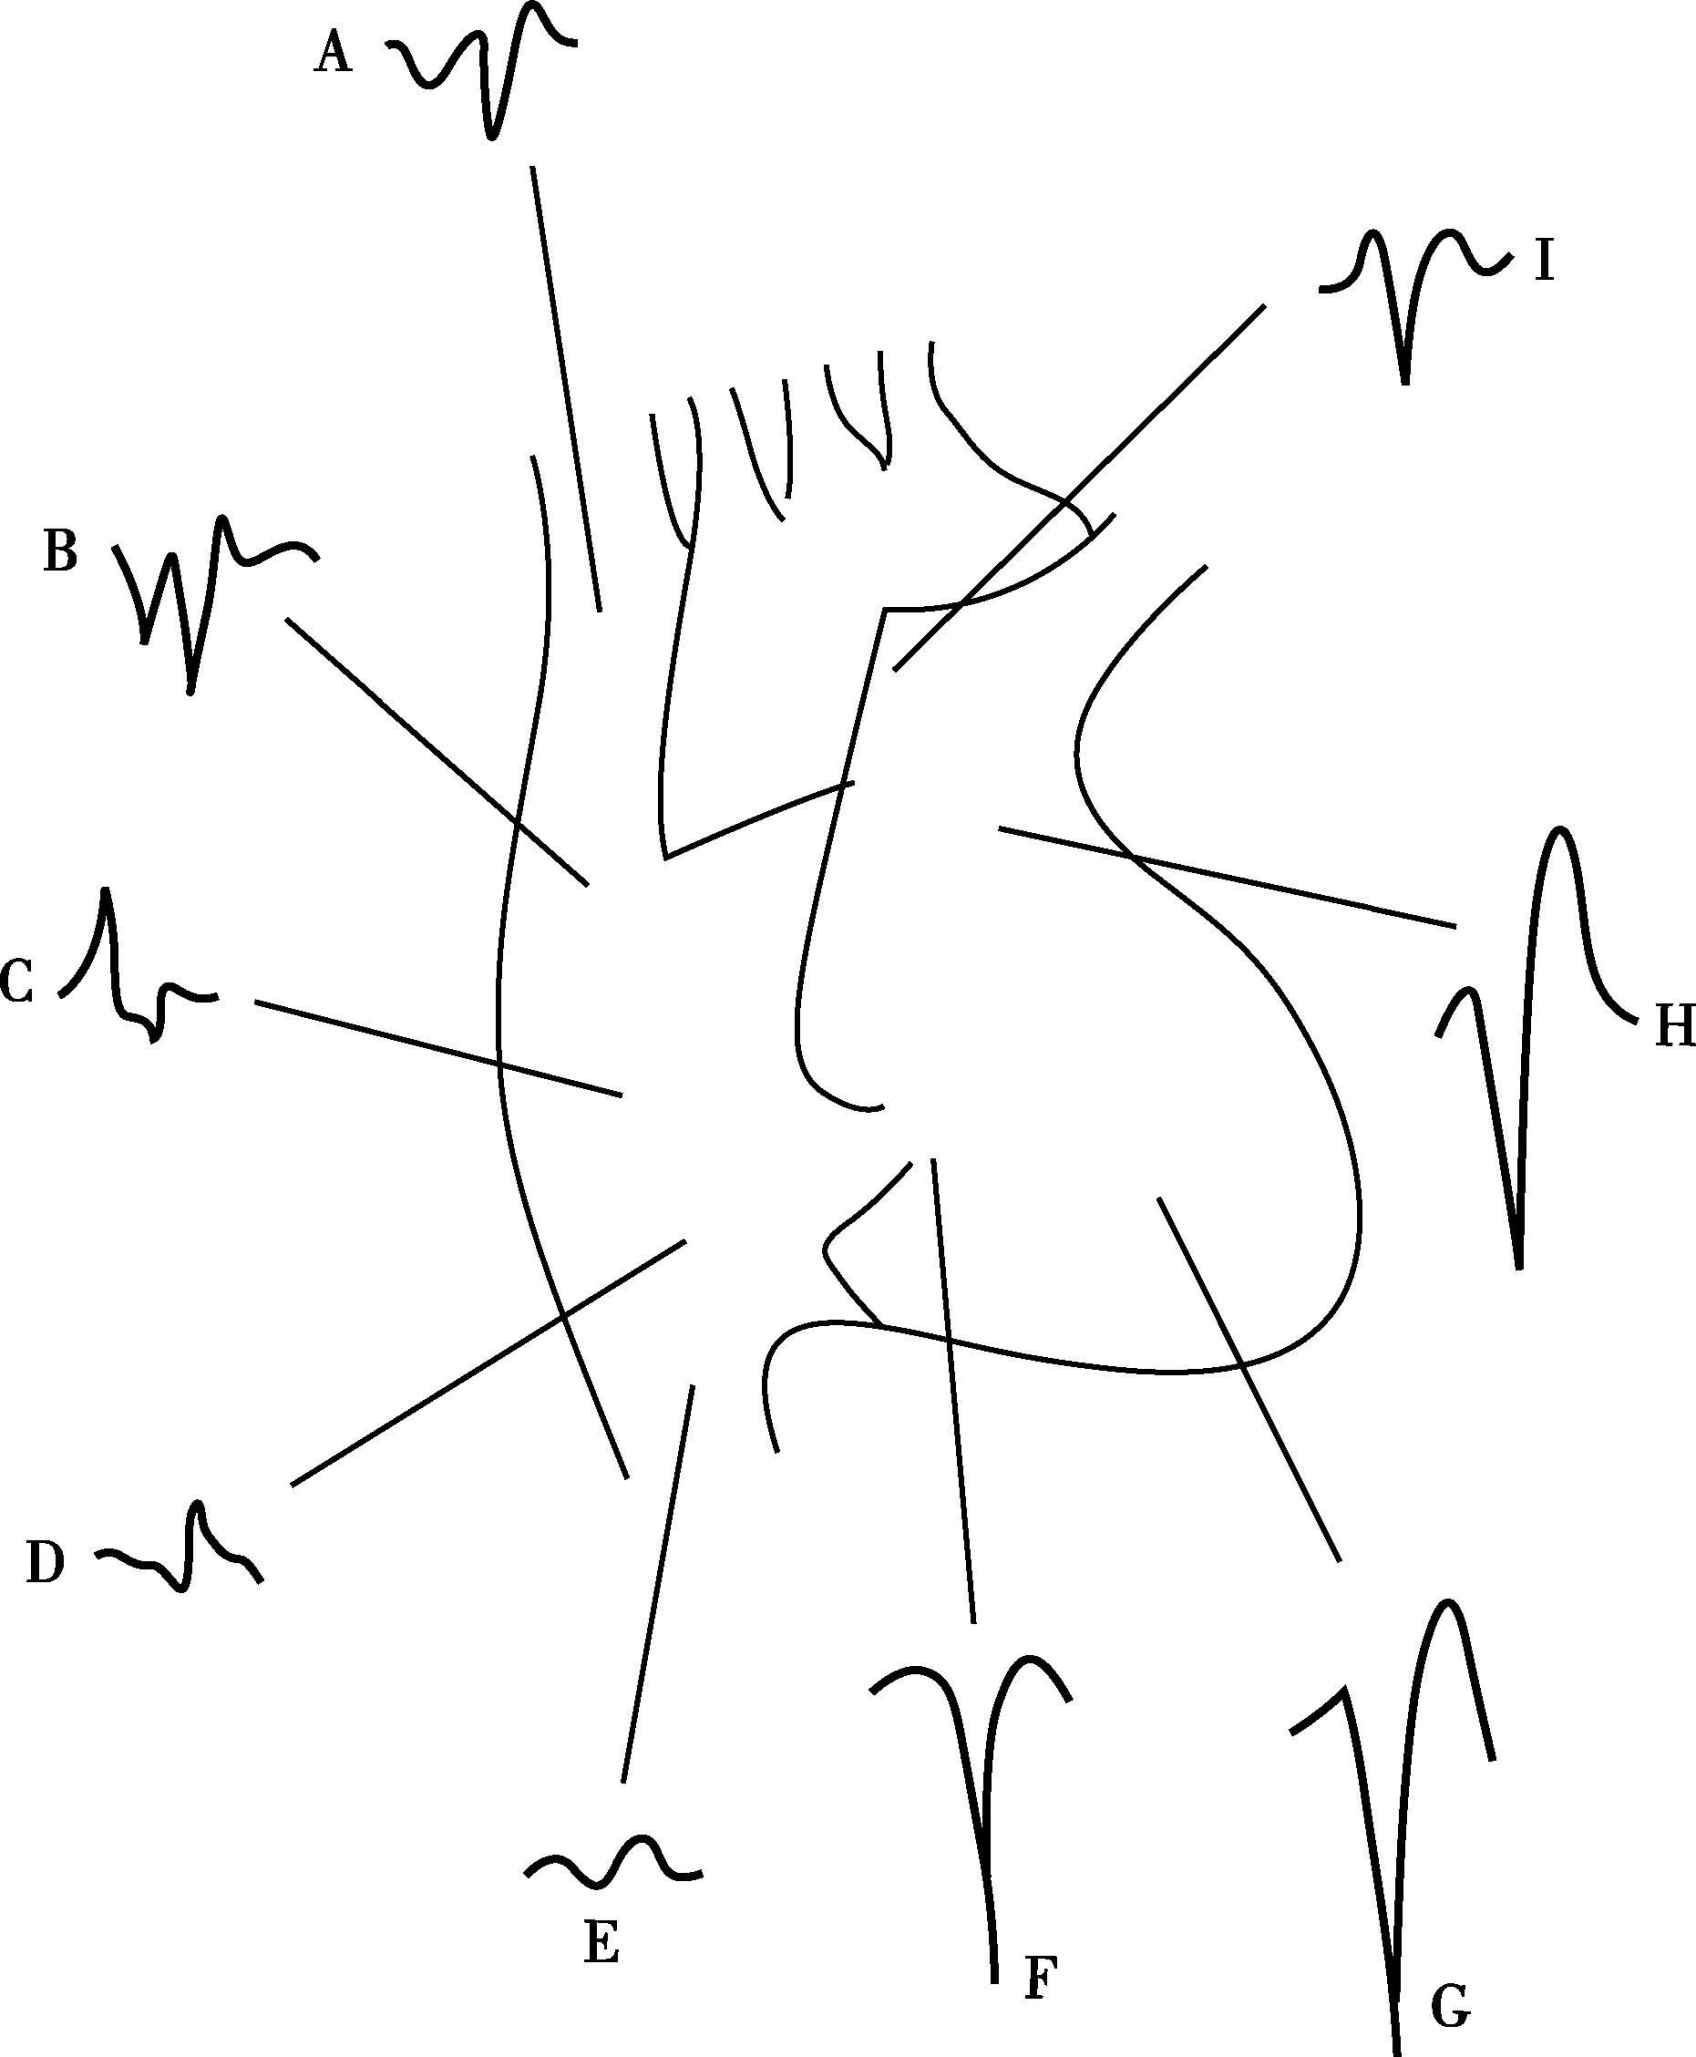
\includegraphics[width=3.09375in,height=3.76042in]{./images/Image00522.jpg}
 \captionsetup{justification=centering}
 \caption{上腔静脉(A);右房上、中、下部(B、C、D);右室流入道、中部、流出道(F、G、H);主肺动脉(I);下腔静脉(E)}
 \label{fig138-1}
  \end{figure} 

\begin{figure}[!htbp]
 \centering
 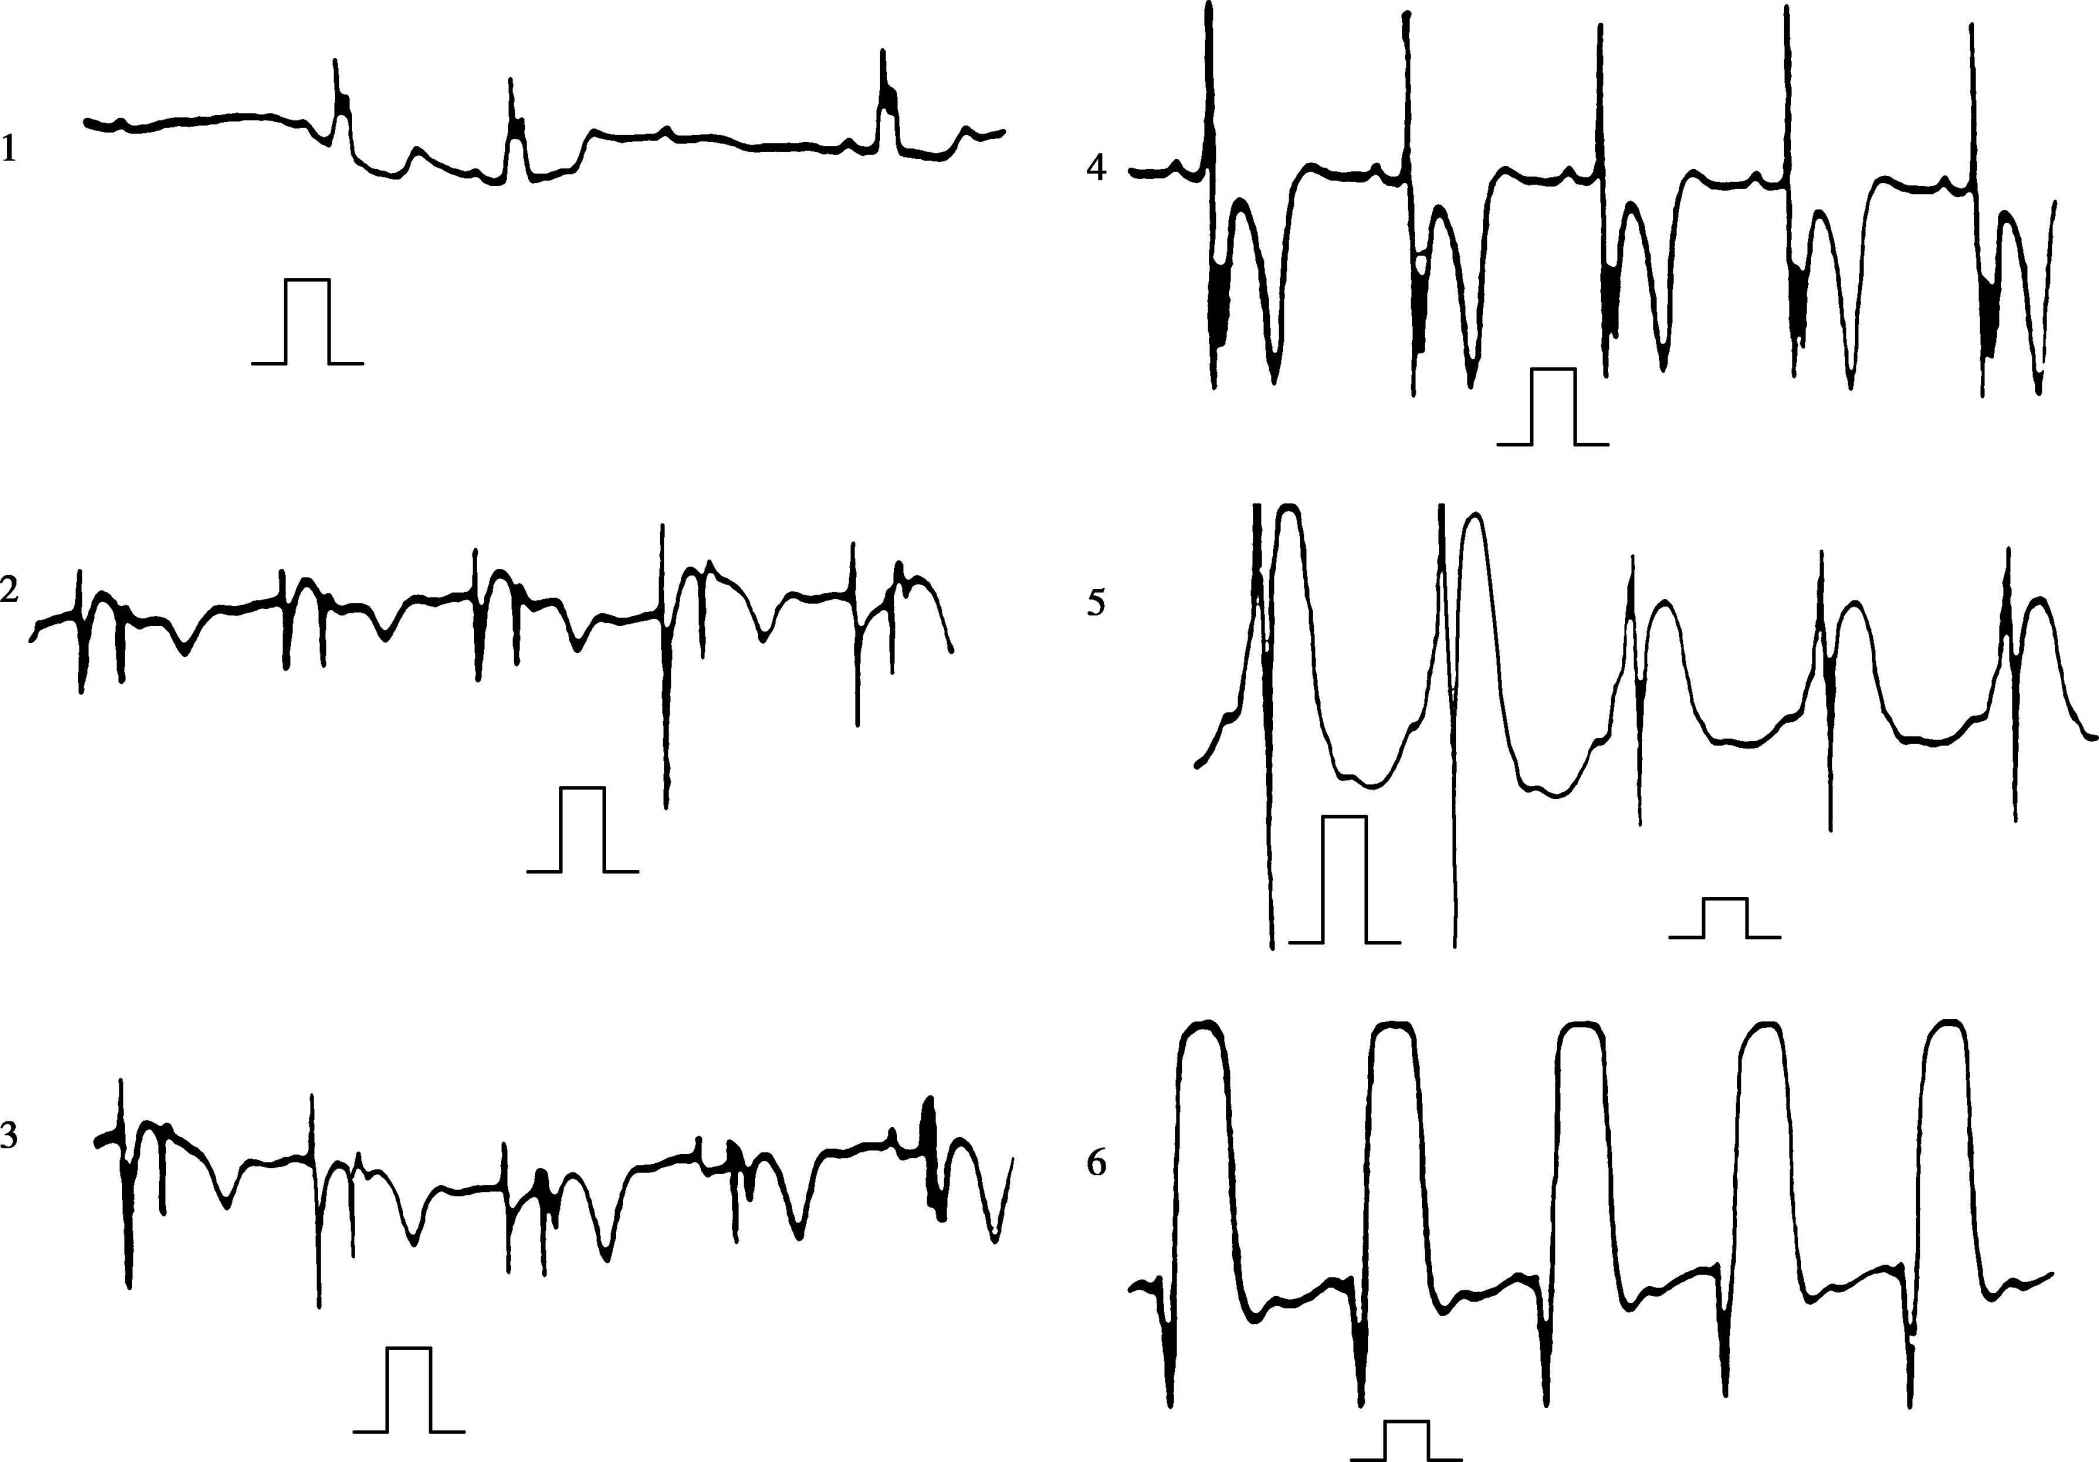
\includegraphics[width=5.95833in,height=4.14583in]{./images/Image00523.jpg}
 \captionsetup{justification=centering}
 \caption{心内导管指引导丝定位}
 \label{fig138-2}
  \end{figure} 

随着电极导管在心脏内的移动,可显示不同部位的心电图波形。1.二度AVB;2.电极位于右心房,P波较QRS波群大;3.后段:进入下腔静脉P波振幅小于QRS波;4.电极通过三尖瓣后进入右心室,QRS波增大,P波很小,T波倒置深;5.电极接触到心内膜,ST段上抬,心室波振幅为6mV;6.电极导丝对心内膜加压,则心电振幅增大,ST段明显抬高

①穿刺时如抽出血液呈鲜红色,或去除注射器后有搏动性的血液从针内流出,则提示误入锁骨下动脉,应即刻拔除针头,局部按压数分钟。②穿刺时如有疼痛和感觉异常并放射至手臂,则可能穿刺到臂丛神经处,亦应拔出针头。③如有空气吸出,提示可能穿入胸腔,应立即拔出针头,并密切观察有无气胸的症状和体征。④导入器的扩张管和外套管如不能插入锁骨下静脉,则提示锁骨和第一肋骨间隙较窄,可改在稍外侧处重新穿刺。⑤极少数患者的锁骨S形弧度较弯曲而又明显前凸,锁骨和第一肋骨没有间隙,亦可在稍外侧穿刺。⑥锁骨下静脉的压力较低,约为0~11.25mmHg,吸气时可为负压,因此在更换接头、去除注射器或针头及插入电极时,均需取头低脚高位,让静脉血缓缓流出,或应嘱患者呼气或处于呼气后的屏气状态,并应迅速操作,以免吸入空气,发生气栓。⑦插入“J”字形指引钢丝(导入静脉扩张管)时,宜将钢丝的弯头指向下肢,患者头转向导线插入侧,以利向下迅速进入上腔静脉,避免误入颈静脉。⑧从外套管插入电极时,应将电极前端的弯度方向指向下肢。⑨作起搏时的体表心电图Ⅰ、Ⅲ和V\textsubscript{1}
导联,可估计电极在心腔内的大致位置(表\ref{tab138-1})。⑩电极固定后,须将电极内指引钢丝拔除,否则太硬,可引起心肌穿孔。

\subparagraph{评价}

此方法对技术和经验要求较高,操作需花费一定时间,不适于心脏骤停、心室静止和电-机械分离等情况。但是,本法起搏稳定、可靠,对于非致命性的缓慢性心律失常价值较高。

\subparagraph{并发症}

①气胸:由穿刺针误入胸腔引起。少量气胸不必特殊处理,如为张力性气胸,应作紧急处理。②血胸:如血管损伤且流到胸腔则可致血胸,单纯的血胸少见,常为血气胸,必要时应会同胸科医生积极处理。③误入锁骨下动脉:可见鲜红的搏动性血液喷出。只要拔出针头,局部压迫即可;如已插入穿刺鞘者,不要贸然拔出,需请胸外科医师会诊一起处理,以防产生灾难性后果。④锁骨下动静脉瘘:常由于进针太深,穿过静脉和动脉,形成通道,较少见,必要时需作修补术。⑤空气栓塞:发生率<
1\%。因为胸腔在吸气时负压,可在穿刺或插入电极的过程中吸入空气形成肺动脉气栓。预防的方法是取头低脚高位,穿刺后最好始终有静脉血缓缓流出,或嘱患者在呼气状态下屏气。⑥其他少见的并发症:损伤迷走神经和喉返神经、血栓形成、胸导管损伤、皮下气肿及臂丛神经损伤等。⑦局部出血。⑧心肌穿孔。⑨心律失常。

\hypertarget{text00375.htmlux5cux23CHP16-5-3-3}{}
(三) 经食管起搏

由于食管紧贴心脏
,临床可以通过食管电极来起搏心脏,但是起搏脉冲幅度较心腔内起搏为高。

\subparagraph{设备要求}

体外临时心脏起搏器、普通食管电极或食管球囊电极、心电图机、心电监护仪。

\subparagraph{操作步骤}

①清醒患者咽部喷丁卡因表面麻醉,昏迷患者可借助喉头镜插入电极;②由鼻腔或口腔插入电极导管,到达30~40cm时,记录心电图,了解食管电极的位置,根据需要,选择心房或心室作为起搏点;③设置临时起搏器参数:VVI方式、频率70~80次/分、输出电压10V(或输出电流10mA)、脉宽5毫秒、感知灵敏度2.5mV;④连接电极与起搏器,观察起搏心电图,测试起搏阈值、阻抗和R波高度等参数后,固定电极。

\subparagraph{评价}

经食管起搏无创伤,电极容易放置,能迅速起搏,但在清醒患者因食管脉冲刺激,可能出现恶心、呕吐等不适,而且起搏稳定性不及心内起搏方式。

\hypertarget{text00375.htmlux5cux23CHP16-5-3-4}{}
(四) 经气管起搏

气管和食管一样
,与心脏邻近,把电极送至气管分叉以下,即靠近左心房中部,可以用于紧急心脏起搏。

\subparagraph{设备要求}

体外临时心脏起搏器、普通气管电极或气管球囊电极、心电图机、心电监护仪。

\subparagraph{操作步骤}

①昏迷患者可借助喉头镜,在气管插管同时,将起搏电极插入气管分叉以下;②记录心电图,了解气管电极的位置;③设置临时起搏器参数:VVI方式、频率70~80次/分、输出电压10V(或输出电流10mA)、脉宽5ms、感知灵敏度2.5mV;④连接电极与起搏器,观察起搏心电图,测试起搏阈值、阻抗和R波高度等参数后,固定电极。

\subparagraph{评价}

经气管起搏适用于昏迷患者,可以兼顾心肺复苏,但是患者清醒后不能耐受气管刺激,仅可作为过渡治疗。

\hypertarget{text00375.htmlux5cux23CHP16-5-3-5}{}
(五) 经皮肤起搏

又称为无创伤性临时起搏
,方法是将2个电极放置在胸壁皮肤上,阴极电极位于心尖部,采用较大的输出脉冲幅度起搏心脏。

\subparagraph{设备要求}

起搏除颤仪、皮肤电极、心电监护仪。

\subparagraph{操作步骤}

\begin{table}[htbp]
\centering
\caption{心室不同部位起搏的 QRS波及心电轴类型}
\label{tab138-1}
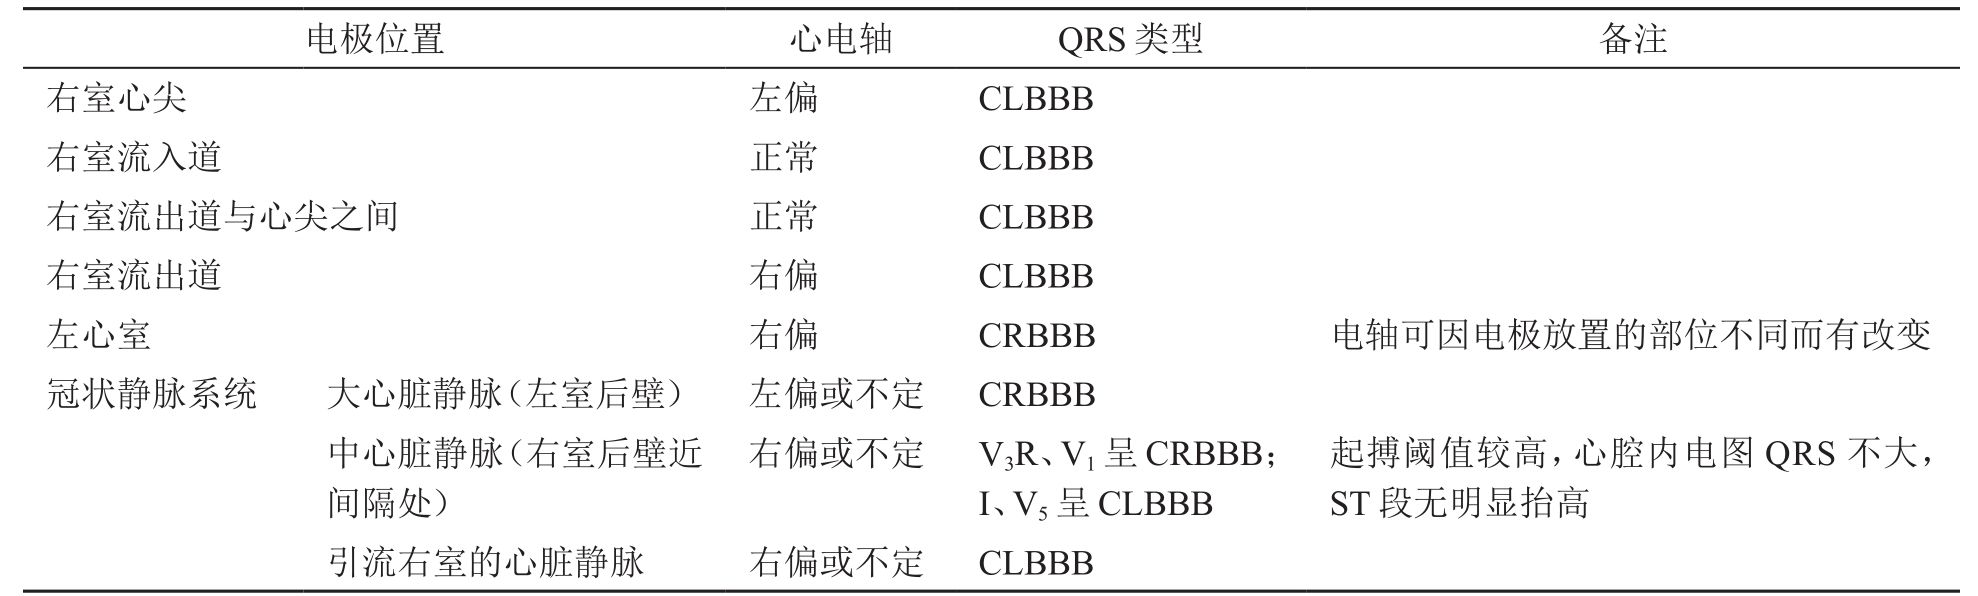
\includegraphics[width=6.58333in,height=1.97917in]{./images/Image00524.jpg}
\end{table}

①电极贴附:阳极位于左肩胛骨下角和脊柱间,阴极位于心前区;②连接带示波显示的起搏除颤仪和心电监护设备;③电极与起搏除颤仪连接,并接好地线;④设置临时起搏器参数:VVI或VOO方式、频率70~80次/分、输出电压10V;⑤开始起搏:电压由10V开始,逐渐增加至能起搏心脏,即为起搏阈值,然后再增加输出电压10\%,以确保安全可靠的恒定起搏。

\subparagraph{评价}

在不具备经皮穿刺心内膜、心肌起搏和经静脉起搏条件时,经皮肤起搏能迅速起搏心脏。由于电刺激强度大,清醒患者常不能耐受,最好能在起搏成功,患者复苏后,迅速建立经静脉起搏,保证安全有效的心脏起搏。

\hypertarget{text00375.htmlux5cux23CHP16-5-3-6}{}
(六) 开胸心外膜或心肌起搏

紧急心脏起搏多采用以上几种方法,在开胸手术或开胸心脏按压时,可采用本法。

\subparagraph{设备要求}

体外临时心脏起搏器、心外膜电极或钢丝钩状电极、心电监护仪。

\subparagraph{操作步骤}

①直接将钢丝电极插入心肌,或将心外膜电极缝合固定于心外膜;②设置临时起搏器参数:VVI方式、频率70~80次/分、输出电压5V(或输出电流10mA)、脉宽1.5ms、感知灵敏度2.5mV;③连接电极与起搏器,观察起搏心电图,测试起搏阈值、阻抗和R波高度等参数后,固定电极。

\subparagraph{评价}

该法起搏效果可靠,但是创伤性较大,仅限于已经开胸的患者。

\subsubsection{心室有效起搏的判断}

心脏是否有效起搏,是判断起搏成功与否的重要标志。至于患者是否存活,则与基础病变有关,不能单纯根据患者是否存活说明心脏起搏的有效与否。心室有效起搏在心电图上必须具备三个条件:①有一脉冲刺激信号。②随后有一个畸形而宽大的QRS波。③其后有一个倒置的T波。如没有T波,则脉冲刺激信号后可能并不是畸形的QRS波,而是脉冲电流的电位衰减曲线。

\subsubsection{紧急床边心脏起搏的选择}

心脏骤停、严重的窦性停搏或三度AVB致频发阿-斯综合征者,宜行经皮穿刺心内膜或心肌起搏;待病情稳定后,立即过渡为经左锁骨下静脉心内膜起搏;若无条件的单位,可送上级医院进一步治疗。若病窦综合征或AVB患者,应用异丙肾上腺素尚能维持生存者(室率稳定大于40~50次/分钟),宜直接行经左锁骨下静脉心内膜起搏。

\protect\hypertarget{text00376.html}{}{}

\chapter{床旁血流动力学监测}

血流动力学监测是对危重患者进行救治时的一种非常重要的心功能监测手段,临床上分为有创和无创两类,以间断或持续的方式进行床旁监测。其目的是:①通过右心腔压力、肺动脉压、肺毛细血管楔嵌压(PCWP)、动脉压与心输出量等测定结果,了解低排、低血压、休克及心室充盈压改变的原因与程度。②诊断急性心肌梗死并发室间隔穿孔、急性二尖瓣功能不全、右室心肌梗死与心脏压塞等。③监测补液、扩血管药、正性肌力药与升压药疗效,指导治疗。

\subsubsection{血流动力学监测的适应证}

血流动力学监测的适应证是:①有助于确诊某些危重情况,如急性心肌梗死并发室间隔缺损或二尖瓣关闭不全,鉴别心源性与非心源性肺水肿,急性下壁心肌梗死伴右心室心肌梗死,肺动脉栓塞,难以心电图确诊的心肌缺血(如合并左束支阻滞)。②病情复杂且不稳定,而其他检查(临床症状、X线拍片或容量负荷试验)难以提供可靠资料时,包括复杂心脏情况如急性心肌梗死并发低血压,显著血流动力功能不稳定(需要正性肌力药、血管活性药或机械辅助治疗时)及心功能不全,不稳定心绞痛应用硝酸甘油或其他血管活性药静脉滴注治疗,循环血量或心血管状态不明确而又不宜进行利尿或容量负荷治疗,以及伴低血压的右室心肌梗死患者。③心脏病患者合并其他内科情况,如胃肠道大量出血、脓毒血症、呼吸衰竭、肾功能衰竭、胰腺炎、血液透析等。④心脏病患者合并外科情况,尤其是有反复发作或新近发作的心肌缺血,或心室功能不全、心律失常,或液体与电解质失衡可能时,如心脏手术(多个心瓣置换、合并严重肺部疾病、冠脉旁路手术、室壁瘤切除等),大血管手术(主动脉夹层、胸或腹主动脉瘤切除),前列腺切除,严重烧伤,多发外伤。⑤心脏病患者合并产科高危情况(妊娠毒血症或胎盘早期剥离等)。⑥评价新药对心血管系统的作用,并保证用药安全。

\subsubsection{有创血流动力学监测的基本设备}

1.Swan-Ganz导管 即气囊漂浮导管(balloon flotation
catheter)。早期的气囊漂浮导管有3个内腔,简称三腔管。导管顶端和距顶端20~30cm处开孔,近顶端处还有通气囊的开孔,3处开孔经相互隔离的管腔分别开口于导管尾端。在距导管顶端4cm处安装热敏电阻,由导线经另一隔离的管腔与尾端接头相通的气囊漂浮导管,称为四腔漂浮导管。在距四腔导管顶端25~26cm处各安装1个环状电极,或在17~18cm处再各装环状电极1个,分别由导线经隔绝的管腔通向尾端的气囊漂浮导管,称为多功能气囊漂浮导管。3种漂浮导管的共同特点为当导管经静脉进入心腔后,充气的气囊有导向作用,使导管顺血流方向漂浮,在较短时间内自动地由右房经右室进入肺动脉,并嵌顿在肺动脉较小分支内,提供床旁监测右房、右室、肺动脉和肺楔嵌压等指标的可能。充气的气囊将导管的顶端包围,从而显著减轻或避免了导管顶端碰撞右室壁引起的室性心律失常。四腔管的热敏电极提供了用温度稀释法监测每搏血量与心排血指数的可能。多功能漂浮导管在上述基础上外加2对电极,经适当滤波后可分别监测右房与右室腔内心电图,因而应用同一导管不仅能监测心腔内压力和心排血指数,还有可能同时监测心率和心律。必要时还可应用该组电极进行右房、右室或房室顺序心脏起搏,治疗缓慢或快速心律失常。

2.中心静脉导管 有单腔、双腔和三腔之分。

3.动脉导管。

4.压力换能器
一端与监测仪相连,另一端通过三通开关与漂浮导管第一管腔相连。通常安放的位置与患者的右心房在同一水平高度。

5.床旁监测仪
分别与压力换能器和心电图输入导联线相连。能显示和记录压力曲线和读数,显示和记录心电图信号。

6.三通开关及延长管
一端接漂浮导管第一管腔,另一端接肝素液(50mg肝素加入500ml等渗液体中),再一端与压力换能器连接。非测压时肝素液和第一管腔相通,持续滴入肝素液以防管腔内凝血。测压时则使第一管腔与压力换能器相通。

7.其他 备用抢救设备和药品,心输出量计算器等。

\subsubsection{动脉压(IBP)}

有创动脉血压监测是临床上最常用的直接测压方法,也是监测动脉压最为精确的一种技术。

\hypertarget{text00376.htmlux5cux23CHP16-6-3-1}{}
(一) 适应证和禁忌证

适应证包括:①体外循环下的心内手术,大血管手术。②血流动力学不稳定(如无创测压有困难),即使压力低于30~40mmHg,仍可准确测量。③需频繁采集动脉血标本。

禁忌证包括:①Allen试验阳性者禁止行同侧桡动脉穿刺。②局部有皮肤感染。③存在凝血功能障碍。

\hypertarget{text00376.htmlux5cux23CHP16-6-3-2}{}
(二) 操作步骤与注意事项

常用的穿刺部位有桡动脉
、尺动脉、足背动脉、肱动脉、股动脉、腋动脉。一般首选桡动脉,因为容易置管,相应并发症少,但患者在置管前必须进行Allen试验。具体方法:将患者一侧手臂抬高于心脏水平,握拳,术者用拇指按在前臂尺动脉上,另一拇指按压桡动脉上,同时加压5秒,并放低手臂松开拳头,松开压迫的尺动脉,如掌部、手指在15秒内恢复红色,为Allen试验阴性,如不能在15秒内恢复红色,说明主要依靠桡动脉灌注,为Allen试验阳性。

1.动脉压测量
应先确定压力零点水平。多将压力换能器固定在患者右心房中部水平线,即选择第4肋间隙腋中线水平作为零点水平。

2.换能器与装有生理盐水或肝素盐水的加压袋相连接
,以3ml/s的速度连续冲洗管道,避免导管尖端凝血块形成。

3.零点校正
方法:①关闭通向动脉导管的三通,打开冲洗装置,使管道充满液体;②打开换能器排气孔;③按压一次监测仪上的零点校正开关,使监测仪上的压力曲线及读数均回到零位;④零校正完成,关闭排气孔。

4.打开与血管相连的三通开关,监测仪上即显示压力曲线和读数。

5.影响动脉压监测准确性的因素有
①动脉导管的固定不当或堵塞,表现为动脉波形变化,收缩压下降,波形变平坦。应充分可靠地固定导管。②管道内的气泡可以降低压力传递的敏感性,降低数值,应排空管道内的气泡。③管道应有一定的硬度,尽可能少的三通开关和尽可能短的动脉延长管以保证压力波形正确传递,提高测定值的精确性。

6.动脉压监测的临床意义
动脉压受心输出量、循环血容量、外周血管阻力、血管壁弹性和血液黏滞度等因素的影响,反映循环功能的一个侧面。动脉压分为收缩压(SBP),主要由心肌收缩力和心输出量决定,其作用是克服各脏器的临界关闭压;舒张压(DBP),主要由外周血管阻力决定,作用在于维持冠状动脉灌注压。平均动脉压(MAP)公式:MAP
=
1/3(收缩压−舒张压)+舒张压,在评估重要器官灌注压时最常用。脉压是收缩压和舒张压之差,反映每搏量及外周血管阻力,低于30mmHg的脉压常见于低血容量、心动过速、主动脉狭窄、缩窄性心包炎、胸腔积液和腹水,脉压增大可能是主动脉反流、甲状腺毒症、动脉导管未闭、动静脉瘘。

\subsubsection{中心静脉压}

中心静脉压(CVP)是位于胸腔内上、下腔静脉或右心房内的压力,它是评估血容量、右心前负荷及右心功能的重要指标,临床抢救危重患者中被广泛地应用。

\hypertarget{text00376.htmlux5cux23CHP16-6-4-1}{}
(一) 适应证和禁忌证

主要适应证包括
:①休克(主要是失血性和感染性休克)。②心功能不全或心衰。③需要大量输血和输液。

对有严重凝血功能障碍的患者是相对禁忌证,血气胸患者避免行颈内或锁骨下静脉穿刺。

\hypertarget{text00376.htmlux5cux23CHP16-6-4-2}{}
(二) 操作步骤与注意事项

通过颈内静脉
、锁骨下静脉、颈外静脉、头静脉、腋静脉、股静脉可以提供中心静脉通路。如果穿刺时用手提式二维超声显像,更可以明确中心静脉解剖位置和血流情况,提高置管的准确性,减少并发症。

\subparagraph{中心静脉压测量方法}

一般有两种:①换能器测压,通过装满液体的管道将血管腔与压力换能器相连接而测得,在监测仪上显示出静脉压力曲线和读数。②水压力计测压,因中心静脉压是低压系统,可用水压力计直接测压,应用中心静脉测量标尺,垂直固定于架子上,其零点位置定于第4肋间隙腋中线,测压管道通过三通开关与中心静脉导管相连。

\subparagraph{影响中心静脉压测量的因素}

①导管位置:中心静脉压导管置入的最佳位置应该是上腔静脉与右心房连接处的血管内,但大部分导管置于上腔静脉内。②零点:以右心房中部水平线为准,体表投射位为腋中线第4肋间隙水平线,患者体位改变时要及时调整。③气道内正压:胸腔压是经心包和腔静脉壁传递的,自主呼吸时,吸气降低CVP,呼气升高CVP,而在机械通气时正好相反。CVP升高的程度取决于肺的顺应性和血容量,因此,最好在呼吸周期的同一时期测量和比较,一般在呼气末期。应用呼气末正压时(PEEP),正压会传递到右心房,引起静脉回流的减少和CVP升高;而PEEP对CVP的影响也随着肺顺应性和血容量不同而不同。建议测CVP时在病情允许的情况下,短暂关闭PEEP。④导管的扭曲、受压、血管堵塞均会影响测得的值。

\subparagraph{中心静脉压监测的临床意义}

①CVP降低同时:BP升高,心脏实际功能增强;BP降低,血容量减少或静脉回流阻力增加。②CVP升高同时:BP升高,血容量增多或静脉回流阻力下降;BP降低,心脏实际功能降低。

\subsubsection{气囊漂浮导管}

\hypertarget{text00376.htmlux5cux23CHP16-6-5-1}{}
(一) 适应证和禁忌证

肺动脉压监测对急性心肌梗死伴有如下情况者可能获益:①不易通过补液纠正的低血压。②充血性心力衰竭存在时的低血压。③血流动力学损害严重,需静脉使用缩血管剂或扩血管剂或主动脉内气囊反搏术。④机械损害或可疑机械损害,如心脏压塞、严重二尖瓣关闭不全、室间隔穿孔。

禁忌证同中心静脉压监测。

\hypertarget{text00376.htmlux5cux23CHP16-6-5-2}{}
(二) 操作步骤与注意事项

1.检查漂浮导管
①检查气囊的完整性:向气囊内注入1~1.5ml气体,看气囊是否充气、有无偏心等,然后置入无菌生理盐水中,观察其完整性。②检查导管是否通畅:可用肝素生理盐水冲洗管腔,然后关闭三通开关,保证空气绝对不能进入管腔。

2.确定导管插入方法
有静脉切开法和静脉穿刺法两种,以后者较为简单,易为患者接受。不同部位插管之比较见表\ref{tab139-1}。

3.确定导管进入的部位
导管顶端插至右心房所需要送入导管的长度与导管插入不同部位的浅表静脉有关(表\ref{tab139-2})。

4.当导管顶端进入右心房后,将气囊充气,立即将开关关闭,使气体保持在气囊内。应注意注入气体总量不能超过气囊的容量,以防止气囊破裂。将导管末端连接测压器,以观察压力的变化,若监测仪所示的压力波形随呼吸运动而明显移动,则证实已达右心房。此时静注利多卡因1mg/kg,3分钟后再送导管漂浮入右心室,可明显减少导管通过时室性心律失常的发生率。气囊充气后在血液中漂浮前进,一般能在1分钟内即可以从右心房经右心室进入肺动脉,最后可到达肺动脉分支楔嵌的位置。

\begin{table}[htbp]
\centering
\caption{不同部位插管比较}
\label{tab139-1}
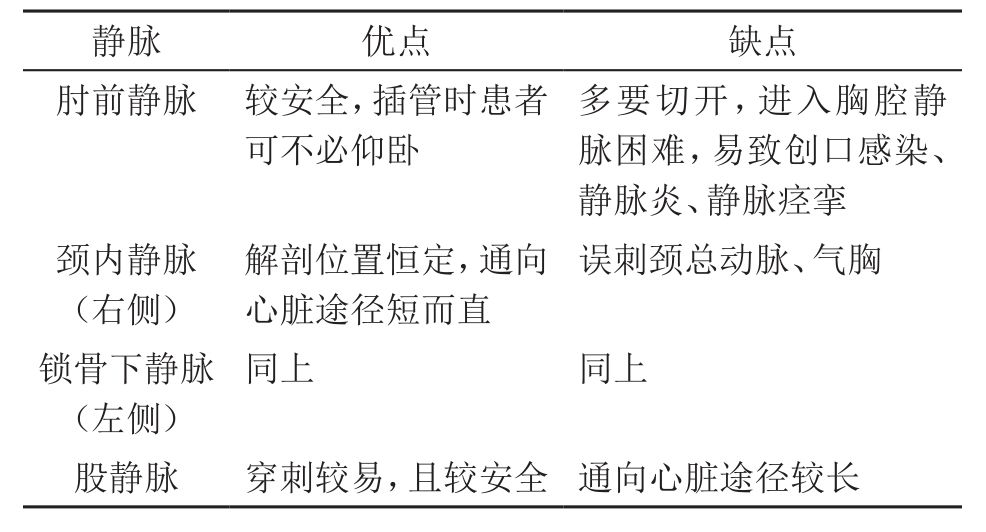
\includegraphics[width=3.27083in,height=1.76042in]{./images/Image00525.jpg}
\end{table}

\begin{table}[htbp]
\centering
\caption{漂浮导管插入途径及至右心房的距离}
\label{tab139-2}
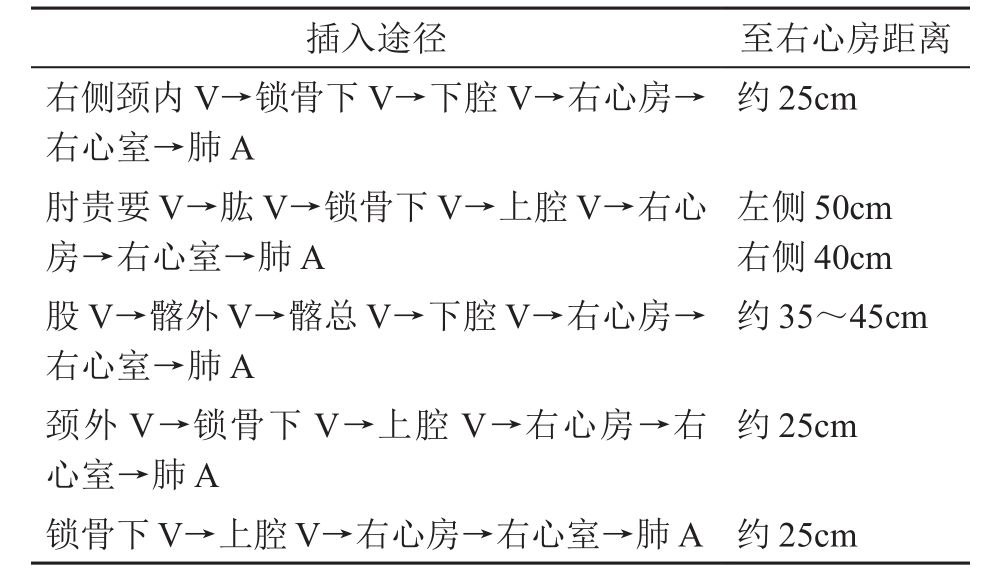
\includegraphics[width=3.28125in,height=1.94792in]{./images/Image00526.jpg}
\end{table}

5.当漂浮导管插入右心房时
,监测仪显示右心房压力曲线,此时总压力波幅(正常)约4.0mmHg;进入右心室时,显示右心室压力曲线,收缩压较右房增高;入肺动脉时,出现肺动脉压力曲线,舒张压较右室增高而收缩压不变;导管漂浮前进至充气的气囊堵塞肺动脉分支时,可见压力波幅仅2.0mmHg,为具有3个波峰的压力波,即肺毛细血管楔嵌压(PCWP),相当于导管顶端与肺毛细血管、肺静脉和左房间形成的静态血柱的压力,此时,肺动脉压力曲线消失,将气囊放气后,肺动脉压力曲线再度出现,说明导管位置正确。如气囊充气时<
1ml已能记录到PCWP,则指示气囊进入肺小动脉,可能太深了;如充气量>
1.5ml才显示PCWP则提示气囊进入肺小动脉的深度不够。

6.应用热稀释法测定心排出量
应用四腔气囊漂浮导管连接心排出量测定仪,可间断监测心排出量及心脏指数。事先准备冰冻无菌的5\%葡萄糖液1瓶,插入心排出量测定仪的温度测定探头,与测定仪连接。再将已送达肺动脉的气囊漂浮导管尾端的热敏电阻接头与测定仪连接,测定仪的电脑装置即能连续显示注射液温度和患者的血温。启动测定仪,用无菌注射器抽取冰葡萄糖液5ml,立即用最快速度自导管尾端右房孔开口推入(短于4秒)。冰注射液随血液进入右室,与血充分混合,凉血于心室心缩时进入肺动脉,该处热敏电阻测得的系列血温改变,由心排出量测定仪绘制成温度-时间曲线,测定仪同时显示心排出量和(或)心脏指数。2分钟后可重复测定,一般取3次测定值的均值作为心排出量和(或)心脏指数值。

7.在某些大心脏(如右心扩大)、急性心排出量降低、三尖瓣病变和肺动脉高压等患者中,有时插入导管较困难。此时嘱患者深吸气,作Valsalva动作,用5~10ml冰盐水冲洗导管或在导管内插入细引导钢丝,使导管变硬,均有助于插入至肺动脉。一旦导管插妥,导管鞘退出,导管用缝线固定,覆盖无菌敷料。

8.导管保留时间依病情而定
,一般1~4天。在导管保留期间,导管心房孔与肺动脉孔要用含肝素的液体缓慢持续点滴,以防导管内凝血。每次测定肺楔嵌压后务必立即放气,以防肺血管受损或肺梗死。在导管保留期间可酌情使用抗生素以预防感染。

\hypertarget{text00376.htmlux5cux23CHP16-6-5-3}{}
(三) 并发症及其防治

1.气囊破裂
①原因:多见于肺动脉高压患者或导管重复多次使用及气囊充气过多的情况。当充气后不再能复原就应怀疑气囊破裂,可注射1ml盐水,不能回抽或回抽有血就可以证实,应立即拔出导管。②预防:插管前仔细检查导管,应注意充气量不超过1.5ml,充气速度不宜过快。

2.心律失常
系导管前端接触到心内膜所致,多见室性期前收缩。因此,插入导管前可预防性地注入利多卡因;在插管过程中出现心律失常时,应改变导管位置,必要时给予抗心律失常药物。

3.穿刺部位或全身感染及静脉炎
①原因:消毒不严,无菌操作技术不佳。②预防:严格消毒,注意无菌操作,定期更换敷料。置管时间尽量缩短,一旦发生感染,要积极应用抗生素治疗,必要时予以拔管。

4.导管扭曲打结
系导管软或插入过长所致。当过多的导管进入但仍未达预定的导管位置时应高度怀疑此种可能。插管前应注意选择导管,应避免导管插入过长。发生扭曲时,应退出或调换导管;打结应将导管轻送轻抽使之松开。

5.气胸
在锁骨下静脉插管时,较易因误伤胸膜而致气胸。注意进针部位与针尖方向可预防发生。

6.穿刺部位渗血、出血、血肿形成。

7.血栓形成
①置管时间过长,如用18G导管置管1~3天血栓发生率25\%,20G的发生率为10\%,使用22G能进一步减少血栓发生率。②置管过程容易损伤血管内膜,阻碍导管周围的血流而形成血栓。③导管质量:使用聚四氟乙烯导管比用聚乙烯导管发生血栓的可能性小得多。④不同部位动脉穿刺血栓发生率:桡动脉17\%,肱动脉44\%,足背动脉发生率较低。

8.肺栓塞
①原因:栓子多来自导管顶端的血凝块,以及冲洗时管道内的气栓等。漂浮导管在肺动脉中多次移动,气囊过度扩张等均可促使血栓形成并引起栓塞。②预防:气囊应间断缓慢充气,充气量宜少,置管时间尽量缩短。对时间超过48小时者,可预防性应用抗凝剂。

\hypertarget{text00376.htmlux5cux23CHP16-6-5-4}{}
(四) 监测的指标

直接测定的指标包括周围动脉压
、右房压(RAP)、右室压(RVP)、肺动脉压(PAP)、肺毛细血管楔嵌压(PCWP)和心排出量(CO)。按公式可根据上述参数计算出平均动脉压(MAP)、心室每搏做功指数以及周围循环阻力、肺循环阻力等指标(表\ref{tab139-3})。此外,重复测定同一患者PCWP连续增高时的心排出量,可绘制以PCWP为横坐标、心排出量为纵坐标的该患者的心肌做功曲线,反映在后负荷不变条件下心肌的内在收缩功能。

\subparagraph{右房压(RAP)}

正常值为1~7mmHg,其中收缩压3~7mmHg,舒张压0~2mmHg。RAP升高见于右心衰竭、三尖瓣狭窄或关闭不全,以及任何可影响心室舒张期充盈的情况如缩窄性心包炎、心肌病、肺动脉高压、阵发性心动过速等。

\subparagraph{右室压(RVP)}

正常值:收缩压20~30mmHg,舒张终末压<
5mmHg。其增高的原因有:①任何原因引起的肺动脉高压。②肺动脉狭窄。③右室衰竭。④缩窄性心包炎。⑤右心室梗死。

\subparagraph{肺动脉压(PAP)和肺毛细血管楔嵌压(PCWP)}

PAP正常值为15~30/5~14mmHg,其升高见于左心衰竭、二尖瓣病变、慢性肺部疾病、肺动脉高压等。PCWP正常值为5~12mmHg,当>
18mmHg时为肯定升高,> 25~30mmHg则有肺水肿的可能;当<
8mmHg时常有左室充盈不足。根据心脏做功曲线,当PCWP在15~18mmHg时,左室做功最佳。PCWP在一定程度上反映了肺静脉压,由于肺动脉与左心房之间无瓣膜,且正常血管床的阻力低,故也能间接反映左心房压。在心室舒张末期,二尖瓣开放,肺静脉、左心房与左心室呈共同腔室,此时PCWP与左心室舒张终末压近似,故PCWP可作为反映左室舒张末期压(LVEDP)的指标,是了解左心室功能的确切指标(在无二尖瓣狭窄存在时)。肺动脉舒张压与PCWP密切相关,在无严重肺部病变的患者,肺动脉舒张压略高于PCWP,较稳定地高出后者1~4mmHg,因而常以连续肺动脉舒张压监测取代PCWP连续监测,以避免PCWP监测时充气的气囊长久楔嵌引起肺动脉分支管壁损伤甚至穿破,以及肺梗死等并发症。

\subsubsection{脉波指示剂连续心排出量监测(PiCCO)}

PiCCO(pulse indicator continous cardiac
output)是将肺热稀释法与动脉脉搏波形分析技术结合起来测定连续心排出量的一项微创血流动力学监测新技术。只需配置中心静脉及动脉导管,不需放置肺动脉导管。尤其是利用热稀释法能够连续测定胸腔内血容量(intrathoracic
blood volume, ITBV)及血管外肺水(extravascular lung
water,EVLW)这两个容量监测指标,可以更准确、及时的反映体内液体的变化。

\hypertarget{text00376.htmlux5cux23CHP16-6-6-1}{}
(一) 适应证

①血流动力学不稳定状态。②休克。③脓毒血症。④肺损伤。⑤多器官功能衰竭。

\hypertarget{text00376.htmlux5cux23CHP16-6-6-2}{}
(二) 操作步骤与注意事项

1.局麻下经右股动脉置入带温度传感器的
PiCCO动脉导管,经右侧颈内静脉或锁骨下静脉置入中心静脉导管,动静脉导管与PiCCO
plus监测仪相连接。确定第四肋腋中线水平后经与中心静脉导管相连的水温探头固定仓10秒恒速注入10ml生理盐水(2~5℃),经过上腔静脉→右心房→右心室→肺动脉→血管外肺水→肺静脉→左心房→左心室→升主动脉→腹主动脉→股动脉→PiCCO导管接收端,换能器校零。计算机将整个“热稀释”过程画出“热稀释”曲线,并自动对该曲线波形进行分析,得出一基本参数,然后结合PiCCO导管测得的股动脉压力波形,得出每搏心输出量、心脏指数、动脉压、血管外肺水、肺水指数。

2.换能器校零
置管后分别对股动脉换能器和中心静脉换能器校零。每8小时校零1次。方法:将换能器平腋中线第4肋,与大气相通,按监测仪校零键,直至数值归零,再转入三通开关使换能器与各导管相通,校零完成后可连续监测动脉血压和CVP。

3.定标 每8小时1次。定标前中心静脉停止输液30秒以上,经中心静脉内快速(<
8秒)注射盐水10~15ml,动脉导管尖端的热敏电阻测量温度下降的变化曲线,通过分析热稀释曲线计算得出CO。重复上述操作3次取平均值,得出定标值。应避免频繁测定,增加心脏负荷。

4.PiCCO参数测定
①连续监测的参数:每次心脏搏动的心排出量(PCCO)及指数(PCCI)、动脉压(AP)、心率(HR)、每搏量(SV)及指数(SVI)、每搏量变化(SVV)、外周血管阻力(SVR)及指数(SVRI);②利用热稀释法测定的参数:心排出量(CO)及指数(CI)、胸腔内血容量(ITBV)及指数(ITBI)、全心舒张末期容量(GEDV)及指数(GEDI)、血管外肺水(EVLW)及指数(ELWI)、心功能指数(CFI)、全心射血分数(GEF)、肺血管通透性指数(PVPI)。

\begin{table}[htbp]
\centering
\caption{血流动力学计算公式与正常值}
\label{tab139-3}
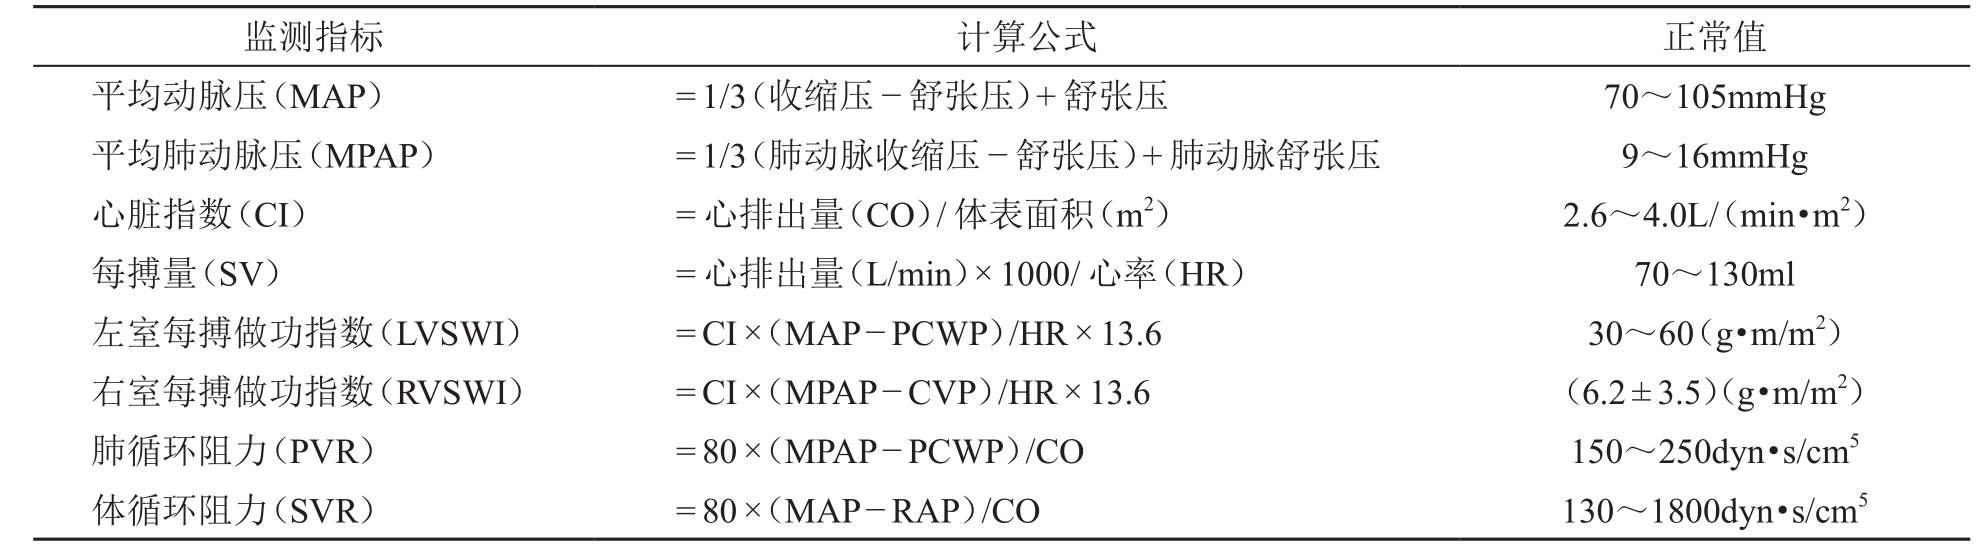
\includegraphics[width=6.59375in,height=1.84375in]{./images/Image00527.jpg}
\end{table}

5.PiCCO监测的临床意义
①心排出量(CO):反映心脏的输出功能,是组织供氧的保证。CO下降表示血容量不足或心功能不全,CO增高提示焦虑、运动、感染性休克等。②胸腔内血容量(ITBV):是由左右心腔舒张末期容量和肺血容量组成,因此与心腔充盈量密切相关,它不受机械通气的影响。包括四个腔室舒张末期容量的总和,即ITBV
=全心舒张末期容量(GEDV)+肺血容量(PBV)。参考值为850~100ml/m\textsuperscript{3}
。数值过高提示血容量过多,数值过低提示血容量不足。③血管外肺水(EVLW):包括细胞内液、间质液和肺泡内液,后两种过多造成肺水肿。因此可用于危重症患者肺水肿的监测。参考值为3.0~7.0ml/kg,增加提示有肺水肿的可能,可在床旁定量判断肺水肿的程度,对ARDS患者有特殊意义。

\subsubsection{无创血流动力学监测}

无创血流动力学的监测,因其安全、简便、无痛苦而在临床上得到广泛的应用,包括心率(HR)、无创血压(NIBP)、脉搏血氧饱和度(SpO\textsubscript{2}
)、心排出量(CO)等监测指标。在诸多监测参数中,CO的监测是最重要的参数之一。目前临床上无创监测心排出量的方法有:①心阻抗血流图;②食管超声心动图;③多普勒技术;④二氧化碳无创心排出量测定。

心阻抗血流图(impedance
cardiogram,ICG)是通过每一心动周期胸部电阻抗的变化,测定心血管功能。其基本原理是认为人体组织是一个导电性能良好的导电体,尤其是充满导电离子的血液系统。当直流电通过胸部组织时,人体产生电阻。人体的胸腔长度是恒定的,血流的电阻率为135~150Ω/cm,每次心搏时,主动脉的内径相应地改变,而主动脉内血流是胸部主要的导电介质,主动脉内径扩张导致胸部电阻R的变化。根据欧姆定律:电流I
=电压V/电阻R,可以测得电阻R的变化。可见,在导体长度不变的情况下,容积变化与阻抗R的变化密切相关。心阻抗血流图利用这一原理,采用高频(70Hz)、恒定、低强度(2.5mA)交流电通过胸部,探测胸部阻抗的变化,了解胸腔内血流情况。

目前临床上常用的心排出量监测仪有多种型号,诸如NCCOM2(noninvasive
continuous cardiac output
monitor)、NCCOM3、NCCOM3-R7、cardiodynamic监测仪等。监测仪在与患者相接时,局部皮肤要用酒精清洁干净,在颈根部和剑突水平放置4对8个电极时,相邻两个电极要相距5cm。电极必须用银-氯化银电极,这样可以得到较小的阻抗值,减少干扰。通过心排出量监测仪,可以测得多项血流动力学参数,如心率HR、每搏量(SR)、心排出量(CO)、射血速率指数(EVI),其反映心脏的收缩性;心室射血时间(VET),其表示机械收缩间期;胸腔体液指数(TFI),其反映肺泡间质和血管内液体分布;心脏指数(CI),反映全身血流和组织灌注状态;每搏指数(SI),反映心泵功能;舒张末期指数(EDI),反映前负荷;心收缩指数(IC),反映心室充盈和收缩性;加速度指数(ACI),反映不依赖前后负荷变化的心肌收缩功能;体循环血管阻力指数(SVRI),反映前后负荷变化;左心室每搏做功指数(LCWI),反映心室克服后负荷每搏做功能力;射血分数(EF),反映左心室容量排空的效应;以及平均动脉压(MAP)。

超声心动图监测(ultrasonic cardiogram echocardiogram
monitor,UCG)是利用高频超声波(2.5~10MHz)反射的原理,由超声探头发射出的超声波束在人体各个层面传播时,不同的组织界面会有不同的声阻抗,在不同的组织界面上发出强度不等的反射波,通过压电效应将反射波检获,经过电脑处理在屏幕上显示心脏和周围结构的影像。M型超声心动图是一维图像,是界面超声心动图;2D超声心动图是二维图像,是切面超声心动图;彩色多普勒超声心动图结合了2D和多普勒技术,它能够观察心脏结构和运动,还能定量测算运动的速度,方向以及血液流速,再根据公式计算出心排出量。

食管超声心动图(transesophageal
echocardiography,TEE)采用二维超声心动图和彩色多普勒结合的技术,能够更精确地进行连续的心排出量和无创心功能监测。在ICU中最常用的就是经胸或经食管超声心动图检查。通过检查,可以了解心脏瓣膜功能及有无赘生物,心室收缩性和舒张期松弛情况,心包情况。通过测出血流速度,推算出心排出量。

\protect\hypertarget{text00377.html}{}{}

\chapter{穿 刺 术}

\section{深静脉穿刺术}

\subsubsection{适应证与禁忌证}

\subparagraph{适应证}

①需要开放静脉通路,但又不能经外周静脉置管者。②需要多腔同时输注几种不相容药物者。③需要输注有刺激性、腐蚀性或高渗性药液者。④需要血流动力学监测的危重患者。⑤需要为快速容量复苏提供充分保障的患者。

\subparagraph{禁忌证}

一般禁忌证包括穿刺静脉局部感染或血栓形成。相对禁忌证为凝血功能障碍,但这并非绝对禁忌证。

\subsubsection{操作方法与程序}

深静脉穿刺术常用的穿刺部位有股静脉、锁骨下静脉和颈内静脉,多采用导引钢丝外置管法(Seldinger法)。近年来彩超引导下的深静脉穿刺术得到越来越广泛的应用,其优点为操作简易,定位准确,尤其是对困难深静脉置管,可减少徒手穿刺操作中深度与角度的困难把握,很大程度上降低了损伤,增加了操作的成功率和有创操作的安全性;同时为常见深静脉置管并发症的床旁监测与诊断带来了快捷与便利。

有关股静脉、锁骨下静脉和颈内静脉穿刺术的操作方法介绍如下。

\subsubsection{股静脉穿刺术}

1.体位 患者取仰卧位,膝关节微屈,臀部稍垫高,髋关节伸直稍外旋、外展。

2.选择穿刺点
穿刺点选在髂前上棘与耻骨结节连线的中、内段交界点下方2~3cm处,适在股动脉搏动处的内侧约0.5~1cm处。

3.常规消毒皮肤后
,左示指、中指触及股动脉后,向内移0.5~1cm左右,即以示指中指分开压迫股静脉,右手持注射器,由确定的穿刺点向上呈45°~60°斜刺或垂直穿刺,边进针边抽吸,如抽得血液则表示已刺入股静脉内,用左手固定针头,右手抽血或给药。如抽吸无回血,可继续进针,直至针尖触及骨质(耻骨的上支),再边退边抽吸。如仍未抽得血液,再摸出股动脉部位,核对注射针进针方向是否准确,将针尖稍改变方向和深浅,重新抽吸。

4.拔针后
,用无菌纱布按压穿刺点3分钟,嘱患者屈曲大腿,观察至局部无出血为止。

5.注意事项
①严守无菌操作规程。②穿刺时不宜过浅或过深。若抽出血液呈鲜红色和(或)针头、注射器有搏动感,示已穿入股动脉,应拔出针头,另行穿刺,并做好局部按压,以免出血。

6.下述情况禁忌行股静脉穿刺术
①穿刺部位皮肤或静脉有炎症或血栓形成者;②有出血倾向者;③有股癣者。

\subsubsection{锁骨下静脉穿刺术}

1.体位
患者尽可能取头低15°的仰卧位,头转向穿刺点对侧,使静脉充盈,减少空气栓塞发生的机会。重度心力衰竭等患者不能平卧时,可取半卧位穿刺。

2.穿刺点
一般选取右锁骨下静脉,以防止损伤胸导管。可经锁骨下及锁骨上两种途径穿刺:①锁骨下途径:取锁骨中、内1/3交界处,锁骨下方约1cm为穿刺点,针尖向内,轻向上指,向同侧胸锁关节后上缘进针,如未刺入静脉,可退针至皮下,针尖改指向甲状软骨下缘进针。也可取锁骨中点,锁骨下方1cm处;针尖指向胸骨上切迹进针,针身与胸壁成15°~30°角,一般刺入2~4cm可入静脉。②锁骨上途径:取胸锁乳突肌锁骨头外侧缘,锁骨上方约1cm处为穿刺点,针身与矢状面及锁骨各成45°角,在冠状面呈水平或向前略偏呈15°角,指向胸锁关节进针,边进针边回抽,一般进针2~3cm即可进入锁骨下静脉,直至有暗红色回血为止。此途径指向锁骨下静脉与颈内静脉交界处,穿刺目标范围大,成功率常较颈内静脉穿刺为高,且安全性好,可避免胸膜损伤或刺破锁骨下动脉。

3.按无菌操作要求消毒铺巾,1\%普鲁卡因或利多卡因2~4ml局部浸润麻醉。取抽吸有生理盐水约3ml的注射器,连接穿刺针按上述穿刺部位及方向进针,入皮下后应推注少量生理盐水,将可能堵塞于针内的皮屑推出,然后边缓慢进针边抽吸,至有“落空感”并吸出暗红血液,示已入静脉。如针尖已达胸锁关节而仍无回血,可边退针边回吸,如退针过程中有回血,也示针已入静脉。取腔内充满生理盐水的静脉导管自针尾孔插入。注意动作要轻柔,如遇阻力应找原因,不得用力强插,以防损伤甚至穿通血管。导管插入后回血应通畅,达所需深度后拔除穿刺针,于穿刺口皮肤缝一针,以其缝线固定导管,无菌敷料包扎。置管深度随不同要求而异,但不可进入右心房或在静脉内卷曲。一般插入深度不超过12~15cm。

4.注意事项
①穿刺部位有感染时禁忌作穿刺,严重肺气肿、胸廓畸形、凝血机制障碍、锁骨与肩胛带区外伤、严重高血压(收缩压>
180mmHg)、上腔静脉栓塞等情况禁忌或慎行作此术。②严守无菌操作规程。③穿刺定点要准确,进针方向、角度要正确,以防止气胸等并发症的发生。穿刺困难时忌反复试穿,应及时改用其他途径或改行颈内静脉穿刺。④应熟知锁骨下静脉局部的解剖关系,操作要轻巧,严防发生气胸、血胸、气栓等并发症。术后须密切观察,如发现呼吸急促、穿刺侧呼吸音减低等,须立即胸透或拍片除外气胸。⑤锁骨下静脉与周围结构紧密结合,常保持扩张状态。因此,在更换针管接头或插入导管时,应尽量取头低位,并嘱患者呼气或呈屏气状态,而且操作要迅速,以免静脉因吸入空气而发生气栓。导管插入穿刺针后不得回抽,以防被针尖切断造成危险。

\subsubsection{颈内静脉穿刺术}

1.体位
患者取头低15°~30°仰卧位,使静脉充盈以防止空气栓塞,头后仰并转向穿刺点的对侧。

2.穿刺点
一般均取右侧,因右颈内静脉与无名静脉、上腔静脉几乎成一直线,且血管较左侧为粗,较易穿刺成功。依照穿刺点与胸锁乳突肌的关系分三种入路:①中路:由胸锁乳突肌的胸骨头、锁骨头及锁骨组成的三角形称胸锁乳突肌三角。在其顶端处(距锁骨上缘约2~3横指)进针,针身与皮面(冠状面)呈30°角,与中线平行指向尾端(或对向同侧乳头)。如试穿不成功,针尖向外倾斜5°~10°角再穿。肥胖患者或小儿等胸锁乳突肌标志不清楚者,可在锁骨内侧端上缘小切迹的上方1~1.5cm处进针,其角度、方向如前,一般刺入2~3cm即入静脉。②前路:在胸锁乳头肌前缘中点(距中线约3cm),术者用左手示、中指向内推开颈总动脉后进针,针身与皮面呈30°~50°角,针尖指向锁骨中、内1/3交界处或同侧乳头。亦可在甲状软骨上缘水平颈总动脉搏动处外侧0.5~1.0cm处进针,针身与皮面呈30°~40°角,针尖指向胸锁乳突肌三角,与颈内静脉走向一致穿刺。但此点易误伤颈总动脉。③后路:在胸锁乳突肌外缘中、下1/3交界处进针,针身水平位,在胸锁乳突肌深部向胸骨柄上窝方向穿刺。针尖勿向内侧过深刺入,以防损伤颈总动脉。

3.按无菌操作要求消毒铺巾,用盛有局麻药的注射器接细长针头在选定的穿刺点作皮下浸润麻醉后,按上述相应进针方向及角度试穿,进针过程中持续轻回抽注射器,至见回血后,记住方向、角度及进针深度后拔针。

4.进针点皮肤用三棱针或粗针头刺一小口
,直达皮下。取外套管穿刺针或16号薄壁穿刺针自小口入皮下,按试穿针方向角度进针,接近上述深度时接注射器并保持适当负压缓缓进针,见回血后,速进针2~3mm,固定内针而捻转推入外套管,或经穿刺针插入导管,至到达所要求的深度。一般穿刺点至上腔静脉接近右心房处距离约20cm左右。准备置入气囊漂浮导管者,则经穿刺针腔内插入导引钢丝至预计深度。

5.拔除内针或穿刺针
,将外套管针座或导管连接测压、输液装置,缝针固定针座或导管,无菌敷料包扎。置气囊导管者,则需要再沿导引钢丝插入套有导管鞘的扩张器放入静脉,拔除导引钢丝及扩张器,取管腔内充满0.2‰肝素液的气囊导管经导管鞘插入,连接测压装置,缓慢推进导管,并在相应部位作气囊充气或放气,监测各部位压力,最后使导管端留置于楔压部位的合适位置。拔出导管鞘至皮肤入口处,固定导管并记录导管留入体内的长度,无菌敷料包扎。

6.注意事项
①严格掌握适应证,对有凝血机制障碍和穿刺部位皮肤或静脉有炎症或血栓形成者禁忌穿刺;严重高血压(收缩压>
180mmHg)、呼吸衰竭、严重胸部创伤等情况亦应禁忌或慎用此术。②严守无菌操作规程。③准确选取穿刺点及掌握进针方向、角度,一般穿刺针刺入皮肤至见回血,成人约4cm以内,极少达5~7cm者。如达一定深度未见回血,应边回吸边退针,至皮下调整方向再作穿刺。禁止稍退针反复深刺或反复以粗针试穿,以防颈内静脉撕裂及气胸等意外。④一般不作左颈内静脉穿刺,因其紧贴胸膜顶,易致气胸及损伤胸导管。如须作时,应取后路进针,并须谨慎操作。⑤用外套管穿刺针时,皮肤刺口要够大,使外套管通过皮肤及皮下组织时无明显阻力,以防外套管口裂开或卷曲而导致穿刺失败。⑥导管留置时间一般不超过6~8周为宜。拔管后局部加压3~5分钟。

\protect\hypertarget{text00378.html}{}{}

\section{腰椎穿刺术}

腰椎穿刺术(lumbar
puncture)主要用于诊断脑膜炎、脑炎、脑血管病变和脑瘤等神经系统疾病,以及治疗性鞘内注射药物等。

\subparagraph{适应证}

①中枢神经系统疾病,取脑脊液做常规、生化、细菌学与细胞学等检查,测颅内压,以明确诊断、鉴别诊断和随访疗效。②鞘内注入药物达到治疗疾病的目的。③可疑椎管内病变,进行脑脊液动力学检查,以明确脊髓腔有无阻塞与阻塞程度。

\subparagraph{禁忌证}

①穿刺部位及其附近皮肤、软组织或脊椎有感染性疾病者。②颅内压力明显增高,有明显视乳头水肿或有脑疝先兆者。③患者处于休克、衰竭或濒危状态者。④颅后凹有占位性病变者。⑤严重凝血功能障碍者。⑥脊髓压迫症的患者,如高位脊髓病变者。

\subparagraph{操作方法}

(1)
体位:嘱患者侧卧于硬板床上,脊柱靠近床沿,背部与床面垂直,头向前胸部屈曲,双手抱膝使其紧贴腹部;或由助手在术者对面用一手挽住患者头部,另一手挽住双下肢腘窝处并用力抱紧,使脊柱尽量后突以增宽脊椎间隙,便于穿刺进针。

(2)
确定穿刺点:穿刺部位在腰椎棘突以下,通常以髂后上棘的连线与后正中线的交合处为穿刺点,此处相当于第3~4腰椎棘突间隙(约为第三腰椎间隙)。有时也可在上一或下一腰椎间隙进行。

(3)
麻醉:围绕穿刺点周围10cm皮肤进行常规消毒,术者戴无菌手套,铺无菌巾及洞巾,用2\%利多卡因溶液2~3ml自皮下到椎间韧带作局部麻醉。先作一皮丘,然后依次麻醉皮下、软组织,在推注麻醉药时必须回抽,在回抽无血的情况下推注麻醉药。

(4)
术者以左手拇指指尖紧按穿刺棘突间隙的一端以固定皮肤,右手持用无菌纱布包绕的穿刺针,自局麻点取垂直脊柱背面稍向头位倾斜的方向进行穿刺。当穿刺针穿过黄韧带和硬脊膜进入蛛网膜下腔时,有突然阻力消失感,然后缓慢抽出针芯(以防脑脊液迅速流出,造成脑疝),即可见脑脊液外滴。一般成人进针深度约为4~6cm,儿童则为2~4cm。

(5)
在放液前先接上测压管测量压力。测压时,患者完全放松,头稍伸直,双下肢改为半屈或稍伸直,呼吸平稳,当时可见测压管中脑脊液平面,随呼吸上下波动。正常测卧位脑脊液的压力为70~180mmH\textsubscript{2}
O或40~50滴/分钟。测完脑压后,缓慢放出所需要的脑脊液(一般为2~5ml)送检。若需作培养时,应用无菌操作法留标本。

(6)
术毕,将针芯插入,并一起拔出穿刺针,用拇指紧压穿刺处1~2分钟,局部覆盖消毒纱布,并用胶布固定。嘱患者去枕平卧4~6小时或俯卧2~4小时,以免引起术后头痛。

\subparagraph{注意事项}

(1)
严格掌握腰椎穿刺禁忌证:凡疑有颅内压升高者必须做眼底检查,如有明显视乳头水肿或有脑疝先兆者,禁忌穿刺;如确属诊断与治疗必需时,可先用脱水剂降低颅内压,再用细针穿刺,缓慢放出脑脊液至适量(一般放数滴至1ml)。凡患者处于休克、衰竭或濒危状态以及局部皮肤有炎症、颅后窝的占位性病变或伴有脑干症状者均禁忌穿刺。

(2)
穿刺针进入棘间隙后,如有阻力不可强行再进,应将针尖退至皮下,调整方向或位置后再进针。穿刺动作要轻巧,用力适当;若用力过猛,将难以体会针尖进入蛛网膜下腔后阻力突然消失之感。

(3)
当针尖刺到马尾的神经根时,患者感到下肢有电击样疼痛。遇此,无需处理,因马尾的神经根游离于脑脊液中,针尖碰后即滑脱,不会引起马尾损伤。

(4) 若要了解蛛网膜下腔有无阻塞,可做动力试验(Queckenstedt's
test)。即在测定初压后,由助手先压迫患者一侧之颈静脉约10秒,再压另一侧,最后同时按压双侧颈静脉。正常时压迫颈静脉后,脑脊液压力立即迅速升高一倍左右,解除压力后10~20秒,又降至原来水平,称为动力试验阴性(该侧),表示蛛网膜下腔通畅。若压迫颈静脉后,不能使脑脊液压力升高,则为动力试验阳性,表示蛛网膜下腔完全阻塞。若压迫后压力缓慢上升,放松后又缓慢下降,则该侧动力试验也为阳性,表示该侧有不完全性阻塞(如横窦内血栓形成或小脑窝内肿瘤等)。对脑部病变尤其伴有颅内压明显增高或脑出血者应禁做此试验。若疑椎管内下胸段与腰段蛛网膜下腔有梗阻,可做压腹试验,即助手以拳用力压迫上腹部,如无梗阻可使压力升高为初压的2倍,停压后下降迅速,梗阻时压力不上升。

(5) 若需鞘内给药时,应先放出等量脑脊液,然后再等量置换性药液注入。

(6)
穿刺术中,若患者出现呼吸、脉搏、面色异常等症状时,应立即停止操作,并作相应处理。

(7)
如颅内压明显增高者,术后即需给予20\%甘露醇等脱水剂降低颅压,以防脑疝发生。

(8) 如脑脊液压力低于70mmH\textsubscript{2}
O为低颅内压,测定初压后即应停止操作,更不应收集脑脊液标本,并按颅内低压症处理。

(9)
穿刺失败的常见原因有:①患者体位不当,棘间隙暴露不充分,或穿刺针斜面方向错位;②患者是先天性棘间隙狭窄;③操作者进针方向偏斜,穿刺针刺入椎体骨质内;④老年患者嵴间韧带钙化,或其他原因引起的韧带增生肥厚,使穿刺失败;⑤脊椎畸形,过度肥胖者;⑥患者脑脊液压力过低者。

\protect\hypertarget{text00379.html}{}{}

\section{骨髓穿刺术}

骨髓穿刺术(bone marrow puncture)是采集骨髓液的一种常用诊断技术。

\subparagraph{适应证}

①各类血液病的诊断;②严重感染或某些传染病需行骨髓细菌培养;③查找某些寄生虫,如疟原虫、黑热病病原体等;④恶性肿瘤疑有骨髓转移者。

\subparagraph{禁忌证}

①血友病患者;②有出血倾向者慎用。

\subparagraph{操作方法}

\hypertarget{text00379.htmlux5cux23CHP16-7-3-3-1}{}
(1) 确定穿刺部位与体位:

①髂前上棘穿刺点,患者仰卧,穿刺点位于髂前上棘后1~2cm,此部位骨面较平,易于固定,操作方便,无危险性,为最常用的穿刺点,但骨质较硬,髓液较少。②髂后上棘穿刺点,患者侧卧(幼儿俯卧,腹下放一枕头),上面的腿向胸部弯曲,下面的腿伸直,髂后上棘突出于臀部之上,相当于第五腰椎水平,旁开3cm左右处。③胸骨穿刺点,患者取仰卧位,肩下置一枕头,使胸部抬升,取胸骨中线,相当于第二肋间水平,胸骨体上端为穿刺点。胸骨较薄(约1cm),胸骨后为心房和大血管,严防穿通胸骨发生意外。但由于胸骨髓液含量丰富,当其他部位穿刺失败时,仍需作胸骨穿刺。④腰椎棘突穿刺点:患者取坐位,双手伏在椅背上,上身前屈;体弱者可侧卧位,两膝向胸部弯曲,以两臂抱之,取第三、四腰椎棘突为穿刺点。有时棘突尖端小而硬,穿刺不易成功,可在距棘突约1.5cm处从侧方穿刺棘突体。

\hypertarget{text00379.htmlux5cux23CHP16-7-3-3-2}{}
(2) 麻醉:

常规皮肤消毒,铺无菌洞巾,术者戴手套,以1\%~2\%利多卡因溶液2~3ml局部浸润麻醉直至骨膜,按摩注射处。

\hypertarget{text00379.htmlux5cux23CHP16-7-3-3-3}{}
(3) 固定穿刺针长度:

将骨髓穿刺针的固定器固定在距针尖1.0~1.5cm处(胸骨穿刺约1cm,髂骨穿刺约1.5cm)。

\hypertarget{text00379.htmlux5cux23CHP16-7-3-3-4}{}
(4) 穿刺:

术者用左手拇指和示指固定穿刺部位,右手持针向骨面垂直刺入(若为胸骨穿刺则应与骨面成30°~40°角),当穿刺针针尖接触骨质后,沿穿刺针的针体长轴左右旋转穿刺针,并向前推进,缓缓刺入骨质。当突然感到穿刺阻力消失,且穿刺针已能固定在骨内时,表示已进入骨髓腔。若穿刺针不固定,则应再钻入少许达到能够固定为止。

\hypertarget{text00379.htmlux5cux23CHP16-7-3-3-5}{}
(5) 抽取骨髓液:

拔出针芯,接上干燥的10ml或20ml注射器,用适当的力量抽吸骨髓液。若针头确在骨髓腔内,当抽吸时患者感到一种尖锐的疼痛,随即便有少量红色骨髓液进入注射器中。骨髓液吸取量以0.1~0.2ml为宜(不超过0.2ml即注射器针栓部可见到骨髓液);若作骨髓液细菌培养需在留取骨髓液计数和涂片标本后,再抽取1~2ml。如未能吸出骨髓液,则可能是针腔被皮肤或皮下组织块堵塞或干抽(dry
tap),此时应重新插上针芯,稍加旋转或再钻入少许或退出少许,拔出针芯,如见针芯带有血迹时,再行抽吸即可取得骨髓液。

\hypertarget{text00379.htmlux5cux23CHP16-7-3-3-6}{}
(6) 加压固定:

抽毕,重新插上针芯,左手取无菌纱布置于穿刺处,右手将穿刺针一起拔出,随即将纱布盖于针孔上并按压1~2分钟,再用胶布将纱布加压固定。

\subparagraph{注意事项}

(1)
术前应做出凝血时间及血小板计数检查,有出血倾向患者操作时应特别注意,对血友病患者应绝对禁忌作本术。

(2)
穿刺针与注射器必须干燥,以免发生溶血;穿刺时用力不宜过猛,尤其作胸骨穿刺时;针头进入骨质后不可摇摆,以免断针;抽吸液量如为作细胞形态学检查则不宜过多,过多会导致骨髓液稀释,影响增生度的判断、细胞计数及分类的结果;如作细菌培养可抽取1~2ml;抽取后应立即涂片,否则会很快发生凝固,使涂片失败。

(3)
抽不出骨髓液时,如非技术问题,则为“干抽”,该情况多见于骨髓纤维化、恶性组织细胞病、恶性肿瘤骨髓转移、多发性骨髓瘤及血细胞成分异常增生如白血病原始幼稚细胞高度增生时,此时需更换部位穿刺或做骨髓活检。

(4)
穿刺过程中,若感到骨质坚硬,难以进入骨髓腔时,不可强行进针,以免断针。应考虑为大理石骨病的可能,行骨骼X线检查,可明确诊断。

(5)
老年人骨质疏松,应注意不要用力过猛;小儿不合作,除严格选择穿刺部位外,必要时穿刺前给镇静剂。

(6)
操作前应向患者讲明骨髓穿刺目的,穿刺过程,消除患者恐惧心理,积极配合操作。

\protect\hypertarget{text00380.html}{}{}

\section{腹腔穿刺术}

腹腔穿刺术(abdominocentesis)是指对有腹腔积液的患者,为了诊断和治疗疾病进行腹腔穿刺,抽取积液进行检验的操作过程。

\subparagraph{适应证}

①检查腹腔积液的性质,以明确诊断。②大量腹水引起呼吸困难或腹部胀痛时,适当放腹水以减轻症状。③腹腔内给药以达到治疗目的。

\subparagraph{操作方法}

(1) 穿刺前嘱患者排空尿液,以免穿刺时损伤膀胱。

(2)
依积液多少和病情,可取坐位、半坐位,左侧卧位或仰卧位。放液时必须使患者体位舒适,可于腹上部扎一宽平带或多头带。

(3)
选择适宜的穿刺点:①脐与左髂前上棘连线的中外1/3的相交点,此处不易损伤腹壁动脉。②侧卧位穿刺点在脐的水平线与腋前线或腋中线交叉处,此部位较安全,常用于诊断性穿刺。③脐与耻骨联合连线的中点上方1cm,稍偏左或偏右1~1.5cm处,此穿刺点处无重要器官且易愈合。少量或包裹性腹水,常需B超指导下定位穿刺。

(4)
穿刺处常规消毒,戴手套及盖洞巾,自皮肤至腹膜壁层作局部麻醉。术者用左手固定穿刺部皮肤,右手持针经麻醉处垂直刺入腹腔,待感到针锋抵抗感突然消失时,表示针头已穿过腹膜壁层即可抽取腹水,并将抽出液放入消毒试管中以备送检。作诊断性穿刺时,可直接用无菌的20ml或50ml注射器和7号针头进行穿刺。取得标本后迅速拔针,覆盖无菌纱布,胶布固定。

(5)
需放腹水时,用一粗针头(8号或9号针头),针尾连一长胶管及水瓶,针头上穿过两块无菌纱布,缓慢刺入腹腔,腹水经胶管流入水封瓶中,将套入针头的纱布及针头用胶布固定于腹壁上。胶管上可再夹输液夹子,以调整放液速度。腹水不断流出后,将腹上部的宽布带或多头带逐步收紧,以防腹内压骤降而发生休克。放液完毕,覆盖纱布,胶布固定,用多头带包扎腹部。

\subparagraph{注意事项}

(1)
肝性脑病前期禁忌放液,粘连性结核性腹膜炎、卵巢肿瘤、包虫病、动脉瘤、晚期妊娠、严重出血倾向(血小板计数<
50 × 10\textsuperscript{9} /L)等为本检查禁忌证。

(2)
术中应随时询问患者有无头晕、恶心、心悸等症状,并密切观察患者呼吸、脉搏及面色改变等。如以上症状明显时应立即停止穿刺,使患者卧床休息,必要时可注射高渗葡萄糖。

(3)
放腹水时如遇流出不畅,针头应稍作移动或变换体位。放液不可过快、过多,初次放液不可超过3000ml,但肝硬化患者在补充输注大量白蛋白的基础上,一般放腹水1000ml补充白蛋白6~8g,也可以大量放液,可于1~2小时内排4000~6000ml,甚至放尽。血性腹水不宜放液。放液前后均应测量腹围及复查腹部体征等,以便观察病情变化。

(4)
大量腹水者,为防止腹腔穿刺后腹水渗漏,在穿刺时注意勿使皮肤至腹膜壁层位于同一条直线上。方法是当针尖通过皮肤到达皮下后,稍向周围移动一下穿刺针尖,然后再向腹腔刺入,以使拔针后皮肤针眼与腹肌针眼错开,防止腹水外溢。如穿刺孔处有腹水溢出时,可用蝶形胶布或火棉胶粘贴。

\protect\hypertarget{text00381.html}{}{}

\section{肝脏穿刺术}

常用的肝脏穿刺术包括肝脏穿刺活体组织检查术(liver
biopsy,简称肝活检)和肝穿刺抽脓术(liver abscess puncture)。

\subsubsection{肝脏穿刺活体组织检查术}

\subparagraph{适应证}

①原因不明的肝脏肿大;②原因不明的黄疸;③原因不明的肝功能异常;④肝脏实质性占住的鉴别;⑤代谢性肝病如脂肪肝、淀粉样变性、血色病等疾病的诊断;⑥原因不明的发热怀疑为恶性组织细胞病者。

\subparagraph{禁忌证}

①患者不能合作;②有严重出血症状或出血倾向;③高度怀疑肝包囊虫病或囊腺癌;④疑似肝血管瘤或其他血管疾病者;⑤医疗单位不具备输血条件。此外,大量腹水、右胸腔急性感染、右膈下急性感染为相对禁忌证。

\subparagraph{操作方法}

(1)
术前准备:术前应测定出血时间、凝血时间、凝血酶原时间和血小板计数。若凝血酶原时间延长,则应肌内注射维生素K\textsubscript{1}
10mg,每日1~2次;口服钙片1.0g,每日3次,连用3天后复查,若已正常则可施术。穿刺前应测血压、脉搏和进行胸部透视,观察有无肺气肿、胸膜增厚,注意血压波动和避免损伤肺组织;测定血型以备必要时输血。若患者紧张或恐惧,应作好解释,术前可给予小剂量镇静剂。

(2)
体位:取仰卧位,身体右侧靠近床沿,右手屈肘置于枕后;或在B超引导下取特殊体位。

(3)
穿刺部位:通常选用右侧腋前线第8、9肋间,腋中线第9、10肋间肝实音区处穿刺;疑诊肝癌者,宜选较突击的结节处再用B超定位下穿刺。

(4)
诊断性肝脏穿刺常采用快速肝穿刺法。以抽吸式活检针为例,方法为:①穿刺点常规皮肤消毒,术者戴无菌手套后铺巾,用1\%~2\%利多卡因2~4ml由穿刺点的肋骨上缘的皮肤至肝包膜进行局部浸润麻醉。②备好肝脏快速穿刺套针(针长7.0cm,针径1.2mm或1.6mm),套针内装有长2~3cm钢丝针芯活塞,空气与水皆可通过,但能阻止吸进针内之肝组织进入注射器。以橡皮管将穿刺针连接于10ml注射器上,吸入无菌生理盐水3~5ml。③术者先用皮肤穿刺锥在穿刺点皮肤上刺孔,然后在刺孔处将穿刺针沿肋骨上缘与胸壁垂直方向刺入0.5~1.0cm。然后将注射器内生理盐水推出0.5~1ml,使穿刺针内可能存留的皮肤及皮下组织冲出,以免针头堵塞。④在穿入肝脏前,将注射器抽成5~6ml空气负压,嘱患者先吸气,然后在深呼气末屏息呼吸(此动作可让患者术前练习数次,以免配合失误),此时,术者双手持针按B超所定方向和深度将穿刺针迅速刺入肝脏并立即拔出,深度一般不超过6cm。拔针后立即以无菌干纱布按压创面5~10分钟,再以胶布固定,并以多头腹带扎紧,压上小沙袋(1kg左右)。

也可用无负压切割针,目前常用弹射式组织“活检枪”(biopsy
gun),进针速度极快,17m/s,最大限度避免被切割组织所致损伤,不仅用于肝,亦适用于肺、肾等部位活检。

有条件时可行超声引导细针(chiba)穿刺细胞学检查:在无菌穿刺探头引导下将引导针沿探头引导槽刺入皮肤后,将穿刺针从引导针内刺入,在荧光屏上监视进入肿块内或预定刺入点,拔出针芯,接注射器抽成并保持负压状态下使针尖在病灶内小幅度前后移动3~4次,解除负压后拔针。

(5)
推动注射器用生理盐水从针内冲出肝组织条于弯盘中,用针尖挑出肝组织置入4\%甲醛小瓶中固定送病理检查。

\subparagraph{注意事项}

(1)
对严重贫血与全身衰竭者应在初步改善患者一般情况后,再考虑行肝穿刺术。

(2)
一定要在患者屏息呼吸的情况下进行穿刺或拔针,以免呼吸时肝脏移动而被穿刺针划裂,致大出血。有时局麻穿刺过深刺入肝内亦可发生这一严重的并发症,故局麻进针深度应视患者胖瘦而定,切忌过深。

(3)
针入肝后不得改变穿刺方向,仅可前后移动,改变深度,但最深不得超过8cm,因成人胸廓任何点距下腔静脉均约为10cm。

(4)
术后应卧床休息24小时。术后4小时内每隔15~30分钟测呼吸、脉搏、血压一次;若无变化,以后改为1~2小时测量一次,共8小时。若发现患者脉搏细弱而快、血压下降、出冷汗、烦躁不安、面色苍白等内出血征象时,应予积极抢救。该并发症多在术后最初的数小时发生,故术后观察甚为重要。

(5)
穿刺后如局部疼痛,应仔细检查引起原因,若为一般组织创伤性疼痛,可给止痛剂口服;如出现右肩部剧痛并有气促,则多为膈肌损伤所致,可口服可待因或注射哌替啶(度冷丁),且应严密观察。

(6)
术中误伤胆囊、结肠与肾脏等脏器,出现腹膜炎或血尿以及胸腔感染,甚至气胸等。此类并发症较为少见,且出现的时间多较晚,故术后亦应注意有无腹痛、胸痛、呼吸困难以及血尿等,并及时给予相应的处理。

\subsubsection{肝脏穿刺抽脓术}

\subparagraph{操作方法}

\hypertarget{text00381.htmlux5cux23CHP16-7-5-2-1-1}{}
(1) 术前准备:

与肝脏穿刺活体组织检查术相同。如疑为阿米巴性肝脓肿,应先用抗阿米巴性药物(甲硝唑等)治疗2~4天后再行穿刺,其目的在于减轻肝脏充血及肿胀,以免穿刺出血;如怀疑细菌性肝脓肿,先应用抗生素使病灶局限再行穿刺,以防病灶播散。

\hypertarget{text00381.htmlux5cux23CHP16-7-5-2-1-2}{}
(2) 穿刺部位:

一般与肝脏穿刺活体组织检查术相同,但应寻找一个局限性水肿区或压痛最明显处作为穿刺点(一般认为该处是肝脓肿最靠近胸壁的地方),有条件时应在B超定位下进行穿刺,不但病变定位准确,而且避免损伤邻近器官,并可指示穿刺方向与深度。

\hypertarget{text00381.htmlux5cux23CHP16-7-5-2-1-3}{}
(3) 肝脏穿刺抽脓:

①常规消毒局部皮肤,铺无菌洞巾,局部麻醉要深达肝包膜。②先将连接穿刺针的橡皮管用血管钳夹住,然后将穿刺针刺入皮肤,嘱患者先吸气,并在呼气末屏息呼吸,此时将针头刺入肝脏并继续缓慢推进,进入脓腔可感到阻力突然降低,此时患者可恢复正常呼吸。③将50ml注射器连接橡皮管上,松开血管钳进行抽吸,抽满后将橡皮管夹住,拔下注射器排尽脓液后再与橡皮管相连接进行抽吸,如此反复进行,直至脓液抽尽为止。抽脓过程中,可让针随呼吸摆动,不需要用血管钳固定穿刺针头,以免损伤肝组织。④若脓液太稠,抽吸不畅,可用温无菌生理盐水冲洗后抽吸。反复抽吸黏稠的脓液可致针筒与筒栓粘着,抽吸或排脓时费力,应用生理盐水冲洗或换一注射器。如吸出脓液量与估计不符,可能系有小或较大的多发性脓肿;穿刺针斜面未完全在脓腔内,在抽吸或排脓时将针尖退出或穿过脓腔;穿刺针在脓腔之顶部,抽吸少许脓液后针尖与脓液液面脱离而吸不出脓腔中及底部之脓液等。此时应调整穿刺针之深度与方向,但变更针的方向时,应先将针于患者屏息呼吸时退至皮下,然后才能变更方向,并于患者再次屏息呼吸时进行穿刺。⑤拔针后用无菌纱布按压片刻,胶布固定,外压砂袋,并以多头带将下胸部扎紧。术后嘱患者静卧24小时。⑥如脓腔较大需反复穿刺抽脓者,可经套管针穿刺后插入引流管,置管于脓腔内持续引流脓液。

\subparagraph{注意事项}

与肝脏穿刺活体组织检查术相同。

\protect\hypertarget{text00382.html}{}{}

\section{胸膜腔穿刺术}

\subparagraph{适应证}

胸膜腔穿刺术(thoracentesis)常用于检查胸腔积液的性质、抽液抽气减轻肺脏压迫、脓胸抽脓治疗或通过穿刺胸膜腔内给药。

\subparagraph{操作方法}

(1)
体位:①胸腔积液:嘱患者面向椅背坐于椅上,两前臂置于椅背上,前额伏于前臂上。如病重不能起床者,要取仰卧或半卧位,将前臂置于枕部,行侧胸腔穿刺。②气胸:患者靠坐于床或椅,双臂上抬,双手抱于枕部。

(2)
穿刺点定位:①气胸:锁骨中线第二肋间。②胸胸腔积液:如有B超定位,应以B超定位为准;如无B超定位,穿刺应在胸部叩诊实音最明显的部位处进行。一般常选肩胛线或腋后线第7~8肋间,也可选腋中线第6~7肋间或腋前线第5肋间为穿刺点;包裹性积液可结合X线或超声波检查决定穿刺点。穿刺点可用蘸甲紫的棉签在皮肤上作标记。

(3)
穿刺部位常规消毒,戴无菌手套,铺洞巾。用1\%~2\%利多卡因溶液2~3ml,沿穿刺点肋间的肋骨上缘进针,边进针边注入麻醉药逐层浸润麻醉,直至胸膜,并刺入胸腔,回抽见气体或胸水,退出针头,记录针头刺入深度。

(4)
将附有胶皮管的穿刺针由穿刺点刺入皮肤(胶皮管应用止血钳夹住),针尖缓慢进入胸膜腔时有阻力突然消失感。接上注射器,松开血管钳,抽吸胸腔内积液或气体。注射器抽满后,夹紧胶皮管,取下注射器,将液体或气体排出,并记量和(或)送检。如此反复。

若用带三通活栓的穿刺针,则术者以左手示指与中指固定穿刺部位的皮肤,右手将穿刺针的三通活栓转到与胸腔关闭处,再将穿刺针在麻醉处缓缓刺入,当针锋抵抗感突然消失时,转动三通活栓使其与胸腔相通,进行抽液或抽气。助手用止血钳协助固定穿刺针,以防刺入过深损伤肺组织。注射器抽满后,转动三通活栓使其与外界相通,排除液体或气体。

(5)
抽液/抽气完毕,需胸内注药者可注入适量药物,然后拔出穿刺针,局部消毒,无菌纱布覆盖,用胶布固定后嘱患者静卧。

\subparagraph{注意事项}

(1)
操作前应向患者说明穿刺的目的,以消除其顾虑;对精神过于紧张者,可于术前0.5小时肌注地西泮10mg或口服可待因0.03g以镇静止痛。

(2)
麻醉必须深达胸膜,嘱患者不要移动体位,避免咳嗽或作深呼吸。进针不宜过深或过浅,过高或过低。应避免在第9肋间隙以下穿刺,以免穿透膈肌损伤腹腔脏器。

(3)
胸膜腔穿刺术无绝对禁忌证,但有下列情况时需慎重:①靠近纵隔、心脏和大血管处的局限性积液、积脓;②有严重肺气肿和广泛肺大疱者;③心、肝、脾明显肿大者;④凝血机制障碍者;⑤胸部广泛烧伤或感染。

(4)
一次抽液不可过多、过快。诊断性穿刺抽液50~100ml即可;减压抽液,一般首次不超过600ml,以后每次不超过1000ml;如为脓胸,应一次尽量抽尽。作胸腔积液细胞学检查时,则至少需100ml液体并立即送检,以免细胞自溶。

(5)
操作中应不断观察患者的反应,如有头晕、面色苍白、出汗、心悸、胸部压迫感或剧痛、昏厥等胸膜过敏反应,或出现连续性咳嗽、咳泡沫痰等现象时,应立即停止抽液,让患者平卧,观察心肺、血压情况。大部分患者卧床后即可缓解,少数需皮下注射0.1\%肾上腺素0.3~0.5ml或进行其他对症处理。

(6)
疑有支气管胸膜瘘时,可注入亚甲蓝或甲紫2ml,观察术后患者是否咳出紫色痰液。

(7)
恶性胸腔积液,可在胸腔内注入抗肿瘤药或硬化剂诱发化学性胸膜炎,促使脏层与壁层胸膜粘连,闭合胸腔。

\protect\hypertarget{text00383.html}{}{}

\section{心包腔穿刺术}

\subparagraph{适应证}

①心包腔积液并有明显心脏压塞症状需穿刺放液以缓解症状者。②原因不明的心包积液(血)患者。③恶性心包积液行药物注入治疗者。

\subparagraph{操作方法}

(1)
穿刺部位的选择:超声心动图是心包积液最简便精确的诊断方法,应选择舒张期心包积液液平≥1cm为穿刺部位。常用穿刺点有三:①左胸前穿刺点(心尖部穿刺点):一般在左侧第五肋间心绝对浊音界内侧约2cm处,由肋骨上缘进针,针尖方向向内、向后、稍向上并指向脊柱方向,缓慢刺入心包腔内。②剑突下穿刺点:位于剑突下与左肋缘交角区,穿刺针从剑突下,前正中线左侧刺入,针头与腹壁保持30°~40°角,向上、向后并稍向左沿胸骨后壁推进,避免损伤肝脏。左侧有胸膜增厚、左侧胸腔积液或心包积脓时选择此穿刺点较合适。③右胸前穿刺点:位于右胸第4肋间心绝对浊音界内侧1cm处,穿刺针向内,向后指向脊柱推进,此点仅适用于心包积液以右侧较多,心脏向右扩大者。

(2)
患者取坐位或半坐卧位,位置要舒适,因在穿刺过程中,不能移动身体。术者应再一次检查心界,确定穿刺点后,常规局部消毒,铺巾。

(3)
用1\%~2\%利多卡因以小号针头作局部麻醉,刺入皮肤后,按上述进针方向,将针徐徐推进,边进针,边回抽,边注射。穿过心包膜时有落空感,如抽出液体应记录进针方向与深度,然后拔出局麻针。穿刺抽液进针方法同上,进入心包腔后可感到心脏搏动而引起的震动,此时应稍退针,避免划伤心肌。助手立即用血管钳夹住针头以固定深度,术者将注射器套于针座的橡皮管上,然后放松橡皮管上止血钳,缓缓抽吸液体,记录液量,并将抽出液体盛入试管内送检。

(4) 术毕拔出针头后,盖以消毒纱布,用胶布固定。

\subparagraph{注意事项}

(1)
穿刺点要合适,进针方向要准确,深度要适当。一般进针深度为3~5cm(左胸前穿刺点)或4~7cm(剑突下穿刺点),但应视积液多少和心浊音界大小而定。穿刺针头接管应保持轻度负压,边进针边抽吸,直至抽出液体。如病情允许,第一次穿刺最好按超声波检查测定的深度为宜,或在超声波引导下穿刺,较安全、准确。若未能抽出液体,又未触到心脏搏动,缓慢退回针头后改变进针方向重新穿刺,但不能盲目反复试抽。取下空针前夹闭橡皮管,以防空气进入。

(2)
术前谈话:由于心包穿刺术有一定的危险性,故应进行术前谈话,内容包括手术的必要性和危险性,主要危险是损伤冠状动脉、心脏穿孔、气胸、感染、心律失常和休克等,应将这些危险及其可能性有多大向患者或家属交代清楚,争取患者或家属同意并在谈话记录上签字后方可进行穿刺。此外,嘱患者在穿刺时切勿咳嗽或深呼吸,术前0.5小时可服可待因0.03g。

(3)
若脓液黏稠,不易抽出时,可用消毒温生理盐水冲洗,冲洗时动作要轻柔,并注意患者反应。如需注入药物,可于抽液后缓慢注入。

(4)
如操作过程中患者出现面色苍白、气促、出汗、心慌等情况,立即终止手术,并做相应处理。如抽出血性液体,应暂停抽液,检查进针方向与深度,将抽得血性液体放入干试管中,血液不久即凝固,表示很可能来自心脏,立即终止手术;如放置10分钟以上不凝固,患者又无凝血机制障碍,表示血液来自心包腔,并视病情需要,继续或终止抽液。

(5)
首次抽液量不宜超过100~200ml,需再次抽液时一般也不宜超过300~500ml。抽液速度不宜过快、过多,因可使大量血液回心而导致肺水肿。但在化脓性心包炎时,应每次尽量抽尽脓液,穿刺时避免污染胸腔,穿刺抽脓后应注意胸腔感染的发生。

(6) 术中和术后均需密切观察呼吸、血压、脉搏等的变化。

(7) 麻醉要完善,以免因疼痛引起神经源性休克。

(8) 患者不能配合、意识障碍、躁动或出血性疾病,禁止行心包腔穿刺术。

\protect\hypertarget{text00384.html}{}{}

\section{膀胱穿刺术}

\subparagraph{适应证}

尿道狭窄或前列腺肥大引起的尿潴留,导尿失败,又无条件行膀胱引流者,可先做膀胱穿刺术。

\subparagraph{操作方法}

\hypertarget{text00384.htmlux5cux23CHP16-7-8-2-1}{}
(1) 穿刺部位:

耻骨联合上方2cm处为最常用的穿刺点。

\hypertarget{text00384.htmlux5cux23CHP16-7-8-2-2}{}
(2) 操作步骤:

①皮肤常规消毒,术者戴无菌手套,于紧依耻骨联合上方2cm处用1\%~2\%利多卡因溶液做局部浸润麻醉。②用9号或12号针头,接上20~50ml注射器,从上向下刺入膀胱内。③进入膀胱后抽吸注射器,抽得尿液后,将带有胶管的玻璃接头插入针头上放尿,或用注射器反复抽吸尿液。④若病情需要反复穿刺或配合治疗,为减少穿刺次数,避免过多地损伤膀胱等,可用穿刺针行膀胱穿刺术,将硅胶管通过穿刺针导管送入膀胱内,并加以固定。

\subparagraph{注意事项}

①操作要严格无菌,穿刺点应准确。②有大量尿液潴留者,不宜一次放完,可采用多次的、逐渐地放出,使膀胱内压力渐次降低,有助于膨大的膀胱恢复其张力。③穿刺后,尤其是多次穿刺者,有可能发生血尿、尿外溢或感染,故如无必要,应尽量不做膀胱穿刺术。

\protect\hypertarget{text00385.html}{}{}

\hypertarget{text00385.htmlux5cux23CHP16-7-9}{}
参 考 文 献

1. 马爱群.内科临床基本操作.北京:人民卫生出版社,2003

2. 中华医学会 .临床技术操作规范重症医学分册.北京:人民军医出版社,2009

3. 陈文彬,潘祥林.诊断学.第7版.北京:人民卫生出版社,2008

\protect\hypertarget{text00386.html}{}{}

\chapter{三腔二囊管压迫止血术}

\subsubsection{适应证}

门静脉高压引起食管静脉、胃底静脉曲张破裂大出血者。

\subsubsection{操作方法}

\subparagraph{插管前准备}

①先检查三腔二囊管之气囊有无漏气,充气后膨胀是否均匀,注入气量与注气后气囊内压力的关系等,并分别标记出三个腔的通道。一般胃囊注气量约300ml,食管气囊注气量约100~200ml,要求胃囊压力保持在50mmHg左右,食管气囊保持在30~40mmHg,可用血压计(去掉袖囊及打气球)直接测囊内压。注气后气囊膨胀均匀,弹性良好,在水中检验无漏气。然后再将气放掉备用。②向患者说明插管的重要性,解除思想顾虑,取得合作。

\subparagraph{步骤}

①用注射器将胃囊及食管囊内气体抽尽,再用液体石蜡涂抹三腔管及患者鼻腔,使其滑润。②经鼻腔或口腔(一般经鼻腔)将三腔二囊管缓缓插入,插入10~15cm到达咽喉部时嘱患者同时作吞咽动作,使三腔管顺利进入食管,直至管插入65cm标记处,并抽到胃内容物,表示管端已达胃幽门部。③向胃气囊内注气200~300ml,使其膨胀,接上血压计,测定囊内压力约为50mmHg,用血管钳夹住胃气囊管的末端以防漏气。再将三腔二囊管向外轻轻牵拉,使充气的胃气囊压在胃底部,牵拉至有中等阻力感为止。用宽胶布将三腔二囊管固定于患者的面部,或用绷带或绳子系紧三腔管,通过滑轮或输液架,下坠0.5kg重物(一般用500ml的输液瓶中盛水约200~300ml),持续牵引。在靠近鼻孔处的三腔管上缠绕胶布作为标记以观察三腔管有无被拉出(胃气囊破裂或漏气时会被拉出)。抬高床脚使患者头低脚高,以维持持续牵引固定位置。若胃气囊充气压迫胃底部后仍不能止血,则再向食管气囊内注入空气100~200ml左右,接上血压计,测其囊内压力约为30~40mmHg,并用血管钳夹住该管末端。最后用注射器吸出全部胃内容物。

\subsubsection{注意事项}

1.做好三腔二囊管的检查工作
。术者应熟悉三腔二囊管的构造,使用前应检查三腔二囊管上各段长度标记是否清晰(管的近端45cm、60cm、65cm处有标记,标明管端至贲门、胃、幽门的距离,借以判断气囊所在部位),三个腔通道的标记是否正确和易于辨认,各管腔是否通畅,气囊是否漏气,膨胀是否均匀。精确测量各囊最大的注气量。

2.必须先向胃气囊注气后再根据需要向食管气囊注气
,以免向外牵拉时整个滑出去阻塞呼吸道而致意外,放气顺序正好相反。

3.胃气囊充气不够
,提拉不紧,是导致压迫止血失败的常见原因。如胃气囊充气少而又提拉过猛,可致其进入食管下段,挤压心脏,引起胸骨下不适和频发的期前收缩;有时提拉不慎,胃气囊甚至可以被拉上阻塞喉部,引起窒息。食管气囊压力不可过高,以免产生胸骨后疼痛或压迫性溃疡。应每2~3小时检查气囊压力1次,胃气囊可不测,用手牵拉三腔二囊管有无阻力便知。

4.应定时从胃管中抽吸
,以判断出血部位,观察出血是否停止;亦可注入含去甲肾上腺素的冰盐水、孟氏液、凝血酶粉等止血药物。

5.初次放置三腔二囊管的时间可持续6~12小时,持续压迫时间最长不可超过24小时。气囊压迫期间,应至少每4~6小时从胃管试抽,如抽出的液体无血或出血量逐渐减少,则说明压迫止血有效,可每4~6小时放气1次,用注射器抽空,并记录抽出气量,一般抽气前让患者吞服液体石蜡15ml,润滑食管黏膜,防止囊壁与黏膜粘住。先放食管气囊后再放胃气囊,同时将管向胃内入少许,使食管、胃底黏膜解除压迫。压力解除后10~15分钟,抽吸胃内容物有无血液便可知有无继续出血。一般间歇15~30分钟后再充气压迫。出血停止24小时后,如仍无出血,方可拔管;如有再出血要继续压迫止血或改手术止血治疗。

6.拔管前患者服用液体石蜡
15~30ml,然后抽空胃气囊和食管气囊,缓慢拔出三腔二囊管,切忌用力过猛,以免撕脱黏膜。拔管后须禁食24~48小时,如仍无出血,可逐步由流质过渡到半流质饮食和软食。

7.三腔二囊管压迫时间太长可发生胃底或食管黏膜糜烂坏死
,使用不当可导致:①气囊脱出阻塞呼吸道引起窒息;②已曲张的静脉腐蚀破裂;③胃气囊进入食管导致食管破裂;④反流、呕吐引起吸入性肺炎;⑤气囊漏气使止血失败。为了加强三腔二囊管压迫止血的疗效,可同时局部应用止血药,常用云南白药2~4g,血凝20~40mg等,配成20~30ml混悬液,当胃气囊充气后,让患者一次吞服,当药物已进入食管下段及胃时,向上拉紧三腔二囊管并固定牵拉之,随即可将食管气囊充气。

8.目前已不推荐三腔二囊管压迫作为首选止血措施,其应用宜限于药物不能控制出血时作为暂时止血用,以赢得时间去准备其他更有效的治疗措施。

\protect\hypertarget{text00387.html}{}{}

\hypertarget{text00387.htmlux5cux23CHP16-8-4}{}
参 考 文 献

1. 陆再英,钟南山.内科学.第7版.北京:人民卫生出版社,2008:487

2. 马爱群.内科临床基本操作.北京:人民卫生出版社,2003:116

\protect\hypertarget{text00388.html}{}{}

\chapter{人工冬眠疗法}

人工冬眠疗法是应用冬眠药物,配合物理降温,使自主神经系统及内分泌系统处于保护性抑制状态,防止机体对致病因子的严重反应,以提高机体的耐受能力;同时在冬眠药物作用下体温下降,新陈代谢降低,减少耗氧量,提高组织对缺氧的耐受性;且可改善微循环,增加组织血液灌注,从而维护内环境的稳定,以利于机体的恢复。如不辅以降温措施,称为亚冬眠。

\subsubsection{适应证与禁忌证}

\hypertarget{text00388.htmlux5cux23CHP16-9-1-1}{}
(一) 适应证

1.严重感染引起的高热 、惊厥,如中毒性痢疾、中毒性肺炎、脑炎、流脑等。

2.严重的痉挛性疾病如破伤风 、癫痫持续状态、妊娠高血压综合征等。

3.机体代谢亢进,消耗过量并有严重的神经内分泌功能紊乱,如甲亢危象、颅脑损伤、烧伤、创伤性休克等。

4.创伤较大的外科手术如颅脑 、胸腔及腹部大手术,且患者的耐受性较差时。

5.中枢性高热、中暑与日射病。

6.顽固性疼痛如急性心肌梗死一般措施不能止痛。

7.高度精神紧张。

\hypertarget{text00388.htmlux5cux23CHP16-9-1-2}{}
(二) 禁忌证

1.用药前血容量显著减少,或有血栓形成。

2.严重贫血。

3.肝、肾功能严重损害者。

\subsubsection{冬眠药物与方法}

\hypertarget{text00388.htmlux5cux23CHP16-9-2-1}{}
(一) 常用的冬眠药物

\subparagraph{氯丙嗪(冬眠灵,wintermine)}

为吩噻嗪抗精神病的典型代表药,对中枢神经系统、自主神经系统和内分泌等有多方面的作用:

\hypertarget{text00388.htmlux5cux23CHP16-9-2-1-1-1}{}
(1) 对中枢神经系统的作用:

①镇静、安定、抗精神病作用;②止吐作用:小剂量可抑制延髓的催吐化学感受区(通过阻断该区多巴胺受体),大剂量则抑制呕吐中枢,呈现强大止吐作用。③降温作用:可抑制下丘脑体温调节中枢,使体温降低。使用本品并配合物理降温,可出现镇静、嗜睡、体温下降、基础代谢率降低、器官活动减少而呈现“人工冬眠”状态。④加强催眠药、麻醉药和镇痛药的作用。

\hypertarget{text00388.htmlux5cux23CHP16-9-2-1-1-2}{}
(2) 对自主神经系统的作用:

对α-肾上腺素能受体及M胆碱能受体均有不同程度的阻断作用,引起口干、便秘、视力模糊等。

\hypertarget{text00388.htmlux5cux23CHP16-9-2-1-1-3}{}
(3) 对心血管系统的影响:

由于阻断α-肾上腺素能受体,直接舒张血管平滑肌,抑制心脏及血管运动中枢,可使血压下降。

\subparagraph{异丙嗪(非那根,phenergan)}

能竞争性阻断组胺H\textsubscript{1}
受体而产生抗组胺作用。较苯海拉明作用强而持久,因较易进入脑组织,故有明显的镇静作用,能加强催眠药、镇痛药、麻醉药的中枢抑制作用,其抗胆碱作用亦较强。它的化学结构与氯丙嗪相似,故尚有安定、镇吐、降温等作用。

\subparagraph{哌替啶(度冷丁,dolantin)}

为吗啡的合成代用品。为阿片受体激动剂,具有强大的镇痛作用,作用出现时间较快,持续时间较短(2~4小时)。可选择性地、有效地缓解或减轻各种疼痛,对持续性钝痛比间断性锐痛及内脏绞痛的效果更强。并可改善因疼痛引起的焦虑、恐惧等不愉快情绪,使患者对疼痛易于耐受。有明显的镇静作用,可产生欣快感,可改善疼痛患者的紧张情绪。对呼吸中枢的抑制作用远较吗啡轻,故常用于各种剧烈疼痛,为冬眠疗法的主要药物。

\subparagraph{二氢麦角碱(海得琴,hydergine)}

本品为三种麦角碱的双氢衍生物的等量混合物,有较强的α受体阻断作用,还有中枢交感神经阻断作用,使血管扩张,心率变慢,心肌兴奋性降低;抑制体温调节中枢而抑制因寒冷引起的反射性血管收缩;抑制颈动脉窦的压力感受器而阻断低血压时对心脏的反射性兴奋,防止心率加快,对心脏有良好的保护作用。尚有中枢性镇痛作用,能强化哌替啶及异丙嗪的作用。

\subparagraph{乙酰丙嗪(乙酰普马嗪,acepromazine)}

作用基本与氯丙嗪相似,催眠作用稍强。毒性反应及局部刺激性较氯丙嗪小。

\subparagraph{司巴丁(金雀花碱,sparteine)}

能降低心肌应激性和传导性,减慢心率,抑制心脏收缩力,主要用于室性心动过速。

\subparagraph{普鲁卡因或利多卡因}

对交感及副交感神经均有阻滞作用,并有轻度的抗组胺作用,能扩张冠状动脉及防止室性心律失常。

\hypertarget{text00388.htmlux5cux23CHP16-9-2-2}{}
(二) 常用冬眠合剂及其应用

\subparagraph{冬眠合剂Ⅰ号}

氯丙嗪50mg、哌替啶100mg、异丙嗪50mg,儿童以上三药按1mg/kg计算。此为作用最强的冬眠合剂。以上混合液总量为6ml(成人),称为一个全量。适用于伴有高热、烦躁的患者,呼吸衰竭者慎用或忌用。

\subparagraph{冬眠合剂Ⅱ号}

哌替啶100mg、异丙嗪50mg、二氢麦角碱0.6~0.9mg。此合剂的作用较冬眠合剂Ⅰ号为弱,但对减慢心率及维持血压较前者为佳。多用于心功能不全、心脏外科、甲亢危象与甲状腺手术,以及伴有心动过速的其他情况。

\subparagraph{冬眠合剂 Ⅳ号}

哌替啶100mg、异丙嗪50mg、乙酰丙嗪20mg。作用与冬眠合剂Ⅰ号相似,但对血压影响较小。

\subparagraph{冬眠合剂Ⅲ号}

司巴丁0.2~0.3g,普鲁卡因(1\%)3~5g、硫酸镁5~6g、5\%~10\%葡萄糖液1500ml。用于心脏外科及心脏应激性增高时。

\subparagraph{常用的合剂}

氯丙嗪、异丙嗪各50mg(儿童各1mg/kg),适用于一般需要冬眠疗法的患者。

\hypertarget{text00388.htmlux5cux23CHP16-9-2-3}{}
(三) 给药途径

一般可用上述剂量加入
250ml液体中(冬眠合剂Ⅲ号例外)静滴,对轻型患者、老年或儿童可肌注。静脉给药约5~15分钟起作用,肌内注射约15~30分钟生效。对于呼吸衰竭或血压偏低者,静滴速度要慢;对高热、抽搐者可快些。一般一次剂量足使患者进入冬眠稳定期,以后根据患者的一般情况、血压、脉搏、呼吸及体温调节用药量、次数及间隔时间,以维持冬眠状态。一般必要时可6~8小时再给半量或2/3量,但24小时内用药总量一般不宜超过2~3个全量。

\hypertarget{text00388.htmlux5cux23CHP16-9-2-4}{}
(四) 降温

在注射冬眠合剂后
,体温可下降1~2℃,一般不需积极的物理降温。在高热、惊厥或颅脑损伤时,则需加物理降温。先试用冰袋,如无立毛肌反应、肌肉颤动及迸气等寒战反应,即可行物理降温。在颈部、腋窝及腹股沟等部位放置冰袋,使体温降至35~37℃。当达37℃以下时,即可撤除冰袋或仅留颈部冰袋。如有寒战反应,须追加冬眠药物。

\hypertarget{text00388.htmlux5cux23CHP16-9-2-5}{}
(五) 疗效判断与持续时间

\subparagraph{疗效判断}

①病情稳定,患者处于安静入睡状态,呼吸、血压、心率及尿量等正常。②休克好转,收缩血压稳定在90mmHg以上,脉压>
30mmHg,心率< 100次/分,尿量>
30ml/h。③脑水肿者不再抽搐,呼吸平稳,血压降至正常水平。

\subparagraph{持续时间}

经12~24小时减慢滴速,让患者清醒或半清醒;若病情仍稳定,观察经12小时无反复,可停用;若病情反复则再加快滴速,继续冬眠。应每日更换药物的组合,以免产生耐受性,并避免长期应用异丙嗪。一般可维持3~5天。

\subsubsection{注意事项}

1.对原发病的诊断必须明确
,因冬眠后症状可被掩盖,易造成治疗的延误。必须严格掌握适应证与禁忌证。

2.在冬眠过程中,须专人负责,密切观察患者的意识、血压、脉搏、呼吸、瞳孔及体温的变化。如患者有躁动应加快滴速,如为止痛,只要患者不太感到疼痛,可使之处于半冬眠状态。此外,冬眠药物的应用,以小量分次为原则,并根据患者的具体情况调节剂量、给药次数及间隔时间。

3.冬眠仅是一种辅助疗法,其他对原发疾病的治疗仍须进行。

4.加强对症支持疗法,注意营养与水电解质平衡。进行冬眠不能进食期间应给予鼻饲或静滴葡萄糖液及晶体液,葡萄糖的供应量每日不应小于200g。若能允许患者进食,可每6~8小时让患者清醒1次。

5.加强护理工作
,适当给患者行皮肤肌肉按摩及翻身,防止压疮。当改变体位时,要慢且轻,并随时观察病情,以防突然发生直立性低血压。

\protect\hypertarget{text00389.html}{}{}

\hypertarget{text00389.htmlux5cux23CHP16-9-4}{}
参 考 文 献

陈新谦,金有豫,汤光.新编药物学.第17版.北京:人民卫生出版社,2011

\protect\hypertarget{text00390.html}{}{}

\chapter{血液净化技术在急危重症中的应用}

血液净化(blood
purification)技术指各种持续或间断清除体内过多水分、溶质方法的总称,该技术是在肾脏替代治疗技术的基础上逐步发展而来。血液净化技术主要包括肾脏替代治疗(renal
replacement
therapy,RRT)、血液灌流(hemoperfusion,HP)、免疫吸附、内毒素吸附和血浆置换(plasma
exchange,PE)等。每一种血液净化方式都各有特点,且各适用于不同疾病或不同疾病状态。其中RRT在ICU中应用最为广泛。20世纪70年代末,RRT主要用于治疗重症急性肾衰竭患者。随着技术不断发展,RRT已用于全身过度炎症反应(如严重创伤、重症急性胰腺炎等)、脓毒血症、中毒和多脏器功能衰竭等危重症的救治。另外,对重症患者并发的特殊情况,如严重电解质紊乱、过高热等,RRT也能显示良好疗效。RRT在重症患者救治中起着极其重要的作用,已逐渐成为ICU医师应掌握的基本技术之一。

持续性血液净化(continuous blood
purification,CBP)技术是RRT最新成就之一,它是所有持续、缓慢清除体内水分和溶质的一组治疗方式的总称,它通过不断完善的滤过、吸附和超滤等技术,清除外来毒物、药物和体内产生的各种生物致病因子。由于它与其他血液净化技术相比具有对血流动力学影响小、溶质清除率高、有利加强营养支持、能清除炎性介质等优点,已成为各种急危重病患者的重要疗法之一,本章将作为重点论述。

血液净化治疗在危重患者中应用的特点是床边使用,一般来说,大部分医院都有血液净化中心或专用的血液净化室,患者的血液净化治疗是在此进行的。但对于危重患者,搬运有相当大的危险,而且,一般的血液净化中心的监护和抢救设施相对简单,在危重患者的病情发生变化时,难以及时发现和处理。因此,对于需要接受血液净化治疗的危重患者,血液净化治疗应尽可能在ICU患者的床边进行。

\section{血液净化技术概述}

\subsubsection{血液净化技术的研究历史}

在19世纪苏格兰化学家Graham首先提出了“透析”(dialysis)的概念,1912年Abel及其同事第一次对活体动物进行弥散(diffusion)实验,并首次命名为人工肾脏(artificial
kidney),从而开创了血液透析净化技术。

血液透析净化技术从20世纪40年代开始,临床上主要针对应用于尿毒症患者的治疗。随着人们对急性肾衰竭(ARF)的病理生理和发病机制的研究及血液净化技术的不断革新,ARF的预后已有所改观。近十几年来,危重病医学发展迅速,也越来越受到重视,危重患者病情复杂,预后凶险,如多脏器功能障碍综合征(MODS)、急性呼吸窘迫综合征(ARDS)、全身严重感染等,病死率达30\%~70\%。随着对危重症疾病的病理生理的深入研究,人们逐渐认识到机体受到严重的病理损害后,可出现全身炎症反应的失控,由此产生过量的炎症介质和细胞因子,它们可造成组织细胞损伤,最终导致脏器功能损害。这类患者因其病情重,内环境不稳定,且常需呼吸机、球囊反搏等多种设备支持治疗,不宜搬动,故需要在床旁进行血液净化治疗,传统透析技术已不能满足这一要求,这就需要有高效、稳定且操作简便的床旁血液净化技术。

自1977年Kramer等首先提出持续性动脉-静脉血液滤过(continuous
arterio-venous
hemofiltration,CAVH)并应用于临床以来,由于其克服了传统血液透析所存在的“非生理性”治疗的缺陷,在临床上被迅速推广使用。1982年4月美国FDA批准CAVH可应用于ICU以治疗ARF,1983
年Lauer等人描述其独特的治疗机制,并将其用于危重患者,使ARF的治疗得到广泛应用。经过20多年的实践,CAVH技术已衍生一系列治疗方式,如持续性静脉-静脉血液滤过(continuous
veno-venous
hemofiltration,CVVH);持续性动脉-静脉血液透析滤过(continuous
arterio-venous
hemodiafiltration,CAVHDF);持续性静脉-静脉血液透析滤过(continuous
veno-venous
hemodiafiltration,CVVHDF);持续性动脉-静脉血液透析(continuous
arterio-venous
hemodialysis,CAVHD);持续性静脉-静脉血液透析(continuous veno-venous
hemodialysis,CVVHD)及缓慢持续性超滤(slow continuous
u1trafiltration,SCUF),形成了一系列的持续性血液净化治疗系统。

自1995年第一届国际持续性肾脏替代治疗(continuous renal replacement
therapy,CRRT)会议在美国加利福尼亚州圣地亚哥举行以来,CRRT已经从最初治疗重症急性肾衰竭扩展至对各种常见危重患者的救治。目前其临床应用范围已远远超过了肾脏替代治疗范畴,扩展至非肾脏病治疗领域。近年来,危重病医学发展迅速,血液净化技术在这一领域得到了充分的应用,已成为危重患者抢救的重要手段,其应用范围也从肾功能不全、中毒扩展到维持内环境稳定、清除炎症介质等,是一个医疗单位对急危重病急救水平的标志。血液净化技术在急危重病,尤其是非肾脏病领域中的应用迅速发展,在急危重疾病的救治中发挥了较大的作用,在MODS、重度感染、ARDS、严重肝病、重症急性胰腺炎、外科术后并发的危重疾病的治疗中已发挥了其他治疗手段无法比拟的作用,具有广泛的应用前景。

\subsubsection{血液净化的相关概念}

肾脏替代治疗(RRT)是利用血液净化技术清除溶质,以替代受损肾功能以及对脏器功能起保护支持作用的治疗方法,基本模式包括血液透析(hemodialysis,HD)、血液滤过(hemofiltration,HF)和血液透析滤过(hemodiafiltration,HDF)等三种模式。HD主要通过弥散机制清除物质,小分子物质清除效率较高;HF主要通过对流机制清除溶质和水分,对炎症介质等中分子物质的清除效率优于透析;HDF可通过弥散和对流两种机制清除溶质。滤过膜的吸附作用是RRT的第三种溶质清除机制,部分炎症介质、内毒素、药物和毒物可能通过该作用清除。

临床上一般将单次治疗持续时间<
24小时的RRT称为间断性肾脏替代治疗(intermittent renal replacement
therapy,IRRT);将治疗持续时间≥24小时的RRT称为持续性肾脏替代治疗(CRRT),又称CBP。IRRT主要包括间断血液透析(IHD)、间断血液透析滤过(IHDF)、缓慢低效血液透析(SLED)、脉冲式高流量血液滤过(PHVHF)及短时血液滤过(SVVH)等;CBP主要包括持续血液透析(CHD)、持续血液滤过(CHF)、持续血液透析滤过(CHDF)及缓慢持续超滤(SCUF)等。

血液灌流(HP)是将患者血液引入灌流器,受灌流器中吸附剂或其他生物材料的作用,引入灌流器的血液净化后返回体内的一种治疗方式,目前多用于药物过量或中毒的治疗。

血浆置换(PE)是指将患者血液引出,用血浆分离器将血细胞与血浆分离,去除血浆以清除患者血浆中抗体、免疫复合物及毒素等物质,用于治疗自体免疫性疾病、肝功能衰竭、血液病及甲状腺危象等疾病。

\subsubsection{血液净化的基本形式}

\hypertarget{text00390.htmlux5cux23CHP16-10-1-3-1}{}
(一) 血液透析

\subparagraph{原理}

血液透析是根据膜平衡的原理,将患者血液通过半透膜与含一定成分的透析液相接触,两侧可透过半透膜的分子(如水、电解质和中小分子物质)跨膜移动,达到动态平衡,从而使血液中的代谢产物,如尿素、肌酐、胍类中分子物质和过多的电解质,通过半透膜弥散到透析液中,透析液中的物质如碳酸氢根和醋酸盐等也可以弥散到血液中,从而清除体内有害物质,补充体内所需物质的治疗过程。其溶质运转的方式是弥散,即溶质从高浓度处向低浓度处运动,溶质运动的动力来自其本身无规则的热运动,也就是布朗运动。影响弥散运动的因素包括溶液浓度梯度、溶质分子量和半透膜的阻力。

\subparagraph{适应证}

①进行长期血液透析的慢性肾功能不全患者,病情发生变化而出现其他脏器功能改变,正在ICU接受治疗者。②急性肾衰竭。③危及生命的水中毒或容量负荷过重。④严重的高渗性非酮症糖尿病昏迷。⑤诊断明确的水溶性药物或毒物中毒,如甲醇、水杨酸等。

\subparagraph{并发症}

①失衡综合征:透析过程中和透析结束后不久出现的神经、精神症状,多数在24小时内消失。其发生与体内内环境在短时间内改变太大有关。②低血压、心律失常。③颅内出血,包括脑出血和硬膜下血肿。

\hypertarget{text00390.htmlux5cux23CHP16-10-1-3-2}{}
(二) 血液滤过

\subparagraph{原理}

是模仿肾脏的工作原理,其清除溶质的原理是对流。将患者的血液通过连接管道直接引入血液滤过器,通过滤过压和利用滤过膜对流作用,将血液中的水分和中、小分子物质滤出,未被滤过的大分子物质和血液的有形成分连同置换液一道,经回路系统回输到体内,从而达到血液净化的目的。

与血液透析相比,血液滤过对大、中分子毒素的清除效果优于血液透析,但其对小分子毒素的清除则较差;另外,血液滤过能迅速清除水分,且对患者的血流动力学影响较小。

\subparagraph{适应证}

①高容量性心功能不全:血液滤过能迅速清除过多水分,降低心脏的前负荷,且脱水过程为等渗脱水,血压较稳定。②伴顽固性高血压的尿毒症:血液滤过时心血管系统及细胞外液容量较为稳定,减少了对肾素-血管紧张素的刺激。③尿毒症性心包炎、尿毒症性严重皮肤瘙痒、尿毒症性周围神经病变:因其能更好地清除中分子毒素,应用血液滤过的效果会较好。

\subparagraph{并发症}

①技术并发症:平衡调节误差、置换液成分和浓度异常、滤过器破膜漏血。②发热反应、败血症、内毒素性休克、激素丢失引起的内分泌系统紊乱。

\hypertarget{text00390.htmlux5cux23CHP16-10-1-3-3}{}
(三) 血液透析滤过

血液透析对小分子毒素的清除效果较好
,而血液滤过则对大、中分子毒素的清除效果较好,为解决血液透析和血液滤过各自的缺陷。血液透析滤过是血液透析和血液滤过的联合,兼有两者的优点,即清除溶质时是弥散和对流同时进行,小分子毒素的清除通过弥散,而中、大分子毒素则通过对流来清除。

血液透析滤过的应用对象是需要血液滤过而又难增加透析次数的患者,以及在血液透析中易发生低血压和不能耐受超滤的患者。

\hypertarget{text00390.htmlux5cux23CHP16-10-1-3-4}{}
(四) 血浆置换

利用血浆分离装置和技术
,分离出血浆后,将剩余的细胞成分及预备的正常血浆一道回输体内,即为血浆置换。血浆置换治疗疾病的主要机制在于清除体内的致病因子,包括内源性致病因子和外源性致病因子,而这些致病因子存在于血浆中,以大分子的形式存在或和血液蛋白结合,既不能有效地用药物抑制和排出,也不能使用血液透析加以清除。血浆置换通过分离、去除血浆,也就去除了存在于血浆中致病因子,同时通过输注正常血浆还可以补充患者所缺乏的一些血浆因子,达到治疗的目的。

\hypertarget{text00390.htmlux5cux23CHP16-10-1-3-5}{}
(五) 血液灌流

血液灌流是一种吸附型的解毒装置
,将患者的血液引入体外并经过血液灌注器,通过灌注器中具有广谱解毒效应的吸附剂,清除体内有害的代谢产物或外源性毒物,达到血液净化的一种治疗方法。吸附剂常为活性炭或树脂。不同的吸附剂对每种毒素的亲和力不同,其吸附的范围也不同。血液灌流主要适应证包括中毒和肝昏迷。

\protect\hypertarget{text00391.html}{}{}

\section{肾脏替代治疗在急危重症中的应用}

肾脏替代治疗(RRT)是利用血液净化技术清除溶质,以替代受损肾功能以及对脏器功能起保护支持作用的治疗方法,它包括IRRT和CBP。持续性血液净化(CBP)通过不断完善的滤过、吸附和超滤等技术,清除外来毒物、药物和体内产生的各种生物致病因子,相比IRRT具有对血流动力学影响小、溶质清除率高、有利加强营养支持、能清除炎性介质等诸多优点,已成为各种急危重病患者的重要疗法之一,本节将作为重点论述。

\subsubsection{概述}

持续性血液净化是血液净化的一种特殊形式。目前,持续性血液净化在危重病领域应用广泛,这和危重患者的自身特点是紧密相关的。对于持续性血液净化,还有许多名称,较为常用的有CRRT。目前倾向使用持续性血液净化这一名称,CRRT这个名称不能包涵持续性血液净化的全部内容如对肝功能的支持等。对于伴有其他器官功能不全的急性肾功能不全,称之为复杂性急性肾衰竭。在应用传统的血液净化技术治疗复杂性急性肾功能不全时,人们发现其难度很大,很多患者不具备应用传统血液净化的基本条件,且治疗效果不明显。其原因是复杂性急性肾功能不全患者血流动力学不稳定,低血压、心功能不全常见,多为高分解代谢,容量负荷过重,内环境变化大。传统的血液净化技术治疗呈间隙性,治疗剂量较小,不能适应这类患者的高分解代谢;其次,传统的血液净化技术对血流的要求较高,血流动力学不稳定时,治疗无法进行,而对血流动力学尚稳定的患者,治疗也容易引起低血压,造成血流动力学不稳定,这可能会对患者造成一种新的打击。

1977年,Kramer首次将持续性动-静脉血液滤过(CAVH)用于临床,其滤过压来自患者的动脉压,当时并无专门的设备。在使用中发现,它适用于血流动力学不稳定、复杂性急性肾功能不全或不能耐受传统的血液净化者。随着持续性血液净化技术日趋成熟,在复杂性急性肾衰竭中的应用已形成共识,而其临床应用范围已远远超过了肾脏替代治疗领域,扩展至非肾脏病领域,成为各种危重病救治中多器官支持疗法(MOST)手段之一。持续性血液净化在非肾脏病中的应用并非间歇性血液透析(IHD)的一种简单改良,非肾脏病危重患者的治疗不同于一般肾脏病,前者病情往往重笃,治疗过程需要平衡渐进性的进行。另外,重症患者需要实现内环境平衡,不仅要彻底纠正代谢紊乱(水电解质、酸碱平衡、营养支持),还要清除炎性介质。近年来,已发现持续性血液净化能清除大量的中分子炎性介质,如白细胞介素1(IL-1)、肿瘤坏死因子(tumor
necrosis factor,TNF)、血小板活化因子(platelet activating
factor,PAF)及心肌抑制因子(myocardial depressant
substance,MDS)等,这些介质是导致系统性炎症反应综合征(SIRS)的危险因素。因此早期应用持续性血液净化治疗,以清除炎性介质、细胞因子和维持体液平衡,对SIRS、ARDS、MODS和急性坏死性胰腺炎等疾病的病理过程产生影响,扩大了持续性血液净化的临床应用范围。

\subsubsection{持续性血液净化与急危重症}

IRRT是在数小时内完成肾脏一天的工作量,而持续性血液净化的最大特点在于它的持续性,它对溶质和液体的清除是持续的,这个过程是更符合人体的生理,并可根据患者自身情况对清除速度进行调节。整个治疗过程渗透压变化小,血流动力学状态稳定,由于治疗时间长,治疗剂量大,溶质清除效果令人满意。

\hypertarget{text00391.htmlux5cux23CHP16-10-2-2-1}{}
(一) 持续性血液净化与急性肾功能不全

\subparagraph{急性肾功能不全伴血流动力学不稳定}

传统的血液净化由于对血流动力学的要求较高,在患者的血流动力学不稳定时,治疗无法进行,更谈不上清除过多的溶质和液体。另外,因治疗时间短,在有限的时间内清除较多溶质和液体,势必导致血流动力学的不稳定,对患者造成新的伤害。持续性血液净化对血流动力学的要求较小,当患者处在血流动力学不稳定或低血压状态时,它可以在较低血流量的情况下进行治疗。由于可以根据患者血流动力学的情况来调节治疗时的血流量,因此可以尽量避免因治疗本身导致血流动力学的不稳定,使治疗可以持续进行。又由于是持续性血液净化,治疗时间长,治疗剂量相对较大,对溶质和溶液的清除效果好,能够满足临床的需要。

\subparagraph{急性肾功能不全伴液体量过多}

在使用传统的血液净化清除液体时,因清除速度相对较快,而组织间隙的水分进入血管的速度相对较慢,这样会造成相对血容量的不足,引起低血压。而溶质的快速清除,使得细胞外的渗透压降低,细胞外的水分多进入细胞内,进一步加重相对血容量的不足,影响血管的再充盈,造成低血压。因此,利用传统的血液净化来清除这类患者过多的液体,常常达不到预期的目标。利用持续性血液净化清除过多的液体,就不存在上述问题。由于治疗的速度相对较慢,在组织间隙和血管内液体较容易建立平衡,不易引起低血压;治疗速度的相对较慢,细胞外渗透压下降的速度也慢,细胞内外的渗透压能很快建立平衡,不会影响血管的再充盈。因此,利用持续性血液净化来清除此类患者过多的液体,其治疗过程往往较为顺利,通常可以达到预期的目标。

\subparagraph{急性肾功能不全伴脑水肿}

传统的血液净化常常出现的一个并发症是失衡综合征,它是指在治疗过程中或治疗结束后不久出现的以神经、精神系统为表现的症候群,轻者仅有头痛、呕吐,严重时表现为意识障碍、癫痫、昏迷甚至死亡。其多见于初次接受治疗者,发生的原因可能与脑组织、细胞的内环境在短时间内发生太大的变化有关。复杂性急性肾功能不全伴有脑水肿、颅内高压的情况并不少见,治疗的主要手段是使用渗透性脱水药。但对于肾功能不全无尿的患者,使用该类药物有很大的限制。传统的血液净化也不能完全解决这个问题,因为它是间歇的,而脱水药的使用是每6~8小时就必须使用一次。持续性血液净化由于是持续、缓慢地清除溶质,从理论上来讲,不会导致脑组织、细胞的内环境在短时间内发生太大的变化,因此很少引起失衡综合征。对于伴有脑水肿的复杂性急性肾功能不全,持续性血液净化为使用渗透性脱水药创造了条件,能保证其顺利使用,而不出现容量负荷过重,导致心功能不全。

\subparagraph{急性肾功能不全时的营养支持}

营养支持是治疗危重患者的重要手段,目前医学界对营养支持有足够的认识,把营养支持与机械通气和血液净化等同起来。急性肾功能不全的患者无疑是需要进行营养支持的,在对这类患者进行营养支持时,存在着两大问题,即液体负荷和氮负荷。传统的血液净化由于是间歇性的,溶液清除率相对较低,在解决营养支持所带来的液体负荷时,存在一定的困难。同时,因溶质的清除率也相对较低,传统的血液净化通常也较难解决营养支持所带来的氮负荷。持续性血液净化对溶液和溶液的清除能力相对较强,当对急性肾功能不全患者进行营养支持时,它能很好地解决营养支持所带来的液体负荷和氮负荷。

\hypertarget{text00391.htmlux5cux23CHP16-10-2-2-2}{}
(二) 持续性血液净化与 MODS

MODS是指患者在受到严重感染、休克、创伤、大面积烧伤、大手术等打击后,同时或序贯出现两个或两个以上的系统或器官功能障碍,不能维持内环境稳定的临床综合征。MODS的发病机制尚未完全阐明,目前存在多种假说,包括“缺血-再灌注假说”、“胃肠道假说”、“炎症失控假说”、“两次打击假说”以及“基因调控假说”等。这些假说从不同侧面阐述MODS的发病机制,相互又有重叠与联系。随着研究的深入,免疫学发病机制成为当前探讨的热点。炎症失控假说认为:MODS发病机制主要是在创伤和感染等致病因素的作用下,机体产生大量的炎症介质,而这些炎症介质作用于局部和全身,造成组织、器官的广泛损伤。因此,MODS的治疗,除了经典的抗感染、器官功能支持疗法以及提供足够氧灌注、改善组织缺氧外,由于持续性血液净化除了能够有效控制患者的液体平衡、氮质血症和电解质酸碱平衡之外,还可稳定机体内环境,降低细胞因子的峰值浓度,重建免疫平衡,故越来越广泛地应用于MODS患者,成为MODS的重要治疗措施之一。

已经明确,炎症介质是导致SIRS的危险因素,早期治疗MODS的关键是清除大中分子炎症介质。炎性介质多属中分子肽类,分子量5000~30
000Da。持续性血液净化应用的高通量和高生物相容性滤器可以清除分子量大于30kDa的炎性介质,如TNF-α、IL-1、IL-6、IL-8和PAF等,降低血浆中炎性介质的浓度。有研究观察到:利用持续性血液净化治疗复杂性急性肾功能不全时观察到,它能有效地清除循环中的炎症介质,包括内毒素、肿瘤坏死因子-α、白细胞介素-1、白细胞介素-6、白细胞介素-8、补体C3a、C5a等。清除的机制是通过对流和滤器的吸附作用。在临床研究方面,许多研究者都从患者的滤过液中检测到大量的炎症介质,也有研究者观察到患者血浆中的炎症介质在经过持续性血液净化治疗后水平下降。故可望通过持续性血液净化治疗来减轻或缓解SIRS,改善MODS的预后。但目前尚未有一个多中心、大样本的研究证实持续性血液净化治疗确实能降低MODS患者的死亡率。

持续性血液净化可改善各脏器功能,在持续性血液净化过程中,患者心血管功能能够维持比较稳定的状态,治疗后的平均动脉压、心脏指数、心输出量和PaO\textsubscript{2}
/PiO\textsubscript{2}
均上升;平均肺动脉压降低,动脉氧分压改善。高容量血液滤过(HVHF)可显著减少全身性感染伴MODS患者的血管活性药物用量,血液滤过后循环中心肌抑制因子降低,心肌功能得到改善;持续性血液净化还有助于清除肺间质中过多的水分,并可提高动脉血氧分压,减少二氧化碳潴留,改善肺功能;血液滤过可降低血浆促炎细胞因子的浓度,减轻肺部局部炎症反应,降低肺毛细血管内皮细胞及肺泡上皮细胞的通透性,缓解肺水肿,改善心肺功能。

关于持续性血液净化在MODS治疗作用方面,现阶段较为一致的观点是:①对于合并急性肾功能不全的MODS,持续性血液净化是根本的治疗手段;②持续性血液净化可以维持MODS患者内环境的稳定;③持续性血液净化能最大程度地维持MODS患者血流动力学的稳定;④持续性血液净化能有效地保证MODS患者的液体平衡;⑤持续性血液净化是对MODS患者实施营养支持的基础。

经典的持续性血液净化技术在改善患者的代谢及体液平衡中作用明显,也能清除一些细胞因子,但血浆细胞因子浓度的下降与滤器的筛选系数及滤过率有关,与膜的吸附作用及溶质的对流转运相关,因此,有必要将吸附与其他血液净化方式联合应用。血液灌流联合血液透析,既能通过灌流吸附各种特异和非特异性毒素,又能经透析维持水电解质、酸碱平衡。持续性血浆滤过吸附是指血浆被滤出后经吸附再生回输体内,避免了血浆置换时输入新鲜血浆中的补体和由此造成的不良反应。由于不同血液净化方式有其独特的清除特点,故不同方式联合应用将是治疗SIRS和MODS的趋势。

从SIRS到MODS至MOF是一个动态过程,应预防及早期干预SIRS的进展。虽然许多临床或试验研究认为通过持续性血液净化可清除部分炎症介质,但临床关于血液滤过诸多益处的报道都是非对照及回顾性的,细胞因子水平的下降可能与试验条件、滤过膜的种类及测定方法不同有关。此外,持续性血液净化在清除细胞因子的同时,可能也清除血浆中的抗细胞因子物质,对生物体的作用应是双向性的。在持续性血液净化治疗MODS中,对以下问题尚未达成共识:①血液净化治疗时机,目前认为越早越好,但是早到什么时候,尚无定论;②治疗量的选择,许多研究表明HVHF比CVVH能清除更多炎症介质,但其适合的置换液剂量尚未统一,有人提出需>
6L/h;③滤器的选择,不同材料的滤器对炎症因子吸附能力及种类不同,增大滤孔孔径也能增加炎症介质的清除,故应比较各种膜的效能及副作用,选择合适的滤器;④对持续性血液净化疗效的评估,目前缺乏大规模、多中心、前瞻性的临床验证,持续性血液净化对预后的影响还需探索。

\hypertarget{text00391.htmlux5cux23CHP16-10-2-2-3}{}
(三) 持续性血液净化与重症急性胰腺炎

急性胰腺炎的发病机制是胰蛋白酶的活化
,消化自身胰腺组织,以及胰蛋白酶进入血管床,作用于各种不同的细胞,释放出大量血管活性物质,如5-羟色胺,组织胺,激肽酶,导致胰腺组织坏死,炎症反应,血管弥漫性损伤,血管张力改变,引起心血管、肝和肾脏功能不全。组织坏死和腹腔内感染所产生的毒素,以及刺激机体引发的炎症介质和细胞因子的产生,是出血坏死性胰腺炎导致严重并发症的关键。

采用腹腔灌洗和持续性血液净化以打断病程的发展对提高救治成功率有实际意义。胰腺炎时腹腔内含有胰酶渗出液常称之为毒性腹水(toxic
ascites),是导致全身炎性反应的一个重要因素。因此,从20世纪70年代至今,腹腔引流或腹腔灌洗(peritoneal
dialysis)始终是一项必要的治疗措施。同样,胰腺外分泌(蛋白酶、淀粉酶、脂肪酶等)进入血流,再加上细胞因子、炎症介质等也应是导致或加重全身炎症反应的因素。持续性血液净化可清除血液中的细菌内毒素、细胞因子及炎性介质,这些物质从血液中清除可能有利于症状的控制,有利于遏制病程的发展。应用持续性血液净化于重症急性胰腺炎患者,对控制高热、改善ARDS、调整水电解质紊乱有明显效果。

目前认为:①重症急性胰腺炎(SAP)并发MODS,APACHEⅡ评分>
12分者,宜用持续性血液净化;②持续性血液净化对控制脓毒症症状,纠正水电解质紊乱,治疗ARDS、急性肾衰效果明显;③需进行持续性血液净化者,宜早用;④持续、大流量持续性血液净化有较好的效果。

\hypertarget{text00391.htmlux5cux23CHP16-10-2-2-4}{}
(四) 持续性血液净化与其他非肾脏急危重症

\subparagraph{急性肺水肿 、ARDS}

清除炎症介质可以改善ARDS的预后,血液滤过可以改善肺气体交换参数,与血管外肺水大量清除有关,血管外肺水的清除是持续性血液净化治疗ARDS有效的另一个机制。超滤和血液滤过使心源性肺水肿和ARDS患者血管外肺水和肺内分流下降,同时心排出量及氧传输下降,因此对ARDS患者应在严密监测血流动力学情况下使用血液滤过。

\subparagraph{药物或毒物中毒}

持续性血液净化超滤液中含有血浆中所有的药物,其含量取决于血浆药物浓度及与蛋白结合的程度,一般来说,只有游离的药物才能被滤出。药物或毒物中毒时,当常规内科治疗不能缓解毒性作用或伴严重肝肾损害威胁生命时,应不失时机的选择持续性血液净化治疗。血液滤过效果优于常规血液透析和腹膜透析,在理论上持续血液滤过(CHF)对药物和毒物的清除率与超滤率呈正相关,与蛋白结合率呈反相关。另外,高通量滤器对药物或毒物还有不同程度的吸附能力,从而提高清除率。

\subparagraph{挤压综合征}

挤压综合征有外伤或自体挤压史,临床表现脱水状态、血压降低、酱油色尿。实验室检查有肌红蛋白血症和肌红蛋白尿,血清肌酸磷酸激酶(CPK)、转氨酶、尿素氮和肌酐增高。肌红蛋白分子质量大约是17
800Da,因此持续血液滤过(CHF)比其他血液净化方式更能有效地排除肌红蛋白,故可以防止挤压导致的肾功能衰竭。挤压综合征属高分解代谢,血液净化治疗时应该早期、充分透析,加强营养,纠正体液平衡紊乱,碱化尿液是非常重要的。

\subparagraph{肝性脑病}

肝昏迷的发病机制尚未完全阐明,一般认为与血中氨、假性神经介质、血中芳香族氨基酸等含量增高或支链氨基酸与芳香族氨基酸比例失调有关。持续性血液净化可以清除氨、假性神经传递介质(如羟苯乙醇胺)、游离脂肪酸、酚、硫醇、芳香族氨基酸(苯丙氨酸、酪氨酸、组氨酸),并可以提高支链氨基酸与芳香族氨基酸的比值,增加脑脊液中C-AMP的含量,改善脑内能量代谢使肝性昏迷患者清醒。

\subsubsection{持续性血液净化的临床应用}

\hypertarget{text00391.htmlux5cux23CHP16-10-2-3-1}{}
(一) 适应证

1.复杂性急性肾功能不全。

2.伴有或不伴有急性肾功能不全的多器官功能不全综合征。

3.感染性休克。

4.急性重症胰腺炎。

5.挤压综合征。

6.急性呼吸窘迫综合征。

7.严重水、电解质及酸碱失衡。

8.急性溶血。

9.药物和毒物中毒。

10.肝功能不全。

\hypertarget{text00391.htmlux5cux23CHP16-10-2-3-2}{}
(二) 持续性血液净化的分类

\subparagraph{据溶质的清除原理}

根据清除原理,可以将持续性血液净化分为:①持续性血液透析;②持续性血液滤过;③持续性血液透析滤过;④持续性血液滤过灌流。血液透析和血液滤过在清除不同分子的毒性物质时,其清除效果是有差异的,而血液透析滤过是血液透析和血液滤过的联合,兼有两者的优点,因此,血液透析滤过越来越为人们所重视。

\subparagraph{根据血管通路}

根据实施持续性血液净化所建立的血管通路,将其分为动脉-静脉和静脉-静脉两大类。

\subparagraph{根据治疗剂量}

根据治疗剂量,可以将持续性血液净化分为缓慢和高流量两大类。缓慢的持续性血液净化适用于血压偏低、血流动力学不稳定的患者;而对于血流动力学好的患者,可以增加血流量,加大治疗剂量,以清除更多的溶质和液体。

\hypertarget{text00391.htmlux5cux23CHP16-10-2-3-3}{}
(三) 血管通路的建立

建立血管通路是持续性血液净化的前提。危重症患者持续性血液净化的疗程较晚期肾病患者的血液透析疗程短得多,因此静脉通路一般选择中心静脉置管而不是动静脉瘘。

中心静脉置管常用的部位是:颈内静脉、锁骨下静脉、股静脉。锁骨下静脉导管的优点是发生导管相关感染(catheter-related
bloodstream
infection,CRBI)的概率较低,缺点是易受锁骨压迫而致管腔狭窄,因此血栓形成风险较其他部位的导管高;压迫止血法效果差、出血并发症较多,因此持续性血液净化应尽可能避免锁骨下静脉置管。颈内静脉导管没有上述缺点,且对患者活动限制少,但缺点是CRBI发生率相对较高。股静脉置管的优点是压迫止血效果好,血肿发生率低,且其CRBI的发生率并不比颈内静脉高,穿刺方便、技术要求低;可为ICU患者血流动力学监测和治疗需要的血管通路让出锁骨下静脉、颈内静脉。因此ICU患者应首选股静脉置管。中心静脉置管的主要并发症有:血气胸、心律失常、误穿动脉、局部出血后血肿、中心静脉穿孔等。

血管通路的建立有两种方式:①直接的血管穿刺,它建立比较容易,但留置时间短,治疗过程中容易滑脱,血流量不易保证,护理较困难;②在中心静脉留置单针双腔管,利用单针双腔管建立血管通路,是最常见的选择。

单针双腔管的内部结构是两个腔呈并列排或呈同心圆状排列,导管尖端和侧面都有小孔,小孔与小孔之间的间隔一定距离,这可以减少再循环,提高血液净化的效率。一般情况下,再循环率在10\%以下,当血流量超过200ml/min时,再循环率会超过10\%。股静脉置管的再循环率高于锁骨下静脉,这可能与解剖结构和局部血流动力学有关。单针双腔管的留置时间较长,股静脉可在2周以上,锁骨下静脉和颈内静脉可达数周。置管的并发症包括血栓形成、血管狭窄、导管功能障碍和导管相关性的感染等。

\hypertarget{text00391.htmlux5cux23CHP16-10-2-3-4}{}
(四) 治疗参数的设置和调整

以持续性血液滤过为例:

\subparagraph{置换液输入途径}

置换液的输入途径有前稀释和后稀释两种。置换液在滤器之前输入为前稀释,在滤器之后输入为后稀释。van
der Voort
PH等研究表明:前稀释的溶质清除效率低,置换液用量大,但血液在经过滤器时,呈稀释状态,血流阻力小,发生凝血的机会小,滤器的使用寿命也相对较长。后稀释的溶质清除效率高,置换液用量小,而血液在经过滤器时,已被浓缩,血液黏稠度高,容易发生凝血,抗凝剂用量相对较大,滤器的使用寿命相对较短。但Uchino
S、de Pont
AC等研究提示:置换液前后稀释对血栓发生率,以及肌酐和尿素氮的清除率无显著差异。

在选择置换液输入途径时,首先要考虑患者的具体情况,如凝血功能,其次是操作人员的熟练程度,对于尚未十分熟悉操作的工作人员,选择前稀释会减少治疗的难度。

\subparagraph{血流量}

血流量是指从体内引血进入滤器的速度。血流量对血流动力学的影响大,根据患者的情况和治疗的需要进行调节。对血流动力学不好的患者,血流量可在100ml/min以下;对血流动力学良好的患者,可以将血流量设置在200ml/min左右。血流量在一定程度上决定着置换量的大小,过小的血流量不可能有较大的置换量。

\subparagraph{置换量}

置换液进入体内的速度,是持续性血液滤过的治疗剂量。它决定溶质的清除速度,决定治疗效果。设定这一参数需要考虑的是血流量和治疗的需要。用后稀释时,每小时2L的置换量,其清除溶质的能力相当于肾小球滤过率为33ml/min时的肾功能。一般情况下所设置的置换量为:后稀释时,每小时2L。对于一个无尿的急性肾功能不全的患者,采用这个剂量,其血肌酐的水平可以维持在130μmol/L左右。

\subparagraph{超滤量}

是指清除体内液体的速度。维持危重患者的液体平衡,是抢救成败的关键性因素之一。急性肾功能不全的患者通常是少尿和无尿,其体内液体的清除要靠血液净化。确定每天的超滤量,需要考虑以下三个因素:①患者当前的液体平衡情况,是水潴留还是脱水,量有多大;②当天治疗需要的液体量,包括营养所需的液体量;③预计患者当天排尿的数量。综合这三个因素,就可以确定当天的超滤量。确定超滤量后,还需要在机器上设定超滤速度。一般将当天要超滤的数量除以治疗时间,就得出超滤的速度。通常情况下,在治疗开始阶段,如患者情况允许,超滤的速度不妨快些,这样可以保证如果出现治疗不顺利、治疗时间小于预定时间的情况下,超滤量能得到保证。

\hypertarget{text00391.htmlux5cux23CHP16-10-2-3-5}{}
(五) 置换液的配置

置换液是输入体内以替代从患者血液中被滤过出来的液体
。因此,首先必须保证置换液是无菌和无致热原。其次,置换液的电解质浓度应保持在生理水平,为纠正患者原有的电解质紊乱,再根据患者的具体需要及治疗目标作个体化调节;再次,缓冲系统可采用碳酸氢盐、乳酸盐或柠檬酸盐;最后,置换液或透析液的渗透压要保持在生理范围内,一般不采用低渗或高渗配方。

置换液的配方有许多种,但最终置换液中的成分应该都是相似的。为配制方便,根据笔者的经验,在Port的配方基础上,进行一些改动,得出笔者自己的标准配方。此配方的配制和调整都较为便利,不容易出错(表\ref{tab143-1})。

\begin{table}[htbp]
\centering
\caption{CVVH置换液配置处方}
\label{tab143-1}
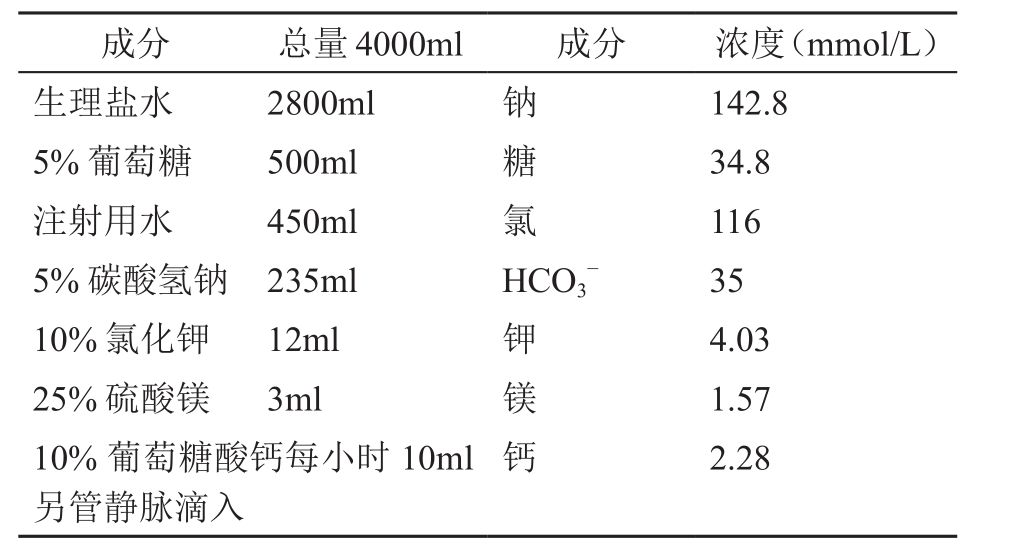
\includegraphics[width=3.36458in,height=1.84375in]{./images/Image00528.jpg}
\end{table}

附:置换液离子浓度计算公式:

Na\textsuperscript{+} 浓度(mmol/L)={[}0.9\%氯化钠(L)× 154 +
5\%碳酸氢钠(L)× 595{]}/总体积(L)

HCO\textsubscript{3} \textsuperscript{−} 浓度(mmol/L)=
5\%碳酸氢钠(L)× 595/总体积(L)

K\textsuperscript{+} 浓度(mmol/L)= 10\%氯化钾(ml)× 1.342/总体积(L)

葡萄糖浓度(mmol/L)= 5\%葡萄糖(L)+ 277.8/总体积(L)

在此标准配方中,液体的总量是4L,可以使用市场上销售的3L装的生理盐水为基础进行配制,因此,配制方法较为方便。另外,配方中的钙液另路输入,避免和碳酸氢盐混合,产生沉淀。

在治疗过程中,需要根据监测患者血中电解质及酸碱,对置换液电解质和酸碱进行调整,笔者体会到,这个过程中容易发生计算错误。为简化计算,减少错误的发生,在标准配方的基础上现将常用的调整配方列表排出,以供查阅(表\ref{tab143-2}~表\ref{tab143-4})。

\begin{table}[htbp]
\centering
\caption{钠浓度调整}
\label{tab143-2}
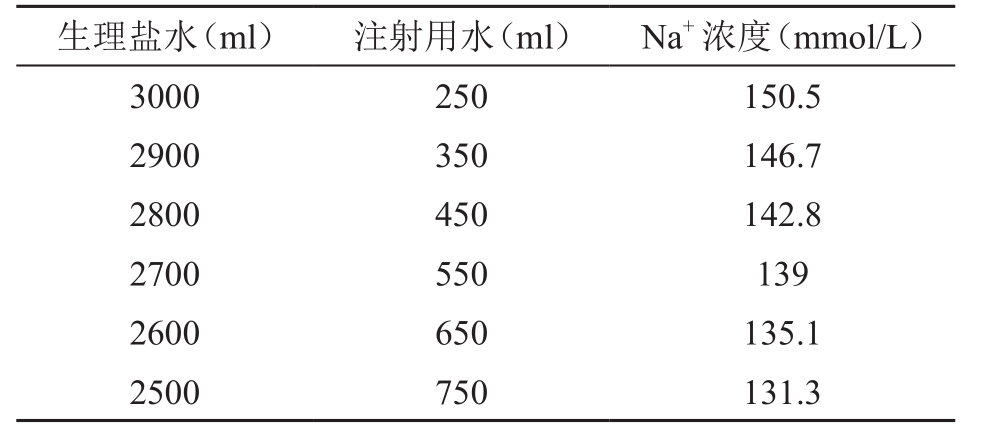
\includegraphics[width=3.3125in,height=1.42708in]{./images/Image00529.jpg}
\end{table}

\begin{table}[htbp]
\centering
\caption{{} 浓度调整}
\label{tab143-3}
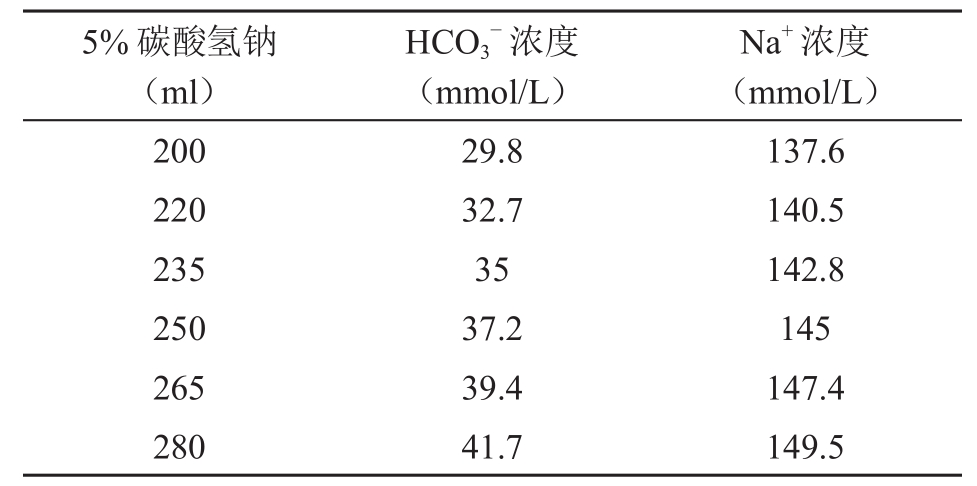
\includegraphics[width=3.25in,height=1.60417in]{./images/Image00531.jpg}
\end{table}

\begin{table}[htbp]
\centering
\caption{钾浓度调整}
\label{tab143-4}
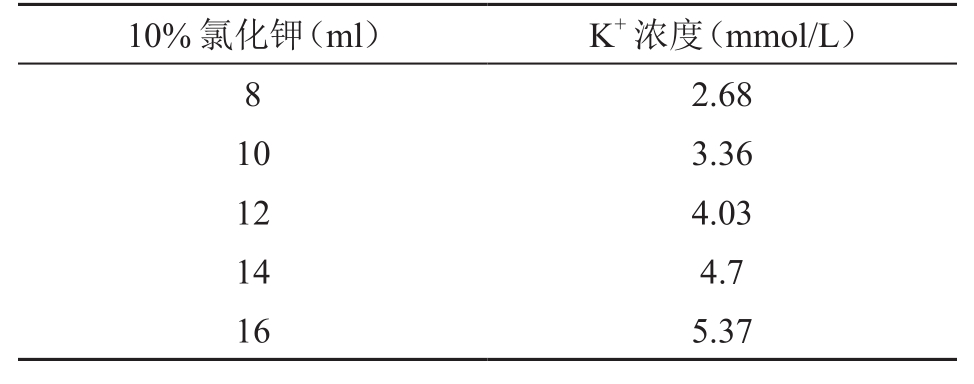
\includegraphics[width=3.23958in,height=1.27083in]{./images/Image00532.jpg}
\end{table}

\hypertarget{text00391.htmlux5cux23CHP16-10-2-3-6}{}
(六) 抗凝剂的应用

持续性血液净化治疗需要应用抗凝剂,以保证滤器的有效性。但危重患者常并有较严重的出凝血功能障碍,尤其是大手术后患者及有活动性出血的患者,抗凝剂的应用有很大风险。目前虽有多种抗凝剂及抗凝方案选择,但抗凝方案均应个体化。抗凝方案应尽量减轻血滤器的膜和血路对凝血系统的激活作用,同时可长时间维持血滤器和血路的有效性;尽量减少全身出血的发生率,将抗凝作用局限在体外循环的血滤器和血路内。和传统血液净化不同,持续性血液净化的时间长,抗凝剂使用的量相对要大些,加上患者的全身情况复杂,大多数患者都有出血倾向或已有出血发生。因此,如何保证净化治疗能顺利进行,而又不引起出血或加重出血并发症,这是在持续性血液净化治疗过程中需要时刻都要考虑的问题。

\subparagraph{普通肝素}

是目前在血液净化中最常用的抗凝剂。普通肝素是硫酸多聚糖的异质复合物,分子量在5~30kD,它是通过与循环中的抗凝血酶结合介导的。因此肝素的抗凝作用受到抗凝血酶-Ⅲ(AT-Ⅲ)的影响。危重患者的AT-Ⅲ浓度通常是下降的,这会影响肝素的活性。AT-Ⅲ下降的原因通常是因凝血酶系统激活消耗过多和因肝功能下降合成减少所致。其他影响因素包括患者的体重和凝血功能状况。肝素的作用能被鱼精蛋白中和。

持续性血液净化肝素使用方法:①首先将肝素注入盐水中,对管道和滤器进行处理;②治疗开始后,定时从血路中注入肝素。在3000ml盐水中加入12
500u的肝素对管道和滤器进行预冲,治疗开始,即从血路中注入首剂肝素1250~2500u,随后,每小时注入250~500u的肝素,根据监测的结果对肝素的用量进行调节。

治疗过程中需要监测:①部分凝血酶原时间(APTT),使其保持在正常值的1~1.5倍;②通过机器的监测系统,观察管路和滤器的各项压力指标,可以及早发现管路和滤器是否有堵塞的倾向;③监测滤器的滤过效率,可以把尿素氮作为指标,定时比较血液和滤过液中的浓度,如滤过率下降,意味着滤器的效率下降,提示抗凝不充分。

在使用肝素抗凝时,应注意个体化原则,要仔细观察,尽早摸索出患者的适宜剂量,并根据监测的结果和治疗的需要对肝素的用量进行调整。

\subparagraph{低分子肝素}

普通肝素可以数种方式裂解为较短的多糖------低分子肝素。低分子肝素有显著不同的药理特点。其分子量为4~6.5kDa,它抑制因子Xa的作用是抑制凝血酶作用的2~4倍。与普通肝素相比,低分子肝素更能预测剂量-效应关系,半衰期较长,对血小板功能影响较小。鱼精蛋白对其不起作用。低分子肝素目前也常用于持续性血液净化的抗凝。首剂从血路注入3000U,以后每4小时注入1000~2000U,根据监测的结果和治疗的需要进行调整。

\subparagraph{局部肝素抗凝}

这种抗凝方法是利用鱼精蛋白能中和肝素的抗凝活性,从而消除肝素的全身作用,减少肝素所引起的并发症。具体的做法是,将肝素在滤器前的血路注入,防止体外的血路产生凝血,在滤器后的血路注入鱼精蛋白,消除肝素的作用。

关于肝素和鱼精蛋白剂量比例关系,目前大多认为,1000U肝素对10mg鱼精蛋白,需要考虑到肝素的半衰期,肝素用量越大,半衰期越长,因此,要根据监测的结果对肝素和鱼精蛋白的用量进行调整。

\subparagraph{局部枸橼酸盐抗凝}

在滤器前的血路中注入枸橼酸盐,它们结合血中的离子钙,起到抗凝作用,然后在滤器后的血路中注入氯化钙,以补充血中的离子钙,这就是局部枸橼酸盐抗凝。局部枸橼酸盐抗凝主要用于有高度出血倾向的患者。对于有高度出血倾向的患者,有时可应用无肝素血液净化,但对血流量的要求较高。局部枸橼酸盐抗凝对血流量要求不高,引起代谢性碱中毒的可能,应引起注意。

\hypertarget{text00391.htmlux5cux23CHP16-10-2-3-7}{}
(七) 治疗过程中的监测

\subparagraph{血流动力学监测}

在治疗开始的阶段,要特别注意监测患者的血流动力学。从体内引血出来,对血流动力学会产生较大的影响,对于危重患者更是如此。如患者血压偏低,最初的血流量不妨小些,待血压稳定后再逐步增加血流量。在进入持续治疗的状态后,净化治疗对血流动力学影响变小,血压、心率会相对稳定。此时如出现血压、心率的变化,要考虑是病情本身的变化所致。

\subparagraph{电解质、酸碱平衡的监测}

持续性血液净化治疗时间长,治疗剂量大,容易发生电解质、酸碱紊乱,需密切监测,并根据监测结果调节置换液的配方。一般在治疗初期发生紊乱的概率大些,要特别注意。

\subparagraph{凝血功能监测}

应用抗凝剂是持续性血液净化所必须,使用剂量的大小应遵循个体化原则。剂量太大会导致出血,太小则引起滤器的堵塞。因此,必须监测凝血功能,并据此来调节剂量。另外,通过监测滤器的跨膜压,来调节抗凝剂的用量。如跨膜压在短时间内快速升高,提示滤器内有凝血,需要加大抗凝剂的用量。

\subsubsection{持续性血液净化的缺点}

\subparagraph{工作量明显增多}

治疗期间,需要监测,包括对患者和机器,增加很多工作量。

\subparagraph{患者需要制动}

患者长时间的制动会带来一定的并发症,如血栓形成、皮肤损害等,对于神志清醒的患者,较难配合接受长时间的制动。

\subparagraph{费用高}

从目前的收费情况来看,持续性血液净化一天的收费是一次传统血液净化收费的4~6倍,费用高的原因在治疗时间长和消耗多,这也限制了该项技术的更广泛应用。

持续性血液净化是近年来发展的新技术,和传统的血液净化相比,它有诸多的优点,但也有局限性,不能完全替代传统的血液净化。要充分考虑它的特点,根据患者的具体情况加以选择,做到物尽其用。

\protect\hypertarget{text00392.html}{}{}

\section{血液灌流在急危重症中的应用}

血液灌流是将患者血液引入灌流器,通过灌流器中吸附剂或其他生物材料的作用,清除体内有害的代谢产物或外源性毒物,经过净化后的血液返回体内的一种治疗方式。血液灌流的吸附剂常为活性炭或树脂。不同的吸附剂对每种毒素的亲和力不同,其吸附的范围也不同。目前血液灌流多用于药物过量或中毒、肝昏迷、免疫系统疾病等的治疗。血液灌流常和血液滤过结合起来,能更好地清除体内的毒性物质,这一治疗形式在肝功能不全的患者中有重要的地位。

\subparagraph{适应证}

①各种药物、毒物中毒;②急、慢性肾衰竭;③重症肝炎、肝性脑病;④流行性出血热;⑤高脂血症;⑥脓毒症;⑦全身炎症反应综合征;⑧重症感染;⑨免疫性疾病;⑩其他疾病:精神分裂症、甲状腺危象等。

\subparagraph{临床应用技术方法}

(1) 建立静脉通道:同血透。

(2)
肝素化:因为吸附剂表面较透析膜粗糙且表面积较大,肝素用量较大。采用全身肝素化的方法,首次剂量按1.0~2.0mg/kg体重,最大剂量2.5mg/kg体重,静脉给肝素10分钟后,才能开始血液灌流系统的体外循环,灌流开始20分钟时,一次追加肝素5~8mg,以后每半小时一次追加肝素5~8mg。因个体对肝素的敏感性及肝素的效价差异较大,为了不发生凝血,最好根据APTT调节肝素用量,使APTT保持在45~60秒。患者如有出血倾向,灌流结束时用鱼精蛋白中和肝素,用量与肝素之比为1∶1,使凝血时间正常化。

(3)
血液灌流装置:由灌流罐、吸附剂、微囊膜组成。目前用于临床的主要有白蛋白火棉胶包裹活性炭、丙烯酸水凝胶包裹活性炭和醋酸纤维包裹活性炭等。活性炭通常是8~14目的椰壳炭。

(4)
血流量一般在100~200ml/min左右。流速越慢,吸附率越高,所需灌流时间越短,但凝血机会相对增加,应适当提高肝素用量;反之,流速越快,吸附率越低,所需灌流时间越长。

(5)
灌流持续时间一般以2小时为宜,此时吸附剂表面已接近饱和,吸附率明显下降,血浆清除率显著降低。若有必要并允许可更换一只灌流器继续灌流,或数小时后再进行灌流。

\subparagraph{血液灌流治疗过程中的监测}

同血透。

\subparagraph{血液灌流的并发症}

同血透。

\protect\hypertarget{text00393.html}{}{}

\section{血浆置换在急危重症中的应用}

血浆置换是指将患者血液引出,用血浆分离器将血细胞与血浆分离,去除血浆以清除患者血浆中抗体、免疫复合物及毒素等物质,然后补充等量的新鲜冷冻血浆或人血白蛋白等置换液,从而达到治疗目的的一种血液净化方法。血浆置换治疗疾病的主要机制在于清除体内的致病因子,包括内源性致病因子和外源性致病因子,而这些致病因子存在于血浆中,以大分子的形式存在或和血液蛋白结合,既不能有效地用药物抑制和排出,也不能使用血液透析加以清除。主要用于治疗自身免疫性疾病、肝功能衰竭、血液病及甲状腺危象等疾病。

\subsubsection{适应证}

\subparagraph{各种原因引起的中毒}

毒蕈碱中毒、毒蘑菇中毒、有机磷农药中毒、急性药物中毒、毒鼠强中毒、急性重金属中毒(如砷化氢中毒)、毒蛇咬伤中毒以及食物中毒等,尤其是与蛋白质、血脂结合的毒素,效果更佳。

\subparagraph{肾脏疾病}

肺出血肾炎综合征、狼疮性肾炎、紫癜性肾炎、IgA肾病、膜增殖性肾炎及移植肾的急性排斥反应。

\subparagraph{自身免疫性疾病}

系统性红斑狼疮、结节性多动脉炎、皮肌炎、类风湿关节炎、大疱性皮肤病、天疱疮、类天疱疮、中毒性表皮坏死松解症、坏疽性脓皮病等。

\subparagraph{血液系统疾病}

自身免疫性溶血性贫血、溶血性尿毒症综合征、血栓性血小板减少性紫癜、高黏血综合征。

\subparagraph{神经系统疾病}

如重症肌无力、多发性神经根炎、系统性红斑狼疮的神经系统损害和多发性硬化。

\subparagraph{急 、慢性肝功能衰竭}

如暴发性病毒性肝炎、药物中毒性肝损害、肝昏迷、胆汁淤积性肝病、高胆红素血症等。

\subparagraph{器官移植}

器官移植前去除抗体(ABO血型不兼容移植、免疫高致敏受者移植等)、器官移植后排斥反应。

\subparagraph{其他}

家族性高胆固醇血症、甲状腺危象等。

\subsubsection{禁忌证}

无绝对禁忌证,相对禁忌证包括:①对血浆、人血白蛋白、肝素等有严重过敏史;②药物难以纠正的全身循环衰竭,低血压;③非稳定期的心、脑梗死;④颅内出血或重度脑水肿伴有脑疝;⑤存在精神障碍而不能很好配合治疗者。

\subsubsection{临床应用技术方法}

1.建立静脉通道 同血透。

2.确定治疗处方
①血浆置换频度:取决于原发病、病情的严重程度、治疗效果及所清除致病因子的分子量和血浆中的浓度,应个体化制订治疗方案,一般血浆置换疗法的频度是间隔1~2天,一般5~7次为1个疗程。②血浆置换剂量:单次置换剂量以患者血浆容量的1~1.5倍为宜,不建议超过2倍。患者的血浆容量可以按照下述公式进行估算:PV
=(1 − HCT)×{[}b +(c × W){]}

其中:PV:血浆容量的单位为ml,HCT:血细胞比容,W:体重的单位为kg。b值:男性为1530,女性为864;c值:男性为41,女性为47.2。

3.抗凝剂的应用
①全身肝素化法,为常规方法。治疗前5分钟,给肝素0.5~0.8mg/kg,静注治疗开始后每小时追加肝素10mg;治疗结束前1小时停用肝素。②低分子肝素一般选择60~80IU/kg,推荐在治疗前20~30分钟静脉注射,无需追加剂量。③出血风险高的患者,在监测APTT下调整。

4.置换液的种类
①晶体液:生理盐水、葡萄糖生理盐水、林格液,用于补充血浆中各种电解质的丢失。晶体液的补充一般为丢失血浆的1/3~1/2,大约为500~1000ml。②血浆制品:新鲜血浆、新鲜冰冻血浆、纯化的血浆蛋白,因其含有大部分的凝血因子、白蛋白和免疫球蛋白,对于存在凝血因子缺乏或其他因子缺乏的患者,可考虑使用。③人白蛋白制剂:常用浓度为4\%~5\%。④血浆代用品:主要有中分子右旋糖酐、低分子右旋糖酐、羟乙基淀粉等,但在体内的半衰期只有数小时,故总量不能超过总置换量的20\%,并应在治疗起始阶段使用。血浆代用品可以降低全血黏度,改善微循环,适用于骨髓瘤和巨球蛋白血症等引起的高黏滞血症。

5.血流量一般在100~150ml/min左右。血流速与血浆分离速度呈正比。跨膜压控制在6.7kPa(50mmHg)左右,血浆分离速度与跨膜压呈直线相关。

\subsubsection{血浆置换治疗过程中的监测}

同血透。

\subsubsection{血浆置换的并发症}

\subparagraph{过敏和变态反应}

系大量输入异体血浆有关,表现为皮疹、皮肤瘙痒、畏寒、高热,严重者甚至出现过敏性休克。可在血浆输入前适量应用糖皮质激素预防;出现过敏和变态反应时减慢或停止置换,停止输入可疑血浆或血浆制品,予以糖皮质激素、抗组胺类药物治疗,出现过敏性休克的按休克处理。

\subparagraph{低血压}

与置换液补充量不足、血管活性药物清除或过敏反应有关,根据不同的原因进行相应处理。

\subparagraph{溶血}

查明原因,予以治疗,特别注意所输入血浆的血型,停止输注可疑血浆;应严密监测血钾,避免发生高血钾等。

\subparagraph{感染}

在大量使用白蛋白置换液进行血浆置换时,体内免疫球蛋白和补体成分丢失。高危患者可适量补充新鲜血浆或静脉注射大剂量免疫球蛋白。

\subparagraph{血道传播病毒感染}

主要与输入血浆有关,患者有感染肝炎病毒和人免疫缺陷病毒的潜在危险。

\subparagraph{出血倾向}

与血浆置换过程中血小板破坏、抗凝药物过量、凝血因子丢失有关。对于高危患者及短期内多次、大量置换者,可补充适量新鲜血浆。

\protect\hypertarget{text00394.html}{}{}

\hypertarget{text00394.htmlux5cux23CHP16-10-5}{}
参 考 文 献

1. 朱大年.生理学.第7版.北京:人民卫生出版社,2008

2. 何志捷,管向东.重症医学.北京:人民卫生出版社,2009

3. 金惠铭,王建枝.病理生理学.第7版.北京:人民卫生出版社,2005

4. 陈文彬,潘祥林.诊断学.第7版.北京:人民卫生出版社,

2005

5. WaikarSS,Liu KD,Chertow GM. Diagnosis,Epidemiology and Outcomes of
Acute Kidney Injury. Clin J Am Soc Nephrol,2008,3:844-861

6. 中华医学会重症医学分会.ICU中血液净化的应用指南.

2010

7. van der Voort PH,Gerritsen RT,Kuiper MA,et al. Filter run time in
CVVH:pre- versus post-dilution and nadroparin versus regional
heparin-protamine anticoagulation. Blood Purif,2005,23(3):175-180

8. Uchino S,Fealy N,Baldwin I,et al. Pre-dilution vs. postdilution
during continuous veno-venous hemofiltration:impact on filter life and
azotemic control. Nephron Clin Pract,2003,94(4):c94-98

9. de Pont AC,Bouman CS,Bakhtiari K,et al. Predilution versus
postdilution during continuous venovenous hemofiltration:a comparison
of circuit thrombogenesis. Asaio J. Jul-Aug,2006,52(4):416-422

\protect\hypertarget{text00395.html}{}{}

\chapter{高压氧疗法}

\subsubsection{高压氧的基本原理}

在高压(超过常压)的环境下,呼吸纯氧或高浓度氧以治疗缺血缺氧性疾病和相关疾患的方法,即高压氧治疗。它是一种特殊的氧治疗方法,具备常压环境下一般氧疗所远不能起到的治疗作用。在治疗机制、治疗方法和治疗效果等方面较之一般氧疗都发生了极大的变化,质的飞跃。高压氧具有独特的治疗机制。

高压氧能极大的增加肺泡氧分压,提高血氧张力,增加血氧含量。在通常情况下,即常压(1ATA),血液输送氧有两种方式,一是血红蛋白结合氧(HbO\textsubscript{2}
),每克Hb可结合氧1.34ml,如一般正常人Hb含量为140g/L,Hb的氧饱和度为97\%,那么100ml血结合氧为18.2容积\%;二是血浆中的物理性溶解氧,100ml血中约为0.3容积\%,故总共为18.5容积\%,其中溶解氧占量甚微。然而在氧的传递过程中,溶解氧是非常重要的。因为不论在常压或高压下氧均以溶解状态供组织利用。在高压氧下,Hb结合氧的增加是有限的,而根据气体物理学的Dolton定律和Henry定律,血浆中的物理性溶解氧则可随氧压的增高而成正比地上升。Dolton定律(气体分压定律)指出:当温度不变,混合气体的总压力等于各组成气体分压的和;Henry定律(气体溶解定律)指出:在相同温度下,气体溶入液体的量与该气体的压强成正比。在空气成分中,氧约占21\%,氮约占78\%,CO\textsubscript{2}
约占0.04\%及其他一些稀有气体。因此,在常压正常生理情况下,呼吸空气时PaO\textsubscript{2}
在100mmHg左右,若改吸纯氧,则PaO\textsubscript{2}
可在650mmHg;氧可提高6倍以上,达2.0容积\%;当呼吸3ATA纯氧时,PaO\textsubscript{2}
可高达2140mmHg,血浆物理性溶解氧可增至6.4容积\%(此值已高于正常静息状态下一般动静脉氧含量差5.6容积\%),与常压下呼吸空气时的溶解氧0.3容积\%相比,则超过其20余倍(表\ref{tab144-1})。\footnote{此表按T 37℃ Hb 140g/L,静息状态计算;氧分压单位为mmHg}

相应地,高压氧下的淋巴液、组织间液、脑脊液、各类组织细胞的氧分压也都增高,例如,淋巴液氧分压提高10倍,约600mmHg。

高压氧能显著地增加组织的氧储量,在常温、常压下,平均每千克组织的氧储量约为13ml,正常时平均每千克组织的耗氧量为3~4ml/min,按推算,循环阻断的安全时限为3~4分钟,在3ATA下呼吸纯氧,平均每千克组织的氧储量增至53ml,相当于常压条件下的4倍多,此时循环阻断的安全时限可延长到8~12分钟;若应用氧和2\%
CO\textsubscript{2}
混合气呼吸,循环阻断的安全时间将更长,达17~26分钟;若结合低温,如从37℃降至32℃,血中物理性溶解氧增加10\%,心肌耗氧量降低20\%,脑的耗氧量降低35\%以上,使循环阻断的安全时限进一步延长;如3ATA纯氧,降温5℃,阻断循环的安全时限可达27~30分钟。

血氧分压的增加,有利于氧的弥散,压差愈大,弥散速率愈快,有效弥散半径延伸,弥散轮、弥散范围都扩大(图\ref{fig144-1})。高压氧可有效地应用于治疗因组织水肿而使毛细血管与周围细胞间距扩大的病理状态,如脑水肿、肺水肿及其他间质水肿等所造成的氧弥散障碍,也可用于毛细血管损伤或血流淤滞而造成的供氧障碍疾患,如脑梗死、小面积心肌梗死、断肢(指)再植、植皮、烧伤、冻伤、顽固性溃疡等;一般在常压下吸氧是不能足够地增加氧的有效弥散距离,而应用高压氧能达到这一目的。

\begin{table}[htbp]
\centering
\caption{高压氧下动脉血氧分压和血氧含量的变化(理论值)}
\label{tab144-1}
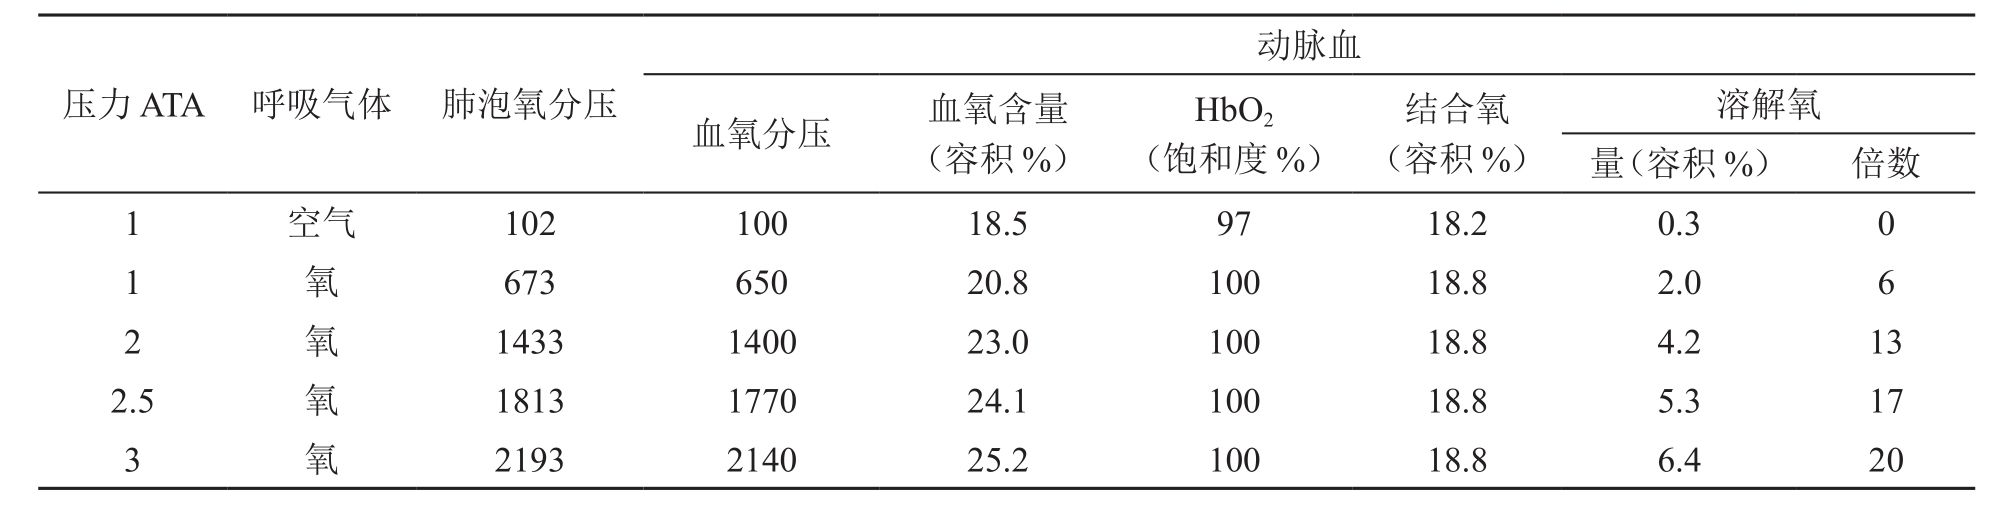
\includegraphics[width=6.67708in,height=1.67708in]{./images/Image00533.jpg}
\end{table}


高压氧能极其有效地改善机体的缺氧状态,对心、脑、肝、肾等重要器官有保护作用;高压氧有直接或反射性地引起血管收缩的作用,使血管阻力增加,血流量减少,但由于血氧含量的急剧上升,总的供氧仍有显著增加,因此既改善脑缺氧,又降低颅内压,减轻脑水肿,能有效地打断缺氧-水肿的恶性循环。因此,高压氧对组织缺氧,尤其是对脑缺氧、脑水肿、肺水肿等的治疗具有相当的价值。

\begin{figure}[!htbp]
 \centering
 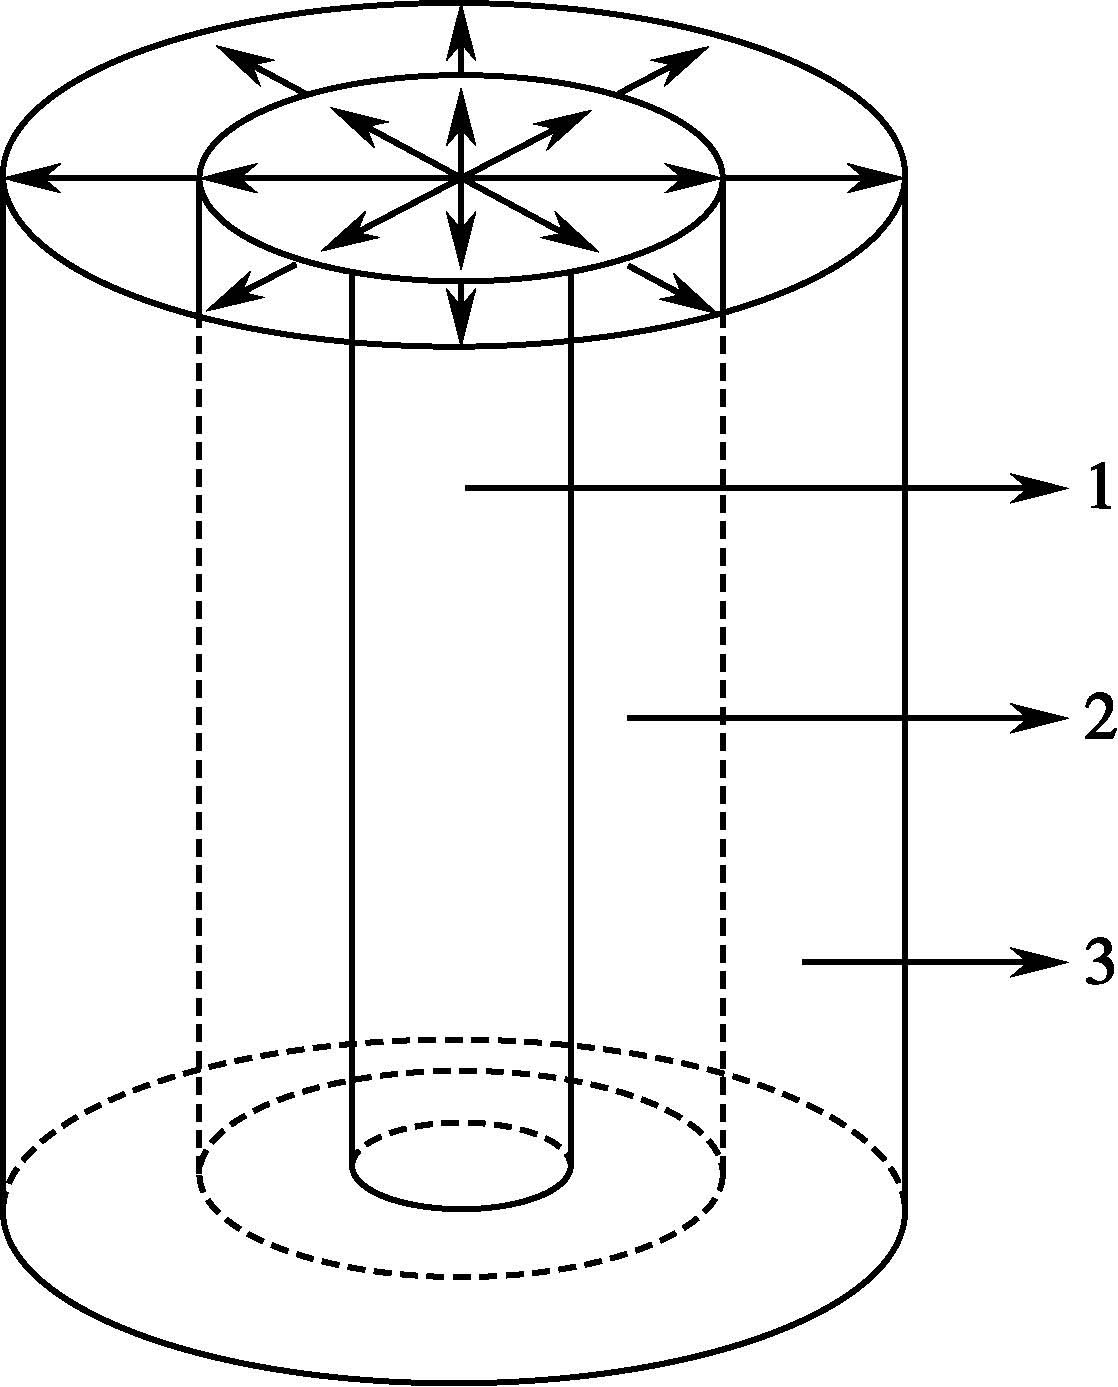
\includegraphics[width=1.85417in,height=2.3125in]{./images/Image00534.jpg}
 \captionsetup{justification=centering}
 \caption{氧在组织中的弥散(示意图)}
 \label{fig144-1}
  \end{figure} 

1.毛细血管;2.常压吸空气的弥散半径;3.高压氧的弥散半径

高压氧具有促进血管新生,创伤修复的作用。高压氧可使缺血缺氧病损区域获得有治疗意义的氧水平,达到并超过血管修复、创伤愈合所需要的临界氧张力。研究表明,成纤维细胞的移动距离决定于相邻毛细血管内及细胞外液的氧分压,成纤维细胞的分裂和产生胶原,要求至少PO\textsubscript{2}
为20~30mmHg,吸常压氧不能使病变组织局部的PO\textsubscript{2}
有效地提高,而2~2.5ATA氧可提高创伤部位的PO\textsubscript{2}
到正常水平30mmHg以上乃至更高的水平。在这种高压氧合作用下,组织细胞代谢旺盛,ATP生成增多,促进成纤维细胞的活动和分裂,以及胶原纤维的形成。从而促进血管内皮细胞的再生和新的毛细血管生成和连接,加速侧支循环的形成,Boerema曾观察到外伤性血运障碍的年轻患者,在高压氧治疗期间,侧支循环可在1周内建立。由于重建血管床,改善微循环,进一步改善了组织的缺血缺氧或低氧状态,有利于创伤组织的修复。此外,高压氧条件下,破骨细胞的活性达100\%,有利于骨再生。

高压氧有抑制和杀灭细菌的作用,尤其是对厌氧菌,并能抑制和破坏厌氧菌产生的多种毒素,如α-外毒素,能迅速有效地解除中毒症状;对需氧菌方面,高压氧可抑制其生长,如在1.3ATA氧下,葡萄球菌的生长能被抑制。此外,在创伤感染情况下,氧分压在30mmHg以下,则白细胞杀灭金黄色葡萄球菌的能力下降;应用高压氧能增强白细胞的活力和吞噬功能。因此,可以说高压氧有抗感染作用,并和某些抗生素有协同作用。

高压氧是潜水减压病和其他原因造成的气体栓塞的主要而具有针对性的疗法。气体物理学的Boyle-Mariotle定律指出:在温度、质量相同的情况下,气体的体积和压力成反比。由此气泡能因加压而缩小,重新溶解于血液;并由于吸入高压氧,取代和置换气栓的主要成分---中性气体氮,从而达到消除气泡、置换氮体,改善缺氧、逆转组织变性的治疗目的。

高压氧是最有效的放射增敏剂,可应用于配合放射线、化学药物、激光等治疗癌肿。

高压氧还被有效地应用于晚发放射损伤,是放射性组织坏死的主要治疗手段。

\subsubsection{医用高压氧舱的种类和特点}

高压氧治疗需要一个特殊的专用设备,即高压氧舱(简称氧舱)。其主体为耐压而密闭的舱体,氧舱整体系一个系统工程,其结构有加压供气系统、供氧系统、仪表控制系统、通讯照明系统、安全报警和监视系统、空调系统、生物电测试和监护系统等。现代化氧舱是一个安全、实用、简洁、舒适、美观的医疗设备。根据其规模和使用情况一般可分为以下几种类型:

\subparagraph{大型复式高压氧舱}

即三舱七门式大型高压氧舱,或大型高压氧舱群。有手术舱、治疗舱、过渡舱组成。手术舱即高压氧手术治疗室,可以从实地进行心胸外科等大型手术,定员可达20人左右;治疗舱定员可容10~16人,或更大规模。手术舱和治疗舱均可用于对危急重症病员的综合抢救治疗。手术舱和治疗舱的设计压力通常为4.2ATA,过渡舱设计压力可达7~8ATA,除供人员进出高压环境的过渡使用外,可用于潜水减压病的治疗需要。三舱之间由通道连接,可呈一列式排列,但多以直角式(L形)布局。

\subparagraph{中型高压氧舱}

通常又称多人舱,其形式和规模较为多样,如规模较大的可分两舱两室四门式,一舱两室三门式,定员可在16~20人;规模中等的如一舱两室两门式,定员8~12人;规模较小的一舱一室一门式,定员4~16人。这类舱可供多人同时治疗,医护人员陪舱直接对重危患者进行综合抢救治疗。其造价低于大型舱群,便于建造、购置、较易普及。

\subparagraph{单人舱}

通常为单人纯氧舱(舱容较大者,应急时可容两人),既可直接使用高压氧加压的小型舱,也有用压缩空气加压、面罩吸氧的类型。单人纯氧舱有很好的实用性。它可满足除高压氧下的手术和综合抢救之外的各种高压氧治疗需要,很适合于各种创伤疾患的治疗,如断肢(指、趾)再植、烧伤、植皮、难治性溃疡、压疮、血管栓塞等,特别适用于气性坏疽等特异感染的抢救治疗,便于消毒隔离,预防交叉感染。便于治疗方案设计时个别对待,区别施治。用纯氧直接加压,与用空气加压的多人舱相比,病员反映舒适感好。其特点还有机动灵活,便于运输,价值便宜,很易普及。

婴儿高压氧舱,为透明有机玻璃舱,直径为50cm,长度100cm,设计压力为2ATA,实际上就是缩小了的小型单人纯氧舱,可专用于新生儿、婴幼儿的缺血缺氧性疾患的治疗。

单人纯氧舱除有钢材制作的外,在美、英等国已普遍采用舱体为耐压的优质有机玻璃制作,如美国的Sechrist
Monoplace Hyperbaric
Systems,患者在舱内情况一目了然,除有心电监护外,还有辅助呼吸装置和加压输液装置,这样就较为理想地具备综合抢救治疗的性能。

我国对医用高压氧舱的生产管理已进入规范化、科学化、法制化的轨道,制订了GB12130~95新国标;必须经国家质量技术监督部门审定和批准,有关厂家才能生产医用高压氧舱。医疗单位应依据医院规模的大小,医疗、科研、教学等方面的需要和社会需求,从实际出发和前瞻性的考虑来配备和设置高压氧舱。

\subsubsection{高压氧治疗的治疗方法}

正确地掌握和实施治疗方法是高压氧治疗取得疗效的关键。既要周详地制订治疗方案,又要注意认真做好每一个舱次的治疗。

一次高压氧治疗包含加压、稳压吸氧、减压三个相关阶段,必须认真掌握好治疗的全过程,在各个阶段中都要牢记高压氧治疗的注意事项,必须缜密地防止可能发生的副作用和杜绝意外事故,确保安全而有效的治疗。

\subparagraph{治疗压力的选择}

高压氧舱治疗使用的压力通常分别为1.6ATA、1.7ATA、2ATA、2.5ATA、2.8ATA、3ATA等。1.6ATA用于婴幼儿的高压氧治疗、1.7ATA较少使用,或用于合并有老年性慢性支气管炎、轻度或中度肺气肿的患者。在通常的治疗中常用2~2.5ATA,急诊外科方面常用2.5ATA,并往往在初始治疗的若干次中,常用这一压力范围;尤其像对心肺脑复苏、休克、严重创伤等的高压氧治疗,其治疗压力的选择,应以既能迅速产生“高氧效应”、减轻组织水肿等为出发点,又不能因过高压力环境给机体带来超负荷的影响,应用足够而又适当的压力,起初2~3天使用压力可为2.5ATA,然后维持治疗时可用2ATA
或2.2ATA,以获得或超过组织修复所需要的临界氧分压;对严重创伤,包括并发创伤性休克等,都采用2.5ATA,并以此维持治疗为佳;对失血性休克,为代偿血容量可用2.5ATA、2.8ATA乃至3ATA;对晚期气性坏疽则用3ATA,以迅速有效地抑制和杀灭厌氧菌,并破坏其毒素的产生。治疗气栓症使用3ATA,主要是依据Bolye定律所揭示的原理,来选择治疗压力范围。

\subparagraph{吸氧方案}

采用间歇吸氧方式,按照压力-吸氧时限来界定。Lambertsem报告2ATA吸氧2.5小时,肺活量减少2\%,若间歇5~10分钟,则可延长吸氧时间,保护肺组织,可以大大提高安全度,防止肺氧中毒;3ATA吸氧必须警惕神经型氧中毒的发生。具体吸氧方案一般有以下几种,如2ATA
20分钟× 4(间歇5分钟);30~40分钟× 2(间歇5~10分钟);2.5ATA 20分钟×
4(间歇5分钟),30~40分钟× 2(间歇5~10分钟);3ATA 20~30分钟×
2(间歇5~10分钟)。对急诊外科等危急重症的高压氧治疗,宜采用2~2.5ATA
40分钟× 2或30分钟×
3(间歇5分钟)的稳压吸氧方案,并且加减压阶段均吸氧,即除间歇时间外,加减压及稳压阶段全过程吸氧,并必须采用一级供氧方式。

单人纯氧舱的吸氧方案:2ATA 120分钟,2.5ATA 100分钟,3ATA
40~60分钟。婴儿舱为1.6ATA 60分钟。

\subparagraph{减压方案}

高压氧治疗有多种减压方案,如均匀等速减压和阶梯式减压法等。但对危急重症病例均宜采用缓慢、等速、吸氧减压法,直至减压出舱后仍继续吸氧,以使机体适应从高压氧环境到常压环境的平稳过渡。对脑缺氧脑水肿患者也是预防脑压“反跳”的有效措施之一。

\subparagraph{疗程安排}

高压氧治疗通常都不是一两次治疗就告完成的,而是要数次,数十次,即几个疗程乃至相当长期的多个疗程治疗,以期取得最佳的疗效。通常人为地拟订10~12次为一个疗程。例如,对一般创伤病患,为逆转创伤局部缺氧变性,促使组织存活,或对具有特殊疗效的气性坏疽、气栓症等高压氧治疗1周或1个疗程(相当于7~10次),即见分晓;而对于重型颅脑损伤、脊髓损伤、长期昏迷、PVS及严重的神经系统后遗损害等,则需用40~60次(4~6个疗程)以上,乃至更长疗程的高压氧治疗。总体说来,其疗程的安排是根据疾病种类、病情变化、机体的功能状态、年龄等因人而异;对一些常见的治疗适应证可有一定的治疗模式,但不能千篇一律地机械式地套用;对于急诊医学等方面危急重症的高压氧抢救治疗,必须认真掌握早期治疗、综合治疗、长疗程治疗,高气压条件下安全和合理用氧,防止副作用和并发症,以及区别施治等治疗原则,全面考虑、精心设计治疗方案,科学地制订和安排疗程。

\subsubsection{高压氧治疗的适应范围和禁忌证}

\subparagraph{适应范围}

在高压氧成功地应用于阻断循环心内直视手术等的同时,并确立了CO中毒、潜水减压病、气性坏疽等为高压氧治疗的绝对适应证,随着研究和临床实践的不断深入,高压氧治疗已涉及内、外、妇、儿、眼、五官、皮肤等临床各科,约160余个病种。其适应范围概括地说:即各种原因所致的全身或局部缺血缺氧性疾患及其有关病损。在急诊外科疾患方面,如休克、外伤性心搏呼吸骤停、颅脑损伤、脊髓损伤、挤压综合征、断肢再植、烧伤、加速创面愈合和提高植皮存活率、外科感染如厌氧菌感染等,高压氧治疗已被广泛采用。

\subparagraph{禁忌证}

未经控制的内出血(尤其是颅内出血)、癌肿(配合放疗、化疗等除外)、气胸、肺大泡、严重肺气肿、肺部感染、原因不明的高热、血压超过160/100mmHg、眼压过高、急性上呼吸道感染、急性或慢性鼻窦炎、中耳炎、精神失常等。

\subsubsection{高压氧治疗可能发生的副作用}

\subparagraph{减压病}

系由于在高压下过快减压,使溶解在血液中的氮气大量逸出,形成气泡,在血管内外形成栓塞和压迫所导致的病变。妥善地制订加压治疗方案、采用阶段减压法和按规定时间的缓慢等速减压法、吸氧减压法等可以预防。一旦发生,立即应用高压氧治疗解救。

\subparagraph{氧中毒}

在高压下吸氧或长时间吸高浓度都会发生氧的毒性作用。前者重点影响中枢神经系统和肺,后者则主要导致肺氧中毒。一般认为常压下的连续吸纯氧12~24小时以上,2ATA连续吸纯氧4~6小时以上,3ATA连续吸纯氧2小时以上,即可导致不同类型的氧中毒。氧中毒分为四个类型:神经型氧中毒、肺型氧中毒、溶血型氧中毒、眼型氧中毒。2.5ATA以上压力超过吸氧时限即可出现神经型氧中毒,3ATA连续吸氧3小时,几乎每人都将发生癫痫大发作。3ATA以上超过时限吸氧因代谢迅速紊乱,来不及表现肺部损害,而以神经型氧中毒表现为主。一般神经型氧中毒只要处理恰当,不会导致永久性损害。2~2.5ATA以下压力吸氧及常压下吸高浓度氧,易导致肺氧中毒,除与压力-吸氧时限有关,在已有肺部损害的患者,如肺部感染、肺气肿、极度衰弱者更易引起。应用高压氧抢救治疗危重病例、肺氧中毒比其他类型氧中毒多见,而神经型氧中毒可能在使用3ATA治疗气性坏疽或其他需要更高压力治疗疾病(如减压病等)时发生。此外,还有溶血型氧中毒,研究发现机体在高压氧环境中,可以发生不同程度的溶血,其程度随氧压的增高和持续时间延长而加重。但常规的高压氧治疗甚罕见,所造成的溶血也极微,无明显临床意义。眼型氧中毒,高压氧可使未成熟婴儿产生晶体后纤维组织增生、血管增生、视网膜功能障碍,因此对孕妇和6个月以内的婴儿进行高压氧治疗应当慎重。

对于氧中毒,存在着个体差异,它可通过氧敏感试验反映出来。一般认为下列压力-吸氧时限是安全的,2ATA
2小时,2.5ATA 1.5小时,3ATA
1小时。在高压氧治疗中,严格控制压力-吸氧时限,并采用间歇吸氧法,氧中毒是可以预防的。此外,巴比妥类、水合氯醛、维生素C、E等药物对氧中毒的发生有预防和保护作用。

\subparagraph{气压伤}

机体某些空腔部位,在加减压过程中,由于受压不平衡而引起相当的压差,可引起局部充血、水肿、疼痛,甚至损伤,如中耳气压伤、鼻窦气压伤、肺气压伤等。

\hypertarget{text00395.htmlux5cux23CHP16-11-5-3-1}{}
(1) 中耳气压伤:

或称气压损伤性中耳炎,是高压氧治疗中较易发生的副作用,有时可合并内耳气压伤。其病情表现取决于鼓室与外界的压差值:①10~30mmHg时,可致耳膜凹陷,鼓膜松弛部位及锤骨柄附近内层充血;②60mmHg时,耳疼痛感,中耳黏膜血管扩张,出现充血及渗出;③80~100mmHg,剧烈耳痛及放射痛,鼓膜广泛充血,听力减退,中耳腔有渗出液。压差90mmHg时,咽鼓管即不可能再张开,即是使用捏鼻鼓气法(Valsalva咽鼓管吹张法)亦不能张开;④压差为120~200mmHg时,鼓膜穿孔、破裂、剧痛可随即消失,血性渗出液从外耳道流出或流入中耳及乳突小房,而感到耳内有一股温热感。

\hypertarget{text00395.htmlux5cux23CHP16-11-5-3-2}{}
(2) 鼻窦气压伤:

在压差0.1ATA时,即可致剧痛。窦腔内的出血或血性分泌物在减压时可经鼻腔流出。

中耳气压伤、鼻窦气压伤一经发生,应及时调整加减压方案,并按对中耳炎或鼻窦炎的治疗方法对症处理。

\hypertarget{text00395.htmlux5cux23CHP16-11-5-3-3}{}
(3) 肺气压伤:

主要发生在减压过程中,是由于肺内压突然高于或低于外界压力,压差大于80mmHg导致肺组织撕裂和血管损伤,以致气泡进入血管和与肺相邻的部位,从而产生的一种紧张危险性疾患,它主要见于某些潜水事故和海滩中。高压氧治疗减压过程中,患者突然屏气或剧烈咳嗽,也有可能引起肺气压伤。有效的治疗方法是加压治疗,并对气胸等并发症紧急处理、对症治疗、积极抢救。

\subparagraph{禁闭忧虑症}

严重者为幽闭恐怖。国外有学者报道这类症象发生。笔者所在医院应用大型及小型高压氧舱治疗累计18万人次,无1例发生。主要是在进舱前对清醒患者进行详细的安全宣教和安慰,讲解注意事项,解除心理障碍。

\subsubsection{高压氧治疗的注意事项}

高压氧医学是高度重视安全的学科,在高压氧舱运行的全过程和治疗操作的每一细节,都必须强调安全第一。必须严格制订高压氧治疗各项工作规章制度,严格制度和遵守操作规程,确保治疗安全和设备安全,彻底杜绝爆燃等恶性事故。

1.严禁火种
高压氧环境兼有高压和富氧两方面的特殊因素,必须严禁火种,严禁携带易燃、易爆等危险物品进舱,舱内的装饰材料应均为不可燃性材质制成。单人纯氧舱内严防静电火花,严格着装要求,严禁穿戴化纤、尼龙类服饰,应沐浴更衣,穿着由医院专门制做的全棉衣物;女性长发加湿,清除一切化妆品和油脂类物品。

2.严格控制舱内氧浓度
控制多人舱内氧浓度在25\%以下(国外规定不超过23.5\%),严密监测并做好通风换气,可以避免在舱内发生剧烈燃烧和爆燃等恶性事故。

3.防止损伤性事故
在舱内的一切操作都必须注意压差改变带来的影响,防止造成损伤。如输液,在加减压过程中,均会影响滴液速度,应随时予以调整,尤其在减压阶段,要警惕因输液瓶内压力高于外界压力,使输液速度过快发生气栓等危险。有时可向输液瓶内插入足够长的针头(如血浆分离针)超过液平面,保证排气,使瓶内外压力平衡;又如所有引流必须通畅,并防止反流,在减压时所有皮条或引流管均应开放,防止空腔脏器或有关部位因压力膨胀、扩张而造成损伤。气管插管的导管气囊也应开放,并及时吸出分泌物,保持呼吸道通畅;再如10ml以上安瓿应在舱外开启后从递物舱递进备用等。

4.认真做好陪舱舱内的各项监护工作
实质上高压氧舱就是高压氧这个特殊环境下更高层次的ICU。在首次治疗或某次治疗中视情况必要时,在稳压吸氧结束、即将减压前做血气分析检测,对休克脑复苏病例可作为一项常规以明确供氧真实效果。抢救危重患者时要做好陪舱抢救治疗记录。

5.压氧舱必须配备急救药箱(车),便于随时急用。

6.严格执行消毒隔离制度,预防交叉感染
除做好日常性的舱体环境、呼吸器具等消毒外,在安排手术前或治疗厌氧菌感染后均必须按规定要求,彻底大扫除,严格消毒处理。

7.做好经常性的设备维护工作
按使用年限,做好设备的年检及小修、中修(3~5年)、大修(5~10年),保证设备安全运行。

8.给予医务保障
从事高压氧治疗的医务人员应是能适应高气压工作环境者,并应给予相应的保健措施和医务保障。

\protect\hypertarget{text00396.html}{}{}

\chapter{输血与输血反应}

输血(blood
transfusion)指给患者输注供者的血液成分或全血,是一种替代治疗。用以补充血容量维持有效血液循环,恢复氧、CO\textsubscript{2}
、营养、代谢产物的运输能力,保持血液免疫、抗感染、止凝血和抗凝功能。是外科手术、创伤、血液病及各种危急重症患者的重要治疗措施之一。成分输血(blood
component
therapy)是临床输血的主要形式,按照“缺什么补什么”的原则,只给患者输注需要的高浓度、高纯度、低容量血液成分,不仅可以充分利用全血,而且可以减少各种输血反应。

\section{输血与成分输血}

\subsubsection{全血}

全血,包括血液的全部成分。国内一般以200ml为1U,国际上以450ml为1U。新鲜血指当天采集或采集时间在24小时内的血液。为了防止血液凝固,延长保存时间,须在血液中加入保存液,常用的枸橼酸-枸橼酸钠-葡萄糖液(ACD液),在4~6℃温度可保存21天。保存过程中的血液成分变化如下:红细胞存活率随保存时间延长而逐渐降低(21天后仅维持70\%左右),红细胞内ATP和2,3-DPG逐渐下降,导致血红蛋白对氧的亲和力增加,因而对组织供氧减少,氧解离曲线左移;白细胞的生存时间除淋巴细胞较长外,粒细胞在周围血液内的生存期为6~8小时,很难延长保存,1天后即功能丧失;血小板易于聚集破坏,保存12小时后大部分活性减低,24小时后活性丧失;凝血因子Ⅷ在全血内保存24小时后,活性显著下降,因子V保存3~5天后也损伤50\%,纤维蛋白原、凝血酶原及其他凝血因子的活性也随保存时间延长其活性不同程度地降低;此外,保存血中电解质,如钾、氨离子、乳酸、丙酮酸含量增高,Ca\textsuperscript{2+}
降低,pH逐渐下降。

输入新鲜全血可增加有效循环血容量,改善心排血量,提高红细胞携氧能力,增加凝血因子,提高凝血功能,并能补充血浆蛋白,维持血液渗透压;血液中含有各种抗体,能改善机体的免疫功能。输全血的主要适应证是:①出血、创伤、手术、烧伤等致使血容量减少30\%以上或临床伴有休克时;②应用于体外循环及血液透析患者,最好用新鲜血(因体外循环装置能使血小板减少50\%~70\%);③有全血细胞减少如再生障碍性贫血或急性白血病等。

由于输注全血较多的不良反应,红细胞输注已逐步替代全血输注。

\subsubsection{红细胞输注}

红细胞输注(red cell
transfusion)用于:①补足血容量恢复有效的血液循环。如外伤、消化道出血等急性失血时,在积极补液的同时需输注红细胞。②纠正贫血时的缺氧状态。贫血时输血应个体化:通常无缺血危险因素,Hb水平在60~80g/L,无需预防性输注红细胞;手术患者需要输注红细胞的阈值为80g/L;老人、儿童及有心肌缺血、心肌梗死、心力衰竭、慢性肺部疾患和慢性肾病等,输血阈值为100~110g/L。常用红细胞制品有:

1.浓缩红细胞(红细胞浓缩液)
全血用沉淀法或离心法移去部分血浆而制得。每单位(袋)的总量为110~120ml,其中含有200ml全血中的全部红细胞,30ml左右血浆及15ml左右抗凝剂,血细胞比容(Hct)0.70~0.80。具有和全血同样的携氧能力,而容量仅有全血的一半,同时抗凝剂、酸、钾、氨等比全血少,适用于心、肝和肾功能不全的患者,老年、儿童患者更为安全。给体重70kg患者每输入1U可增加Hb
10g/L或Hct增加0.03。保存期较短(24小时),须及时使用。适应证:①各种贫血;②心、肾、肝功能不全需要输血者;③小儿和老年人需要输血者;④妊娠后期并发贫血需要输血者;⑤急性出血或手术失血低于1500ml的患者可在应用胶体及晶体液补足血容量的基础上输注浓缩红细胞。

2.悬浮红细胞(suspended red blood cells)
每单位含200ml全血中的血细胞和约30ml的血细胞添加剂,总量约130ml,有浓缩红细胞的优点且保存期较长(35天),血黏度低。适应证同浓缩红细胞。

3.洗涤红细胞(washed red blood
cells)用生理盐水反复洗涤浓缩红细胞,除去补体、抗体和血浆。每单位含200ml全血中的血细胞和约50ml的生理盐水,总量约120ml。本制品已去除80\%以上的白细胞和99\%的血浆,仅留下至少80\%的红细胞。在洗涤中同时去除了钾、氯、乳酸、抗凝剂和微小凝块等,血小板亦随血浆被移出去,可显著降低输血不良反应。4℃保存24小时。适应证:①有免疫因素溶血性贫血,如自身免疫性溶血性贫血和阵发性睡眠性血红蛋白尿需输血者;②新生儿溶血性贫血;③输入全血或血浆后发生过敏反应或发热者;④高钾血症及肝、肾功能障碍需要输血者;⑤由于反复输血或妊娠对白细胞、血小板产生抗体需要输血者;⑥IgA缺乏有抗IgA抗体者。依病情决定用量,估计成人患者每输注3个单位洗涤红细胞可提高Hb
10g/L或Hct增加0.03。

4.冰冻红细胞(frozen red blood cells)
由200ml全血制备,在−80℃条件下可冰冻保存10年以上。不含白细胞、血小板和血浆。适应证为:①对稀有血型的人储存红细胞;②对具有多种红细胞同种抗体的人进行自家输血;③对准备器官和骨髓移植的患者,降低组织相容性抗原的同种免疫作用。

5.辐照红细胞(irradiated red blood cells)
经25~30Gy的γ射线照射,以破坏有免疫活性淋巴细胞的有丝分裂能力,预防输血相关移植物抗宿主病的发生。供免疫缺陷患者、骨髓或器官移植后输血用。

6.少白细胞的红细胞(leukocyte-reduced red blood cells)
利用过滤法或沉淀技术将浓缩红细胞中的白细胞除去90\%以上而制得。每单位(袋)总量120ml,其中含红细胞60~80ml,生理盐水50ml。在已去除的白细胞中,粒细胞和单核细胞去除最多,淋巴细胞去除最少,输血反应少,4℃保存24小时。适应证:①发热,有严重过敏性输血反应者;②由于多次妊娠或反复输血已产生白细胞或血小板抗体引起输血反应的患者;③准备骨髓或器官移植者。

7.年轻红细胞(young red blood cells)
是用血细胞分离机制备的成熟程度在网织红细胞与成熟红细胞之间的红细胞。本制品的最大特点是含有高度的新生红细胞,这种红细胞输入人体后存活时间比普通红细胞长,携氧能力比一般红细胞强,是需要长期输血的患者最为理想的血液制品。主要用于需长期输血的患者,如重型β-地中海贫血、慢性严重的再生障碍性贫血,以便延长输血的间隔时间、减少输血次数、减少铁负荷过多的发生。

\subsubsection{血小板输注}

血小板输注(platelet
transfusion)包括:①治疗性血小板输注:即血小板数量减少或功能低下引起出血时输注血小板。②预防性血小板输注:即为预防出血实施的血小板输注。但预防性血小板输注并不能保证预防出血。一般认为化疗时预防性血小板输注的指征是血小板<
20 × 10\textsuperscript{9}
/L;老年、感染或有影响血小板功能的药物存在时,是30 ×
10\textsuperscript{9}
/L;施行特殊的侵袭性操作,如腰穿、脏器活检、拔牙和深静脉导管置入术,血小板应维持在(20~50)×
10\textsuperscript{9} /L;中枢神经系统和眼科手术,血小板应维持在100 ×
10\textsuperscript{9}
/L以上;再生障碍性贫血、骨髓增生异常综合征等慢性血小板减少不伴发热,无出血倾向,血小板在10
× 10\textsuperscript{9}
/L以下时也不一定需要预防性血小板输注。但血小板在5 ×
10\textsuperscript{9}
/L以下时,无论有无出血都应及时输注血小板,以防颅内出血。血小板输注的禁忌证为血栓性血小板减少性紫癜、溶血性尿毒症综合征、输血后紫癜、肝素诱导性血小板减少症。

目前临床上使用的血小板制品有单采血小板和含有较多血浆成分的浓缩血小板,但以前者为主。

\subparagraph{单采血小板(apheresis platelets)}

采自单个供者,1个单位即为1个治疗量,含血小板数为(2.0~2.5)×
10\textsuperscript{11}
(约为浓缩血小板12U),白细胞和红细胞的污染率很低。其特点为纯度高、浓度高,所以能有效地减少因输注血小板而产生的同种免疫反应。单采血小板的保存以在22℃±
2℃中不断轻轻振荡为佳,保存期在3~5天。

\subparagraph{浓缩血小板(platelet concentrates)}

1U浓缩血小板的总量为20~30ml,通常由200ml全血制得,含血小板约2.0 ×
10\textsuperscript{10}
个,还含有相当数量白细胞和极少量的红细胞。在22℃保存24小时。

特制的血小板制剂尚有:①少白细胞血小板(leukocytereduced
platelets),用于有HLA抗体者;②辐照血小板,用于有严重免疫损害的患者,以预防GVHD。

\subsubsection{血浆及血浆蛋白制品输注}

\subparagraph{新鲜冰冻血浆(fresh frozen plasma,FFP)}

FFP是采集后6小时内在−30℃以下冰冻保存的新鲜血浆。FFP可制成每袋200ml、100ml、50ml不同规格。除血小板外制品内含有全部凝血因子,其浓度与新鲜全血相似。一般1
袋200ml的FFP含有血浆蛋白60~80g/L、纤维蛋白原2~4g/L,及其他凝血因子,保存期为1年。本制品是临床上使用最多的一种血浆,安全而有效。适应证:凝血因子缺乏引起出血的患者,补充血容量或血浆蛋白的患者。

\subparagraph{冷沉淀(cryoprecipitate,Cryo)}

每单位由200ml新鲜冰冻血浆制备,总量为15~20ml。−20℃保存期为1年。内含有因子Ⅷ
80~100U,纤维蛋白原250~300mg,另含有纤维结合蛋白及纤维蛋白稳定因子。适应证:①获得性(DIC、大量输血等引起)或先天性因子Ⅷ缺乏(甲型血友病)患者;②先天性或获得性纤维蛋白原缺乏患者;③Von
Willebrand病及严重创伤、肝脏疾病等。剂量与用法:①用于甲型血友病按每袋冷沉淀中含因子Ⅷ
100U计算,轻度出血者给10~15U/kg,中度出血者给20~30U/kg,重度出血者给40~50U/kg。短者用3天,最长可达14天,维持用药的剂量可减半。②血管性假血友病的剂量为每10kg体重输1袋,每日1次,维持3~4天,当手术患者发生迟发性出血时,应维持治疗7~10天。纤维蛋白原的正常血浆浓度为2.0~4.0g/L,最低止血浓度为0.5~1.0g/L,一般成人的常用剂量为每次输8袋,使血中纤维蛋白原水平维持在0.5~1.0g/L为适度;③因子ⅩⅢ缺乏症患者有出血倾向时,可以每10kg体重输1袋冷沉淀,每2~3周输1次即达止血目的。冷沉淀融化后必须在4小时内输注,可以1袋接1袋由静脉推注,快速输入。冷沉淀虽然在袋上标明献血者的ABO血型,但通常不作血型配合试验,也不要求ABO同型输注;冷沉淀融化时的温度不宜超过37℃,以免引起因子Ⅷ活性丧失。

\subparagraph{因子 Ⅷ浓缩剂(coagulation factor Ⅷ concentrate)}

1U相当于1ml新鲜血浆的Ⅷ因子含量,在体内的半衰期为8~12小时,用于甲型血友病患者出血的防治。因不含vWF,不宜用于血管性假血友病患者。通常轻度出血给10~15U/kg,中度出血给20~30U/kg,重度出血者给40~50U/kg。需要做手术者,一般小手术的术前给32U/kg,大手术给50U/kg,出血维持用药3~14天,手术维持7~21天或创口愈合后停药。

\subparagraph{凝血酶原复合物(prothrombin complex concentrate,PCC)}

由健康人新鲜血浆中提取精制而成,内含凝血酶原、因子Ⅶ、Ⅸ、Ⅹ。一单位PCC相当于1ml新鲜血浆中所含的上述各种凝血因子量,可用于上述任何一种有关因子缺乏所致的出血性疾病。

\subparagraph{健康人血清蛋白(白蛋白,albumin)}

自健康人血浆中提纯而得的一种血浆蛋白制剂,有三种规格,分别含5\%、20\%和25\%的蛋白,其中白蛋白占95\%以上。本品已被加热灭活肝炎病毒,无传染肝炎的危险。25g白蛋白约相当于500ml血液。本品主要用于低蛋白血症、脑水肿、烧伤、休克等,并能使肾小球滤过量增加,促进利尿。

\subparagraph{纤维蛋白原(fibrinogen)}

用于治疗罕见的遗传性或获得性纤维蛋白原缺乏症以及DIC。用纤维蛋白原制剂1g可提高血浆中纤维蛋白原0.25g/L,可以此作为补充剂量的大致估计。

\subparagraph{免疫球蛋白(丙种球蛋白)}

①肌内注射的免疫球蛋白主要含IgG,也含有不定量的IgA、少量的IgM,同时还含有较多的免疫复合物及少量的IgG碎片。主要用于接触某些传染病(如麻疹、病毒性肝炎)以提供被动抗体保护。②静脉用免疫球蛋白(intravenous
immunoglobulin,IVIg):是血浆免疫球蛋白纯化处理后制成的。含有95\%~98\%的IgG和1\%~2\%的IgA和IgM。由于该制品已去除了IgG免疫复合物,故可供静脉输注,4℃保存3年。其应用范围日益广泛,按输注剂量可分为小剂量和大剂量两种:小剂量通常用作低丙种球蛋白血症和替代疗法以及用来预防病毒和细菌的感染,剂量为100~200mg/(kg•次),2~4周1次,大剂量用于免疫性血小板减少性紫癜、免疫性白细胞减少症、中性粒细胞减少的骨髓移植后严重感染、输血后紫癜等以及预防习惯性流产。剂量为0.4g/(kg•d),连用5天,总剂量为2g/kg,以后每2~4周再用单剂量1次。

\subparagraph{特异性免疫球蛋白}

含大量特异性抗体,由有关疾病恢复期患者血浆制备而成。如抗乙型肝炎的人血清免疫球蛋白可预防乙型肝炎,抗Rh(D)免疫球蛋白能预防新生儿溶血病等。

\subparagraph{其他血浆蛋白制品}

抗凝血酶Ⅲ、α\textsubscript{2} 巨球蛋白、蛋白C制剂等已在临床应用。

\protect\hypertarget{text00397.html}{}{}

\section{输血反应}

输血反应(transfusion
reaction)是指不能用原发病解释的、在输血过程中或输血后受血者发生的不良反应或后果。输血反应按发生的时间,可分为在输血当时和输血24小时内发生的即发反应和在输血后几天甚至几个月发生的迟发反应。按发生的机制可分为两大类:①输血引起的免疫性反应:包括发热、过敏反应、溶血反应、输血相关急性肺损伤、输血后紫癜、移植物抗宿主病等;②输血引起的非免疫性反应:包括非免疫性溶血、细菌污染、输血传播疾病、循环负荷过重、出血倾向、低体温、肺微血管栓塞等。输血前使用抗过敏药和糖皮质激素不能降低免疫性输血反应的发生,不宜常规使用。

\subsubsection{溶血性输血反应}

输血中或输血后,输入的红细胞或受血者本身的红细胞被过量破坏,即发生输血相关性溶血反应。

\hypertarget{text00397.htmlux5cux23CHP16-12-2-1-1}{}
(一) 急性溶血性输血反应

急性溶血性输血反应(acute hemolytic transfusion reaction,
AHTR)指在输血中或输血后数分钟至数小时内发生的溶血性输血反应。引起AHTR的原因有:①供、受血者血型不合(ABO血型或其亚型不合、Rh血型不合);②血液保存、运输或处理不当;③受血者患溶血性疾病等。引起AHTR的抗体大多为IgM,少数为补体结合性IgG。IgM类抗体诱发的血管内溶血是临床上最危险的输血反应,大多于输血后立即发生。抗体和红细胞膜上血型抗原结合,激活补体,形成膜攻击复合物C5-C9,使细胞膜上形成小孔,细胞外的水分进入细胞,使细胞溶解。轻者有发热、一过性的血红蛋白尿或轻度黄疸。有时仅观察到输血效果不佳,贫血反趋严重。溶血反应重者在输血早期即出现显著寒战、高热,随即有腰部疼痛、胸闷、呼吸急促、大汗淋漓、心率增快以及血压下降、烦躁不安等休克症状,称为溶血性休克期。在全身麻醉状态下,上述症状可被遮盖,手术时可见创面持续渗血,无其他原因可解释的脉率加快、血压下降等。约1/3~1/2患者有凝血障碍。休克期后即出现血红蛋白尿及黄疸,也称休克后期,随后可有急性肾功能衰竭。

一旦疑有AHTR,应立即停止输血。治疗必须迅速,除终止输血外,抢救重点在于抗休克、维持循环功能、保护肾脏。应用大剂量糖皮质激素,碱化尿液,利尿,补充血容量和维持水电解质平衡,纠正低血压,防治肾衰竭和DIC,必要时行透析、血浆置换或换血疗法等。

\hypertarget{text00397.htmlux5cux23CHP16-12-2-1-2}{}
(二) 迟发性溶血性输血反应

迟发性溶血性输血反应(delayed hemolytic transfusion
reaction,DHTR)一般发生于输血后24小时~1周,以血管外溶血为主。多见于稀有血型不合、首次输血后致敏产生同种抗体、再次输该供者红细胞后发生同种免疫性溶血。多由Rh、Kidd、Duffy、Kell等系统抗体引起,抗体性质多为IgG,不需要结合补体。DHTR是回忆性抗体反应,机体第一次接触红细胞抗原时,初次抗体形成较迟,此时大多数输入的红细胞已不存在,一般不会发生溶血;再次输血后,机体对先前致敏的抗原产生回忆反应,在几天内产生大量抗体,使供者红细胞溶解。最常见的临床表现为输血后Hb下降,并由此而诊断。其他表现有发热、黄疸,但比AHTR轻,偶见Hb尿、肾衰竭、DIC。

DHTR大多无需特殊治疗,但因DHTR表现不典型,医生想不到该诊断而再次输入不相合的血液,则能引起AHTR。为预防DHTR,不能使用配血时有弱凝或有冷凝集发生的血制品;DHTR患者如需输血要用抗原阴性的红细胞或输血前用血浆置换去除同种抗体。

\hypertarget{text00397.htmlux5cux23CHP16-12-2-1-3}{}
(三) 非免疫性溶血

非免疫性溶血(non-immune
hemolysis)的原因有:机械瓣膜、体外循环、用小孔径输液针头快速输血、血袋中误加非等渗溶液、不适当加温、冷冻等可能引起输入的红细胞破坏。输入大量G6PD缺乏的红细胞亦可发生急性溶血。患者自身红细胞缺陷,如PNH患者的红细胞对补体非常敏感,输入不相容的血浆或白细胞时可能激活补体,导致自身红细胞破坏。发生非免疫性溶血时会出现高钾血症、血红蛋白尿及一过性肾损害,但很少出现AHTR的其他表现。

\subsubsection{非溶血性发热性输血反应}

发热是最常见的输血反应,发生率约0.5\%~1.0\%。引起发热的原因有:①血液或血制品中有致热原;②受血者多次受血后产生同种白细胞或血小板抗体;③输血后循环动力改善,可使受血者对原有病灶的毒素吸收加速,也可致发热反应。

发热反应多发生在开始输血后1~3小时内,如输血速度过快,可在输血过程或结束后即刻发生。初有畏寒、寒战,约持续15~30分钟,继而体温突然增高达38~41℃之间,伴头痛、出汗、烦躁、恶心呕吐及皮肤发红,血压多无改变。个别可因高热而发生抽搐,以至昏迷。症状持续1~2小时后逐渐缓解,体温多在7~8小时后恢复正常,少数可持续12小时以上。全身麻醉时发热反应常不明显。

一旦出现症状,应即减慢输注速度或立即停止输血。畏寒时保暖,口服或肌注解热镇痛药,如患者烦躁不安可肌内注射异丙嗪(非那根)25mg。若发热疑为免疫因素所致者,可静脉滴注氢化可的松100~200mg或静注地塞米松5mg。对有抗白细胞或血小板抗体的受血者应输给无白细胞及血小板的洗涤红细胞悬液。

\subsubsection{过敏性输血反应}

过敏性输血反应(allergic transfusion
reaction)多数发生在有过敏史的受血者。由于受血者血液循环内有抗IgA抗体,与输入血内的IgA发生抗原抗体反应。抗IgA抗体有两种:一种发生在曾经反复输血或多次妊娠的患者,特异性较窄,仅与某些IgA的基团型发生反应,临床表现较轻,大多仅为荨麻疹发作;另一类可与所有IgA基团型相互作用,尤发生在IgA缺陷的患者,临床表现较重。此两类抗体均属IgG,与相应免疫球蛋白抗原(IgA)结合后,可激活补体,导致血管活性物质的释放。若供血者血中含有某种抗原而受血者体内有相应IgE,即可与致敏肥大细胞和嗜碱性粒细胞紧密结合,发生抗原抗体反应,释放许多活性物质而引起过敏反应。

过敏反应大多发生在输血后期或即将结束时,一般为局限性或广泛性的皮肤瘙痒或荨麻疹,可伴有发热、头痛、淋巴结肿大、关节酸痛、嗜酸性粒细胞增多,常在数小时后消退。较重者可发生平滑肌痉挛,表现为喉头水肿、哮喘,甚至血管神经性水肿;极重者发生过敏性休克。对局部皮肤表现,不需特殊处理,如发生大片荨麻疹可给抗组胺药物,反应严重者立即停止输血,并给予异丙嗪、肾上腺皮质激素;若出现哮喘、呼吸困难,应立即肌肉或皮下注射肾上腺素0.5~1mg。有过敏反应史的受血者,应在输血前预防性使用抗组胺药,选用洗涤红细胞输注。为预防严重的过敏反应,有抗IgA抗体者宜用无IgA的血浆或洗涤红细胞。

\subsubsection{输血相关性急性肺损伤}

输血相关性急性肺损伤(transfusion-related acute lung
injury,TRALI)指输血中或输血后6小时内新出现的急性肺损伤,是目前输血相关疾病发病和死亡的首要原因。通常认为由抗体介导,提出两次打击(two
hits)模型。第一次打击是患者原有的基础疾病,如严重感染、手术、创伤或大量输血等,使中性粒细胞大量黏附到肺血管内皮上。第二次打击是供者的白细胞抗体使黏附的中性粒细胞活化,释放氧化酶和蛋白酶,造成内皮损伤,引起毛细血管渗漏和急性肺损伤。TRALI的临床表现类似急性呼吸窘迫综合征(ADRS),表现为输血后突然发生呼吸困难,泡沫痰,严重肺水肿,心慌,可伴发热。治疗除立即停止输血外,其他措施与ARDS类同。肾上腺皮质激素可能有效。如能及时诊断与有效治疗,24~96小时内临床症状和病理生理学改变都将明显改善,肺功能完全恢复。

\subsubsection{输血后紫癜}

输血后紫癜(post-transfusion
purpura,PTP)是指输血或输血小板后一周出现全身紫癜和严重血小板减少。女性多见。系同种异基因血小板抗体所引起。泼尼松疗效较差,血浆置换或大剂量IVIg疗效好。输血小板前如能进行血小板抗原和HLA配型,可避免输血后紫癜。

\subsubsection{输血相关性移植物抗宿主病}

输血相关性移植物抗宿主病(transfusion-associated graft versus host
disease,TA-GVHD)发生率约0.1\%(美国),好发于接受近亲新鲜血者和免疫功能低下患者接受放化疗、移植过程中、免疫缺陷患者接受输血后。输血后3~30天出现临床症状(发热、皮疹、黄疸、腹泻及肝功能异常),死亡率达90\%。供者免疫活性淋巴细胞输入后未被宿主排斥,在受者体内植活并扩增即可引起GVHD。治疗可选用肾上腺皮质激素、ALG或其他免疫抑制剂。避免近亲输血、免疫低下人群用经γ射线照射(25~30Gy)的成分血可以预防TA-GVHD的发生。

\subsubsection{细菌污染的输血反应}

在采血、运输、贮血或输血过程任何一环节的灭菌不严密均可使细菌污染血液。血液多被嗜冷的革兰阴性杆菌污染,后者在4℃下生长较快并产生大量内毒素。引起死亡的原因多为内毒素休克,并可导致DIC。

机体反应的轻重随细菌种类、毒性及输入量不同而异。若为革兰阴性细菌(如含内毒素的产气、大肠或铜绿假单胞菌),即使输入少量,也可引起严重反应。受血者立即发生虚脱、剧烈寒战、高热、大汗和烦躁不安,继之有内毒素性休克症状,如肠痉挛性腹痛、恶心呕吐,呕血或便血。患者可有呼吸困难、四肢疼痛、皮肤潮红及眼结合膜充血。脉细弱而速,1小时内血压急剧下降,随之可发生急性肾功能衰竭。后期可并发肝或肺脓肿。若为革兰阳性细菌如含外毒素的葡萄球菌,输入后反应不甚严重,患者有发热、头痛、畏寒、四肢酸痛、全身不适及消化不良症状,一般不出现休克征象。为明确诊断,应立即将瓶内剩血离心取底层做直接涂片染色和血培养,分别在4℃、20℃、及37℃三种条件下进行。同时做尿或骨髓培养。

治疗上应立刻停止输血,同时行抗感染和抗休克为主的抢救。尽早使用广谱抗生素,以大剂量静滴为宜。在细菌种类未明确前,以针对革兰阴性杆菌为主。抗休克综合措施有补充血容量、应用血管活性药物与肾上腺皮质激素等,注意水电解质平衡。

\subsubsection{输血后疾病传播}

供血者的某些疾患可通过输血传播给受血者,主要是病毒性肝炎、疟疾,其他的病原体与疾病有EB病毒、巨细胞病毒、艾滋病病毒、梅毒螺旋体及细菌、黑热病、丝虫病等。预防措施是严格筛选供血者。

\subsubsection{大量输血反应}

一般认为成人24小时内输血量超过2500ml,称为大量输血。大量输血的不良反应有:

\subparagraph{出血倾向}

大量输血后出血倾向的可能原因是:①血小板减少:由于库血的血小板存活指数降低,库存3小时后,血小板存活指数仅为正常的60\%,24小时及48小时后,则分别降为12\%和2\%,故大量输入无活性血小板的血液后,导致稀释性血小板减少症,并且输入的血小板功能也不正常。②凝血因子减少:库血中各种凝血因子,尤其以因子V、Ⅷ更易缺乏。③输血后有溶血反应者,大量红细胞破坏可释放促凝物质,引起DIC而致出血。④大量枸橼酸随输血进入体内导致Ca\textsuperscript{2+}
缺乏。预防措施是每输入600~1000ml贮存血,应及时补充新鲜血浆或凝血因子及浓缩血小板;每输1000ml血制品应补充葡萄糖酸钙1g,防止因枸橼酸盐同血钙螯合所引起的低钙血症。当发生出血倾向时,应针对上述因素,给予相应处理。

\subparagraph{输血后循环负荷过重}

多在快速大量输血时发生,对原有心脏或肺部疾患、严重贫血、血浆蛋白过低或年老体弱者,即使少量输血也易发生左心衰竭和肺水肿。较多见的临床表现是急性肺水肿,常在输血中或输血后1小时内突然发生;较少见是缓慢起病的心力衰竭,伴有进行性气急及肺底部啰音,持续12~24小时。治疗措施为应立即停止输血,按肺水肿和充血性心力衰竭紧急处理。预防在于掌握输血适应证,控制输入速度及血量,常规输血速度是每小时2~4ml/kg,对有心肺疾患及老幼患者应减至每小时1ml/kg,输血量1次不宜超过300ml。严重贫血者输注红细胞悬液可预防循环负荷过重。

\subparagraph{输血后心肺功能不全}

由于库存抗凝血中血小板、白细胞、纤维蛋白等都倾向发生微聚集物(microaggregates)。库血5~10天输注后,微聚集物形成明显,可形成直径50μm或更大的碎屑,从而在肺部血管发生阻塞病变,表现为肺功能不全、肺栓塞及呼吸窘迫综合征等。预防方法为:库存1天内新鲜ACD血,其所含的微聚集物量相对为少,可以安全输用。采用微孔滤器过滤输血要比标准过滤器更为安全。

\subparagraph{枸橼酸中毒}

通常输血时,作为血液抗凝剂的枸橼酸在体内被肝脏和肌肉代谢破坏,不致发生中毒。当大量枸橼酸随血液迅速输注后,使血浆枸橼酸浓度提高100倍而产生毒性反应。枸橼酸在人体血浆中的含量约为10~25mg/L,中毒量为15g左右,相当于4000~5000ml枸橼酸钠抗凝血。库血过冷、酸性及含钾过多可增加枸橼酸毒性。由于枸橼酸与游离钙结合,致血浆Ca\textsuperscript{2+}
浓度降低。中毒症状有手足搐搦、出血倾向、血压下降、心室颤动甚至停搏。预防措施是每输600~1000ml枸橼酸抗凝血,应静脉注射10\%葡萄糖酸钙或氯化钙10ml;对已发生中毒者,应立即进行钙补充及相应措施。氯化钙注射后,几乎全部游离,而葡萄糖酸钙须经代谢分解才释放Ca\textsuperscript{2+}
,故前者作用较后者可靠。

\subparagraph{高血钾}

血液库存在ACD中,红细胞内钾离子每日流出约1mmol/L,故库存1周后细胞外钾浓度可超过正常好几倍,2周后每单位输血可达4~7mmol/L。少尿及肾功能不全患者输给大量库存血时极易发生高血钾,应设法避免。

\subsubsection{长期输血反应}

450ml红细胞含铁200~250mg,输50U红细胞即可引起含铁血黄素沉着症。患者可因铁超负荷形成铁负荷过多,患者出现皮肤色素沉着、糖尿病、肝大和肝硬化、心脏扩大和心律失常等。所以要严格控制输血量。需长期输血者如再生障碍性贫血、骨髓增生异常综合征等,应在输血早期使用去铁胺排除体内超负荷的铁。

\protect\hypertarget{text00398.html}{}{}

\hypertarget{text00398.htmlux5cux23CHP16-12-3}{}
参 考 文 献

1. 陈灏珠 ,林果为.实用内科学.第13版.北京:人民卫生出版社,2009:2642

2. 张之南等 .协和血液病学.北京:中国协和医科大学出版社,2004:123

\protect\hypertarget{text00399.html}{}{}

\chapter{输液与输液反应}

静脉输液是利用大气压和液体静压原理将大量无菌液体、电解质、药物由静脉输入体内的方法。其优点有:①易将药物达致疗效浓度,并可持续维持疗效所需的恒定浓度;②对肌肉、皮下组织有刺激的药物可经静脉给予;③可迅速地补充身体所丧失的液体或血液;④静脉营养品的输注。因注射的部位与输液的不同,可分为外周静脉输液、中心静脉输液、高营养输液(TPN)与输血等。

静脉输液的方式主要有:①密闭式输液法:利用原装密闭瓶插管输液的方法,其操作简便,污染机会少,广泛用于临床。②开放输液法:此法能灵活变换输液种类及数量,随时按需要加入各种药物,危重抢救、手术患者及病儿常采用此法,但易污染,故应严格执行无菌技术操作要求。③静脉留置针头:静脉留置针头适用于长期静脉输液,年老、衰竭、血管穿刺困难者。由针头部与肝素帽两部分组成。针头部:为软硅胶导管后接硬塑回血室部,内有不锈钢丝导针,导针尖部突出软硅胶导管针头部。肝素部:前端有硬塑活塞,后端橡胶帽封闭。肝素帽内腔有一中空管道,可容肝素。④锁骨下静脉穿刺插管法:锁骨下静脉位于锁骨后下方,此静脉较浅表、粗大、成人粗如拇指,血流快,经常处于充盈状态,故易于穿刺。⑤颈外静脉穿刺插管输液法:颈外静脉属于颈部最大的浅静脉,位于颈外侧皮下,位置较固定,可以输液。但不宜多次穿刺。因此选用医用人体硅胶管插入静脉内。可保留较长时间,以保证治疗。

近年来,患者因静脉输液而引起的医疗纠纷日益增多。患者在静脉输液过程中,病情突然变化,其原因是什么?是患者病情本身的变化?是药物不良反应?还是输液反应?是临床医生必须要作的判断!本章主要阐述输液反应。

输液反应系输液引起的或与输液相关的不良反应总称,其种类包括发热反应、热原样反应、细菌污染反应、药物过敏反应等。导致输液反应的原因主要有热原、微粒、药物相互作用、药物质量、输液器具质量、输液速度、环境因素、患者个体因素等。

\subsubsection{热原反应(发热反应)}

热原型输液反应是最常见的输液反应,热原物质主要是内毒素、游离菌体蛋白、死菌等。多数细菌能产生内毒素,真菌和病毒也能产生。当输液进入人体内的热原累积量超过人体的耐受阈值耐受量时,即可发生热原反应。多由于输液器具清洁灭菌不彻底或被污染、有效期已过、输入的溶液或药物制剂不纯、消毒灭菌保存不良、输液过程中未能严格遵守无菌操作原则等所致。主要表现为输液过程中或输液后患者突然出现畏寒、寒战、面色苍白、四肢冰冷,继之出现高热,体温可达40℃以上,严重时可伴有恶心、呕吐、头痛、四肢关节痛、皮肤灰白色、血压下降,休克甚至死亡。一般发生在输入100ml液体时或输液开始后20分钟左右,也有发生在2~4小时内,一般持续约0.5~1小时左右。

\subsubsection{热原样反应}

由输液中存在过量的不溶性微粒、微晶所引起的类似热原反应表现的反应称为热原样反应。不溶性微粒、微晶还可能导致血管栓塞、静脉炎、肉芽肿、过敏反应等。

\subsubsection{细菌污染反应}

细菌污染反应是由被细菌或真菌污染的液体进入体内所引起的一种比热原反应更为严重的反应。其临床症状轻者与热原反应类似,重者伴有败血症。

\subsubsection{热原反应、热原样反应与细菌污染反应的预防与处理}

\subparagraph{预防}

输液前严格检查药液质量与有效期;输液器外包装有无破损、漏气,生产日期和有效期;严格执行无菌操作原则等。

\subparagraph{处理要点}

①发现输液患者发冷、寒战,应立即停止输液,观察生命体征、吸氧。酌情给予异丙嗪、地塞米松等。同时注意保暖,检查发生反应的原因。②做好记录,保留剩余溶液和输液器以备检测,以便查找引起发热反应的原因。③发生输液反应后,需要继续输液时,应重新更换液体、输液器,必要时应重新静脉穿刺。④根据病情轻重和发热程度,可给予解热药如复方氨基比林、肾上腺皮质激素如地塞米松等。应以物理降温与药物降温相结合,迅速将患者体温降至38℃以下。⑤对症处理:包括适当使用镇静剂、血管活性药抗休克、选用有效的抗生素抗感染等。⑥出现输液反应时,一般应留观或住院观察、处理。⑦作好心理护理,安慰患者,以解除其紧张情绪。

\subsubsection{药物过敏反应}

药物过敏反应常表现为突然发冷、寒战、面色苍白、脉搏细数、四肢发冷、高热、头痛、恶心、呕吐、心慌气急,严重者出现喉头水肿、呼吸困难、烦躁不安、血压下降、抽搐、意识障碍、休克等。轻者可仅表现为荨麻疹。过敏性休克常发生于给药后5分钟以内。

预防:①应合理用药,严格掌握药物的适应证、禁忌证及药物之间配伍禁忌。②用药前应注意询问患者过敏史,对过敏体质、年老、体弱、严重感染或脏器功能不全患者,应注意控制输液速度,严密观察。必要时预防给药,如输液前可酌情给予异丙嗪25~50mg肌注或地塞米松5mg静注。

处理:参见本书第23章“过敏性休克”的治疗。

\subsubsection{急性肺水肿}

原因:①因输液速度过快,短期内输入过多液体,使循环血容量急剧增加,心脏负荷过重所致。②患者原有心肺功能不良。

临床表现:在输液过程中患者突然出现呼吸困难、气促、胸闷、咳嗽、咯粉红色泡沫样痰,严重时痰液从口鼻涌出,听诊两肺部可闻及湿啰音,心率快且节律不齐。

预防:严格控制输液速度与输液量,对年老体弱、婴幼儿、心肺功能不良的患者需要特别慎重并密切观察。

处理:①立即停止输液;②病情允许可让患者端坐,两腿下垂,以减少下肢静脉血液回流,减轻心脏负担。③给予高流量氧气吸入,一般氧流量为6~8L/min,可提高肺泡内氧分压,使肺泡内毛细血管渗出液的产生减少,从而增加氧的弥散,改善低氧血症。④给予镇静剂,扩血管药物、平喘、强心和利尿剂,以舒张周围血管,加速体液排出,减少回心血量,减轻心脏负荷。详见本书第26章“急性心力衰竭”的治疗。

\subsubsection{静脉炎}

原因:因长期输注高浓度、刺激性较强的药液,或静脉内放置刺激性大的留置管或放置时间过长,导致局部血管发生化学性炎症反应;亦可因输液过程中未严格执行无菌操作而引起局部静脉感染。

临床表现:沿静脉走向出现条索状红线,局部组织表现红、肿、热、痛,有时伴有畏寒、发热等全身症状。

预防:严格执行无菌操作原则;对血管有刺激性的药物应充分稀释后再使用,同时减慢点滴速度,并防止药物溢出血管外。同时应有计划地更换输液部位,保护静脉。静脉内置管时,应该选择无刺激性或刺激性小的导管,留置时间不宜过久。

处理:①停止在局部输液,将患肢抬高并制动。并用50\%硫酸镁液行湿热敷每日2次,每次20分钟。②超短波理疗,每日1次,每次15~20分钟。③中药治疗:将如意金黄散加醋调成糊状,局部外敷,每日2次,可起到清热、止痛、消肿的作用。④如合并感染,给予抗生素治疗。

\subsubsection{空气栓塞}

原因:①输液前,输液管内空气未排尽,或输液管连接不紧密漏气。连续输液过程中更换溶液瓶不及时或输液完未及时拔针。②加压输液、输血时无人守护,液体输完未及时更换药液或拔针,导致空气进入静脉发生空气栓塞。

空气进入静脉内形成空气栓子。气栓随血流经右心房到达右心室,如空气量少,则随着心脏的收缩从右心室压入肺动脉并分散到肺小动脉内,最后经毛细血管吸收,因而损害较小。如空气量大,则空气在右心室内阻塞肺动脉口,使血液不能进入肺内,气体交换发生障碍,引起机体严重缺氧而立即死亡。

临床表现特点:患者感到胸部异常不适或有胸骨后疼痛,随即出现呼吸困难和严重发绀,有濒死感。听诊心前区可闻及响亮、持续的“水泡声”,心电图呈心肌缺血和急性肺心病的改变。

预防:①输液前认真检查输液器质量,排尽输液管内空气。②输液过程中加强巡视,连续输液时应及时更换输液瓶或添加药液;输液完毕及时拔针。③加压输液、输血时应专人守护。

处理:①发生空气栓塞立即通知医生并配合抢救,让患者取左侧卧位和头低足高卧位。左侧卧位可使肺动脉的位置处于低位,利于气泡漂移至右心室尖部,从而避开肺动脉入口,随着心脏的舒缩,较大的气泡破碎成泡沫,分次小量进入肺动脉内,逐渐被吸收。②给予高流量氧气吸入,纠正缺氧状态。③有条件者,通过中心静脉导管抽出空气。④胸部拍打:在一定范围内的机械振荡具有排除管道气体栓塞的作用。⑤静脉注射酒精:乙醇是一种表面活性剂,能降低气泡的表面张力,从而使气泡破碎。常用33\%的酒精5~10ml注射。⑥密切观察,及时对症治疗。

\protect\hypertarget{text00400.html}{}{}

\hypertarget{text00400.htmlux5cux23CHP16-13-9}{}
参 考 文 献

中华医学会.临床诊疗指南急诊医学分册.北京:人民卫生出版社,2009:259

\protect\hypertarget{text00401.html}{}{}

\chapter{危重病严重程度评估方法介绍}

对患者病情轻重的判断是临床医生的一项重要日常工作。经验丰富的临床医生很容易地就能判断出个体患者病情的轻重及其预后转归,但是如何把病情的严重程度全面、系统地描述出来,以便用来制订合理治疗方案、预测预后和进行疗效观察等却是一个非常复杂的问题,尤其当需要评估复杂的危重病(critical
illness)患者时。因此,在实践中就产生了各种各样的病情严重程度评估方法。目前,在危重病急救医学领域,危重病严重程度评估方法主要是评分法、死亡概率预测和多器官功能障碍评价。本章将介绍一些常见的评估方法及其应用现状。

\subsection{评分法}

在医学领域有不同的评分系统,对疾病的严重度亦有多种评分系统。预测评分系统是通过对多项变量观测值进行评分,据此,再用一定方法计算患者死亡概率,以期作出对预后的预测。

一般评分系统的基本要素:①选择结果变量;②研究对象;③确定预测或危险因子变量;④收集及分析数据;⑤形成统计学预测模式;⑥验证预测模式;⑦评价预测模式的效果和价值;⑧使系统现代化。

常见的评分方法包含APACHE,SAPS,MPM。这些方法强调理想变量是:①客观、简单、容易获得和可信的;②可在各种情况下常规获得;③对器官功能有特异性;④持续的变量,不依赖患者的类型和治疗。这些评分方法常用于ICU中,现在介绍如下。

\subsubsection{APACHE预测评分系统}

急性生理学、年龄及既往疾病评估预后系统(acute physiology,age,chronic
health evaluation prognostic system,APACHE prognostic
system)是对住院患者,特别是对ICU患者病情危重程度和死亡风险进行评估的一种定量化方法。

1981年 Knaus等提出了急性生理学和慢性健康评价(acute physiology and
chronic health
evaluation,APACHE)预测评分原型,此后,经合理设计,对美国13家医院5030
例ICU患者的临床资料进行统计分析,经深入系统的研究后,先后又提出了APACHEⅡ和Ⅲ,从而建立了一个对危重症病情严重程度进行评定和预测预后的较为完善的评分系统,为临床医师掌握危重病情变化和评价疗效及预后提供了定量的、客观的标准,推动了危重病急救医学的发展。

\hypertarget{text00401.htmlux5cux23CHP16-14-1-1-1}{}
(一) APACHE预测评分系统原型与APACHEⅡ

APACHE预测评分系统主体是收集、整理和记录每一例ICU后32小时之内所有与此种评分系统有关的资料,按Knaus法计算每一患者的评分,并分别计算患者评分的总分、急性生理学评分(APS)、年龄评分(YS)、慢性健康状况评分(CPS)及病死率,然后进行对比分析。所有资料均需经t检验或u检验,P
< 0.05者为有统计学意义。

初始的APACHE评分系统包括34个生理指标。实际上有不少患者往往在完成34个指标评分前即已收治于ICU治疗,综合评分因而受到影响。Knaus等结合临床判断,对原设计的34个指标进行筛选,对每一个指标的修改均与初始的APACHE系统进行多变量比较,最后使其既能够反映各重要生命器官的生理紊乱,而又能保持统计精确性的最少变量数至少在12项,另外加上能够反映生理储备状况的年龄和不良健康因素而形成APACHEⅡ预测系统。

APACHEⅡ于1985年问世,与APACHE原型比较有较大的变动。临床上不经常检验的某些指标(如血清渗透压、血乳酸)被删去了,去掉了重复的变量如保留了血pH而废除了血清HCO\textsubscript{3}
\textsuperscript{−}
浓度,舍弃了对预后影响较小的变量。此外,对其中某些变量的价值和权数积分也作了调整;加进了昏迷、肾功能衰竭、急诊手术等与预后有关的因素。最后定型的APACHEⅡ评分系统(表\ref{tab147-1})包括了三个部分:①急性生理学参数计分;②患者年龄计分;③慢性疾病风险计分。APACHEⅡ适用于ICU中除烧伤、冠状动脉旁路手术及儿童(≤16岁)等患者以外的患者病情评估,其中生理学参数值要求患者收治ICU后24小时内最不正常之检测值。APACHEⅡ以死亡率预测方程对每例患者作死亡概率预测。

死亡概率预测方程:

ln(R/1 − R)= −3.514 + APS × 0.146 + 0.603 ×急诊手术+慢性疾病计分

ln:log\textsuperscript{e} R:死亡危险概率

已有研究证明:APACHEⅡ的APS分值与病死率明显相关。APS每增加3分,实际死亡率增加2\%。通过验证,APACHEⅡ的总预测阳性率为69.6\%,但这一结果受死亡标准的影响,通常死亡标准为50\%(α
=
50\%),如果改变α由50\%提高到90\%,则APACHEⅡ的预测阳性率可再提高,但灵敏度会下降。因此,在ICU应用以APACHEⅡ作评分时,应注意不同死亡标准会导致不同预测结果。

\begin{table}[htbp]
\centering
\caption{APACHEⅡ评分系统}
\label{tab147-1}
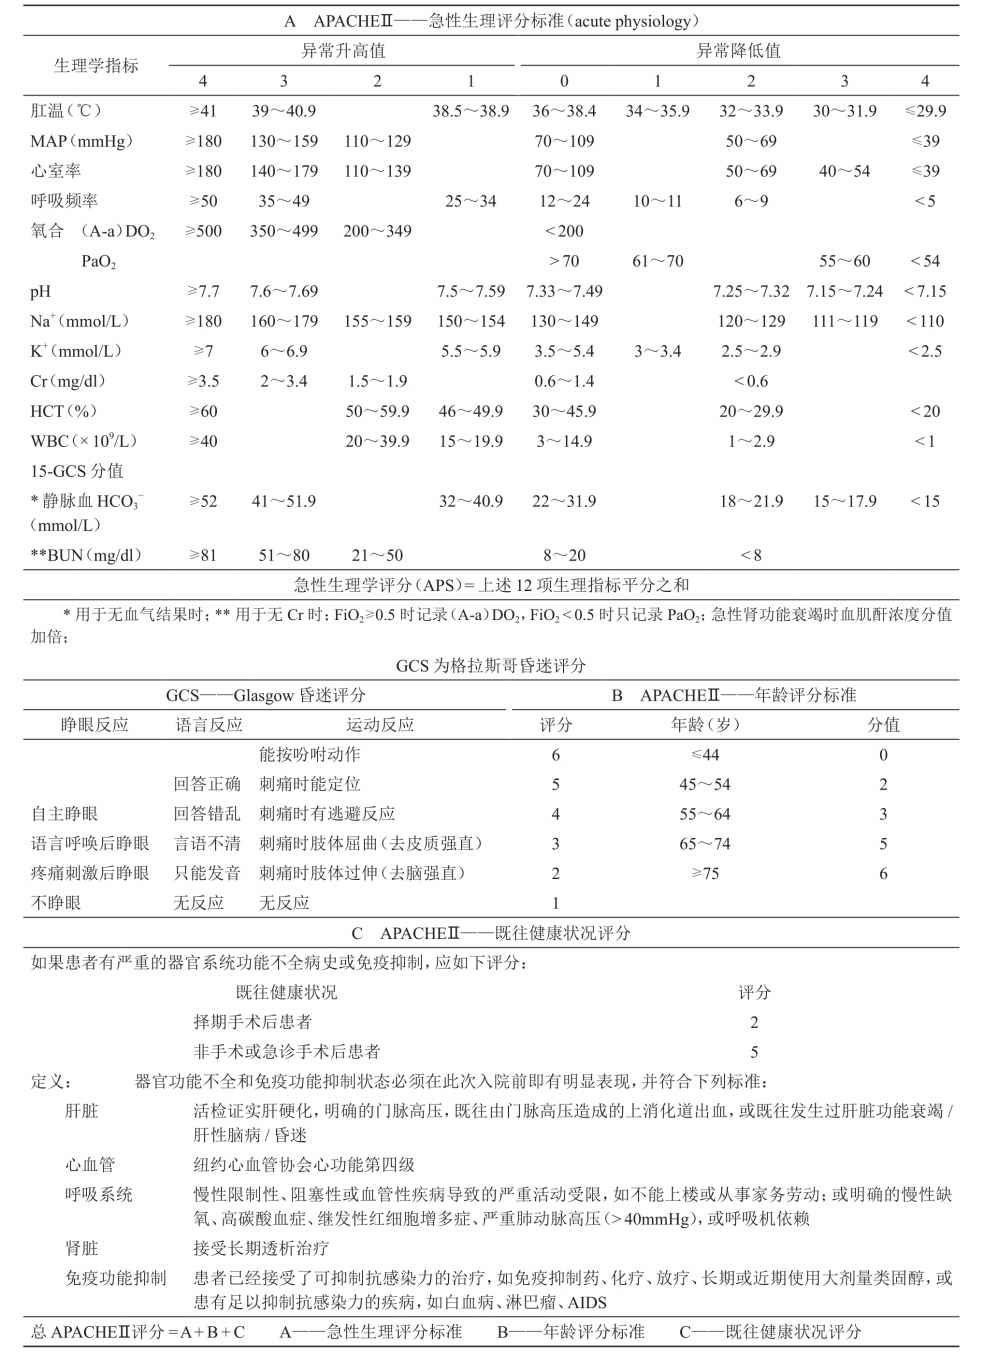
\includegraphics[width=6.78125in,height=9.34375in]{./images/Image00535.jpg}
\end{table}

香港一家医院于1988年5月~1990年10月间,对该院1573例ICU患者(均为华人)以APACHEⅡ评分系统进行了验证,结果:①从APACHEⅡ评分与死亡风险的相关性、预测死亡数与患者实际死亡数有很相似的结果看,认为该系统对原定人群以外的卫生系统(香港)和人种(华人)也是适用的。②该评分系统对个别病例的预测结果缺乏足够的准确性,但也有助于临床的判断。③年龄不足以成为影响转归的预测变量,年龄与死亡间的关系的密切程度在大幅下降(从57.5\%降至29.7\%)。

\hypertarget{text00401.htmlux5cux23CHP16-14-1-1-2}{}
(二) APACHEⅢ评分系统

于1991年由Knaus等在APACHEⅡ基础上又作了较大幅度的修正。他们共收集了美国40家医院内、外科ICU
17
440名患者的临床资料,重点研究分析了五大类预测变量与预后转归的关系(即主要疾病分类、急性生理学异常、年龄、既往功能障碍情况、主要伴随疾病及入ICU前的治疗处所),并用多元判别回归统计方法重新选择变量及设置变量的权数,增加了五个符合统计学上最低限度建模标准的新变量(尿量、血BUN、血白蛋白、血胆红素和血糖),去掉了血清钾、血HCO\textsubscript{3}
\textsuperscript{−}
两个不符合最低限度统计学标准的变量;并简化了Glasgow昏迷评分系统。APACHEⅢ中每项急性生理学指标的测定值均为ICU后24小时之内最不正常时的检测值。

\begin{table}[htbp]
\centering
\caption{APACHEⅢ年龄评分值标准}
\label{tab147-2}
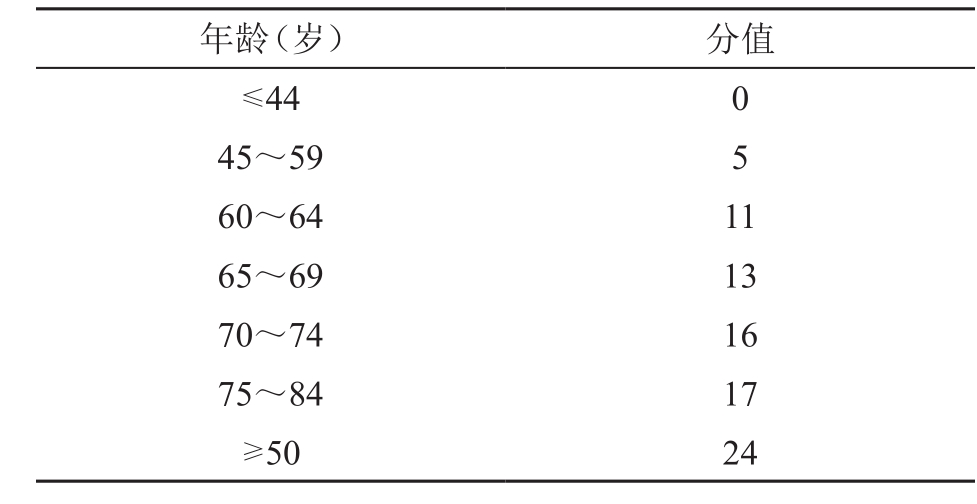
\includegraphics[width=3.25in,height=1.66667in]{./images/Image00536.jpg}
\end{table}

APACHEⅢ预测系统由两部分组成:①APACHEⅢ危重病评分系统,据此可对每例ICU患者的危重程度作出初步估计和分类(表\ref{tab147-2}~表\ref{tab147-5})。②APACHEⅢ预测方程(APACHEⅢ
predictive
equation),把每个ICU患者对APACHEⅢ危重病评分、主要疾病分类系统和入ICU前治疗系统代入此方程,即可得出每个患者死亡风险率。

死亡率预测方程:

ln(R/1 − R)=入ICU主要疾病分数+入ICU前治疗所处评分+ 0.0537 ×
APACHEⅢ评分

R:预测死亡率

APACHEⅢ评分每增加5分,死亡相对危险性增加1.10~1.78。比APACHEⅡ预测准确性高,总预测正确率为88.2\%,而APACHEⅡ为85.5\%。

APACHEⅢ在临床上的应用报道尚少,APACHEⅡ和APACHEⅢ两种评分比较应用,最近国内已有报道。APACHEⅡ和APACHEⅢ的组成基本相同,均包括急性生理学参数、年龄及既往健康状况三部分,两者的区别见表\ref{tab147-6}。

\begin{table}[htbp]
\centering
\caption{APACHEⅢ伴随疾病评分标准}
\label{tab147-3}
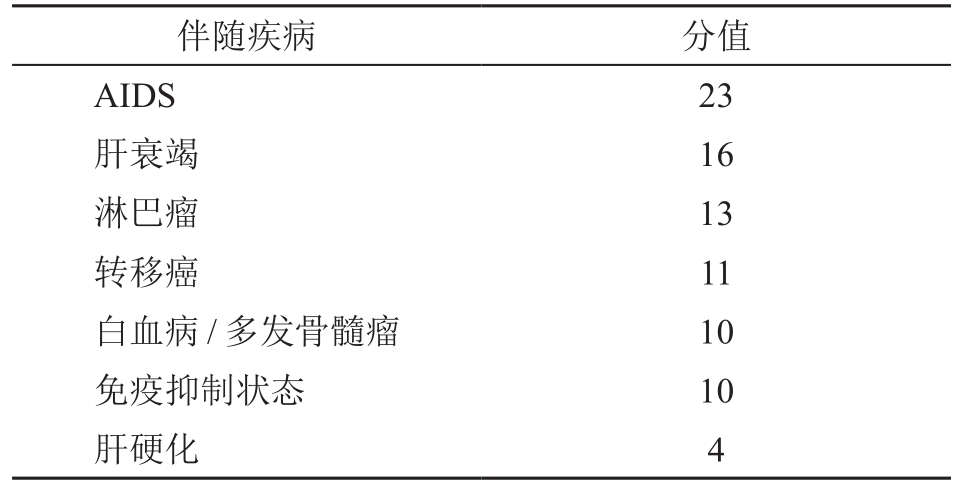
\includegraphics[width=3.25in,height=1.625in]{./images/Image00537.jpg}
\end{table}

\begin{longtable}{c}
 \caption{APACHEⅢ急性生理学异常评分标准(1)~(5)}
 \label{tab147-4}
 \endfirsthead
 \caption[]{APACHEⅢ急性生理学异常评分标准(1)~(5)}
 \endhead
 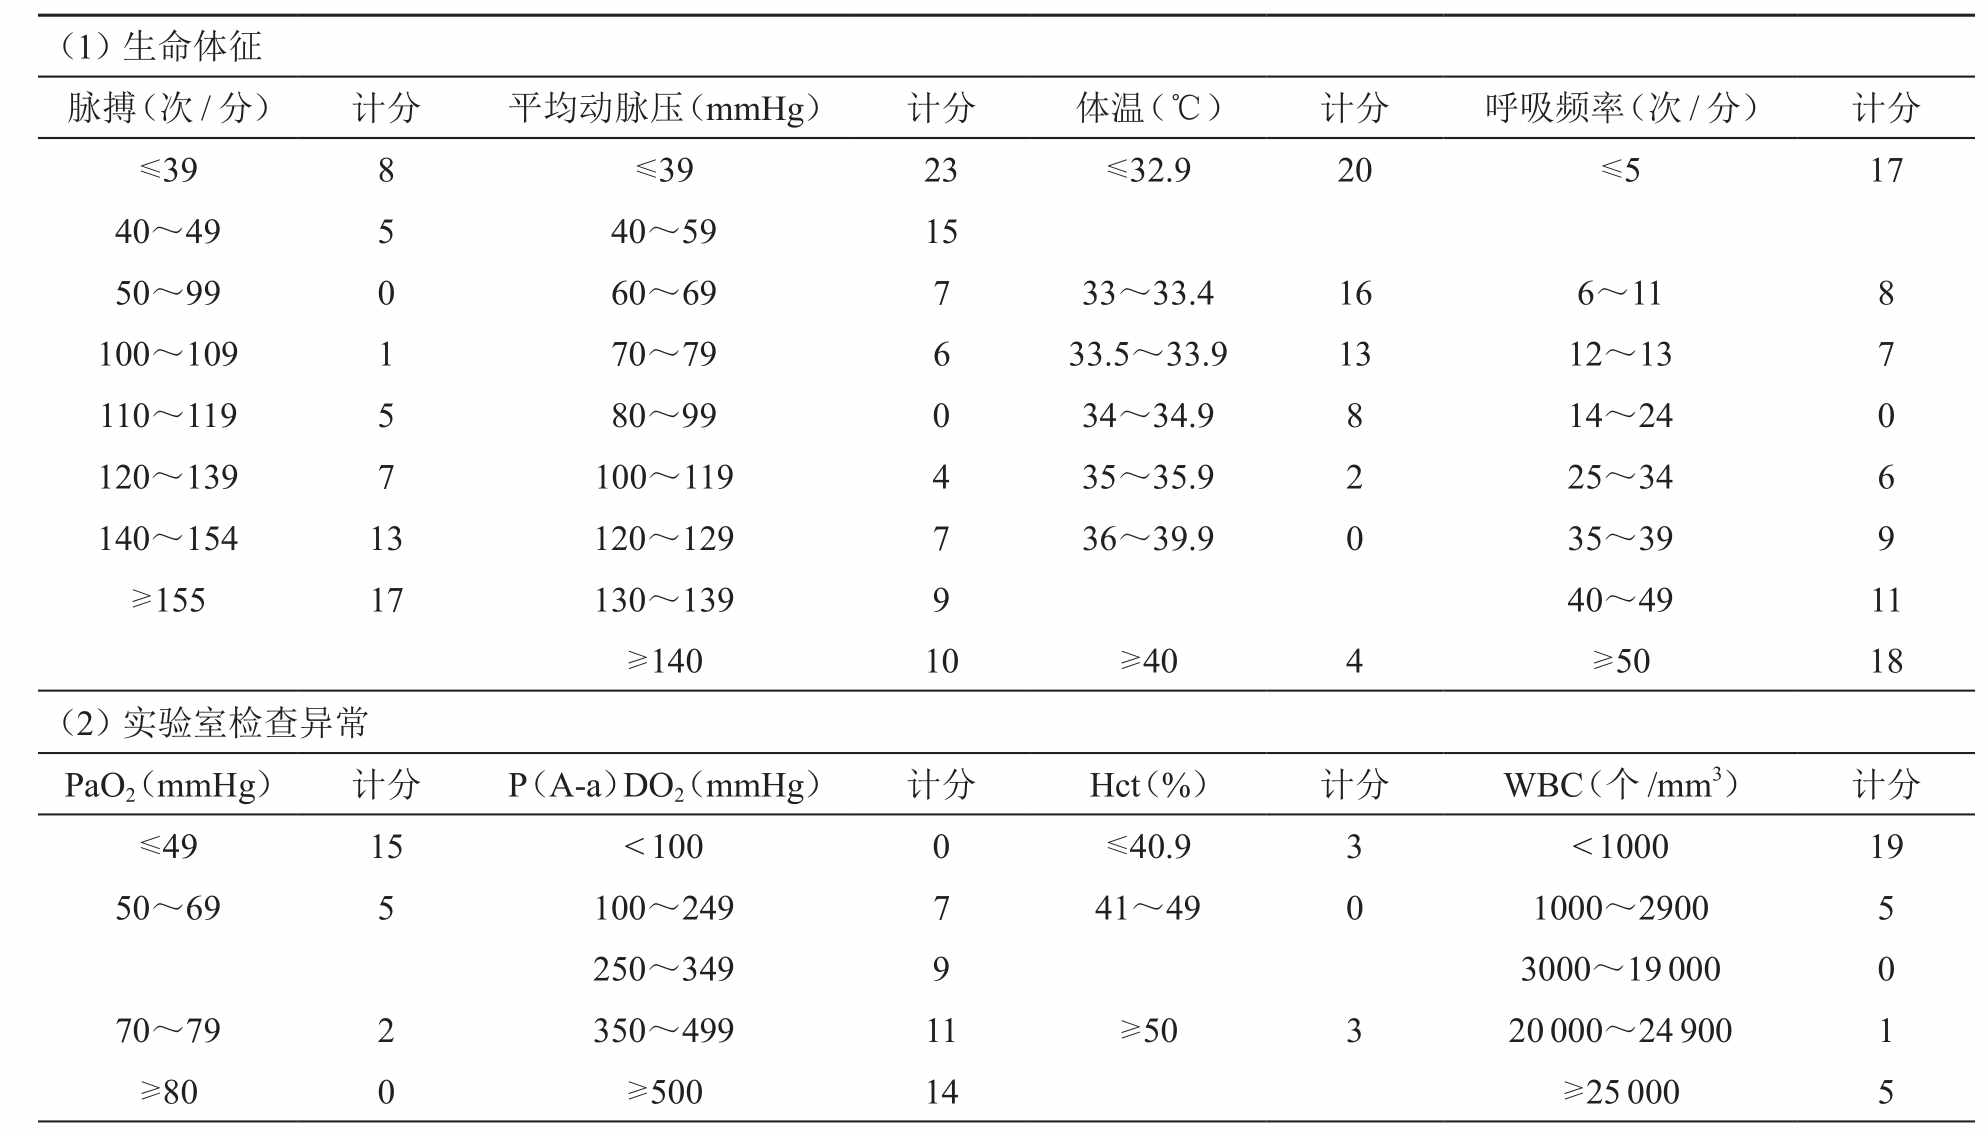
\includegraphics[width=\textwidth,height=\textheight,keepaspectratio]{./images/Image00538.jpg}\\
 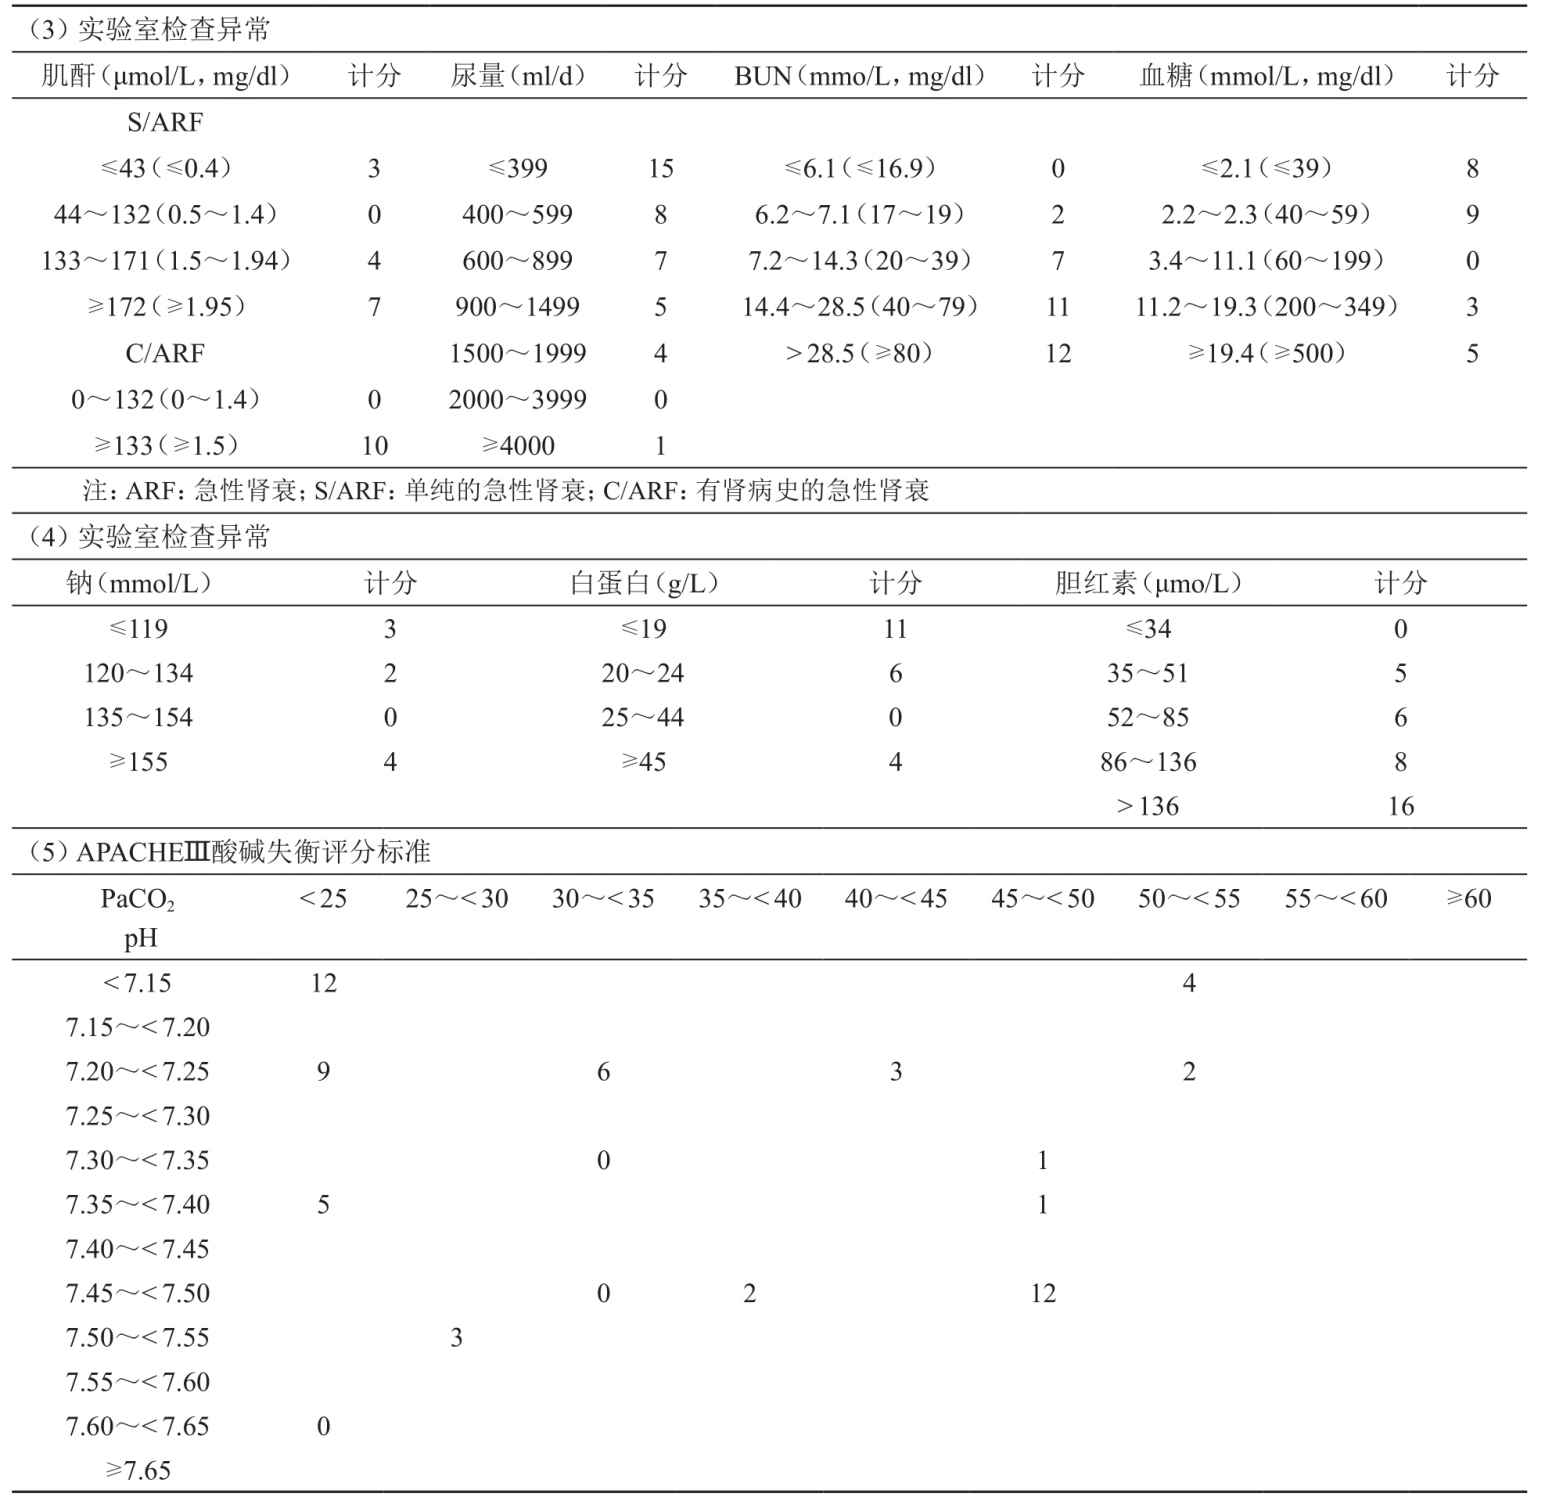
\includegraphics[width=\textwidth,height=\textheight,keepaspectratio]{./images/Image00539.jpg}
 \end{longtable}

\begin{table}[htbp]
\centering
\caption{APACHEⅢ神经系统异常评分标准(1)~(2)}
\label{tab147-5}
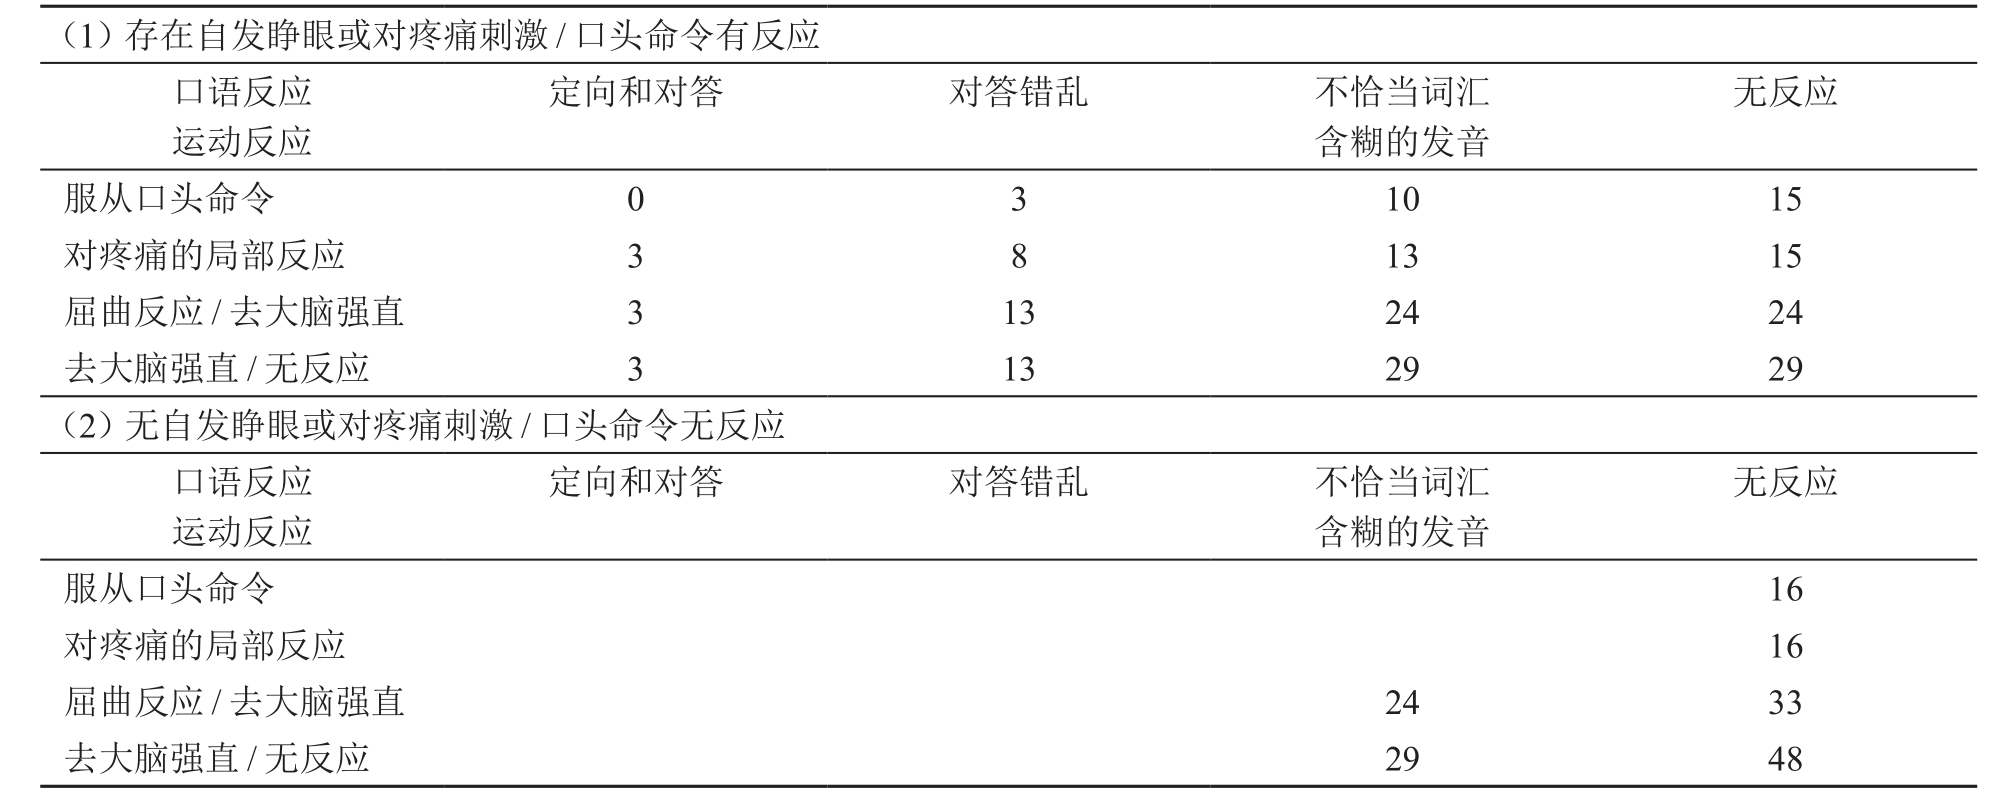
\includegraphics[width=6.6875in,height=2.63542in]{./images/Image00540.jpg}
\end{table}

\begin{table}[htbp]
\centering
\caption{APACHE Ⅱ和APACHE Ⅲ的比较}
\label{tab147-6}
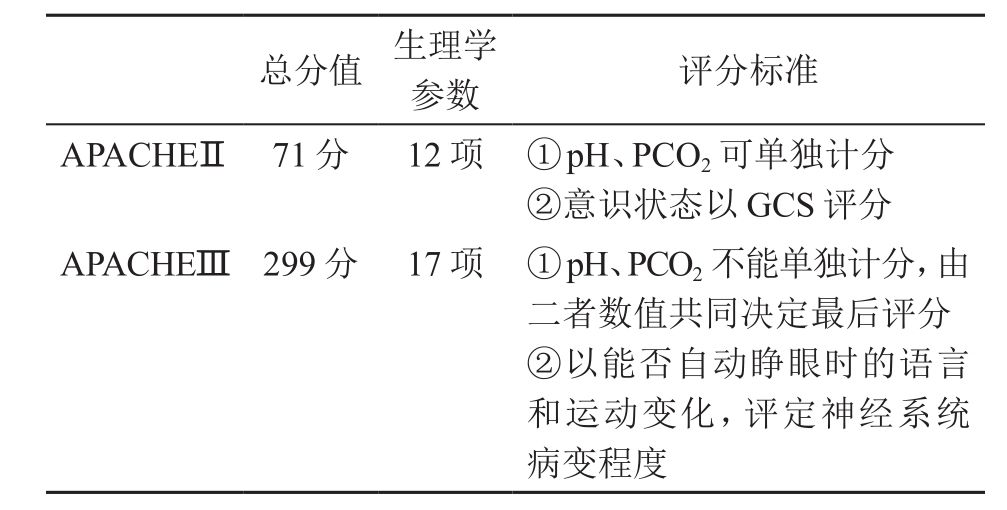
\includegraphics[width=3.34375in,height=1.6875in]{./images/Image00541.jpg}
\end{table}

\subsubsection{简化急性生理学评分系统}

简化急性生理学评分(simplified acute physiology score,SAPS)是由法国Le
Gall等于1984年对于APACHE中的APS部分进行简化而提出的。最后保留了年龄和13项较易获得的13项变量(表\ref{tab147-7}),他们在研究中应用此法在对679例ICU患者病情评估中,显示出评分越高,死亡率越高,≤4分者无死亡,≥21分者死亡率81.4\%
±
5.4\%。其特异性82\%,灵敏度56\%,比较适于规模较小、检测仪器不全、病种单一的ICU患者病情的评估。

后来经过进一步在欧洲、北美等地120家13 152例的多中心研究,Le
Gall等于1993年又提出了SAPSⅡ。与SAPS比较SAPSⅡ减去了原来的呼吸频率、血糖和血细胞比容,增加了PaO\textsubscript{2}
/FiO\textsubscript{2}
(动脉血氧分压与吸入氧浓度之比)和血胆红素;加入了患者既往所患慢性病情况和住院类别,调整了生理学参数的权数(表\ref{tab147-8})。

预测评分系统之间的相互比较:评价各预测评分系统的精确度,可以通过统计学方法进行。如R\textsuperscript{2}
、总分数正确率、发作程度和ROC(receiver operating
characteristic)等参数。或把预测评分系统中的危重病评分演变为预测死亡率更有临床价值的比较方法。

\subsection{死亡概率预测}

死亡概率预测模型(MPM):

MPM评分系统:Lemeshow
S等,1981年首次提出MPM评分系统,经13个国家139家医院的多中心研究,于1993年推出第二版MPM(MPMⅡ)包括MPM\textsubscript{0}
(入院时)和MPM\textsubscript{24}
(入院后24小时内)两个系统。MPM\textsubscript{0}
所选出的指标包括年龄、心率等生理指标、慢性疾病状况、急性病诊断共15项指标。与MPM\textsubscript{0}
相比,MPM\textsubscript{24}
所筛选出的指标并不相同。此系统没有给出各个生理参数的分值,而是用统计分析得出的公式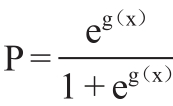
\includegraphics[width=0.57292in,height=0.34375in]{./images/Image00542.jpg}
计算死亡危险性。各项指标满足某个条件则得分为1,否则为0。

g(x)的计算方法为:g(x)= β\textsubscript{0} + β\textsubscript{1}
X\textsubscript{1} +\ldots{}+ β\textsubscript{k} X\textsubscript{k}

β为指标的系数,e为自然对数。与SAPS和APACHE相比,MPMⅡ有两大特点:①包括入院时情况的评分系统,比前两者更适用于在入院后24小时内死亡或离开的患者;②MPM所包括的指标更少也更容易获得。MPM最近经过多次修改以适应评价ICU患者及住入ICU后24小时、48小时和72小时的死亡率,其中MPM、ICU入住模型是唯一的在入住ICU即刻评价住院病死率的系统。24小时、48小时和72小时模型反映患者治疗后的状态以及根据住ICU期间的资料预测住院死亡率。在13个国家的137个ICU临床应用后证实MPMⅡ有很好的实用价值。

\subsection{多器官功能障碍评价}

危重病患者往往存在多器官功能障碍综合征(multiple organ dysfunction
syndrome,MODS)。因此,临床上也常常使用器官功能障碍的数目来简要说明病情的严重程度。研究表明,无论采用何种标准判定器官功能障碍,病死率总是与功能障碍的器官数目呈正相关。关于多器官功能障碍综合征,目前国内外尚无统一的、公认的诊断标准。即使是2008年国际脓毒症指南,定义严重脓毒症时(感染伴有器官血流灌注不足或功能障碍),也只是应用了血乳酸、尿量、外周循环障碍、意识状态这几个指标简要说明。国内首都医科大学附属北京友谊医院王宝恩、张淑文教授牵头的课题组经过前瞻性、多中心临床研究收集、分析了1087
例MODS临床资料建立MODS诊断标准如下。

\begin{table}[htbp]
\centering
\caption{SAPS评分系统}
\label{tab147-7}
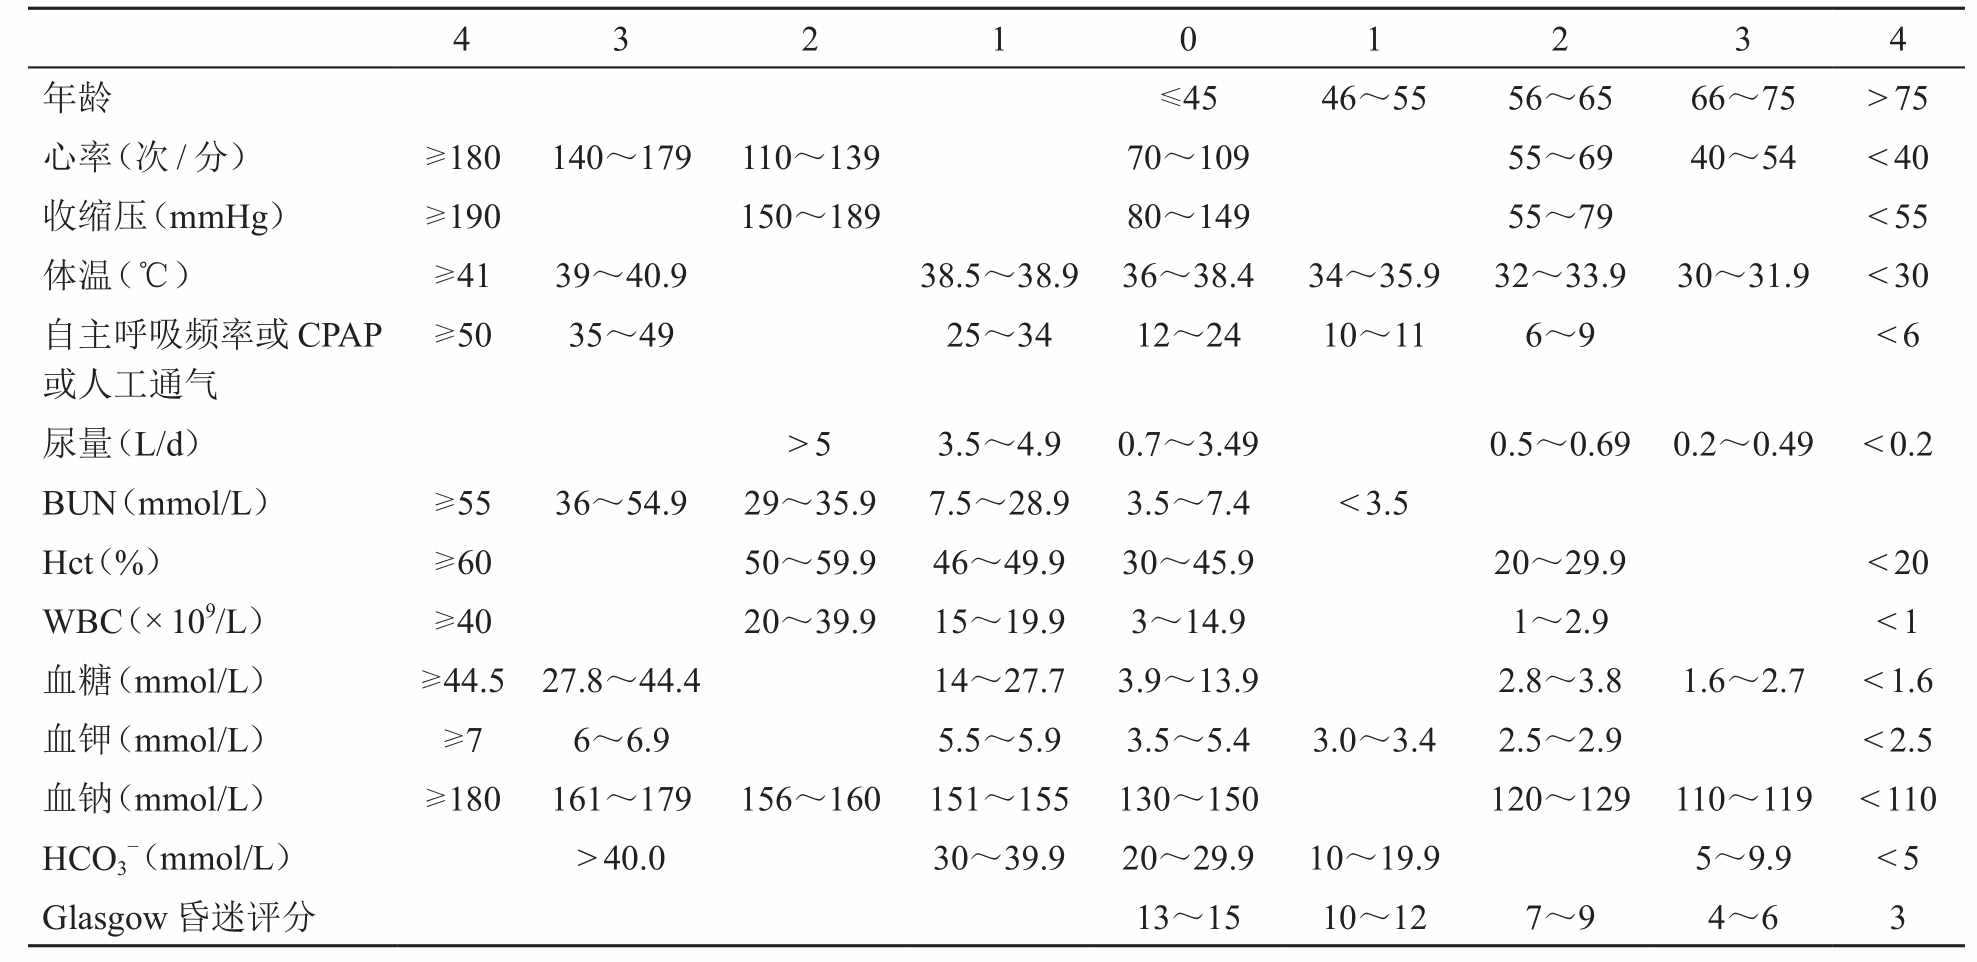
\includegraphics[width=6.58333in,height=3.19792in]{./images/Image00543.jpg}
\end{table}

\begin{table}[htbp]
\centering
\caption{SAPSⅡ评分系统}
\label{tab147-8}
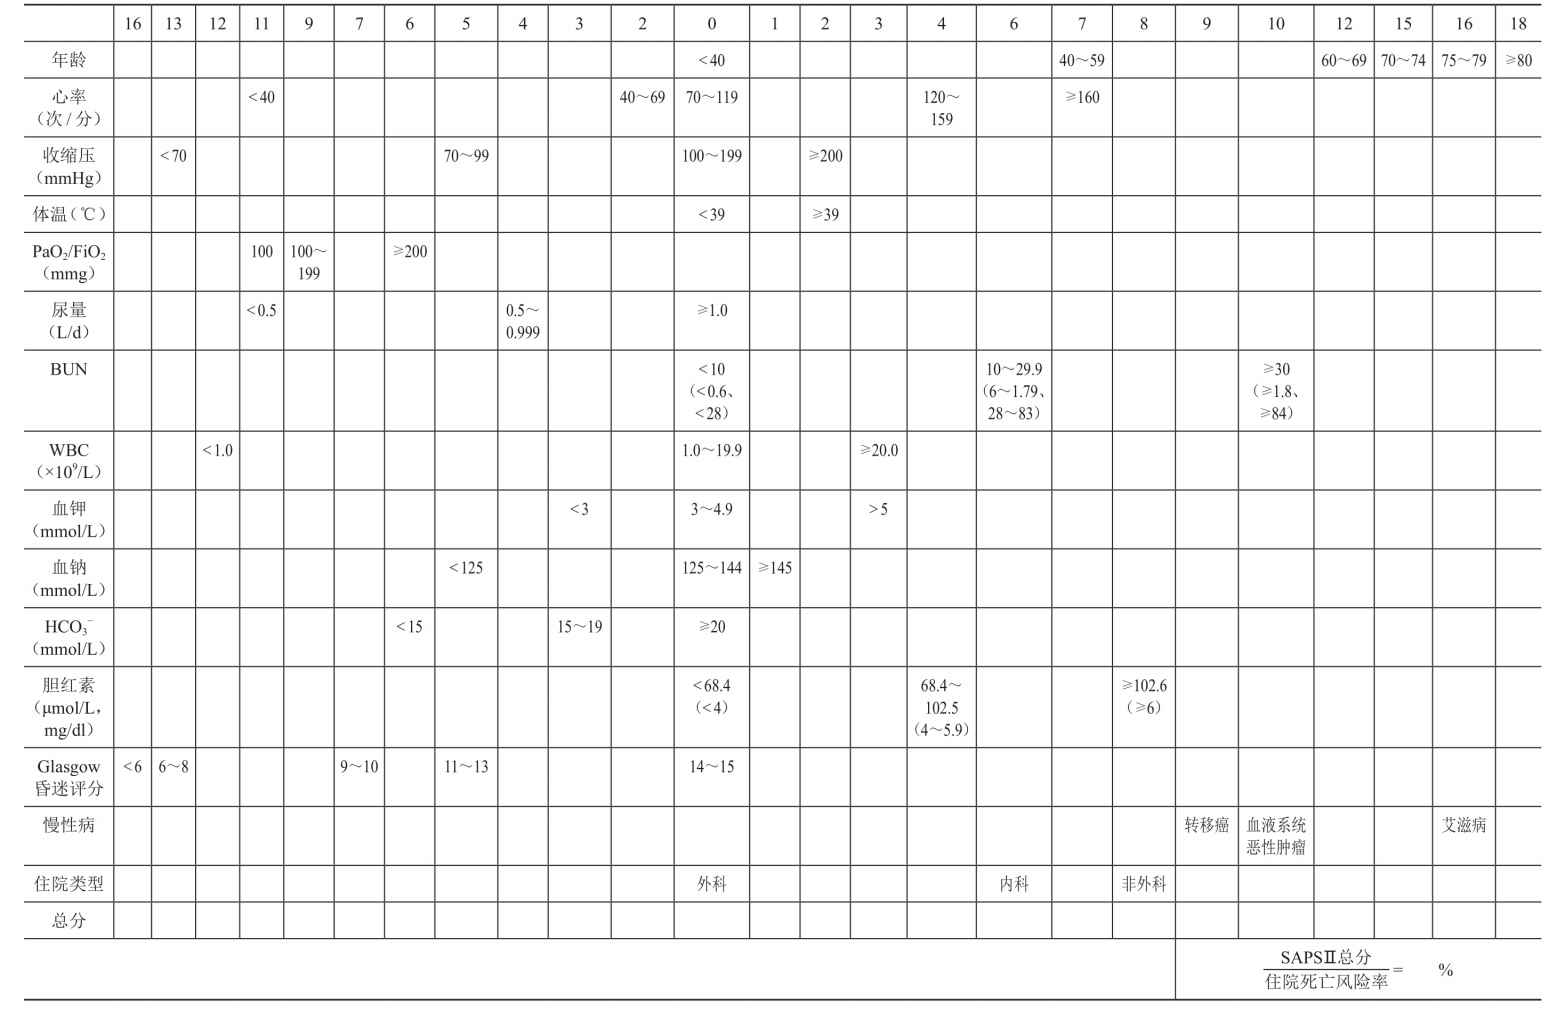
\includegraphics[width=9.72917in,height=6.36458in]{./images/Image00544.jpg}
\end{table}

多器官功能障碍综合征是临床常见的危重症,是指严重感染、创伤、休克、大手术、重症胰腺炎等原发病发生24小时后,机体同时或序贯发生两个或两个以上器官或系统功能障碍的临床综合征。在有上述原发病因的前提下,如果两个或者两个以上器官或系统功能符合下述器官功能障碍的判定标准,则可诊断为多器官功能障碍综合征(MODS)。

本诊断标准纳入心血管、呼吸、中枢神经、凝血、肝脏、肾脏、胃肠共7个脏器系统,用于反映脏器功能障碍的指标和判定标准如下:

1.心血管功能障碍诊断标准 ①收缩压(SBP)SBP
<90mmHg;②平均动脉压(MAP)<
70mmHg;③发生休克、室性心动过速或室颤等严重心律失常、心肌梗死。具备第①,②,③项之一,即可诊断。

2.呼吸系统功能障碍的诊断标准 氧合指数<300mmHg。

3.中枢神经功能障碍诊断标准
①意识出现淡漠或躁动、嗜睡、浅昏迷、深昏迷;②Glasgow昏迷评分≤14分。具备第①,②项之一,即可诊断。

4.凝血系统功能障碍诊断标准 ①血小板计数(PLT)< 100 ×
109/L;②凝血时间(CT)、活化部分凝血酶原时间(APTT)、凝血酶原时间(PT)延长或缩短;3P试验阳性。具备第①,②项之一,即可诊断。

5.肝脏系统功能障碍(借鉴以往的诊断标准)血总胆红素(TBIL)>
1.2mg/dl;血白蛋白(ALB)<
2.8mg/dl。具备第①,②项之一,即可诊断。肾脏系统功能障碍诊断标准
①血肌酐(Cr)> 1.4mg/dl;②尿量<
500ml/24h。具备第①,②项之一,即可诊断。

6.胃肠系统功能障碍
①肠鸣音减弱或消失;②胃引流液、便潜血阳性或出现黑便、呕血;③腹内压(膀胱内压)大于等于11cmH\textsubscript{2}
O。具备第①,②,③项之一,即可诊断。

除了应用器官功能障碍的数目评估病情的严重程度,临床上也采用器官功能障碍量表(即评分系统)评估危重病严重程度。器官功能障碍评分的制订是为了描述危重病的过程而不是为了预测结果,其作为器官功能障碍的测量方法因其有效性而被广泛接受。进入ICU当天计算器官功能障碍评分可评估治疗前器官功能障碍的严重程度。这种评估有几个作用。首先,了解疾病严重程度。它使临床医生了解患者需要ICU进行脏器功能支持的程度,有助于人员、物质的分配,脏器功能支持成功的可能性。其次,通过对器官功能障碍的评估来讨论治疗的需要及其局限性。另外,计算基础器官功能障碍评分有助于临床ICU研究的医生选择合适的研究人群(如排除情况过好和过差不能从治疗中获益的患者)。

常见的MODS评分系统有以下4种。国内危重病医学专家在1995年讨论制订了“多脏衰病期分期诊断及严重程度分期标准(1995)”(表\ref{tab147-9}),加拿大学者Marshall在1995年制订了MODS评分系统(表\ref{tab147-10}),欧洲危重病学会在1996年制订SOFA评分(表\ref{tab147-11}),国内首都医科大学附属北京友谊医院王宝恩、张淑文教授牵头的课题组经过前瞻性、多中心临床研究收集、分析了1087例MODS临床资料总结出的MODS评分系统(表\ref{tab147-12})。这些器官功能障碍评分在评价危重病病情严重程度方面都有一定的价值。

\begin{longtable}{c}
 \caption{多脏衰病期分期诊断及严重程度分期标准(1995)}
 \label{tab147-9}
 \endfirsthead
 \caption[]{多脏衰病期分期诊断及严重程度分期标准(1995)}
 \endhead
 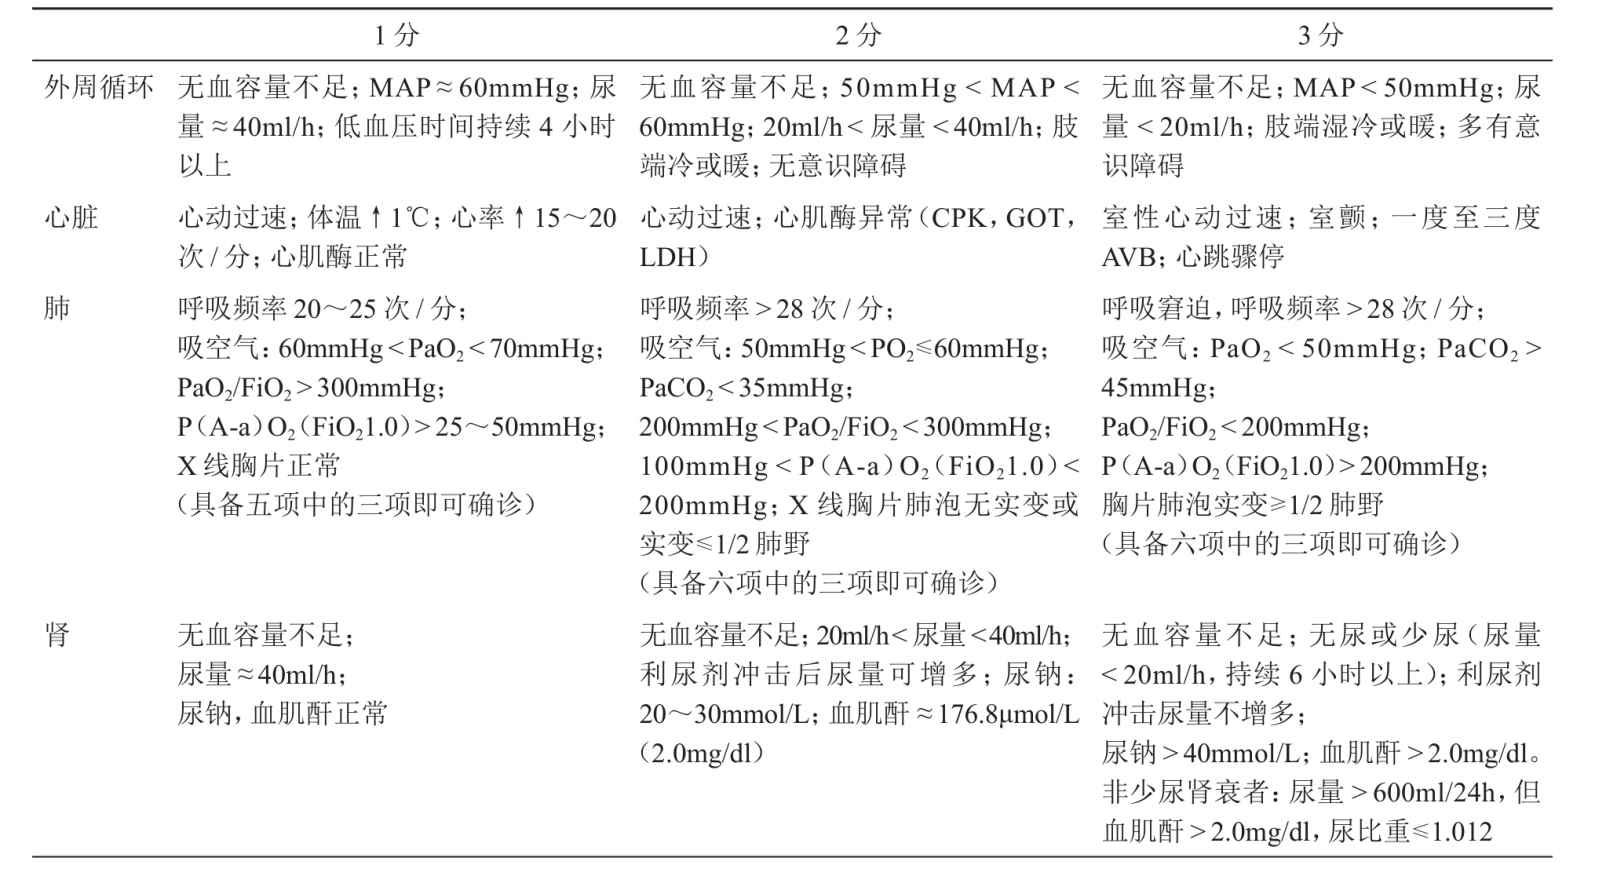
\includegraphics[width=\textwidth,height=\textheight,keepaspectratio]{./images/Image00545.jpg}\\
 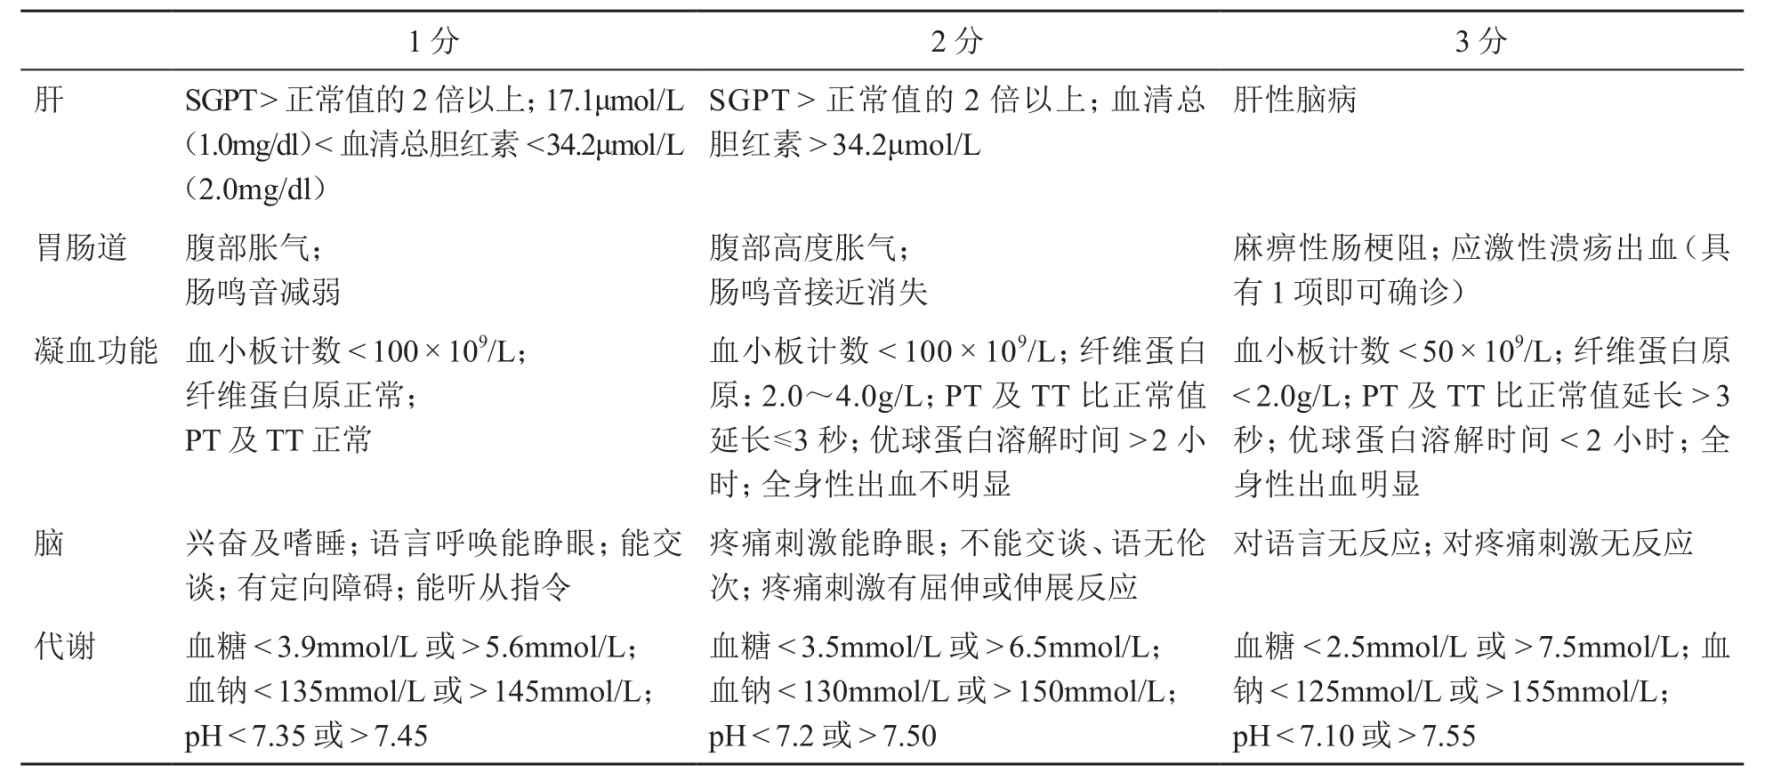
\includegraphics[width=\textwidth,height=\textheight,keepaspectratio]{./images/Image00546.jpg}
 \end{longtable}

注:1分:器官功能轻度障碍,2分:中度障碍,3分:衰竭

\begin{table}[htbp]
\centering
\caption{Marshall MODS评分标准}
\label{tab147-10}
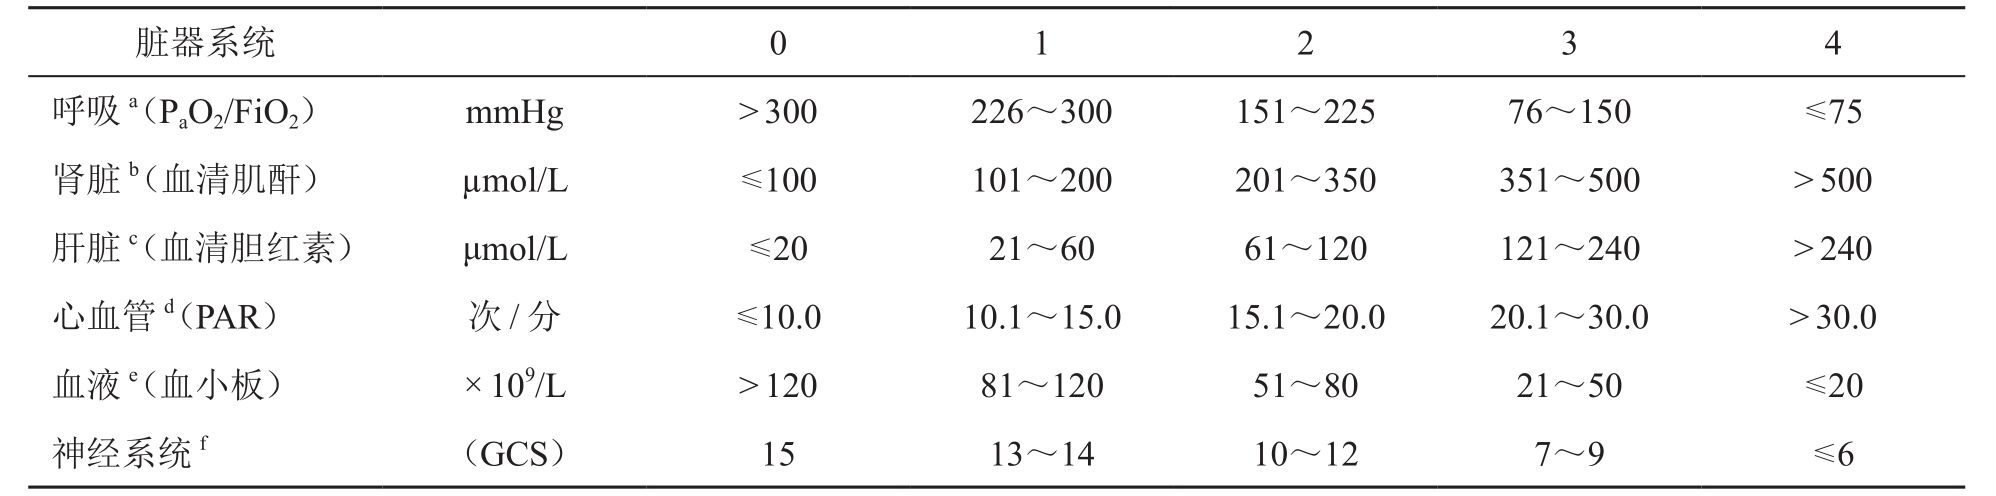
\includegraphics[width=6.64583in,height=1.64583in]{./images/Image00547.jpg}
\end{table}

注:a:计算PaO\textsubscript{2} /FiO\textsubscript{2}
时不考虑是否使用机械通气及机械通气的方式,也不考虑是否应用呼吸末正压(PEEP)及PEEP值的大小;b:计算血清肌酐时,单位是µmol/L,不考虑是否接受透析治疗;c:血清胆红素的单位是μmol/L;压力调整后心率(the
pressure-adjusted heart
rate,PAR))=心率×(中心静脉压/平均动脉压);e.血小板的单位是×
10\textsuperscript{9}
/L;f:GCS最好由患者的护士计算,保守计分(对于接受镇静剂或肌松剂的患者,可假定其神经功能正常,除非有意识障碍的证据);1kPa
= 7.5mmHg

\begin{table}[htbp]
\centering
\caption{SOFA评分系统(1996年)}
\label{tab147-11}
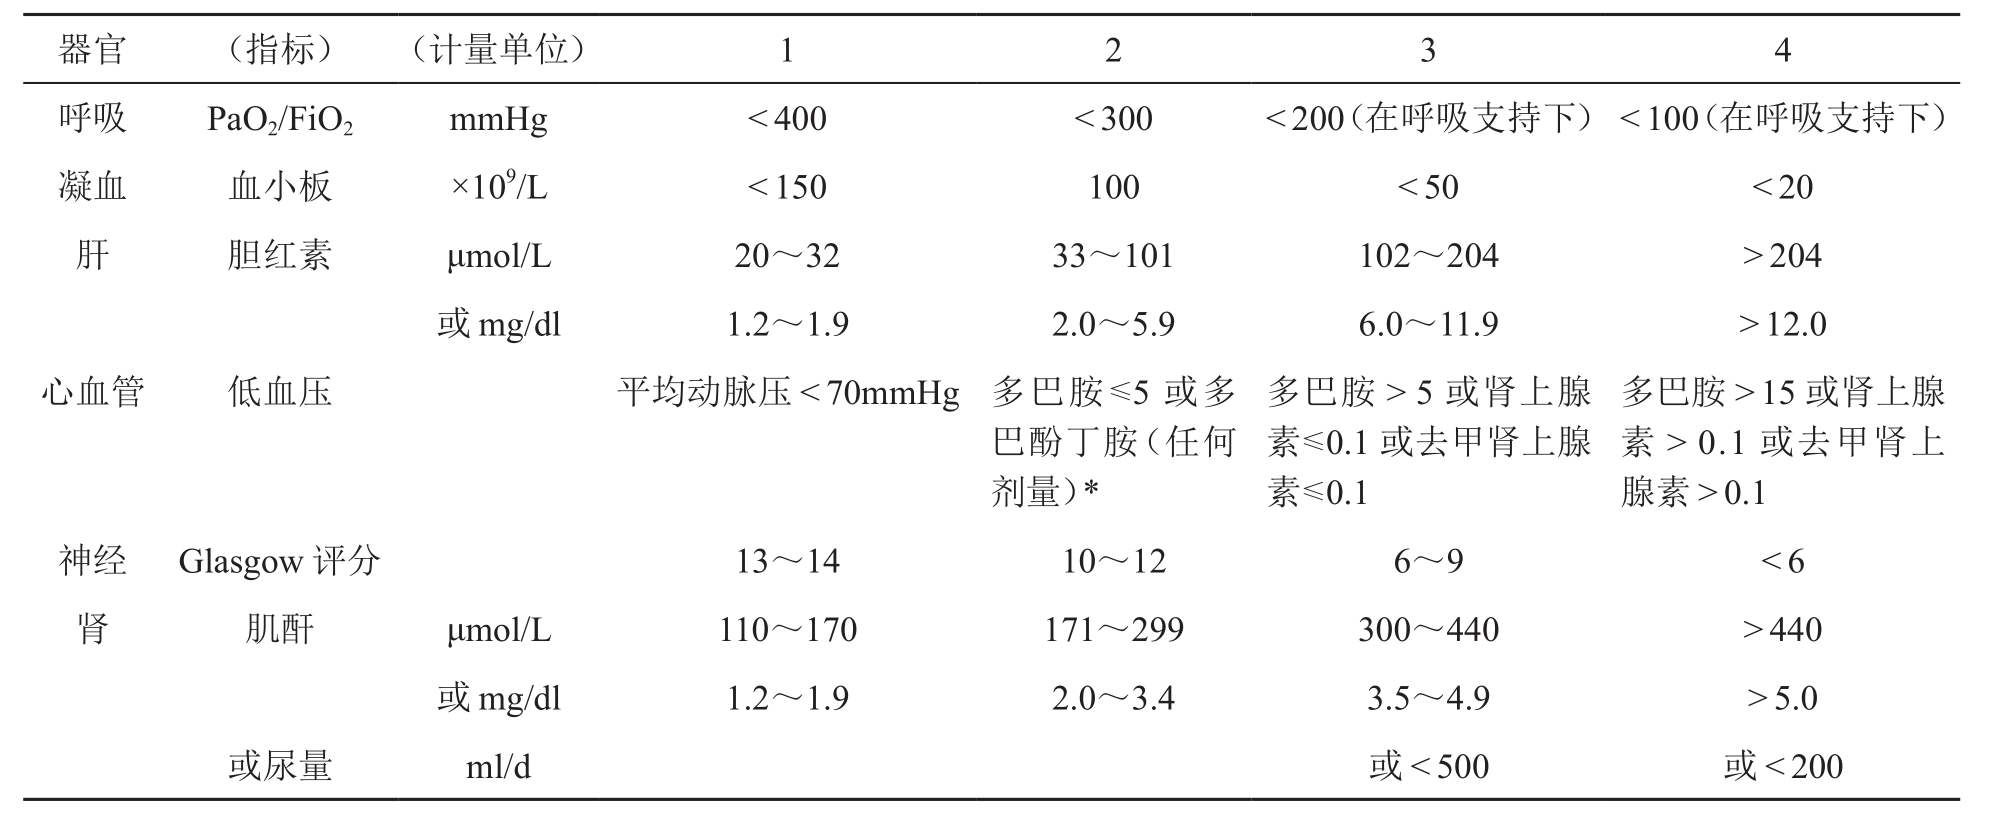
\includegraphics[width=6.66667in,height=2.70833in]{./images/Image00548.jpg}
\end{table}

*注:肾上腺素能药物至少输注1小时(剂量为μg/kg•min)

\begin{table}[htbp]
\centering
\caption{MODS评分系统(2007年)}
\label{tab147-12}
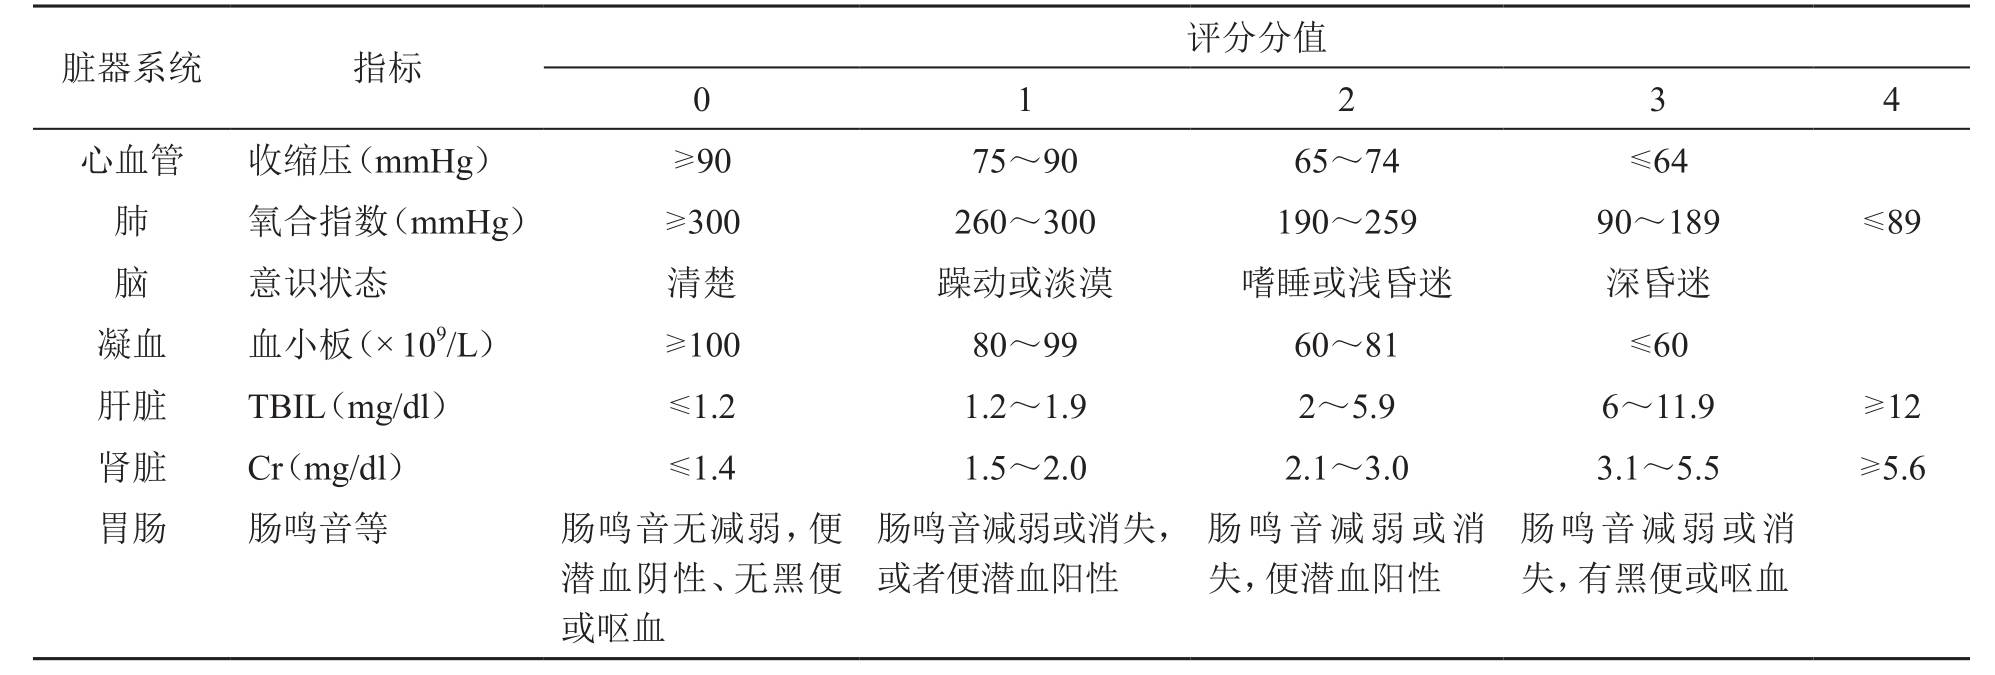
\includegraphics[width=6.64583in,height=2.23958in]{./images/Image00549.jpg}
\end{table}

\subsection{危重病严重程度评估方法的临床应用}

1.应用于急诊临床、特别是急救医学领域的科学研究

预测评分系统可帮助研究人员对患者按照严重程度的预测死亡率进行分层,再随机分组,保证了死亡率和分组的随机性。近年,还有人提出对死亡率的预测和多变量统计学方法处理,可减少临床研究中实验组和对照组达到统计学差异所需的观察例数。

2.应用于 ICU医疗质量的评估
预测评分系统的制订,为急诊临床对危重病患者病情严重程度的判断提供了一个比较客观的、定量化的统一标准;特别是预测评分系统所计算出的预测死亡率与ICU实际死亡率差值的比较,被认为是评价不同ICU医疗质量的一个较为直观的指标,差值越大,说明医疗质量越高,因此是很值得推广应用的。

3.帮助确定 ICU患者治疗方案
通过上面介绍,APACHE预测评分系统及SAPS评分系统均有较大的临床应用价值,又各具特点,对临床治疗方案的制订,无疑会有很大帮助,现业已在国内外逐渐应用起来。

4.评分系统为科学评估危重患者的病情提供了依据

根据评分高低可以判断病情
,一般认为评分越高,病情越重;能较可靠地预测群体患者的死亡率,无论MPM还是APACHE均可对患者死亡危险性进行计算,从而预测是否有望获救;为医生、家属、社会作出医疗决策提供客观依据。危重患者抢救往往耗时、耗力、耗资巨大,有时会出现高代价低回报的情况,造成医疗资源浪费,家庭和社会的负担加重,甚至造成医疗纠纷,有了评分系统可以客观分析,从而做出合理的医疗决策;可对监护患者所需要的监测选择性操作进行预测和评估,从而指导第二个24小时操作,或对低风险监护收容患者进行宏观控制,以充分发挥ICU的效益,指导资源的合理投向;在临床追踪、非随机性或多中心临床研究中非常有用,可以控制观察对象的均一性;可帮助确定医院ICU所需床位数,医生、护士、患者之比,评价ICU工作效益以及对医疗费用进行评估,为医疗改革提供依据。

上述各预测评分系统是否完全适合我国具体情况,还有待于临床应用验证。近年国内学者也在探索,以求制订出适合我国应用的危重病评分方法。

\protect\hypertarget{text00402.html}{}{}

\hypertarget{text00402.htmlux5cux23CHP16-14-5}{}
参 考 文 献

1. Knaus WA,Draper EA,Wagner DP,et al. APACHE II:a severity of
disease classification system. Crit Care Med,1985,13(10):818-829

2. Knaus WA,Wagner DP,Draper EA,et al. The APACHE Ⅲprognostic system.
Risk prediction of hospital mortality for critically ill hospitalized
adults. Chest,1991,100(6):1619-1636

3. Le Gall JR,Lemeshow S,Saulnier F. A new Simplified Acute Physiology
Score(SAPS II)based on a European/North American multicenter study.
JAMA,1993,270(24):2957-2963

4. Lemeshow S,Teres D,Klar J,et al. Mortality Probability Models(MPM
II)based on an international cohort of intensive care unit patients.
JAMA,1993,270(20):2478-2486

5. Castella X,Artigas A,Bion J,Kari A. A comparison of severity of
illness scoring systems for intensive care unit patients:results of a
multicenter,multinational study. The European/North American Severity
Study Group. Crit Care Med,1995,23(8):1327-1335

6. Marshall JC,Cook DJ,Chrisstou NV,et al. Multiple organ dysfunction
score reliable descriptor of a complex clinical outcome. Crit Care
Med,1995,23(10):1638-1652

7. JL Vincent,R Moreno,J Takala,et,al. The SOFA(Sepsisrelated Organ
Failure Assessment)score to describe organ dysfunction/failure.
Intensive Care Med,1996,22:707-710

8. R. Phillip Dellinger,Mitchell M. Levy,Jean M. Carlet,et,al.
Surviving Sepsis Campaign:International guidelines for management of
severe sepsis and septic shock:2008. Intensive Care
Med,2008,34(1):17-60

9. 王超
,苏强,张淑文,等.多器官功能障碍综合征诊断标准的前瞻性多中心临床研究.中华外科杂志,2009,47(1):40-43

10. 王超
,苏强,张淑文,等.多器官功能障碍综合征病情严重度评分系统.中国医学科学院学报,2007,29(4):497-500

\protect\hypertarget{text00403.html}{}{}

